% 高一64_格致中学_10月月考.tex
%   —— 高一上数学“2026-2027 年格致中学高一上 10 月月考”（讲评版）
% 试卷版：xelatex 高一64_格致中学_10月月考.tex
% 答案版：xelatex "\def\isanswer{1}% 高一64_格致中学_10月月考.tex
%   —— 高一上数学“2026-2027 年格致中学高一上 10 月月考”（讲评版）
% 试卷版：xelatex 高一64_格致中学_10月月考.tex
% 答案版：xelatex "\def\isanswer{1}% 高一64_格致中学_10月月考.tex
%   —— 高一上数学“2026-2027 年格致中学高一上 10 月月考”（讲评版）
% 试卷版：xelatex 高一64_格致中学_10月月考.tex
% 答案版：xelatex "\def\isanswer{1}% 高一64_格致中学_10月月考.tex
%   —— 高一上数学“2026-2027 年格致中学高一上 10 月月考”（讲评版）
% 试卷版：xelatex 高一64_格致中学_10月月考.tex
% 答案版：xelatex "\def\isanswer{1}\input{高一64_格致中学_10月月考.tex}"
% 紧凑版：xelatex "\def\iscompact{1}\input{高一64_格致中学_10月月考.tex}"
%
% 原始材料：微信公众号“魔都数学加油站”文章，作者破晓，连载“27学年高一64”；
% 原文标题“27学年高一64——2026-2027年上海市格致中学高一上10月月考”；
% 原文链接：https://mp.weixin.qq.com/s/0DfB77nTJf7NdVI_FYXxeA。
% 页面标注发布时间 2026-10-17 21:58（上海）。
% 本次转录只据 `原图/高一64_格致中学_10月月考/` 的 14 张 PNG 逐页读图。
% 正文为 14 张 PNG 页（`01..14.png`）：第 12、13、14 页 2560×3620，
% 第 01—11 页 4762×6735（**同一篇各页分辨率不同**），均按页序读取。
% 14 页全为试卷正文页（卷首标题在第 1 页页顶，卷末解答题第 18 题解析止于第 14 页），
% 无封面页、目录页、二维码或宣传页。粉色斜排“魔都数学加油站”为卷面水印，与公众号页脚一并未录入。
%
% 卷首标题：照卷面印作“2026--2027 年格致中学高一上 10 月月考”，年份区间按全稿惯例排 en dash。
% 原卷只有一行标题、无副标题。
%
% 篇幅与题号：原卷自第 3 题起编号（第 1、2 题不在本卷内）。填空题 3—10（8 题）、
% 选择题 11—14（4 题）、解答题 15—18（4 题），共 16 题。本稿沿用原节与原题号，
% 只改排为全稿统一的大节样式（原卷小节标题为“一、填空题”“二、选择题”“三、解答题”）。
%
% 讲评版：原卷每题下直接印【答案】或【解析】。**只印【答案】的 1 题**（第 5 题），
% 本稿只给 \ans{}；其余 15 题都印【解析】（按全稿口径这类题不另提 \ans{}——第 11、13、14 题
% 的结论写在解析末句（“故选 A”“故选 D”等），亦照录在解析内）。**另有 1 题答案印在题干括号内**——
% 第 12 题（“( B )”，该题无【答案】/【解析】段），本稿按 高一37 第 13 题成例把括号留空、
% 答案另提为 \ans{$B$}。
%
% 副标题：原卷未印副标题。本稿按“知识模块”口径标作“集合与常用逻辑用语、不等式”：
% 16 题中集合与常用逻辑用语 8 题（第 4、9、10、11、12、13、16、18 题），
% 不等式 8 题（含一元二次方程与韦达定理、基本不等式、二次不等式、恒成立、分式不等式：
% 第 3、5、6、7、8、14、15、17 题），两类均达三分之一，故并标。口径同 高一59、高一63。
%
% 与原卷的排版差异：
%   ① 原卷每题下直接印【答案】/【解析】，本稿按全稿惯例将答案与解析置于答案版，试卷版保持干净；
%   ② 原卷未印副标题，本稿按“知识模块”口径补出；
%   ③ 原卷填空横线约三四个字宽，本稿按全稿惯例统一排 \blankline[4.4em]；
%   ④ 原卷实数集排斜体 $R$（第 4、7、8、13、15、18 题）或粗体 $\mathbf{R}$（第 18 题题干与
%      解析共 6 处），整数集排斜体 $Z$（第 9、13 题）或粗体 $\mathbf{Z}$（第 9 题解析末两行），
%      有理数集排粗体 $\mathbf{Q}$（第 13 题选项 A），本稿按全稿惯例统一改用 $\R$、$\Z$、$\Q$
%      （记号归一，粗体／斜体不作区分）；空集记号原卷作 $\varnothing$，照录；
%   ⑤ 第 4 题的补集**原卷用上划线记号 $\bar B$**（题干 1 处、解析 4 处，共 5 处），
%      与全稿惯例的 $\complement_U B$ 不同，本稿照录原卷的 $\bar B$；
%   ⑥ 原卷用描述法时竖线排细竖“$|$”（如 $\{x\mid|x|\geqslant2024\}$ 一类），本稿按全稿惯例排 \mid；
%   ⑦ 第 15—18 题的子问原卷各自另起一行、以“（1）”“（2）”“（3）”标号，本稿按全稿惯例用
%      enumerate 的 (1)(2)(3)；解析中的子问标号一律用 \stepm{(1)}{…}；
%      第 18 题解析中分情形的①②③与分小目的 (i)(ii)，按全稿惯例作 \stepm{①}{…}、\stepm{(i)}{…}；
%   ⑧ 第 13 题解析的“A 选项：”“B 选项：”“C 选项：”“D 选项：”原卷排**加粗**（共 4 处），
%      同 高一63“法一：”成例，本稿排 \stepm{A 选项：}{…} 一类（加粗着色、不改黑色基调），
%      冒号照原卷排全角；
%   ⑨ 第 17 题解析带评分档，原卷在档与档之间排一串点线（“………2 分”），
%      本稿照录为“\dots\dots2 分”一类（同 高一54 成例），共 5 处；
%   ⑩ 选择题的作答括号原卷排半角“(　　)”（第 11、13、14 题括号内空白、第 12 题括号内印 B），
%      本稿按全稿惯例排 \mbox{（\quad）}；选项字母后的句点照原卷排“A.”“B.”；
%   ⑪ 每道解答题原卷未留作答空白，本稿按全稿惯例加 \ansspace（末题用 \ansspace*）；
%   ⑫ 第 17 题题干右侧的十字形八边形示意图，本稿按原卷截图裁出（`figures/cross_octagon_h64.png`，
%      原分辨率裁切，未放大、未用 TikZ 重绘），图内阴影与点名照原卷。
%
% 原卷笔误/存疑（均照录未改，正文对应处另有 % 注）：
%   ① 第 8 题解析末两步自相矛盾：上一步已化为 $\dfrac x{x-1}<0$，下一步却印作
%      “即 $x(x+1)<0$，解得 $-1<x<0$”并给出解集 $(-1,0)$——由 $\dfrac x{x-1}<0$ 应得
%      $x(x-1)<0$、解集 $(0,1)$；已 8 倍放大确认原卷确为 $x+1$ 与 $(-1,0)$，照录未改。
%   ② 第 13 题 D 选项解析“乘法满足结合率”的“率”应为“律”（同段 A、B 选项均作“结合律”）。
%   ③ 第 13 题条件①“任意 $a,b\in G$. 有 $a*b\in G$；”在 $G$ 后印句号（其余三条均以逗号
%      接下文），疑为逗号之误，照录。
%   ④ 第 17 题 (3) 解析把定义域印作 $0<x<2\sqrt{10}$，与 (1) 所得 $0<x<10\sqrt2$ 不一致
%      （疑为 $10\sqrt2$ 之误）；照录未改。
%   ⑤ 第 17 题 (3) 末句“所以 $AD$ 长 $x$ 的取值范围$[\sqrt5,2\sqrt5]$.”脱一个“为”。
%   ⑥ 第 18 题 (3) ③“则 $\dfrac12$ 是方程 $x^2+bx+c=0$ 的**两**实数根”——只有一个数却称
%      “两实数根”，语病；照录。
%
% 插图：第 17 题题干有 1 幅十字形八边形示意图（原卷第 09 页右侧），已按原卷截图排入；
% 其余 13 页无任何图形、无“如图”字样（第 17 题的“图中”均指此图）。
%
\documentclass[a4paper,11pt]{article}
\usepackage{common}

\begin{document}

\examtitlest[3]{2026--2027 年格致中学高一上 10 月月考}{集合与常用逻辑用语、不等式}

\bigsec{一、填空题}

\begin{enumerate}
\setcounter{enumi}{2}

\item 已知一元二次方程 $x^2-nx+5=0$ 的两个实根分别为 $x_1$、$x_2$，且 $\dfrac1{x_1}+\dfrac1{x_2}=1$，则实数 $n$ 的值为\blankline[4.4em].

\ifanswer
\solbegin
\step{$\dfrac1{x_1}+\dfrac1{x_2}=\dfrac{x_1+x_2}{x_1x_2}=\dfrac n5=1$，所以 $n=5$.}
\solend
\fi

\item 全集为 $U=\R$，$A=\{x\mid|x|\geqslant2\}$，$B=\{y\mid y=x^2+1,x\in\R\}$，则 $A\cup\bar B=$\blankline[4.4em].

\ifanswer
\solbegin
\step{由题意得集合 $A=\{x\mid x\geqslant2\text{ 或 }x\leqslant-2\}$，}
\step{因为 $x^2+1\geqslant1$，所以集合 $B=\{x\mid x\geqslant1\}$，所以 $\bar B=\{x\mid x<1\}$，}
\step{则 $A\cup\bar B=\{x\mid x\geqslant2\text{ 或 }x<1\}$.}
\solend
\fi

\item 若 $x>2$，则 $4x+\dfrac1{x-2}$ 的最小值为\blankline[4.4em].

\ifanswer
\ans{$12$}
\fi

\item 已知关于 $x$ 不等式组$\begin{cases}(3x-2)(2x+3)\leqslant0\\ x-a<0\end{cases}$\!没有实数解，则实数 $a$ 的取值范围为\blankline[4.4em].

\ifanswer
\solbegin
\step{由题意得 $\begin{cases}-\dfrac32\leqslant x\leqslant\dfrac23\\ x<a\end{cases}$ 无解，所以 $a\leqslant-\dfrac32$.}
\solend
\fi

\item 若不等式 $\dfrac{x^2-8x+20}{mx^2-mx-1}<0$ 对一切 $x\in\R$ 都成立，则实数 $m$ 的取值范围为\blankline[4.4em].

\ifanswer
\solbegin
\step{因为 $x^2-8x+20=(x-4)^2+4\geqslant4>0$，所以 $mx^2-mx-1<0$，}
\step{当 $m=0$ 时，$mx^2-mx-1=-1<0$，不等式成立；}
\step{设 $y=mx^2-mx-1$，当 $m\neq0$ 时函数 $y$ 为二次函数，$y$ 要恒小于 0，}
\step{抛物线开口向下且与 $x$ 轴没有交点，即 $m<0$ 且 $\Delta<0$，得 $-4<m\leqslant0$，}
\step{故实数 $m$ 的取值范围为 $(-4,0]$.}
\solend
\fi

\item 已知关于 $x$ 的不等式 $\dfrac{ax-1}{x+b}>0$ 的解集为 $\{x\mid-1<x<2\}$，其中 $a$、$b\in\R$，则关于 $x$ 的不等式 $\dfrac{bx+1}{ax+1}<1$ 的解集为\blankline[4.4em].

\ifanswer
\solbegin
\step{不等式 $\dfrac{ax-1}{x+b}>0$ 等价于 $(ax-1)(x+b)>0$，即 $ax^2+(ab-1)x-b>0$，}
\step{所以 $-1$ 和 2 为方程 $ax^2+(ab-1)x-b=0$ 的两根，且 $a<0$，}
\step{由韦达定理得 $\begin{cases}-1+2=-\dfrac{ab-1}a\\ -1\times2=-\dfrac ba\end{cases}$，解得 $\begin{cases}a=-1\\ b=-2\end{cases}$，}
\step{所以原不等式为 $\dfrac{-2x+1}{-x+1}<1\Rightarrow\dfrac{-2x+1}{-x+1}-1<0\Rightarrow\dfrac{-x}{-x+1}<0\Rightarrow\dfrac x{x-1}<0$，}
% 原卷下一步印作“即 x(x+1)<0，解得 -1<x<0”，与上一步 x/(x-1)<0 不等价，
% 照录未改（见文件头“原卷笔误”①）
\step{即 $x(x+1)<0$，解得 $-1<x<0$，即不等式 $\dfrac{bx+1}{ax+1}<1$ 的解集为 $(-1,0)$.}
\solend
\fi

\item 已知集合 $M=\{x\mid|x|\leqslant2024,x\in\Z\}$，集合 $P$ 是 $M$ 的三元子集，即 $P=\{a,b,c\}\subseteq M$，$P$~中元素 $a,b,c$ 满足 $\begin{cases}\dfrac1a+\dfrac1b=\dfrac2c\\ a+c=2b\end{cases}$，则符合要求的集合 $P$ 有\blankline[4.4em]个.

\ifanswer
\solbegin
\step{由 $a+c=2b$，则 $a=2b-c$，代入 $\dfrac1a+\dfrac1b=\dfrac2c$，即 $\dfrac1{2b-c}=\dfrac2c-\dfrac1b=\dfrac{2b-c}{bc}$，}
\step{整理得 $(2b-c)^2=bc$，展开得 $4b^2-5bc+c^2=0$，}
\step{解得 $b=\dfrac c4$ 或 $b=c$（由集合的互异性，舍去），代入 $a+c=2b$ 得 $a=-\dfrac c2$，}
\step{则 $P=\left\{-\dfrac c2,\dfrac c4,c\right\}\subseteq\{x\mid-2024\leqslant x\leqslant2024,x\in\Z\}$，所以 $c$ 为 4 的整数倍，}
\step{且不为 0，则共有 $\dfrac{2024}4\times2=1012$ 个.}
\solend
\fi

\item 已知正整数 $n\geqslant2$，对集合 $\{1,2,3,\cdots,n\}$ 及其每一个非空子集 $X$，记
$X=\{x_1,x_2,\cdots,x_k\}$，其中 $x_1>x_2>\cdots>x_k$，定义一个运算“交替和”
$S_X=x_1-x_2+x_3\cdots+(-1)^{k+1}x_k$. 例如：对于集合 $X=\{9,6,4,2,1\}$，
$S_X=9-6+4-2+1=6$. 则当 $n=7$ 时，集合 $\{1,2,3,\cdots,n\}$ 的所有子集的“交替和”的总
和为\blankline[4.4em].

\ifanswer
\solbegin
\step{由题意得集合 $\{7\}$ 的“交替和”为 7.}
\step{集合 $\{1,2,3,4,5,6,7\}$ 的所有 $2^7$ 个子集中，除去集合 $\{7\}$ 外，}
\step{还有 $2^7-2$ 个非空子集，这 $2^7-2$ 个非空子集中不含元素 7 的集合，}
\step{即 $\{1,2,3,4,5,6\}$ 的非空子集，共有 $2^6-1$ 个，设为 $A_i(i=1,2,\cdots,2^6-1)$；}
\step{则这 $2^7-2$ 个非空子集中含元素 7 的集合，也共有 $2^6-1$ 个，}
\step{这样的集合都可以看成相应地在每个不含 7 的集合中再加上元素 7 得到，}
\step{即 $A_i\cup\{7\}$.}
\step{对 $A_i(i=1,2,\cdots,2^6-1)$ 中的任意集合 $A$，记 $A=\{x_1,x_2,\cdots,x_k\}$，}
\step{则“交替和”$S_A=x_1-x_2+x_3\cdots+(-1)^{k+1}x_k$，其中 $x_1>x_2>\cdots>x_k$，}
\step{由 $7>x_1>x_2>\cdots>x_k$，}
\step{则集合 $A\cup\{7\}$ 的“交替和”为 $7-[x_1-x_2+x_3\cdots+(-1)^{k+1}x_k]$，}
\step{则集合 $A$ 与集合 $A\cup\{7\}$ 的“交替和”之和为 7，下面举例说明：}
\step{如集合 $\{6,5,4,3,2,1\}$ 与集合 $\{7,6,5,4,3,2,1\}$，}
\step{$\{6,5,4,3,2,1\}$ 的“交替和”为 $6-5+4-3+2-1=3$，}
% 原卷此句在页末折为两个印刷行（“……的“交替和”为”／“7-6+5-4+3-2+1=……”），
% 本稿原并作一条，现照原卷拆开（原卷原样两行 / 本稿原错处：并作一行）
\step{$\{7,6,5,4,3,2,1\}$ 的“交替和”为}
\step{$7-6+5-4+3-2+1=7-(6-5+4-3+2-1)=7-3$，}
\step{即集合 $\{6,5,4,3,2,1\}$ 与集合 $\{7,6,5,4,3,2,1\}$ 的“交替和”之和为 7.}
\step{综上，把这 $2^7-2$ 个非空子集两两结组后分别计算每一组中“交替和”之和，}
\step{且每组中“交替和”之和都为 7，共有 $2^6-1$ 组.}
\step{故集合 $\{1,2,3,4,5,6,7\}$ 所有“交替和”之和，}
\step{由各组之和再加集合 $\{7\}$ 的“交替和”7 即可，}
\step{综上所述，当 $n=7$ 时，集合 $\{1,2,3,\cdots,n\}$ 的所有子集的所有“交替和”之和}
\step{为 $7\times(2^6-1)+7=448$.}
\solend
\fi

\end{enumerate}

\bigsec{二、选择题}

\begin{enumerate}
\setcounter{enumi}{10}

\item 若 $a$、$b\in\R$，则“$a<b<0$”是“$a^2>b^2$”的\mbox{（\quad）}条件.

\keepwithprev
A. 充分非必要\qquad B. 必要非充分

C. 充要\qquad D. 既非充分也非必要

\ifanswer
\solbegin
\step{由 $a<b<0\Rightarrow-a>-b>0\Rightarrow(-a)^2>(-b)^2\Rightarrow a^2>b^2$，}
\step{因此由 $a<b<0$ 可以推出 $a^2>b^2$，}
\step{但是当 $a=1$，$b=0$ 时，显然 $a^2>b^2$ 成立，但是 $a<b<0$ 不成立，}
\step{因此由 $a^2>b^2$ 不一定能推出 $a<b<0$，}
\step{因此“$a<b<0$”是“$a^2>b^2$”的充分非必要条件. 故选 $A$.}
\solend
\fi

% 第 12 题答案“B”直接印在题干括号内“(  B  )”，且该题无【答案】/【解析】段；
% 按 高一37 第 13 题的成例括号留空、答案另提为 \ans{}（见文件头）
\item 用反证法证明结论“$a$、$b$、$c$ 至少有一个是正数”时，应假设\mbox{（\quad）}

\keepwithprev
A. $a$、$b$、$c$ 都是正数\qquad B. $a$、$b$、$c$ 都不是正数

C. $a$、$b$、$c$ 至多有一个正数\qquad D. $a$、$b$、$c$ 至多有两个正数

\ifanswer
\ans{$B$}
\fi

\item “群”的概念由数学家伽罗瓦在 19 世纪 30 年代开创，群论虽起源于对代数多项式方程
的研究，但在量子力学、晶体结构学等其他学科中也有十分广泛的应用.“群”的定义是：

设 $G$ 为某种元素组成的一个非空集合，若在 $G$ 内定义一个运算“*”，满足以下条件：

% 原卷条件①在 G 后印句号，疑为逗号之误，照录（见文件头“原卷笔误”③）
①任意 $a,b\in G$. 有 $a*b\in G$；

②如 $a,b,c\in G$，有 $(a*b)*c=a*(b*c)$；

③在 $G$ 中有一个元素 $e$，对任意 $a\in G$，都有 $a*e=e*a=a$，称 $e$ 为 $G$ 的单位元；

④任意 $a\in G$，在 $G$ 中存在唯一确定的 $b$，使 $a*b=b*a=e$，称 $b$ 为 $a$ 的逆元；

此时称 $(G,*)$ 为一个群.

例如实数集 $\R$ 和实数集上的加法运算“+”就构成一个群 $(\R,+)$，其单位元是 0，每一个数
的逆元是其相反数，那么下列说法中，错误的是\mbox{（\quad）}

\keepwithprev
A. $G=\Q$，则 $(G,+)$ 为一个群

B. $G=\{\sqrt2m+\sqrt3n\mid m,n\in\Z\}$，$(G,+)$ 为一个群

C. $G=\{-1,1\}$，则 $(G,\times)$ 为一个群

D. $G=\{x\mid x=2k+1,k\in\Z\}$，则 $(G,\times)$ 为一个群

\ifanswer
\solbegin
\stepm{A 选项：}{有理数的和还是有理数，求和满足结合律，}
\step{设 $a\in\Q$，单位元为 $e$，则 $a+e=a$，故 $e=0$，}
\step{所以每一个数的相反数为其逆元，故 $(G,+)$ 为一个群，选项 A 正确；}
\stepm{B 选项：}{$G=\{\sqrt2m+\sqrt3n\mid m,n\in\Z\}$ 中的任何两个数相加还是属于}
\step{$G=\{\sqrt2m+\sqrt3n\mid m,n\in\Z\}$，求和满足结合律，}
\step{设 $\sqrt2x+\sqrt3y\in G,x,y\in\Z$，单位元为 $e$，}
\step{则 $\sqrt2x+\sqrt3y+e=\sqrt2x+\sqrt3y$，所以 $e=0$，}
\step{每一个数的相反数为其逆元，$(G,+)$ 为一个群，选项 B 正确；}
\stepm{C 选项：}{$G=\{-1,1\}$ 中的两个元素相乘，其积可能为 1 或 $-1$，又 $1\in G,-1\in G$，}
\step{设 $a\in G$，单位元为 $e$，则 $a\times e=a$，故 $e=1,1$ 的逆元为 $1,-1$ 的逆元为 $-1$，}
\step{所以 $(G,\times)$ 为一个群，选项 C 正确；}
% 原卷“乘法满足结合率”的“率”应为“律”（同段 A、B 选项均作“结合律”），照录（见文件头“原卷笔误”②）
\stepm{D 选项：}{两个奇数相乘还是奇数，乘法满足结合率，}
\step{设 $a\in G$，单位元为 $e$，则 $a\times e=a$，故 $e=1$，}
\step{又 $3\in G$，故存在 $b\in G$，使得 $3b=1$，则 $b=\dfrac13$，矛盾，}
\step{故 $(G,\times)$ 不为一个群，选项 D 错误.}
\step{故选 $D$.}
\solend
\fi

\item 已知 $a$、$b$、$c\in\R$，若关于 $x$ 的不等式 $0\leqslant x+\dfrac ax+b\leqslant\dfrac cx-1$ 的解集为 $[x_1,x_2]\cup\{x_3\}$
（$x_3>x_2>x_1>0$），则\mbox{（\quad）}

\keepwithprev
A. 不存在有序数组 $(a,b,c)$，使得 $x_2-x_1=1$

B. 存在唯一有序数组 $(a,b,c)$，使得 $x_2-x_1=1$

C. 有且只有两组有序数组 $(a,b,c)$，使得 $x_2-x_1=1$

D. 存在无穷多组有序数组 $(a,b,c)$，使得 $x_2-x_1=1$

\ifanswer
\solbegin
\step{因为不等式 $0\leqslant x+\dfrac ax+b\leqslant\dfrac cx-1$ 的解集为 $[x_1,x_2]\cup\{x_3\}$（$x_3>x_2>x_1>0$），}
\step{所以 $0\leqslant x^2+bx+a\leqslant c-x$ 在 $[x_1,x_2]\cup\{x_3\}$ 上成立，}
\step{假设 $x_1=m$，$x_2=m+1$，$x_3=n$，}
\step{则 $c-n=0=n^2+bn+a$，由 $x_3$ 为一个独立的数得出，}
\step{所以 $n=c$，且 $m+1$ 与 $n$ 为方程 $x^2+bx+a=0$ 的两个根，}
\step{因为 $x_3>x_2>x_1>0$，所以 $-b=m+n+1=m+c+1$，$a=mn+n=mc+c$，}
\step{所以 $b=-m-c-1$，}
\step{且点 $(x_1,x_1^2+bx_1+a)$ 为 $y=x^2+bx+a$ 与 $y=c-x$ 的左交点，}
\step{所以 $m^2+bm+a=c-m$ 且 $b=-m-c-1$，$a=mc+c$，}
\step{故 $m^2+bm+a=m^2-m^2-mc-m+mc+c=c-m$，所以 $c-m=c-m$ 恒成立，}
\step{所以不论 $a$、$b$、$c$ 取何值，$x_2-x_1=1$ 恒成立，}
\step{即存在无穷多组有序数组 $(a,b,c)$，使得 $x_2-x_1=1$，}
\step{故选项 $A$、$B$、$C$ 错误，选项 $D$ 正确. 故选 $D$.}
\solend
\fi

\end{enumerate}

\bigsec{三、解答题}

\begin{enumerate}
\setcounter{enumi}{14}

\item 已知函数 $f(x)=(a-1)x^2-ax+1$，$a\in\R$.

\begin{enumerate}[label=(\arabic*)]
\item 若不等式 $f(x)<0$ 的解集为 $\left(\dfrac13,1\right)$，求实数 $a$ 的值；
\item 当 $a>1$ 时，解关于 $x$ 的不等式 $f(x)\geqslant0$.
\end{enumerate}

\ifanswer
\solbegin
\stepm{(1)}{因为不等式 $f(x)<0$ 的解集为 $\left(\dfrac13,1\right)$，}
\step{所以不等式对应的方程 $(a-1)x^2-ax+1=0$ 的两根分别为 $\dfrac13$、1，}
\step{由根与系数的关系得 $\begin{cases}1+\dfrac13=\dfrac a{a-1}\\ 1\times\dfrac13=\dfrac1{a-1}\end{cases}$，解得 $a=4$；}
\stepm{(2)}{不等式 $(a-1)x^2-ax+1\geqslant0$（$a>1$）可化为 $(x-1)[(a-1)x-1]\geqslant0$，}
\step{不等式对应方程的两根为 $x_1=1$，$x_2=\dfrac1{a-1}$，}
\step{①当 $\dfrac1{a-1}=1$，即 $a=2$ 时，不等式为 $(x-1)^2\geqslant0$，解集为 $\R$；}
\step{②当 $\dfrac1{a-1}>1$，即 $1<a<2$ 时，解不等式得 $x\leqslant1$ 或 $x\geqslant\dfrac1{a-1}$；}
\step{③当 $\dfrac1{a-1}<1$，即 $a>2$ 时，解不等式得 $x\leqslant\dfrac1{a-1}$ 或 $x\geqslant1$；}
\step{综上，$a=2$ 时，不等式的解集为 $\R$，}
\step{$1<a<2$ 时，不等式的解集为 $(-\infty,1]\cup\left[\dfrac1{a-1},+\infty\right)$，}
\step{$a>2$ 时，不等式的解集为 $\left(-\infty,\dfrac1{a-1}\right]\cup[1,+\infty)$.}
\solend
\fi

\ansspace[6]

\item 若集合 $A=\{x\mid x^2+5x-6=0\}$，$B=\{x\mid x^2+2(m+1)x+m^2-3=0\}$.

\begin{enumerate}[label=(\arabic*)]
\item 若 $m=0$，写出 $A\cup B$ 的子集个数；
\item 若 $A\cap B=B$，求实数 $m$ 的取值范围.
\end{enumerate}

\ifanswer
\solbegin
\stepm{(1)}{当 $m=0$ 时，$B=\{1,-3\}$，}
\step{因为 $A=\{x\mid x^2+5x-6=0\}=\{-6,1\}$，}
\step{所以 $A\cup B=\{-6,-3,1\}$，集合元素个数为 3 个，}
\step{故 $A\cup B$ 的子集个数为 $2^3=8$.}
\stepm{(2)}{因为 $A\cap B=B$，所以 $B\subseteq A$，}
\step{$\Delta=4(m+1)^2-4(m^2-3)=8m+16$，}
\step{当 $\Delta<0$，即 $m<-2$ 时，$B=\varnothing$，符合题意，}
\step{当 $\Delta=0$，即 $m=-2$ 时，$B=\{1\}$，符合题意，}
\step{当 $\Delta>0$，即 $m>-2$ 时，若 $B\subseteq A$，则 $B=\{-6,1\}$，}
\step{即 $\begin{cases}-2(m+1)=-5\\ m^2-3=-6\end{cases}$，方程组无解，}
\step{综上所述，$m$ 的取值范围为 $(-\infty,-2]$.}
\solend
\fi

\ansspace[6]

\item 2025 年上海奇迹花园国际艺术花展于 9 月 20 日正式启幕，本次花展首次实现沉浸 IP
展、花卉景观、跨界艺术、光影夜花园四展合一，为市民游客打造一个可游、可赏、可感
的秋季治愈系童话世界. 某公园受此启发打算设计一个八边形活动区域，该区域的主体造
型平面图是由两个相同的矩形 $ABCD$ 和 $EFGH$ 构成的十字形地域，十字形的面积为
$200\text{m}^2$. 计划在正方形 $MNPQ$ 上建一座花坛，造价为 2100 元$/\text{m}^2$；在四个相同的矩形
（图中阴影部分）上铺地砖，造价为 105 元$/\text{m}^2$；再在四个空角（图中四个三角
形）上铺草坪，造价为 40 元$/\text{m}^2$. 设 $AD$ 长为 $x\mathrm{m}$（$x>0$），总造价为 $W$ 元，求：

\begin{center}
% 插图取自原卷第 09 页右侧截图（原分辨率裁切，未用 TikZ 重绘），阴影与点名照原卷
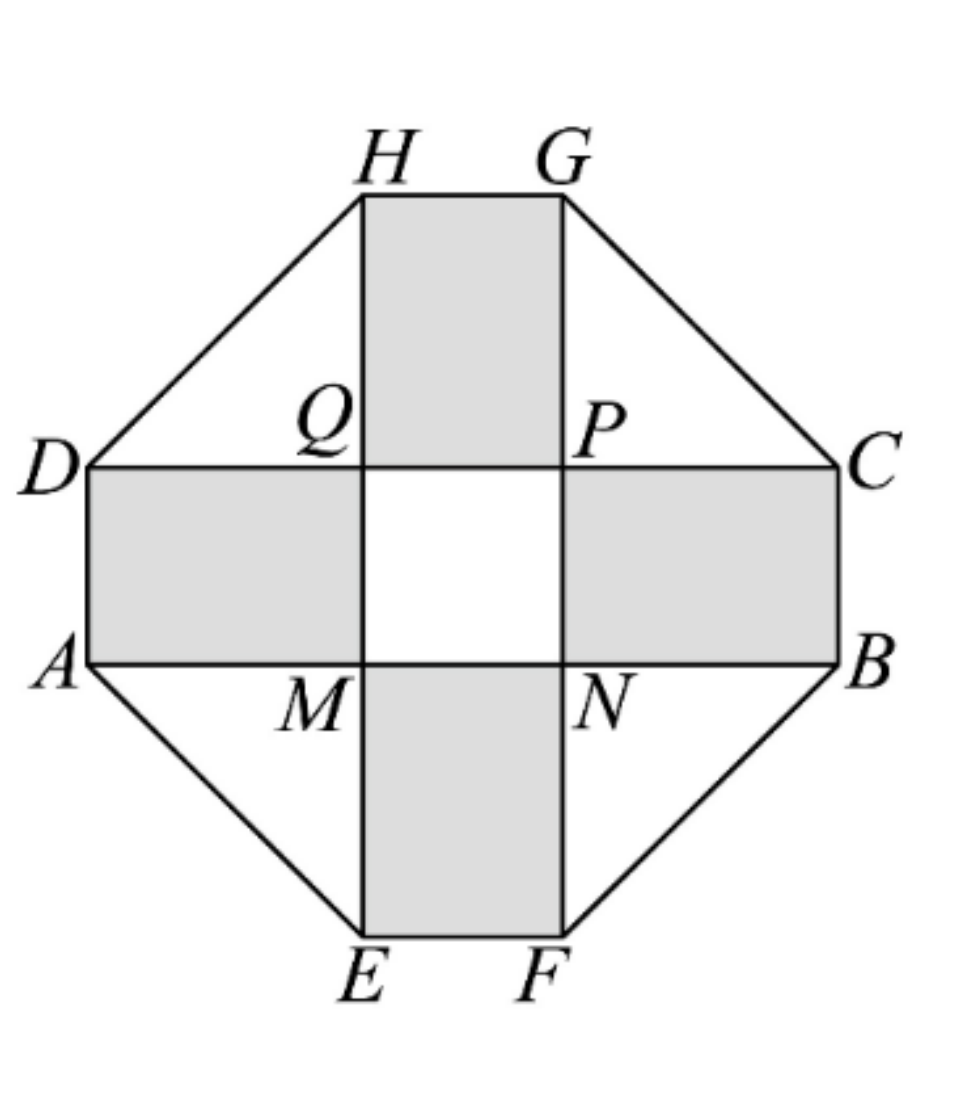
\includegraphics[width=0.34\textwidth]{figures/cross_octagon_h64.png}
\end{center}

\begin{enumerate}[label=(\arabic*)]
\item 设 $DQ$ 长为 $y\mathrm{m}$（$y>0$），用 $x$ 表示 $y$，并求出 $x$ 的取值范围；
\item 如何设计 $AD$ 可使总造价最低，并求出最低造价.
\item 若总造价 $W$ 不超过 69000 元，求 $AD$ 长 $x$ 的取值范围.
\end{enumerate}

\ifanswer
\solbegin
\stepm{(1)}{设 $DQ$ 长为 $y\mathrm{m}$，因为十字形区域面积为 $200\text{m}^2$，}
\step{所以 $4xy+x^2=200$，解得 $y=\dfrac{200-x^2}{4x}=\dfrac{50}{x}-\dfrac x4$；\dots\dots2 分}
\step{因为 $y>0$，所以 $x^2<200$，因为 $x>0$，所以 $0<x<10\sqrt2$.\dots\dots4 分}
\stepm{(2)}{四个矩形地砖面积 $S_{\text{四个矩形}}=4xy=200-x^2$，}
\step{造价 $W_{\text{四个矩形}}=105(200-x^2)$；}
\step{四个三角形草坪面积 $S_{\text{三角形}}=4\times\dfrac12y^2=2\left(\dfrac{50}{x}-\dfrac x4\right)^2=\dfrac{5000}{x^2}+\dfrac{x^2}8-50$，}
\step{造价 $W_{\text{三角形}}=40\left(\dfrac{5000}{x^2}+\dfrac{x^2}8-50\right)$；}
\step{正方形花坛面积 $S_{\text{正方形}}=x^2$，造价 $W_{\text{正方形}}=2100x^2$；}
\step{总造价 $W=W_{\text{四个矩形}}+W_{\text{三角形}}+W_{\text{正方形}}$}
\step{$=105(200-x^2)+40\left(\dfrac{5000}{x^2}+\dfrac{x^2}8-50\right)+2100x^2$，}
\step{化简得 $W=2000x^2+19000+\dfrac{200000}{x^2}$（$0<x<10\sqrt2$）.\dots\dots6 分}
\step{因为 $2000x^2+\dfrac{200000}{x^2}\geqslant40000$，}
\step{当且仅当 $x=\sqrt{10}$（在 $x$ 范围中）时取等号，此时 $W=59000$ 元.}
\step{综上，当 $AD$ 的长为 $\sqrt{10}$ 时，总造价最低，为 59000 元.\dots\dots8 分}
% 原卷 (3) 定义域印作 0<x<2√10，与 (1) 所得 0<x<10√2 不一致，照录（见文件头“原卷笔误”④）
\stepm{(3)}{由（2）得 $W=2000x^2+19000+\dfrac{200000}{x^2}$（$0<x<2\sqrt{10}$）.}
\step{总造价不超过 69000 元，即 $W=2000x^2+19000+\dfrac{200000}{x^2}\leqslant69000$，}
\step{化简得 $x^2+\dfrac{100}{x^2}\leqslant25$，\dots\dots10 分}
\step{即 $(x^2)^2-25x^2+100=(x^2-20)(x^2-5)\leqslant0$，即 $\sqrt5\leqslant x\leqslant2\sqrt5$，}
% 原卷末句“取值范围[√5,2√5]”脱“为”，照录（见文件头“原卷笔误”⑤）
\step{所以 $AD$ 长 $x$ 的取值范围$[\sqrt5,2\sqrt5]$.\dots\dots12 分}
\solend
\fi

\ansspace[10]

\item 设 $a,b,c$ 为实数，集合 $S=\{x\mid(x+a)(x^2+bx+c)=0,x\in\R\}$.

\begin{enumerate}[label=(\arabic*)]
\item 若 $a=1,b=3,c=2$，求集合 $S$；
\item 若 $S=\{-2\}$，求 $a,b,c$ 满足的条件；
\item 设 $T=\{x\mid(ax+1)(cx^2+bx+1)=0,x\in\R\}$，当 $ac\neq0$ 时，如果 $\dfrac12\in S$，$-2\in T$，且
集合 $S,T$ 均恰有两个元素，求三元数对 $(a,b,c)$.
\end{enumerate}

\ifanswer
\solbegin
\stepm{(1)}{若 $a=1,b=3,c=2$，}
\step{则方程 $(x+a)(x^2+bx+c)=0$ 为 $(x+1)(x^2+3x+2)=0$，}
\step{即 $(x+1)^2(x+2)=0$，解得 $x=-1$ 或 $x=-2$，所以 $S=\{-1,-2\}$；}
\stepm{(2)}{由题意得 $-a\in S$，因为 $S=\{-2\}$，所以 $-2$ 是方程 $x+a=0$ 的根，}
\step{即 $-2+a=0$，解得 $a=2$. 由 $S=\{-2\}$，集合 $S$ 有且仅有一个元素，}
\step{即方程 $(x+a)(x^2+bx+c)=0$ 有且仅有一个根，}
\stepm{①}{若 $-2$ 是方程 $x^2+bx+c=0$ 的根，}
\step{则 $\Delta=b^2-4c=0$，且 $-\dfrac b2=-2$，解得 $b=4,c=4$；}
\stepm{②}{若 $-2$ 不是方程 $x^2+bx+c=0$ 的根，则方程 $x^2+bx+c=0$ 无实数根，}
\step{则 $\Delta=b^2-4c<0$，}
\step{综上所述，$\begin{cases}a=2\\ b=4\\ c=4\end{cases}$ 或 $\begin{cases}a=2\\ b^2-4c<0\end{cases}$.}
\stepm{(3)}{$S=\{x\mid(x+a)(x^2+bx+c)=0,x\in\R\}$，}
\step{$T=\{x\mid(ax+1)(cx^2+bx+1)=0,x\in\R\}$，}
\step{由题意得 $a\neq0$ 且 $c\neq0$，则 $-a\in S,-\dfrac1a\in T$，}
\step{且方程 $x^2+bx+c=0$ 与 $cx^2+bx+1=0$ 有相同的判别式 $\Delta=b^2-4c$，}
\step{即两方程根的个数相同. 由集合 $S,T$ 均恰有两个元素，则 $\Delta=b^2-4c\geqslant0$.}
\step{$S=\{x\mid(x+a)(x^2+bx+c)=0,x\in\R\}$，}
\step{因为 $\dfrac12\in S$，所以 $\dfrac12$ 是方程 $x+a=0$ 或 $x^2+bx+c=0$ 的根.}
\step{$T=\{x\mid(ax+1)(cx^2+bx+1)=0,x\in\R\}$，}
\step{由 $-\dfrac1a\in T$，且 $-2\in T$，则 $-2$ 是方程 $ax+1=0$ 或 $cx^2+bx+1=0$ 的根.}
\stepm{①}{当 $a=-\dfrac12$ 时，$\dfrac12$ 是方程 $x+a=0$ 的根，$-a=\dfrac12\in S$，则 $-\dfrac1a=2\in T$，}
\step{又 $-2\in T$，则 $T=\{-2,2\}$，}
\step{由 $T=\left\{x\mid\left(-\dfrac12x+1\right)(cx^2+bx+1)=0,x\in\R\right\}$，}
% 原卷句末为句号，本稿原错作逗号
\step{则 $-2$ 是方程 $cx^2+bx+1=0$ 的根，则 $4c-2b+1=0$.}
\stepm{(i)}{若 $\Delta=b^2-4c=0$，联立 $\begin{cases}4c-2b+1=0\\ b^2-4c=0\end{cases}$ 解得 $b=1,c=\dfrac14$.}
\step{验证：当 $a=-\dfrac12,b=1,c=\dfrac14$ 时，}
\step{$S=\left\{x\mid\left(x-\dfrac12\right)\left(x^2+x+\dfrac14\right)=0,x\in\R\right\}=\left\{-\dfrac12,\dfrac12\right\}$，}
\step{$T=\left\{x\mid\left(-\dfrac12x+1\right)\left(\dfrac14x^2+x+1\right)=0,x\in\R\right\}=\{-2,2\}$，满足题意；}
\stepm{(ii)}{若 $\Delta=b^2-4c>0$，方程 $cx^2+bx+1=0$ 有两个不相等的实数根，}
\step{又 $T=\{-2,2\}$，则方程 $cx^2+bx+1=0$ 的两根必为 $-2$ 和 2.}
\step{由韦达定理得 $\begin{cases}-2+2=-\dfrac bc\\ -2\times2=\dfrac1c\end{cases}$，解得 $b=0,c=-\dfrac14$；}
\step{验证：当 $a=-\dfrac12,b=0,c=-\dfrac14$ 时，}
\step{$S=\left\{x\mid\left(x-\dfrac12\right)\left(x^2-\dfrac14\right)=0,x\in\R\right\}=\left\{-\dfrac12,\dfrac12\right\}$，}
\step{$T=\left\{x\mid\left(-\dfrac12x+1\right)\left(-\dfrac14x^2+1\right)=0,x\in\R\right\}=\{-2,2\}$，满足题意；}
\stepm{②}{当 $a=\dfrac12$ 时，$-\dfrac1a=-2$，即 $-2$ 是方程 $ax+1=0$ 的根，}
\step{则 $-a=-\dfrac12\in S$，又 $\dfrac12\in S$，则 $S=\left\{-\dfrac12,\dfrac12\right\}$，}
\step{$S=\{x\mid(x+a)(x^2+bx+c)=0,x\in\R\}$，}
\step{则 $\dfrac12$ 是方程 $x^2+bx+c=0$ 的根，则 $\dfrac14+\dfrac12b+c=0$，即 $4c+2b+1=0$；}
\stepm{(i)}{若 $\Delta=b^2-4c=0$，联立 $\begin{cases}4c+2b+1=0\\ b^2-4c=0\end{cases}$ 解得 $b=-1,c=\dfrac14$.}
\step{验证：当 $a=\dfrac12,b=-1,c=\dfrac14$ 时，}
\step{$S=\left\{x\mid\left(x+\dfrac12\right)\left(x^2-x+\dfrac14\right)=0,x\in\R\right\}=\left\{-\dfrac12,\dfrac12\right\}$，}
\step{$T=\left\{x\mid\left(\dfrac12x+1\right)\left(\dfrac14x^2-x+1\right)=0,x\in\R\right\}=\{-2,2\}$，满足题意；}
% 原卷作“有两不等的实数根”，本稿原脱“的”
\stepm{(ii)}{若 $\Delta=b^2-4c>0$，方程 $x^2+bx+c=0$ 有两不等的实数根，}
% 原卷句末为句号，本稿原错作逗号
\step{又 $S=\left\{-\dfrac12,\dfrac12\right\}$，则方程 $x^2+bx+c=0$ 的两根必为 $-\dfrac12$ 和 $\dfrac12$.}
\step{由韦达定理得 $\begin{cases}-\dfrac12+\dfrac12=-b\\ -\dfrac12\times\dfrac12=c\end{cases}$，解得 $b=0,c=-\dfrac14$；}
\step{验证：当 $a=\dfrac12,b=0,c=-\dfrac14$ 时，}
\step{$S=\left\{x\mid\left(x+\dfrac12\right)\left(x^2-\dfrac14\right)=0,x\in\R\right\}=\left\{-\dfrac12,\dfrac12\right\}$，}
\step{$T=\left\{x\mid\left(\dfrac12x+1\right)\left(-\dfrac14x^2+1\right)=0,x\in\R\right\}=\{-2,2\}$，满足题意；}
\stepm{③}{当 $a\neq-\dfrac12$ 且 $a\neq\dfrac12$ 时，则 $\dfrac12$ 不是方程 $x+a=0$ 的根，}
\step{$-2$ 也不是方程 $ax+1=0$ 的根.}
% 原卷此句单根而称“两实数根”，语病，照录（见文件头“原卷笔误”⑥）
\step{由 $\dfrac12\in S,-2\in T$，则 $\dfrac12$ 是方程 $x^2+bx+c=0$ 的两实数根，}
\step{且 $-2$ 是方程 $cx^2+bx+1=0$ 的根，则有 $\begin{cases}\dfrac14+\dfrac12b+c=0\\ 4c-2b+1=0\end{cases}$，}
\step{解得 $b=0,c=-\dfrac14$.}
\step{验证：当 $a\neq-\dfrac12$ 且 $a\neq\dfrac12,b=0,c=-\dfrac14$ 时，有 $-a\neq\dfrac12,-a\neq-\dfrac12$.}
\step{$S=\left\{x\mid(x+a)\left(x^2-\dfrac14\right)=0,x\in\R\right\}=\left\{-a,-\dfrac12,\dfrac12\right\}$ 有三个元素，}
\step{故不满足题意；}
\step{综上所述，满足题意的所有三元数对 $(a,b,c)$ 有}
\step{$\left(-\dfrac12,1,\dfrac14\right)$，$\left(-\dfrac12,0,-\dfrac14\right)$，$\left(\dfrac12,-1,\dfrac14\right)$，$\left(\dfrac12,0,-\dfrac14\right)$.}
\solend
\fi

\ansspace*[10]

\end{enumerate}

\end{document}
"
% 紧凑版：xelatex "\def\iscompact{1}% 高一64_格致中学_10月月考.tex
%   —— 高一上数学“2026-2027 年格致中学高一上 10 月月考”（讲评版）
% 试卷版：xelatex 高一64_格致中学_10月月考.tex
% 答案版：xelatex "\def\isanswer{1}\input{高一64_格致中学_10月月考.tex}"
% 紧凑版：xelatex "\def\iscompact{1}\input{高一64_格致中学_10月月考.tex}"
%
% 原始材料：微信公众号“魔都数学加油站”文章，作者破晓，连载“27学年高一64”；
% 原文标题“27学年高一64——2026-2027年上海市格致中学高一上10月月考”；
% 原文链接：https://mp.weixin.qq.com/s/0DfB77nTJf7NdVI_FYXxeA。
% 页面标注发布时间 2026-10-17 21:58（上海）。
% 本次转录只据 `原图/高一64_格致中学_10月月考/` 的 14 张 PNG 逐页读图。
% 正文为 14 张 PNG 页（`01..14.png`）：第 12、13、14 页 2560×3620，
% 第 01—11 页 4762×6735（**同一篇各页分辨率不同**），均按页序读取。
% 14 页全为试卷正文页（卷首标题在第 1 页页顶，卷末解答题第 18 题解析止于第 14 页），
% 无封面页、目录页、二维码或宣传页。粉色斜排“魔都数学加油站”为卷面水印，与公众号页脚一并未录入。
%
% 卷首标题：照卷面印作“2026--2027 年格致中学高一上 10 月月考”，年份区间按全稿惯例排 en dash。
% 原卷只有一行标题、无副标题。
%
% 篇幅与题号：原卷自第 3 题起编号（第 1、2 题不在本卷内）。填空题 3—10（8 题）、
% 选择题 11—14（4 题）、解答题 15—18（4 题），共 16 题。本稿沿用原节与原题号，
% 只改排为全稿统一的大节样式（原卷小节标题为“一、填空题”“二、选择题”“三、解答题”）。
%
% 讲评版：原卷每题下直接印【答案】或【解析】。**只印【答案】的 1 题**（第 5 题），
% 本稿只给 \ans{}；其余 15 题都印【解析】（按全稿口径这类题不另提 \ans{}——第 11、13、14 题
% 的结论写在解析末句（“故选 A”“故选 D”等），亦照录在解析内）。**另有 1 题答案印在题干括号内**——
% 第 12 题（“( B )”，该题无【答案】/【解析】段），本稿按 高一37 第 13 题成例把括号留空、
% 答案另提为 \ans{$B$}。
%
% 副标题：原卷未印副标题。本稿按“知识模块”口径标作“集合与常用逻辑用语、不等式”：
% 16 题中集合与常用逻辑用语 8 题（第 4、9、10、11、12、13、16、18 题），
% 不等式 8 题（含一元二次方程与韦达定理、基本不等式、二次不等式、恒成立、分式不等式：
% 第 3、5、6、7、8、14、15、17 题），两类均达三分之一，故并标。口径同 高一59、高一63。
%
% 与原卷的排版差异：
%   ① 原卷每题下直接印【答案】/【解析】，本稿按全稿惯例将答案与解析置于答案版，试卷版保持干净；
%   ② 原卷未印副标题，本稿按“知识模块”口径补出；
%   ③ 原卷填空横线约三四个字宽，本稿按全稿惯例统一排 \blankline[4.4em]；
%   ④ 原卷实数集排斜体 $R$（第 4、7、8、13、15、18 题）或粗体 $\mathbf{R}$（第 18 题题干与
%      解析共 6 处），整数集排斜体 $Z$（第 9、13 题）或粗体 $\mathbf{Z}$（第 9 题解析末两行），
%      有理数集排粗体 $\mathbf{Q}$（第 13 题选项 A），本稿按全稿惯例统一改用 $\R$、$\Z$、$\Q$
%      （记号归一，粗体／斜体不作区分）；空集记号原卷作 $\varnothing$，照录；
%   ⑤ 第 4 题的补集**原卷用上划线记号 $\bar B$**（题干 1 处、解析 4 处，共 5 处），
%      与全稿惯例的 $\complement_U B$ 不同，本稿照录原卷的 $\bar B$；
%   ⑥ 原卷用描述法时竖线排细竖“$|$”（如 $\{x\mid|x|\geqslant2024\}$ 一类），本稿按全稿惯例排 \mid；
%   ⑦ 第 15—18 题的子问原卷各自另起一行、以“（1）”“（2）”“（3）”标号，本稿按全稿惯例用
%      enumerate 的 (1)(2)(3)；解析中的子问标号一律用 \stepm{(1)}{…}；
%      第 18 题解析中分情形的①②③与分小目的 (i)(ii)，按全稿惯例作 \stepm{①}{…}、\stepm{(i)}{…}；
%   ⑧ 第 13 题解析的“A 选项：”“B 选项：”“C 选项：”“D 选项：”原卷排**加粗**（共 4 处），
%      同 高一63“法一：”成例，本稿排 \stepm{A 选项：}{…} 一类（加粗着色、不改黑色基调），
%      冒号照原卷排全角；
%   ⑨ 第 17 题解析带评分档，原卷在档与档之间排一串点线（“………2 分”），
%      本稿照录为“\dots\dots2 分”一类（同 高一54 成例），共 5 处；
%   ⑩ 选择题的作答括号原卷排半角“(　　)”（第 11、13、14 题括号内空白、第 12 题括号内印 B），
%      本稿按全稿惯例排 \mbox{（\quad）}；选项字母后的句点照原卷排“A.”“B.”；
%   ⑪ 每道解答题原卷未留作答空白，本稿按全稿惯例加 \ansspace（末题用 \ansspace*）；
%   ⑫ 第 17 题题干右侧的十字形八边形示意图，本稿按原卷截图裁出（`figures/cross_octagon_h64.png`，
%      原分辨率裁切，未放大、未用 TikZ 重绘），图内阴影与点名照原卷。
%
% 原卷笔误/存疑（均照录未改，正文对应处另有 % 注）：
%   ① 第 8 题解析末两步自相矛盾：上一步已化为 $\dfrac x{x-1}<0$，下一步却印作
%      “即 $x(x+1)<0$，解得 $-1<x<0$”并给出解集 $(-1,0)$——由 $\dfrac x{x-1}<0$ 应得
%      $x(x-1)<0$、解集 $(0,1)$；已 8 倍放大确认原卷确为 $x+1$ 与 $(-1,0)$，照录未改。
%   ② 第 13 题 D 选项解析“乘法满足结合率”的“率”应为“律”（同段 A、B 选项均作“结合律”）。
%   ③ 第 13 题条件①“任意 $a,b\in G$. 有 $a*b\in G$；”在 $G$ 后印句号（其余三条均以逗号
%      接下文），疑为逗号之误，照录。
%   ④ 第 17 题 (3) 解析把定义域印作 $0<x<2\sqrt{10}$，与 (1) 所得 $0<x<10\sqrt2$ 不一致
%      （疑为 $10\sqrt2$ 之误）；照录未改。
%   ⑤ 第 17 题 (3) 末句“所以 $AD$ 长 $x$ 的取值范围$[\sqrt5,2\sqrt5]$.”脱一个“为”。
%   ⑥ 第 18 题 (3) ③“则 $\dfrac12$ 是方程 $x^2+bx+c=0$ 的**两**实数根”——只有一个数却称
%      “两实数根”，语病；照录。
%
% 插图：第 17 题题干有 1 幅十字形八边形示意图（原卷第 09 页右侧），已按原卷截图排入；
% 其余 13 页无任何图形、无“如图”字样（第 17 题的“图中”均指此图）。
%
\documentclass[a4paper,11pt]{article}
\usepackage{common}

\begin{document}

\examtitlest[3]{2026--2027 年格致中学高一上 10 月月考}{集合与常用逻辑用语、不等式}

\bigsec{一、填空题}

\begin{enumerate}
\setcounter{enumi}{2}

\item 已知一元二次方程 $x^2-nx+5=0$ 的两个实根分别为 $x_1$、$x_2$，且 $\dfrac1{x_1}+\dfrac1{x_2}=1$，则实数 $n$ 的值为\blankline[4.4em].

\ifanswer
\solbegin
\step{$\dfrac1{x_1}+\dfrac1{x_2}=\dfrac{x_1+x_2}{x_1x_2}=\dfrac n5=1$，所以 $n=5$.}
\solend
\fi

\item 全集为 $U=\R$，$A=\{x\mid|x|\geqslant2\}$，$B=\{y\mid y=x^2+1,x\in\R\}$，则 $A\cup\bar B=$\blankline[4.4em].

\ifanswer
\solbegin
\step{由题意得集合 $A=\{x\mid x\geqslant2\text{ 或 }x\leqslant-2\}$，}
\step{因为 $x^2+1\geqslant1$，所以集合 $B=\{x\mid x\geqslant1\}$，所以 $\bar B=\{x\mid x<1\}$，}
\step{则 $A\cup\bar B=\{x\mid x\geqslant2\text{ 或 }x<1\}$.}
\solend
\fi

\item 若 $x>2$，则 $4x+\dfrac1{x-2}$ 的最小值为\blankline[4.4em].

\ifanswer
\ans{$12$}
\fi

\item 已知关于 $x$ 不等式组$\begin{cases}(3x-2)(2x+3)\leqslant0\\ x-a<0\end{cases}$\!没有实数解，则实数 $a$ 的取值范围为\blankline[4.4em].

\ifanswer
\solbegin
\step{由题意得 $\begin{cases}-\dfrac32\leqslant x\leqslant\dfrac23\\ x<a\end{cases}$ 无解，所以 $a\leqslant-\dfrac32$.}
\solend
\fi

\item 若不等式 $\dfrac{x^2-8x+20}{mx^2-mx-1}<0$ 对一切 $x\in\R$ 都成立，则实数 $m$ 的取值范围为\blankline[4.4em].

\ifanswer
\solbegin
\step{因为 $x^2-8x+20=(x-4)^2+4\geqslant4>0$，所以 $mx^2-mx-1<0$，}
\step{当 $m=0$ 时，$mx^2-mx-1=-1<0$，不等式成立；}
\step{设 $y=mx^2-mx-1$，当 $m\neq0$ 时函数 $y$ 为二次函数，$y$ 要恒小于 0，}
\step{抛物线开口向下且与 $x$ 轴没有交点，即 $m<0$ 且 $\Delta<0$，得 $-4<m\leqslant0$，}
\step{故实数 $m$ 的取值范围为 $(-4,0]$.}
\solend
\fi

\item 已知关于 $x$ 的不等式 $\dfrac{ax-1}{x+b}>0$ 的解集为 $\{x\mid-1<x<2\}$，其中 $a$、$b\in\R$，则关于 $x$ 的不等式 $\dfrac{bx+1}{ax+1}<1$ 的解集为\blankline[4.4em].

\ifanswer
\solbegin
\step{不等式 $\dfrac{ax-1}{x+b}>0$ 等价于 $(ax-1)(x+b)>0$，即 $ax^2+(ab-1)x-b>0$，}
\step{所以 $-1$ 和 2 为方程 $ax^2+(ab-1)x-b=0$ 的两根，且 $a<0$，}
\step{由韦达定理得 $\begin{cases}-1+2=-\dfrac{ab-1}a\\ -1\times2=-\dfrac ba\end{cases}$，解得 $\begin{cases}a=-1\\ b=-2\end{cases}$，}
\step{所以原不等式为 $\dfrac{-2x+1}{-x+1}<1\Rightarrow\dfrac{-2x+1}{-x+1}-1<0\Rightarrow\dfrac{-x}{-x+1}<0\Rightarrow\dfrac x{x-1}<0$，}
% 原卷下一步印作“即 x(x+1)<0，解得 -1<x<0”，与上一步 x/(x-1)<0 不等价，
% 照录未改（见文件头“原卷笔误”①）
\step{即 $x(x+1)<0$，解得 $-1<x<0$，即不等式 $\dfrac{bx+1}{ax+1}<1$ 的解集为 $(-1,0)$.}
\solend
\fi

\item 已知集合 $M=\{x\mid|x|\leqslant2024,x\in\Z\}$，集合 $P$ 是 $M$ 的三元子集，即 $P=\{a,b,c\}\subseteq M$，$P$~中元素 $a,b,c$ 满足 $\begin{cases}\dfrac1a+\dfrac1b=\dfrac2c\\ a+c=2b\end{cases}$，则符合要求的集合 $P$ 有\blankline[4.4em]个.

\ifanswer
\solbegin
\step{由 $a+c=2b$，则 $a=2b-c$，代入 $\dfrac1a+\dfrac1b=\dfrac2c$，即 $\dfrac1{2b-c}=\dfrac2c-\dfrac1b=\dfrac{2b-c}{bc}$，}
\step{整理得 $(2b-c)^2=bc$，展开得 $4b^2-5bc+c^2=0$，}
\step{解得 $b=\dfrac c4$ 或 $b=c$（由集合的互异性，舍去），代入 $a+c=2b$ 得 $a=-\dfrac c2$，}
\step{则 $P=\left\{-\dfrac c2,\dfrac c4,c\right\}\subseteq\{x\mid-2024\leqslant x\leqslant2024,x\in\Z\}$，所以 $c$ 为 4 的整数倍，}
\step{且不为 0，则共有 $\dfrac{2024}4\times2=1012$ 个.}
\solend
\fi

\item 已知正整数 $n\geqslant2$，对集合 $\{1,2,3,\cdots,n\}$ 及其每一个非空子集 $X$，记
$X=\{x_1,x_2,\cdots,x_k\}$，其中 $x_1>x_2>\cdots>x_k$，定义一个运算“交替和”
$S_X=x_1-x_2+x_3\cdots+(-1)^{k+1}x_k$. 例如：对于集合 $X=\{9,6,4,2,1\}$，
$S_X=9-6+4-2+1=6$. 则当 $n=7$ 时，集合 $\{1,2,3,\cdots,n\}$ 的所有子集的“交替和”的总
和为\blankline[4.4em].

\ifanswer
\solbegin
\step{由题意得集合 $\{7\}$ 的“交替和”为 7.}
\step{集合 $\{1,2,3,4,5,6,7\}$ 的所有 $2^7$ 个子集中，除去集合 $\{7\}$ 外，}
\step{还有 $2^7-2$ 个非空子集，这 $2^7-2$ 个非空子集中不含元素 7 的集合，}
\step{即 $\{1,2,3,4,5,6\}$ 的非空子集，共有 $2^6-1$ 个，设为 $A_i(i=1,2,\cdots,2^6-1)$；}
\step{则这 $2^7-2$ 个非空子集中含元素 7 的集合，也共有 $2^6-1$ 个，}
\step{这样的集合都可以看成相应地在每个不含 7 的集合中再加上元素 7 得到，}
\step{即 $A_i\cup\{7\}$.}
\step{对 $A_i(i=1,2,\cdots,2^6-1)$ 中的任意集合 $A$，记 $A=\{x_1,x_2,\cdots,x_k\}$，}
\step{则“交替和”$S_A=x_1-x_2+x_3\cdots+(-1)^{k+1}x_k$，其中 $x_1>x_2>\cdots>x_k$，}
\step{由 $7>x_1>x_2>\cdots>x_k$，}
\step{则集合 $A\cup\{7\}$ 的“交替和”为 $7-[x_1-x_2+x_3\cdots+(-1)^{k+1}x_k]$，}
\step{则集合 $A$ 与集合 $A\cup\{7\}$ 的“交替和”之和为 7，下面举例说明：}
\step{如集合 $\{6,5,4,3,2,1\}$ 与集合 $\{7,6,5,4,3,2,1\}$，}
\step{$\{6,5,4,3,2,1\}$ 的“交替和”为 $6-5+4-3+2-1=3$，}
% 原卷此句在页末折为两个印刷行（“……的“交替和”为”／“7-6+5-4+3-2+1=……”），
% 本稿原并作一条，现照原卷拆开（原卷原样两行 / 本稿原错处：并作一行）
\step{$\{7,6,5,4,3,2,1\}$ 的“交替和”为}
\step{$7-6+5-4+3-2+1=7-(6-5+4-3+2-1)=7-3$，}
\step{即集合 $\{6,5,4,3,2,1\}$ 与集合 $\{7,6,5,4,3,2,1\}$ 的“交替和”之和为 7.}
\step{综上，把这 $2^7-2$ 个非空子集两两结组后分别计算每一组中“交替和”之和，}
\step{且每组中“交替和”之和都为 7，共有 $2^6-1$ 组.}
\step{故集合 $\{1,2,3,4,5,6,7\}$ 所有“交替和”之和，}
\step{由各组之和再加集合 $\{7\}$ 的“交替和”7 即可，}
\step{综上所述，当 $n=7$ 时，集合 $\{1,2,3,\cdots,n\}$ 的所有子集的所有“交替和”之和}
\step{为 $7\times(2^6-1)+7=448$.}
\solend
\fi

\end{enumerate}

\bigsec{二、选择题}

\begin{enumerate}
\setcounter{enumi}{10}

\item 若 $a$、$b\in\R$，则“$a<b<0$”是“$a^2>b^2$”的\mbox{（\quad）}条件.

\keepwithprev
A. 充分非必要\qquad B. 必要非充分

C. 充要\qquad D. 既非充分也非必要

\ifanswer
\solbegin
\step{由 $a<b<0\Rightarrow-a>-b>0\Rightarrow(-a)^2>(-b)^2\Rightarrow a^2>b^2$，}
\step{因此由 $a<b<0$ 可以推出 $a^2>b^2$，}
\step{但是当 $a=1$，$b=0$ 时，显然 $a^2>b^2$ 成立，但是 $a<b<0$ 不成立，}
\step{因此由 $a^2>b^2$ 不一定能推出 $a<b<0$，}
\step{因此“$a<b<0$”是“$a^2>b^2$”的充分非必要条件. 故选 $A$.}
\solend
\fi

% 第 12 题答案“B”直接印在题干括号内“(  B  )”，且该题无【答案】/【解析】段；
% 按 高一37 第 13 题的成例括号留空、答案另提为 \ans{}（见文件头）
\item 用反证法证明结论“$a$、$b$、$c$ 至少有一个是正数”时，应假设\mbox{（\quad）}

\keepwithprev
A. $a$、$b$、$c$ 都是正数\qquad B. $a$、$b$、$c$ 都不是正数

C. $a$、$b$、$c$ 至多有一个正数\qquad D. $a$、$b$、$c$ 至多有两个正数

\ifanswer
\ans{$B$}
\fi

\item “群”的概念由数学家伽罗瓦在 19 世纪 30 年代开创，群论虽起源于对代数多项式方程
的研究，但在量子力学、晶体结构学等其他学科中也有十分广泛的应用.“群”的定义是：

设 $G$ 为某种元素组成的一个非空集合，若在 $G$ 内定义一个运算“*”，满足以下条件：

% 原卷条件①在 G 后印句号，疑为逗号之误，照录（见文件头“原卷笔误”③）
①任意 $a,b\in G$. 有 $a*b\in G$；

②如 $a,b,c\in G$，有 $(a*b)*c=a*(b*c)$；

③在 $G$ 中有一个元素 $e$，对任意 $a\in G$，都有 $a*e=e*a=a$，称 $e$ 为 $G$ 的单位元；

④任意 $a\in G$，在 $G$ 中存在唯一确定的 $b$，使 $a*b=b*a=e$，称 $b$ 为 $a$ 的逆元；

此时称 $(G,*)$ 为一个群.

例如实数集 $\R$ 和实数集上的加法运算“+”就构成一个群 $(\R,+)$，其单位元是 0，每一个数
的逆元是其相反数，那么下列说法中，错误的是\mbox{（\quad）}

\keepwithprev
A. $G=\Q$，则 $(G,+)$ 为一个群

B. $G=\{\sqrt2m+\sqrt3n\mid m,n\in\Z\}$，$(G,+)$ 为一个群

C. $G=\{-1,1\}$，则 $(G,\times)$ 为一个群

D. $G=\{x\mid x=2k+1,k\in\Z\}$，则 $(G,\times)$ 为一个群

\ifanswer
\solbegin
\stepm{A 选项：}{有理数的和还是有理数，求和满足结合律，}
\step{设 $a\in\Q$，单位元为 $e$，则 $a+e=a$，故 $e=0$，}
\step{所以每一个数的相反数为其逆元，故 $(G,+)$ 为一个群，选项 A 正确；}
\stepm{B 选项：}{$G=\{\sqrt2m+\sqrt3n\mid m,n\in\Z\}$ 中的任何两个数相加还是属于}
\step{$G=\{\sqrt2m+\sqrt3n\mid m,n\in\Z\}$，求和满足结合律，}
\step{设 $\sqrt2x+\sqrt3y\in G,x,y\in\Z$，单位元为 $e$，}
\step{则 $\sqrt2x+\sqrt3y+e=\sqrt2x+\sqrt3y$，所以 $e=0$，}
\step{每一个数的相反数为其逆元，$(G,+)$ 为一个群，选项 B 正确；}
\stepm{C 选项：}{$G=\{-1,1\}$ 中的两个元素相乘，其积可能为 1 或 $-1$，又 $1\in G,-1\in G$，}
\step{设 $a\in G$，单位元为 $e$，则 $a\times e=a$，故 $e=1,1$ 的逆元为 $1,-1$ 的逆元为 $-1$，}
\step{所以 $(G,\times)$ 为一个群，选项 C 正确；}
% 原卷“乘法满足结合率”的“率”应为“律”（同段 A、B 选项均作“结合律”），照录（见文件头“原卷笔误”②）
\stepm{D 选项：}{两个奇数相乘还是奇数，乘法满足结合率，}
\step{设 $a\in G$，单位元为 $e$，则 $a\times e=a$，故 $e=1$，}
\step{又 $3\in G$，故存在 $b\in G$，使得 $3b=1$，则 $b=\dfrac13$，矛盾，}
\step{故 $(G,\times)$ 不为一个群，选项 D 错误.}
\step{故选 $D$.}
\solend
\fi

\item 已知 $a$、$b$、$c\in\R$，若关于 $x$ 的不等式 $0\leqslant x+\dfrac ax+b\leqslant\dfrac cx-1$ 的解集为 $[x_1,x_2]\cup\{x_3\}$
（$x_3>x_2>x_1>0$），则\mbox{（\quad）}

\keepwithprev
A. 不存在有序数组 $(a,b,c)$，使得 $x_2-x_1=1$

B. 存在唯一有序数组 $(a,b,c)$，使得 $x_2-x_1=1$

C. 有且只有两组有序数组 $(a,b,c)$，使得 $x_2-x_1=1$

D. 存在无穷多组有序数组 $(a,b,c)$，使得 $x_2-x_1=1$

\ifanswer
\solbegin
\step{因为不等式 $0\leqslant x+\dfrac ax+b\leqslant\dfrac cx-1$ 的解集为 $[x_1,x_2]\cup\{x_3\}$（$x_3>x_2>x_1>0$），}
\step{所以 $0\leqslant x^2+bx+a\leqslant c-x$ 在 $[x_1,x_2]\cup\{x_3\}$ 上成立，}
\step{假设 $x_1=m$，$x_2=m+1$，$x_3=n$，}
\step{则 $c-n=0=n^2+bn+a$，由 $x_3$ 为一个独立的数得出，}
\step{所以 $n=c$，且 $m+1$ 与 $n$ 为方程 $x^2+bx+a=0$ 的两个根，}
\step{因为 $x_3>x_2>x_1>0$，所以 $-b=m+n+1=m+c+1$，$a=mn+n=mc+c$，}
\step{所以 $b=-m-c-1$，}
\step{且点 $(x_1,x_1^2+bx_1+a)$ 为 $y=x^2+bx+a$ 与 $y=c-x$ 的左交点，}
\step{所以 $m^2+bm+a=c-m$ 且 $b=-m-c-1$，$a=mc+c$，}
\step{故 $m^2+bm+a=m^2-m^2-mc-m+mc+c=c-m$，所以 $c-m=c-m$ 恒成立，}
\step{所以不论 $a$、$b$、$c$ 取何值，$x_2-x_1=1$ 恒成立，}
\step{即存在无穷多组有序数组 $(a,b,c)$，使得 $x_2-x_1=1$，}
\step{故选项 $A$、$B$、$C$ 错误，选项 $D$ 正确. 故选 $D$.}
\solend
\fi

\end{enumerate}

\bigsec{三、解答题}

\begin{enumerate}
\setcounter{enumi}{14}

\item 已知函数 $f(x)=(a-1)x^2-ax+1$，$a\in\R$.

\begin{enumerate}[label=(\arabic*)]
\item 若不等式 $f(x)<0$ 的解集为 $\left(\dfrac13,1\right)$，求实数 $a$ 的值；
\item 当 $a>1$ 时，解关于 $x$ 的不等式 $f(x)\geqslant0$.
\end{enumerate}

\ifanswer
\solbegin
\stepm{(1)}{因为不等式 $f(x)<0$ 的解集为 $\left(\dfrac13,1\right)$，}
\step{所以不等式对应的方程 $(a-1)x^2-ax+1=0$ 的两根分别为 $\dfrac13$、1，}
\step{由根与系数的关系得 $\begin{cases}1+\dfrac13=\dfrac a{a-1}\\ 1\times\dfrac13=\dfrac1{a-1}\end{cases}$，解得 $a=4$；}
\stepm{(2)}{不等式 $(a-1)x^2-ax+1\geqslant0$（$a>1$）可化为 $(x-1)[(a-1)x-1]\geqslant0$，}
\step{不等式对应方程的两根为 $x_1=1$，$x_2=\dfrac1{a-1}$，}
\step{①当 $\dfrac1{a-1}=1$，即 $a=2$ 时，不等式为 $(x-1)^2\geqslant0$，解集为 $\R$；}
\step{②当 $\dfrac1{a-1}>1$，即 $1<a<2$ 时，解不等式得 $x\leqslant1$ 或 $x\geqslant\dfrac1{a-1}$；}
\step{③当 $\dfrac1{a-1}<1$，即 $a>2$ 时，解不等式得 $x\leqslant\dfrac1{a-1}$ 或 $x\geqslant1$；}
\step{综上，$a=2$ 时，不等式的解集为 $\R$，}
\step{$1<a<2$ 时，不等式的解集为 $(-\infty,1]\cup\left[\dfrac1{a-1},+\infty\right)$，}
\step{$a>2$ 时，不等式的解集为 $\left(-\infty,\dfrac1{a-1}\right]\cup[1,+\infty)$.}
\solend
\fi

\ansspace[6]

\item 若集合 $A=\{x\mid x^2+5x-6=0\}$，$B=\{x\mid x^2+2(m+1)x+m^2-3=0\}$.

\begin{enumerate}[label=(\arabic*)]
\item 若 $m=0$，写出 $A\cup B$ 的子集个数；
\item 若 $A\cap B=B$，求实数 $m$ 的取值范围.
\end{enumerate}

\ifanswer
\solbegin
\stepm{(1)}{当 $m=0$ 时，$B=\{1,-3\}$，}
\step{因为 $A=\{x\mid x^2+5x-6=0\}=\{-6,1\}$，}
\step{所以 $A\cup B=\{-6,-3,1\}$，集合元素个数为 3 个，}
\step{故 $A\cup B$ 的子集个数为 $2^3=8$.}
\stepm{(2)}{因为 $A\cap B=B$，所以 $B\subseteq A$，}
\step{$\Delta=4(m+1)^2-4(m^2-3)=8m+16$，}
\step{当 $\Delta<0$，即 $m<-2$ 时，$B=\varnothing$，符合题意，}
\step{当 $\Delta=0$，即 $m=-2$ 时，$B=\{1\}$，符合题意，}
\step{当 $\Delta>0$，即 $m>-2$ 时，若 $B\subseteq A$，则 $B=\{-6,1\}$，}
\step{即 $\begin{cases}-2(m+1)=-5\\ m^2-3=-6\end{cases}$，方程组无解，}
\step{综上所述，$m$ 的取值范围为 $(-\infty,-2]$.}
\solend
\fi

\ansspace[6]

\item 2025 年上海奇迹花园国际艺术花展于 9 月 20 日正式启幕，本次花展首次实现沉浸 IP
展、花卉景观、跨界艺术、光影夜花园四展合一，为市民游客打造一个可游、可赏、可感
的秋季治愈系童话世界. 某公园受此启发打算设计一个八边形活动区域，该区域的主体造
型平面图是由两个相同的矩形 $ABCD$ 和 $EFGH$ 构成的十字形地域，十字形的面积为
$200\text{m}^2$. 计划在正方形 $MNPQ$ 上建一座花坛，造价为 2100 元$/\text{m}^2$；在四个相同的矩形
（图中阴影部分）上铺地砖，造价为 105 元$/\text{m}^2$；再在四个空角（图中四个三角
形）上铺草坪，造价为 40 元$/\text{m}^2$. 设 $AD$ 长为 $x\mathrm{m}$（$x>0$），总造价为 $W$ 元，求：

\begin{center}
% 插图取自原卷第 09 页右侧截图（原分辨率裁切，未用 TikZ 重绘），阴影与点名照原卷
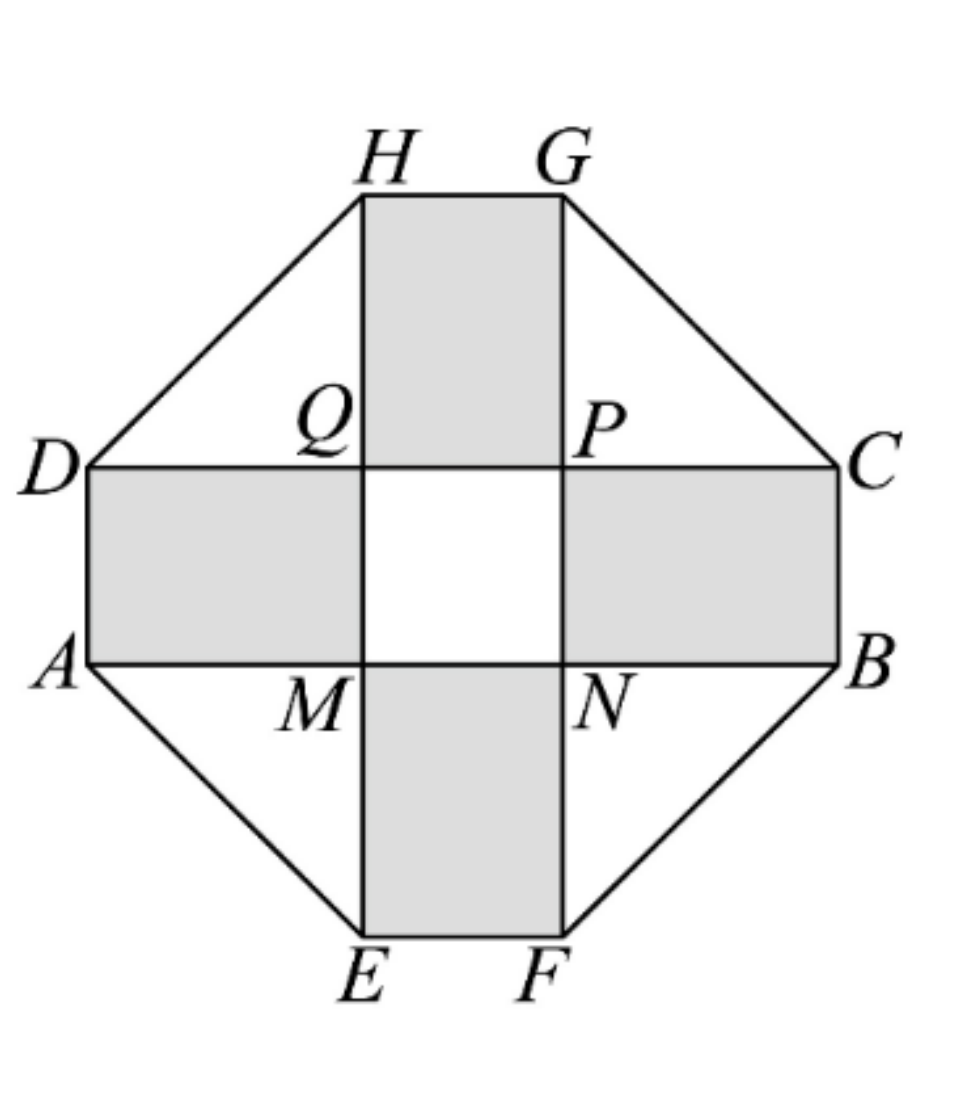
\includegraphics[width=0.34\textwidth]{figures/cross_octagon_h64.png}
\end{center}

\begin{enumerate}[label=(\arabic*)]
\item 设 $DQ$ 长为 $y\mathrm{m}$（$y>0$），用 $x$ 表示 $y$，并求出 $x$ 的取值范围；
\item 如何设计 $AD$ 可使总造价最低，并求出最低造价.
\item 若总造价 $W$ 不超过 69000 元，求 $AD$ 长 $x$ 的取值范围.
\end{enumerate}

\ifanswer
\solbegin
\stepm{(1)}{设 $DQ$ 长为 $y\mathrm{m}$，因为十字形区域面积为 $200\text{m}^2$，}
\step{所以 $4xy+x^2=200$，解得 $y=\dfrac{200-x^2}{4x}=\dfrac{50}{x}-\dfrac x4$；\dots\dots2 分}
\step{因为 $y>0$，所以 $x^2<200$，因为 $x>0$，所以 $0<x<10\sqrt2$.\dots\dots4 分}
\stepm{(2)}{四个矩形地砖面积 $S_{\text{四个矩形}}=4xy=200-x^2$，}
\step{造价 $W_{\text{四个矩形}}=105(200-x^2)$；}
\step{四个三角形草坪面积 $S_{\text{三角形}}=4\times\dfrac12y^2=2\left(\dfrac{50}{x}-\dfrac x4\right)^2=\dfrac{5000}{x^2}+\dfrac{x^2}8-50$，}
\step{造价 $W_{\text{三角形}}=40\left(\dfrac{5000}{x^2}+\dfrac{x^2}8-50\right)$；}
\step{正方形花坛面积 $S_{\text{正方形}}=x^2$，造价 $W_{\text{正方形}}=2100x^2$；}
\step{总造价 $W=W_{\text{四个矩形}}+W_{\text{三角形}}+W_{\text{正方形}}$}
\step{$=105(200-x^2)+40\left(\dfrac{5000}{x^2}+\dfrac{x^2}8-50\right)+2100x^2$，}
\step{化简得 $W=2000x^2+19000+\dfrac{200000}{x^2}$（$0<x<10\sqrt2$）.\dots\dots6 分}
\step{因为 $2000x^2+\dfrac{200000}{x^2}\geqslant40000$，}
\step{当且仅当 $x=\sqrt{10}$（在 $x$ 范围中）时取等号，此时 $W=59000$ 元.}
\step{综上，当 $AD$ 的长为 $\sqrt{10}$ 时，总造价最低，为 59000 元.\dots\dots8 分}
% 原卷 (3) 定义域印作 0<x<2√10，与 (1) 所得 0<x<10√2 不一致，照录（见文件头“原卷笔误”④）
\stepm{(3)}{由（2）得 $W=2000x^2+19000+\dfrac{200000}{x^2}$（$0<x<2\sqrt{10}$）.}
\step{总造价不超过 69000 元，即 $W=2000x^2+19000+\dfrac{200000}{x^2}\leqslant69000$，}
\step{化简得 $x^2+\dfrac{100}{x^2}\leqslant25$，\dots\dots10 分}
\step{即 $(x^2)^2-25x^2+100=(x^2-20)(x^2-5)\leqslant0$，即 $\sqrt5\leqslant x\leqslant2\sqrt5$，}
% 原卷末句“取值范围[√5,2√5]”脱“为”，照录（见文件头“原卷笔误”⑤）
\step{所以 $AD$ 长 $x$ 的取值范围$[\sqrt5,2\sqrt5]$.\dots\dots12 分}
\solend
\fi

\ansspace[10]

\item 设 $a,b,c$ 为实数，集合 $S=\{x\mid(x+a)(x^2+bx+c)=0,x\in\R\}$.

\begin{enumerate}[label=(\arabic*)]
\item 若 $a=1,b=3,c=2$，求集合 $S$；
\item 若 $S=\{-2\}$，求 $a,b,c$ 满足的条件；
\item 设 $T=\{x\mid(ax+1)(cx^2+bx+1)=0,x\in\R\}$，当 $ac\neq0$ 时，如果 $\dfrac12\in S$，$-2\in T$，且
集合 $S,T$ 均恰有两个元素，求三元数对 $(a,b,c)$.
\end{enumerate}

\ifanswer
\solbegin
\stepm{(1)}{若 $a=1,b=3,c=2$，}
\step{则方程 $(x+a)(x^2+bx+c)=0$ 为 $(x+1)(x^2+3x+2)=0$，}
\step{即 $(x+1)^2(x+2)=0$，解得 $x=-1$ 或 $x=-2$，所以 $S=\{-1,-2\}$；}
\stepm{(2)}{由题意得 $-a\in S$，因为 $S=\{-2\}$，所以 $-2$ 是方程 $x+a=0$ 的根，}
\step{即 $-2+a=0$，解得 $a=2$. 由 $S=\{-2\}$，集合 $S$ 有且仅有一个元素，}
\step{即方程 $(x+a)(x^2+bx+c)=0$ 有且仅有一个根，}
\stepm{①}{若 $-2$ 是方程 $x^2+bx+c=0$ 的根，}
\step{则 $\Delta=b^2-4c=0$，且 $-\dfrac b2=-2$，解得 $b=4,c=4$；}
\stepm{②}{若 $-2$ 不是方程 $x^2+bx+c=0$ 的根，则方程 $x^2+bx+c=0$ 无实数根，}
\step{则 $\Delta=b^2-4c<0$，}
\step{综上所述，$\begin{cases}a=2\\ b=4\\ c=4\end{cases}$ 或 $\begin{cases}a=2\\ b^2-4c<0\end{cases}$.}
\stepm{(3)}{$S=\{x\mid(x+a)(x^2+bx+c)=0,x\in\R\}$，}
\step{$T=\{x\mid(ax+1)(cx^2+bx+1)=0,x\in\R\}$，}
\step{由题意得 $a\neq0$ 且 $c\neq0$，则 $-a\in S,-\dfrac1a\in T$，}
\step{且方程 $x^2+bx+c=0$ 与 $cx^2+bx+1=0$ 有相同的判别式 $\Delta=b^2-4c$，}
\step{即两方程根的个数相同. 由集合 $S,T$ 均恰有两个元素，则 $\Delta=b^2-4c\geqslant0$.}
\step{$S=\{x\mid(x+a)(x^2+bx+c)=0,x\in\R\}$，}
\step{因为 $\dfrac12\in S$，所以 $\dfrac12$ 是方程 $x+a=0$ 或 $x^2+bx+c=0$ 的根.}
\step{$T=\{x\mid(ax+1)(cx^2+bx+1)=0,x\in\R\}$，}
\step{由 $-\dfrac1a\in T$，且 $-2\in T$，则 $-2$ 是方程 $ax+1=0$ 或 $cx^2+bx+1=0$ 的根.}
\stepm{①}{当 $a=-\dfrac12$ 时，$\dfrac12$ 是方程 $x+a=0$ 的根，$-a=\dfrac12\in S$，则 $-\dfrac1a=2\in T$，}
\step{又 $-2\in T$，则 $T=\{-2,2\}$，}
\step{由 $T=\left\{x\mid\left(-\dfrac12x+1\right)(cx^2+bx+1)=0,x\in\R\right\}$，}
% 原卷句末为句号，本稿原错作逗号
\step{则 $-2$ 是方程 $cx^2+bx+1=0$ 的根，则 $4c-2b+1=0$.}
\stepm{(i)}{若 $\Delta=b^2-4c=0$，联立 $\begin{cases}4c-2b+1=0\\ b^2-4c=0\end{cases}$ 解得 $b=1,c=\dfrac14$.}
\step{验证：当 $a=-\dfrac12,b=1,c=\dfrac14$ 时，}
\step{$S=\left\{x\mid\left(x-\dfrac12\right)\left(x^2+x+\dfrac14\right)=0,x\in\R\right\}=\left\{-\dfrac12,\dfrac12\right\}$，}
\step{$T=\left\{x\mid\left(-\dfrac12x+1\right)\left(\dfrac14x^2+x+1\right)=0,x\in\R\right\}=\{-2,2\}$，满足题意；}
\stepm{(ii)}{若 $\Delta=b^2-4c>0$，方程 $cx^2+bx+1=0$ 有两个不相等的实数根，}
\step{又 $T=\{-2,2\}$，则方程 $cx^2+bx+1=0$ 的两根必为 $-2$ 和 2.}
\step{由韦达定理得 $\begin{cases}-2+2=-\dfrac bc\\ -2\times2=\dfrac1c\end{cases}$，解得 $b=0,c=-\dfrac14$；}
\step{验证：当 $a=-\dfrac12,b=0,c=-\dfrac14$ 时，}
\step{$S=\left\{x\mid\left(x-\dfrac12\right)\left(x^2-\dfrac14\right)=0,x\in\R\right\}=\left\{-\dfrac12,\dfrac12\right\}$，}
\step{$T=\left\{x\mid\left(-\dfrac12x+1\right)\left(-\dfrac14x^2+1\right)=0,x\in\R\right\}=\{-2,2\}$，满足题意；}
\stepm{②}{当 $a=\dfrac12$ 时，$-\dfrac1a=-2$，即 $-2$ 是方程 $ax+1=0$ 的根，}
\step{则 $-a=-\dfrac12\in S$，又 $\dfrac12\in S$，则 $S=\left\{-\dfrac12,\dfrac12\right\}$，}
\step{$S=\{x\mid(x+a)(x^2+bx+c)=0,x\in\R\}$，}
\step{则 $\dfrac12$ 是方程 $x^2+bx+c=0$ 的根，则 $\dfrac14+\dfrac12b+c=0$，即 $4c+2b+1=0$；}
\stepm{(i)}{若 $\Delta=b^2-4c=0$，联立 $\begin{cases}4c+2b+1=0\\ b^2-4c=0\end{cases}$ 解得 $b=-1,c=\dfrac14$.}
\step{验证：当 $a=\dfrac12,b=-1,c=\dfrac14$ 时，}
\step{$S=\left\{x\mid\left(x+\dfrac12\right)\left(x^2-x+\dfrac14\right)=0,x\in\R\right\}=\left\{-\dfrac12,\dfrac12\right\}$，}
\step{$T=\left\{x\mid\left(\dfrac12x+1\right)\left(\dfrac14x^2-x+1\right)=0,x\in\R\right\}=\{-2,2\}$，满足题意；}
% 原卷作“有两不等的实数根”，本稿原脱“的”
\stepm{(ii)}{若 $\Delta=b^2-4c>0$，方程 $x^2+bx+c=0$ 有两不等的实数根，}
% 原卷句末为句号，本稿原错作逗号
\step{又 $S=\left\{-\dfrac12,\dfrac12\right\}$，则方程 $x^2+bx+c=0$ 的两根必为 $-\dfrac12$ 和 $\dfrac12$.}
\step{由韦达定理得 $\begin{cases}-\dfrac12+\dfrac12=-b\\ -\dfrac12\times\dfrac12=c\end{cases}$，解得 $b=0,c=-\dfrac14$；}
\step{验证：当 $a=\dfrac12,b=0,c=-\dfrac14$ 时，}
\step{$S=\left\{x\mid\left(x+\dfrac12\right)\left(x^2-\dfrac14\right)=0,x\in\R\right\}=\left\{-\dfrac12,\dfrac12\right\}$，}
\step{$T=\left\{x\mid\left(\dfrac12x+1\right)\left(-\dfrac14x^2+1\right)=0,x\in\R\right\}=\{-2,2\}$，满足题意；}
\stepm{③}{当 $a\neq-\dfrac12$ 且 $a\neq\dfrac12$ 时，则 $\dfrac12$ 不是方程 $x+a=0$ 的根，}
\step{$-2$ 也不是方程 $ax+1=0$ 的根.}
% 原卷此句单根而称“两实数根”，语病，照录（见文件头“原卷笔误”⑥）
\step{由 $\dfrac12\in S,-2\in T$，则 $\dfrac12$ 是方程 $x^2+bx+c=0$ 的两实数根，}
\step{且 $-2$ 是方程 $cx^2+bx+1=0$ 的根，则有 $\begin{cases}\dfrac14+\dfrac12b+c=0\\ 4c-2b+1=0\end{cases}$，}
\step{解得 $b=0,c=-\dfrac14$.}
\step{验证：当 $a\neq-\dfrac12$ 且 $a\neq\dfrac12,b=0,c=-\dfrac14$ 时，有 $-a\neq\dfrac12,-a\neq-\dfrac12$.}
\step{$S=\left\{x\mid(x+a)\left(x^2-\dfrac14\right)=0,x\in\R\right\}=\left\{-a,-\dfrac12,\dfrac12\right\}$ 有三个元素，}
\step{故不满足题意；}
\step{综上所述，满足题意的所有三元数对 $(a,b,c)$ 有}
\step{$\left(-\dfrac12,1,\dfrac14\right)$，$\left(-\dfrac12,0,-\dfrac14\right)$，$\left(\dfrac12,-1,\dfrac14\right)$，$\left(\dfrac12,0,-\dfrac14\right)$.}
\solend
\fi

\ansspace*[10]

\end{enumerate}

\end{document}
"
%
% 原始材料：微信公众号“魔都数学加油站”文章，作者破晓，连载“27学年高一64”；
% 原文标题“27学年高一64——2026-2027年上海市格致中学高一上10月月考”；
% 原文链接：https://mp.weixin.qq.com/s/0DfB77nTJf7NdVI_FYXxeA。
% 页面标注发布时间 2026-10-17 21:58（上海）。
% 本次转录只据 `原图/高一64_格致中学_10月月考/` 的 14 张 PNG 逐页读图。
% 正文为 14 张 PNG 页（`01..14.png`）：第 12、13、14 页 2560×3620，
% 第 01—11 页 4762×6735（**同一篇各页分辨率不同**），均按页序读取。
% 14 页全为试卷正文页（卷首标题在第 1 页页顶，卷末解答题第 18 题解析止于第 14 页），
% 无封面页、目录页、二维码或宣传页。粉色斜排“魔都数学加油站”为卷面水印，与公众号页脚一并未录入。
%
% 卷首标题：照卷面印作“2026--2027 年格致中学高一上 10 月月考”，年份区间按全稿惯例排 en dash。
% 原卷只有一行标题、无副标题。
%
% 篇幅与题号：原卷自第 3 题起编号（第 1、2 题不在本卷内）。填空题 3—10（8 题）、
% 选择题 11—14（4 题）、解答题 15—18（4 题），共 16 题。本稿沿用原节与原题号，
% 只改排为全稿统一的大节样式（原卷小节标题为“一、填空题”“二、选择题”“三、解答题”）。
%
% 讲评版：原卷每题下直接印【答案】或【解析】。**只印【答案】的 1 题**（第 5 题），
% 本稿只给 \ans{}；其余 15 题都印【解析】（按全稿口径这类题不另提 \ans{}——第 11、13、14 题
% 的结论写在解析末句（“故选 A”“故选 D”等），亦照录在解析内）。**另有 1 题答案印在题干括号内**——
% 第 12 题（“( B )”，该题无【答案】/【解析】段），本稿按 高一37 第 13 题成例把括号留空、
% 答案另提为 \ans{$B$}。
%
% 副标题：原卷未印副标题。本稿按“知识模块”口径标作“集合与常用逻辑用语、不等式”：
% 16 题中集合与常用逻辑用语 8 题（第 4、9、10、11、12、13、16、18 题），
% 不等式 8 题（含一元二次方程与韦达定理、基本不等式、二次不等式、恒成立、分式不等式：
% 第 3、5、6、7、8、14、15、17 题），两类均达三分之一，故并标。口径同 高一59、高一63。
%
% 与原卷的排版差异：
%   ① 原卷每题下直接印【答案】/【解析】，本稿按全稿惯例将答案与解析置于答案版，试卷版保持干净；
%   ② 原卷未印副标题，本稿按“知识模块”口径补出；
%   ③ 原卷填空横线约三四个字宽，本稿按全稿惯例统一排 \blankline[4.4em]；
%   ④ 原卷实数集排斜体 $R$（第 4、7、8、13、15、18 题）或粗体 $\mathbf{R}$（第 18 题题干与
%      解析共 6 处），整数集排斜体 $Z$（第 9、13 题）或粗体 $\mathbf{Z}$（第 9 题解析末两行），
%      有理数集排粗体 $\mathbf{Q}$（第 13 题选项 A），本稿按全稿惯例统一改用 $\R$、$\Z$、$\Q$
%      （记号归一，粗体／斜体不作区分）；空集记号原卷作 $\varnothing$，照录；
%   ⑤ 第 4 题的补集**原卷用上划线记号 $\bar B$**（题干 1 处、解析 4 处，共 5 处），
%      与全稿惯例的 $\complement_U B$ 不同，本稿照录原卷的 $\bar B$；
%   ⑥ 原卷用描述法时竖线排细竖“$|$”（如 $\{x\mid|x|\geqslant2024\}$ 一类），本稿按全稿惯例排 \mid；
%   ⑦ 第 15—18 题的子问原卷各自另起一行、以“（1）”“（2）”“（3）”标号，本稿按全稿惯例用
%      enumerate 的 (1)(2)(3)；解析中的子问标号一律用 \stepm{(1)}{…}；
%      第 18 题解析中分情形的①②③与分小目的 (i)(ii)，按全稿惯例作 \stepm{①}{…}、\stepm{(i)}{…}；
%   ⑧ 第 13 题解析的“A 选项：”“B 选项：”“C 选项：”“D 选项：”原卷排**加粗**（共 4 处），
%      同 高一63“法一：”成例，本稿排 \stepm{A 选项：}{…} 一类（加粗着色、不改黑色基调），
%      冒号照原卷排全角；
%   ⑨ 第 17 题解析带评分档，原卷在档与档之间排一串点线（“………2 分”），
%      本稿照录为“\dots\dots2 分”一类（同 高一54 成例），共 5 处；
%   ⑩ 选择题的作答括号原卷排半角“(　　)”（第 11、13、14 题括号内空白、第 12 题括号内印 B），
%      本稿按全稿惯例排 \mbox{（\quad）}；选项字母后的句点照原卷排“A.”“B.”；
%   ⑪ 每道解答题原卷未留作答空白，本稿按全稿惯例加 \ansspace（末题用 \ansspace*）；
%   ⑫ 第 17 题题干右侧的十字形八边形示意图，本稿按原卷截图裁出（`figures/cross_octagon_h64.png`，
%      原分辨率裁切，未放大、未用 TikZ 重绘），图内阴影与点名照原卷。
%
% 原卷笔误/存疑（均照录未改，正文对应处另有 % 注）：
%   ① 第 8 题解析末两步自相矛盾：上一步已化为 $\dfrac x{x-1}<0$，下一步却印作
%      “即 $x(x+1)<0$，解得 $-1<x<0$”并给出解集 $(-1,0)$——由 $\dfrac x{x-1}<0$ 应得
%      $x(x-1)<0$、解集 $(0,1)$；已 8 倍放大确认原卷确为 $x+1$ 与 $(-1,0)$，照录未改。
%   ② 第 13 题 D 选项解析“乘法满足结合率”的“率”应为“律”（同段 A、B 选项均作“结合律”）。
%   ③ 第 13 题条件①“任意 $a,b\in G$. 有 $a*b\in G$；”在 $G$ 后印句号（其余三条均以逗号
%      接下文），疑为逗号之误，照录。
%   ④ 第 17 题 (3) 解析把定义域印作 $0<x<2\sqrt{10}$，与 (1) 所得 $0<x<10\sqrt2$ 不一致
%      （疑为 $10\sqrt2$ 之误）；照录未改。
%   ⑤ 第 17 题 (3) 末句“所以 $AD$ 长 $x$ 的取值范围$[\sqrt5,2\sqrt5]$.”脱一个“为”。
%   ⑥ 第 18 题 (3) ③“则 $\dfrac12$ 是方程 $x^2+bx+c=0$ 的**两**实数根”——只有一个数却称
%      “两实数根”，语病；照录。
%
% 插图：第 17 题题干有 1 幅十字形八边形示意图（原卷第 09 页右侧），已按原卷截图排入；
% 其余 13 页无任何图形、无“如图”字样（第 17 题的“图中”均指此图）。
%
\documentclass[a4paper,11pt]{article}
\usepackage{common}

\begin{document}

\examtitlest[3]{2026--2027 年格致中学高一上 10 月月考}{集合与常用逻辑用语、不等式}

\bigsec{一、填空题}

\begin{enumerate}
\setcounter{enumi}{2}

\item 已知一元二次方程 $x^2-nx+5=0$ 的两个实根分别为 $x_1$、$x_2$，且 $\dfrac1{x_1}+\dfrac1{x_2}=1$，则实数 $n$ 的值为\blankline[4.4em].

\ifanswer
\solbegin
\step{$\dfrac1{x_1}+\dfrac1{x_2}=\dfrac{x_1+x_2}{x_1x_2}=\dfrac n5=1$，所以 $n=5$.}
\solend
\fi

\item 全集为 $U=\R$，$A=\{x\mid|x|\geqslant2\}$，$B=\{y\mid y=x^2+1,x\in\R\}$，则 $A\cup\bar B=$\blankline[4.4em].

\ifanswer
\solbegin
\step{由题意得集合 $A=\{x\mid x\geqslant2\text{ 或 }x\leqslant-2\}$，}
\step{因为 $x^2+1\geqslant1$，所以集合 $B=\{x\mid x\geqslant1\}$，所以 $\bar B=\{x\mid x<1\}$，}
\step{则 $A\cup\bar B=\{x\mid x\geqslant2\text{ 或 }x<1\}$.}
\solend
\fi

\item 若 $x>2$，则 $4x+\dfrac1{x-2}$ 的最小值为\blankline[4.4em].

\ifanswer
\ans{$12$}
\fi

\item 已知关于 $x$ 不等式组$\begin{cases}(3x-2)(2x+3)\leqslant0\\ x-a<0\end{cases}$\!没有实数解，则实数 $a$ 的取值范围为\blankline[4.4em].

\ifanswer
\solbegin
\step{由题意得 $\begin{cases}-\dfrac32\leqslant x\leqslant\dfrac23\\ x<a\end{cases}$ 无解，所以 $a\leqslant-\dfrac32$.}
\solend
\fi

\item 若不等式 $\dfrac{x^2-8x+20}{mx^2-mx-1}<0$ 对一切 $x\in\R$ 都成立，则实数 $m$ 的取值范围为\blankline[4.4em].

\ifanswer
\solbegin
\step{因为 $x^2-8x+20=(x-4)^2+4\geqslant4>0$，所以 $mx^2-mx-1<0$，}
\step{当 $m=0$ 时，$mx^2-mx-1=-1<0$，不等式成立；}
\step{设 $y=mx^2-mx-1$，当 $m\neq0$ 时函数 $y$ 为二次函数，$y$ 要恒小于 0，}
\step{抛物线开口向下且与 $x$ 轴没有交点，即 $m<0$ 且 $\Delta<0$，得 $-4<m\leqslant0$，}
\step{故实数 $m$ 的取值范围为 $(-4,0]$.}
\solend
\fi

\item 已知关于 $x$ 的不等式 $\dfrac{ax-1}{x+b}>0$ 的解集为 $\{x\mid-1<x<2\}$，其中 $a$、$b\in\R$，则关于 $x$ 的不等式 $\dfrac{bx+1}{ax+1}<1$ 的解集为\blankline[4.4em].

\ifanswer
\solbegin
\step{不等式 $\dfrac{ax-1}{x+b}>0$ 等价于 $(ax-1)(x+b)>0$，即 $ax^2+(ab-1)x-b>0$，}
\step{所以 $-1$ 和 2 为方程 $ax^2+(ab-1)x-b=0$ 的两根，且 $a<0$，}
\step{由韦达定理得 $\begin{cases}-1+2=-\dfrac{ab-1}a\\ -1\times2=-\dfrac ba\end{cases}$，解得 $\begin{cases}a=-1\\ b=-2\end{cases}$，}
\step{所以原不等式为 $\dfrac{-2x+1}{-x+1}<1\Rightarrow\dfrac{-2x+1}{-x+1}-1<0\Rightarrow\dfrac{-x}{-x+1}<0\Rightarrow\dfrac x{x-1}<0$，}
% 原卷下一步印作“即 x(x+1)<0，解得 -1<x<0”，与上一步 x/(x-1)<0 不等价，
% 照录未改（见文件头“原卷笔误”①）
\step{即 $x(x+1)<0$，解得 $-1<x<0$，即不等式 $\dfrac{bx+1}{ax+1}<1$ 的解集为 $(-1,0)$.}
\solend
\fi

\item 已知集合 $M=\{x\mid|x|\leqslant2024,x\in\Z\}$，集合 $P$ 是 $M$ 的三元子集，即 $P=\{a,b,c\}\subseteq M$，$P$~中元素 $a,b,c$ 满足 $\begin{cases}\dfrac1a+\dfrac1b=\dfrac2c\\ a+c=2b\end{cases}$，则符合要求的集合 $P$ 有\blankline[4.4em]个.

\ifanswer
\solbegin
\step{由 $a+c=2b$，则 $a=2b-c$，代入 $\dfrac1a+\dfrac1b=\dfrac2c$，即 $\dfrac1{2b-c}=\dfrac2c-\dfrac1b=\dfrac{2b-c}{bc}$，}
\step{整理得 $(2b-c)^2=bc$，展开得 $4b^2-5bc+c^2=0$，}
\step{解得 $b=\dfrac c4$ 或 $b=c$（由集合的互异性，舍去），代入 $a+c=2b$ 得 $a=-\dfrac c2$，}
\step{则 $P=\left\{-\dfrac c2,\dfrac c4,c\right\}\subseteq\{x\mid-2024\leqslant x\leqslant2024,x\in\Z\}$，所以 $c$ 为 4 的整数倍，}
\step{且不为 0，则共有 $\dfrac{2024}4\times2=1012$ 个.}
\solend
\fi

\item 已知正整数 $n\geqslant2$，对集合 $\{1,2,3,\cdots,n\}$ 及其每一个非空子集 $X$，记
$X=\{x_1,x_2,\cdots,x_k\}$，其中 $x_1>x_2>\cdots>x_k$，定义一个运算“交替和”
$S_X=x_1-x_2+x_3\cdots+(-1)^{k+1}x_k$. 例如：对于集合 $X=\{9,6,4,2,1\}$，
$S_X=9-6+4-2+1=6$. 则当 $n=7$ 时，集合 $\{1,2,3,\cdots,n\}$ 的所有子集的“交替和”的总
和为\blankline[4.4em].

\ifanswer
\solbegin
\step{由题意得集合 $\{7\}$ 的“交替和”为 7.}
\step{集合 $\{1,2,3,4,5,6,7\}$ 的所有 $2^7$ 个子集中，除去集合 $\{7\}$ 外，}
\step{还有 $2^7-2$ 个非空子集，这 $2^7-2$ 个非空子集中不含元素 7 的集合，}
\step{即 $\{1,2,3,4,5,6\}$ 的非空子集，共有 $2^6-1$ 个，设为 $A_i(i=1,2,\cdots,2^6-1)$；}
\step{则这 $2^7-2$ 个非空子集中含元素 7 的集合，也共有 $2^6-1$ 个，}
\step{这样的集合都可以看成相应地在每个不含 7 的集合中再加上元素 7 得到，}
\step{即 $A_i\cup\{7\}$.}
\step{对 $A_i(i=1,2,\cdots,2^6-1)$ 中的任意集合 $A$，记 $A=\{x_1,x_2,\cdots,x_k\}$，}
\step{则“交替和”$S_A=x_1-x_2+x_3\cdots+(-1)^{k+1}x_k$，其中 $x_1>x_2>\cdots>x_k$，}
\step{由 $7>x_1>x_2>\cdots>x_k$，}
\step{则集合 $A\cup\{7\}$ 的“交替和”为 $7-[x_1-x_2+x_3\cdots+(-1)^{k+1}x_k]$，}
\step{则集合 $A$ 与集合 $A\cup\{7\}$ 的“交替和”之和为 7，下面举例说明：}
\step{如集合 $\{6,5,4,3,2,1\}$ 与集合 $\{7,6,5,4,3,2,1\}$，}
\step{$\{6,5,4,3,2,1\}$ 的“交替和”为 $6-5+4-3+2-1=3$，}
% 原卷此句在页末折为两个印刷行（“……的“交替和”为”／“7-6+5-4+3-2+1=……”），
% 本稿原并作一条，现照原卷拆开（原卷原样两行 / 本稿原错处：并作一行）
\step{$\{7,6,5,4,3,2,1\}$ 的“交替和”为}
\step{$7-6+5-4+3-2+1=7-(6-5+4-3+2-1)=7-3$，}
\step{即集合 $\{6,5,4,3,2,1\}$ 与集合 $\{7,6,5,4,3,2,1\}$ 的“交替和”之和为 7.}
\step{综上，把这 $2^7-2$ 个非空子集两两结组后分别计算每一组中“交替和”之和，}
\step{且每组中“交替和”之和都为 7，共有 $2^6-1$ 组.}
\step{故集合 $\{1,2,3,4,5,6,7\}$ 所有“交替和”之和，}
\step{由各组之和再加集合 $\{7\}$ 的“交替和”7 即可，}
\step{综上所述，当 $n=7$ 时，集合 $\{1,2,3,\cdots,n\}$ 的所有子集的所有“交替和”之和}
\step{为 $7\times(2^6-1)+7=448$.}
\solend
\fi

\end{enumerate}

\bigsec{二、选择题}

\begin{enumerate}
\setcounter{enumi}{10}

\item 若 $a$、$b\in\R$，则“$a<b<0$”是“$a^2>b^2$”的\mbox{（\quad）}条件.

\keepwithprev
A. 充分非必要\qquad B. 必要非充分

C. 充要\qquad D. 既非充分也非必要

\ifanswer
\solbegin
\step{由 $a<b<0\Rightarrow-a>-b>0\Rightarrow(-a)^2>(-b)^2\Rightarrow a^2>b^2$，}
\step{因此由 $a<b<0$ 可以推出 $a^2>b^2$，}
\step{但是当 $a=1$，$b=0$ 时，显然 $a^2>b^2$ 成立，但是 $a<b<0$ 不成立，}
\step{因此由 $a^2>b^2$ 不一定能推出 $a<b<0$，}
\step{因此“$a<b<0$”是“$a^2>b^2$”的充分非必要条件. 故选 $A$.}
\solend
\fi

% 第 12 题答案“B”直接印在题干括号内“(  B  )”，且该题无【答案】/【解析】段；
% 按 高一37 第 13 题的成例括号留空、答案另提为 \ans{}（见文件头）
\item 用反证法证明结论“$a$、$b$、$c$ 至少有一个是正数”时，应假设\mbox{（\quad）}

\keepwithprev
A. $a$、$b$、$c$ 都是正数\qquad B. $a$、$b$、$c$ 都不是正数

C. $a$、$b$、$c$ 至多有一个正数\qquad D. $a$、$b$、$c$ 至多有两个正数

\ifanswer
\ans{$B$}
\fi

\item “群”的概念由数学家伽罗瓦在 19 世纪 30 年代开创，群论虽起源于对代数多项式方程
的研究，但在量子力学、晶体结构学等其他学科中也有十分广泛的应用.“群”的定义是：

设 $G$ 为某种元素组成的一个非空集合，若在 $G$ 内定义一个运算“*”，满足以下条件：

% 原卷条件①在 G 后印句号，疑为逗号之误，照录（见文件头“原卷笔误”③）
①任意 $a,b\in G$. 有 $a*b\in G$；

②如 $a,b,c\in G$，有 $(a*b)*c=a*(b*c)$；

③在 $G$ 中有一个元素 $e$，对任意 $a\in G$，都有 $a*e=e*a=a$，称 $e$ 为 $G$ 的单位元；

④任意 $a\in G$，在 $G$ 中存在唯一确定的 $b$，使 $a*b=b*a=e$，称 $b$ 为 $a$ 的逆元；

此时称 $(G,*)$ 为一个群.

例如实数集 $\R$ 和实数集上的加法运算“+”就构成一个群 $(\R,+)$，其单位元是 0，每一个数
的逆元是其相反数，那么下列说法中，错误的是\mbox{（\quad）}

\keepwithprev
A. $G=\Q$，则 $(G,+)$ 为一个群

B. $G=\{\sqrt2m+\sqrt3n\mid m,n\in\Z\}$，$(G,+)$ 为一个群

C. $G=\{-1,1\}$，则 $(G,\times)$ 为一个群

D. $G=\{x\mid x=2k+1,k\in\Z\}$，则 $(G,\times)$ 为一个群

\ifanswer
\solbegin
\stepm{A 选项：}{有理数的和还是有理数，求和满足结合律，}
\step{设 $a\in\Q$，单位元为 $e$，则 $a+e=a$，故 $e=0$，}
\step{所以每一个数的相反数为其逆元，故 $(G,+)$ 为一个群，选项 A 正确；}
\stepm{B 选项：}{$G=\{\sqrt2m+\sqrt3n\mid m,n\in\Z\}$ 中的任何两个数相加还是属于}
\step{$G=\{\sqrt2m+\sqrt3n\mid m,n\in\Z\}$，求和满足结合律，}
\step{设 $\sqrt2x+\sqrt3y\in G,x,y\in\Z$，单位元为 $e$，}
\step{则 $\sqrt2x+\sqrt3y+e=\sqrt2x+\sqrt3y$，所以 $e=0$，}
\step{每一个数的相反数为其逆元，$(G,+)$ 为一个群，选项 B 正确；}
\stepm{C 选项：}{$G=\{-1,1\}$ 中的两个元素相乘，其积可能为 1 或 $-1$，又 $1\in G,-1\in G$，}
\step{设 $a\in G$，单位元为 $e$，则 $a\times e=a$，故 $e=1,1$ 的逆元为 $1,-1$ 的逆元为 $-1$，}
\step{所以 $(G,\times)$ 为一个群，选项 C 正确；}
% 原卷“乘法满足结合率”的“率”应为“律”（同段 A、B 选项均作“结合律”），照录（见文件头“原卷笔误”②）
\stepm{D 选项：}{两个奇数相乘还是奇数，乘法满足结合率，}
\step{设 $a\in G$，单位元为 $e$，则 $a\times e=a$，故 $e=1$，}
\step{又 $3\in G$，故存在 $b\in G$，使得 $3b=1$，则 $b=\dfrac13$，矛盾，}
\step{故 $(G,\times)$ 不为一个群，选项 D 错误.}
\step{故选 $D$.}
\solend
\fi

\item 已知 $a$、$b$、$c\in\R$，若关于 $x$ 的不等式 $0\leqslant x+\dfrac ax+b\leqslant\dfrac cx-1$ 的解集为 $[x_1,x_2]\cup\{x_3\}$
（$x_3>x_2>x_1>0$），则\mbox{（\quad）}

\keepwithprev
A. 不存在有序数组 $(a,b,c)$，使得 $x_2-x_1=1$

B. 存在唯一有序数组 $(a,b,c)$，使得 $x_2-x_1=1$

C. 有且只有两组有序数组 $(a,b,c)$，使得 $x_2-x_1=1$

D. 存在无穷多组有序数组 $(a,b,c)$，使得 $x_2-x_1=1$

\ifanswer
\solbegin
\step{因为不等式 $0\leqslant x+\dfrac ax+b\leqslant\dfrac cx-1$ 的解集为 $[x_1,x_2]\cup\{x_3\}$（$x_3>x_2>x_1>0$），}
\step{所以 $0\leqslant x^2+bx+a\leqslant c-x$ 在 $[x_1,x_2]\cup\{x_3\}$ 上成立，}
\step{假设 $x_1=m$，$x_2=m+1$，$x_3=n$，}
\step{则 $c-n=0=n^2+bn+a$，由 $x_3$ 为一个独立的数得出，}
\step{所以 $n=c$，且 $m+1$ 与 $n$ 为方程 $x^2+bx+a=0$ 的两个根，}
\step{因为 $x_3>x_2>x_1>0$，所以 $-b=m+n+1=m+c+1$，$a=mn+n=mc+c$，}
\step{所以 $b=-m-c-1$，}
\step{且点 $(x_1,x_1^2+bx_1+a)$ 为 $y=x^2+bx+a$ 与 $y=c-x$ 的左交点，}
\step{所以 $m^2+bm+a=c-m$ 且 $b=-m-c-1$，$a=mc+c$，}
\step{故 $m^2+bm+a=m^2-m^2-mc-m+mc+c=c-m$，所以 $c-m=c-m$ 恒成立，}
\step{所以不论 $a$、$b$、$c$ 取何值，$x_2-x_1=1$ 恒成立，}
\step{即存在无穷多组有序数组 $(a,b,c)$，使得 $x_2-x_1=1$，}
\step{故选项 $A$、$B$、$C$ 错误，选项 $D$ 正确. 故选 $D$.}
\solend
\fi

\end{enumerate}

\bigsec{三、解答题}

\begin{enumerate}
\setcounter{enumi}{14}

\item 已知函数 $f(x)=(a-1)x^2-ax+1$，$a\in\R$.

\begin{enumerate}[label=(\arabic*)]
\item 若不等式 $f(x)<0$ 的解集为 $\left(\dfrac13,1\right)$，求实数 $a$ 的值；
\item 当 $a>1$ 时，解关于 $x$ 的不等式 $f(x)\geqslant0$.
\end{enumerate}

\ifanswer
\solbegin
\stepm{(1)}{因为不等式 $f(x)<0$ 的解集为 $\left(\dfrac13,1\right)$，}
\step{所以不等式对应的方程 $(a-1)x^2-ax+1=0$ 的两根分别为 $\dfrac13$、1，}
\step{由根与系数的关系得 $\begin{cases}1+\dfrac13=\dfrac a{a-1}\\ 1\times\dfrac13=\dfrac1{a-1}\end{cases}$，解得 $a=4$；}
\stepm{(2)}{不等式 $(a-1)x^2-ax+1\geqslant0$（$a>1$）可化为 $(x-1)[(a-1)x-1]\geqslant0$，}
\step{不等式对应方程的两根为 $x_1=1$，$x_2=\dfrac1{a-1}$，}
\step{①当 $\dfrac1{a-1}=1$，即 $a=2$ 时，不等式为 $(x-1)^2\geqslant0$，解集为 $\R$；}
\step{②当 $\dfrac1{a-1}>1$，即 $1<a<2$ 时，解不等式得 $x\leqslant1$ 或 $x\geqslant\dfrac1{a-1}$；}
\step{③当 $\dfrac1{a-1}<1$，即 $a>2$ 时，解不等式得 $x\leqslant\dfrac1{a-1}$ 或 $x\geqslant1$；}
\step{综上，$a=2$ 时，不等式的解集为 $\R$，}
\step{$1<a<2$ 时，不等式的解集为 $(-\infty,1]\cup\left[\dfrac1{a-1},+\infty\right)$，}
\step{$a>2$ 时，不等式的解集为 $\left(-\infty,\dfrac1{a-1}\right]\cup[1,+\infty)$.}
\solend
\fi

\ansspace[6]

\item 若集合 $A=\{x\mid x^2+5x-6=0\}$，$B=\{x\mid x^2+2(m+1)x+m^2-3=0\}$.

\begin{enumerate}[label=(\arabic*)]
\item 若 $m=0$，写出 $A\cup B$ 的子集个数；
\item 若 $A\cap B=B$，求实数 $m$ 的取值范围.
\end{enumerate}

\ifanswer
\solbegin
\stepm{(1)}{当 $m=0$ 时，$B=\{1,-3\}$，}
\step{因为 $A=\{x\mid x^2+5x-6=0\}=\{-6,1\}$，}
\step{所以 $A\cup B=\{-6,-3,1\}$，集合元素个数为 3 个，}
\step{故 $A\cup B$ 的子集个数为 $2^3=8$.}
\stepm{(2)}{因为 $A\cap B=B$，所以 $B\subseteq A$，}
\step{$\Delta=4(m+1)^2-4(m^2-3)=8m+16$，}
\step{当 $\Delta<0$，即 $m<-2$ 时，$B=\varnothing$，符合题意，}
\step{当 $\Delta=0$，即 $m=-2$ 时，$B=\{1\}$，符合题意，}
\step{当 $\Delta>0$，即 $m>-2$ 时，若 $B\subseteq A$，则 $B=\{-6,1\}$，}
\step{即 $\begin{cases}-2(m+1)=-5\\ m^2-3=-6\end{cases}$，方程组无解，}
\step{综上所述，$m$ 的取值范围为 $(-\infty,-2]$.}
\solend
\fi

\ansspace[6]

\item 2025 年上海奇迹花园国际艺术花展于 9 月 20 日正式启幕，本次花展首次实现沉浸 IP
展、花卉景观、跨界艺术、光影夜花园四展合一，为市民游客打造一个可游、可赏、可感
的秋季治愈系童话世界. 某公园受此启发打算设计一个八边形活动区域，该区域的主体造
型平面图是由两个相同的矩形 $ABCD$ 和 $EFGH$ 构成的十字形地域，十字形的面积为
$200\text{m}^2$. 计划在正方形 $MNPQ$ 上建一座花坛，造价为 2100 元$/\text{m}^2$；在四个相同的矩形
（图中阴影部分）上铺地砖，造价为 105 元$/\text{m}^2$；再在四个空角（图中四个三角
形）上铺草坪，造价为 40 元$/\text{m}^2$. 设 $AD$ 长为 $x\mathrm{m}$（$x>0$），总造价为 $W$ 元，求：

\begin{center}
% 插图取自原卷第 09 页右侧截图（原分辨率裁切，未用 TikZ 重绘），阴影与点名照原卷
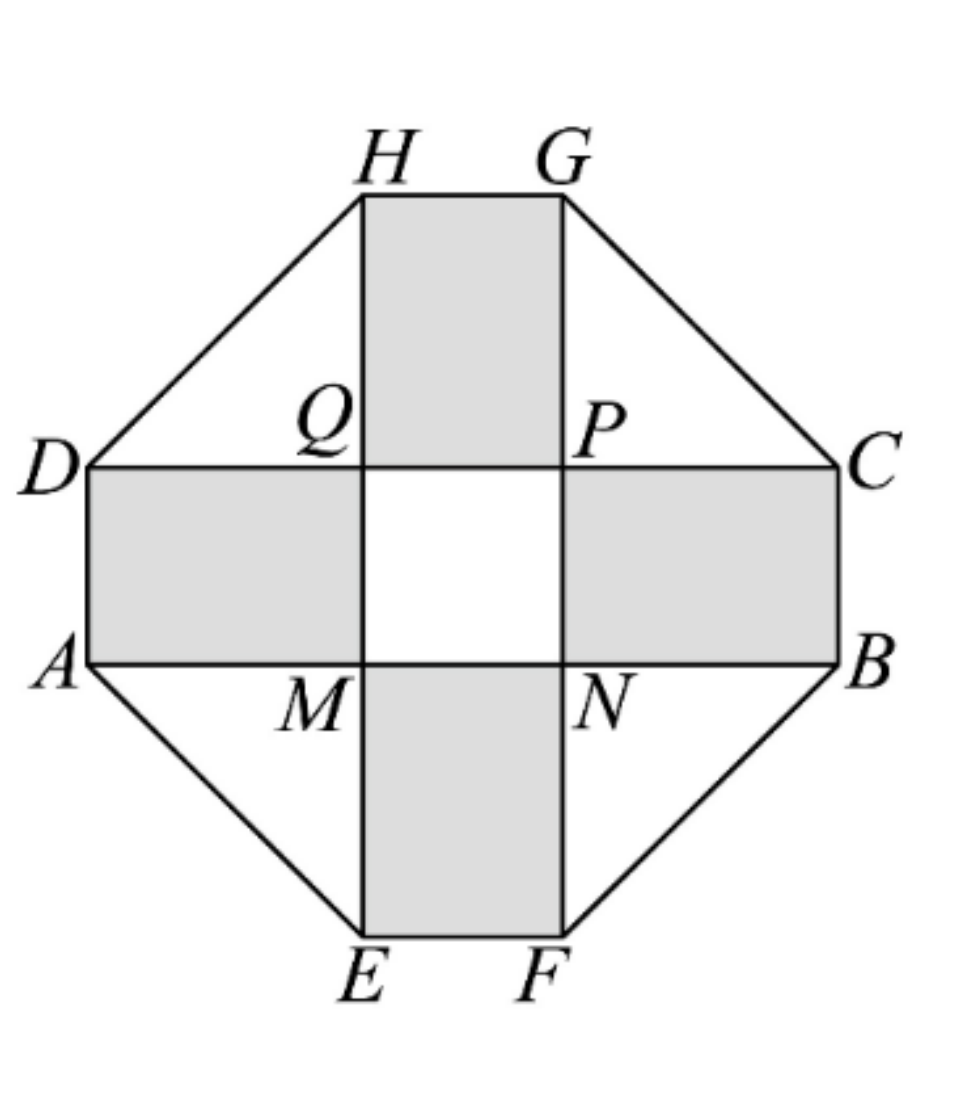
\includegraphics[width=0.34\textwidth]{figures/cross_octagon_h64.png}
\end{center}

\begin{enumerate}[label=(\arabic*)]
\item 设 $DQ$ 长为 $y\mathrm{m}$（$y>0$），用 $x$ 表示 $y$，并求出 $x$ 的取值范围；
\item 如何设计 $AD$ 可使总造价最低，并求出最低造价.
\item 若总造价 $W$ 不超过 69000 元，求 $AD$ 长 $x$ 的取值范围.
\end{enumerate}

\ifanswer
\solbegin
\stepm{(1)}{设 $DQ$ 长为 $y\mathrm{m}$，因为十字形区域面积为 $200\text{m}^2$，}
\step{所以 $4xy+x^2=200$，解得 $y=\dfrac{200-x^2}{4x}=\dfrac{50}{x}-\dfrac x4$；\dots\dots2 分}
\step{因为 $y>0$，所以 $x^2<200$，因为 $x>0$，所以 $0<x<10\sqrt2$.\dots\dots4 分}
\stepm{(2)}{四个矩形地砖面积 $S_{\text{四个矩形}}=4xy=200-x^2$，}
\step{造价 $W_{\text{四个矩形}}=105(200-x^2)$；}
\step{四个三角形草坪面积 $S_{\text{三角形}}=4\times\dfrac12y^2=2\left(\dfrac{50}{x}-\dfrac x4\right)^2=\dfrac{5000}{x^2}+\dfrac{x^2}8-50$，}
\step{造价 $W_{\text{三角形}}=40\left(\dfrac{5000}{x^2}+\dfrac{x^2}8-50\right)$；}
\step{正方形花坛面积 $S_{\text{正方形}}=x^2$，造价 $W_{\text{正方形}}=2100x^2$；}
\step{总造价 $W=W_{\text{四个矩形}}+W_{\text{三角形}}+W_{\text{正方形}}$}
\step{$=105(200-x^2)+40\left(\dfrac{5000}{x^2}+\dfrac{x^2}8-50\right)+2100x^2$，}
\step{化简得 $W=2000x^2+19000+\dfrac{200000}{x^2}$（$0<x<10\sqrt2$）.\dots\dots6 分}
\step{因为 $2000x^2+\dfrac{200000}{x^2}\geqslant40000$，}
\step{当且仅当 $x=\sqrt{10}$（在 $x$ 范围中）时取等号，此时 $W=59000$ 元.}
\step{综上，当 $AD$ 的长为 $\sqrt{10}$ 时，总造价最低，为 59000 元.\dots\dots8 分}
% 原卷 (3) 定义域印作 0<x<2√10，与 (1) 所得 0<x<10√2 不一致，照录（见文件头“原卷笔误”④）
\stepm{(3)}{由（2）得 $W=2000x^2+19000+\dfrac{200000}{x^2}$（$0<x<2\sqrt{10}$）.}
\step{总造价不超过 69000 元，即 $W=2000x^2+19000+\dfrac{200000}{x^2}\leqslant69000$，}
\step{化简得 $x^2+\dfrac{100}{x^2}\leqslant25$，\dots\dots10 分}
\step{即 $(x^2)^2-25x^2+100=(x^2-20)(x^2-5)\leqslant0$，即 $\sqrt5\leqslant x\leqslant2\sqrt5$，}
% 原卷末句“取值范围[√5,2√5]”脱“为”，照录（见文件头“原卷笔误”⑤）
\step{所以 $AD$ 长 $x$ 的取值范围$[\sqrt5,2\sqrt5]$.\dots\dots12 分}
\solend
\fi

\ansspace[10]

\item 设 $a,b,c$ 为实数，集合 $S=\{x\mid(x+a)(x^2+bx+c)=0,x\in\R\}$.

\begin{enumerate}[label=(\arabic*)]
\item 若 $a=1,b=3,c=2$，求集合 $S$；
\item 若 $S=\{-2\}$，求 $a,b,c$ 满足的条件；
\item 设 $T=\{x\mid(ax+1)(cx^2+bx+1)=0,x\in\R\}$，当 $ac\neq0$ 时，如果 $\dfrac12\in S$，$-2\in T$，且
集合 $S,T$ 均恰有两个元素，求三元数对 $(a,b,c)$.
\end{enumerate}

\ifanswer
\solbegin
\stepm{(1)}{若 $a=1,b=3,c=2$，}
\step{则方程 $(x+a)(x^2+bx+c)=0$ 为 $(x+1)(x^2+3x+2)=0$，}
\step{即 $(x+1)^2(x+2)=0$，解得 $x=-1$ 或 $x=-2$，所以 $S=\{-1,-2\}$；}
\stepm{(2)}{由题意得 $-a\in S$，因为 $S=\{-2\}$，所以 $-2$ 是方程 $x+a=0$ 的根，}
\step{即 $-2+a=0$，解得 $a=2$. 由 $S=\{-2\}$，集合 $S$ 有且仅有一个元素，}
\step{即方程 $(x+a)(x^2+bx+c)=0$ 有且仅有一个根，}
\stepm{①}{若 $-2$ 是方程 $x^2+bx+c=0$ 的根，}
\step{则 $\Delta=b^2-4c=0$，且 $-\dfrac b2=-2$，解得 $b=4,c=4$；}
\stepm{②}{若 $-2$ 不是方程 $x^2+bx+c=0$ 的根，则方程 $x^2+bx+c=0$ 无实数根，}
\step{则 $\Delta=b^2-4c<0$，}
\step{综上所述，$\begin{cases}a=2\\ b=4\\ c=4\end{cases}$ 或 $\begin{cases}a=2\\ b^2-4c<0\end{cases}$.}
\stepm{(3)}{$S=\{x\mid(x+a)(x^2+bx+c)=0,x\in\R\}$，}
\step{$T=\{x\mid(ax+1)(cx^2+bx+1)=0,x\in\R\}$，}
\step{由题意得 $a\neq0$ 且 $c\neq0$，则 $-a\in S,-\dfrac1a\in T$，}
\step{且方程 $x^2+bx+c=0$ 与 $cx^2+bx+1=0$ 有相同的判别式 $\Delta=b^2-4c$，}
\step{即两方程根的个数相同. 由集合 $S,T$ 均恰有两个元素，则 $\Delta=b^2-4c\geqslant0$.}
\step{$S=\{x\mid(x+a)(x^2+bx+c)=0,x\in\R\}$，}
\step{因为 $\dfrac12\in S$，所以 $\dfrac12$ 是方程 $x+a=0$ 或 $x^2+bx+c=0$ 的根.}
\step{$T=\{x\mid(ax+1)(cx^2+bx+1)=0,x\in\R\}$，}
\step{由 $-\dfrac1a\in T$，且 $-2\in T$，则 $-2$ 是方程 $ax+1=0$ 或 $cx^2+bx+1=0$ 的根.}
\stepm{①}{当 $a=-\dfrac12$ 时，$\dfrac12$ 是方程 $x+a=0$ 的根，$-a=\dfrac12\in S$，则 $-\dfrac1a=2\in T$，}
\step{又 $-2\in T$，则 $T=\{-2,2\}$，}
\step{由 $T=\left\{x\mid\left(-\dfrac12x+1\right)(cx^2+bx+1)=0,x\in\R\right\}$，}
% 原卷句末为句号，本稿原错作逗号
\step{则 $-2$ 是方程 $cx^2+bx+1=0$ 的根，则 $4c-2b+1=0$.}
\stepm{(i)}{若 $\Delta=b^2-4c=0$，联立 $\begin{cases}4c-2b+1=0\\ b^2-4c=0\end{cases}$ 解得 $b=1,c=\dfrac14$.}
\step{验证：当 $a=-\dfrac12,b=1,c=\dfrac14$ 时，}
\step{$S=\left\{x\mid\left(x-\dfrac12\right)\left(x^2+x+\dfrac14\right)=0,x\in\R\right\}=\left\{-\dfrac12,\dfrac12\right\}$，}
\step{$T=\left\{x\mid\left(-\dfrac12x+1\right)\left(\dfrac14x^2+x+1\right)=0,x\in\R\right\}=\{-2,2\}$，满足题意；}
\stepm{(ii)}{若 $\Delta=b^2-4c>0$，方程 $cx^2+bx+1=0$ 有两个不相等的实数根，}
\step{又 $T=\{-2,2\}$，则方程 $cx^2+bx+1=0$ 的两根必为 $-2$ 和 2.}
\step{由韦达定理得 $\begin{cases}-2+2=-\dfrac bc\\ -2\times2=\dfrac1c\end{cases}$，解得 $b=0,c=-\dfrac14$；}
\step{验证：当 $a=-\dfrac12,b=0,c=-\dfrac14$ 时，}
\step{$S=\left\{x\mid\left(x-\dfrac12\right)\left(x^2-\dfrac14\right)=0,x\in\R\right\}=\left\{-\dfrac12,\dfrac12\right\}$，}
\step{$T=\left\{x\mid\left(-\dfrac12x+1\right)\left(-\dfrac14x^2+1\right)=0,x\in\R\right\}=\{-2,2\}$，满足题意；}
\stepm{②}{当 $a=\dfrac12$ 时，$-\dfrac1a=-2$，即 $-2$ 是方程 $ax+1=0$ 的根，}
\step{则 $-a=-\dfrac12\in S$，又 $\dfrac12\in S$，则 $S=\left\{-\dfrac12,\dfrac12\right\}$，}
\step{$S=\{x\mid(x+a)(x^2+bx+c)=0,x\in\R\}$，}
\step{则 $\dfrac12$ 是方程 $x^2+bx+c=0$ 的根，则 $\dfrac14+\dfrac12b+c=0$，即 $4c+2b+1=0$；}
\stepm{(i)}{若 $\Delta=b^2-4c=0$，联立 $\begin{cases}4c+2b+1=0\\ b^2-4c=0\end{cases}$ 解得 $b=-1,c=\dfrac14$.}
\step{验证：当 $a=\dfrac12,b=-1,c=\dfrac14$ 时，}
\step{$S=\left\{x\mid\left(x+\dfrac12\right)\left(x^2-x+\dfrac14\right)=0,x\in\R\right\}=\left\{-\dfrac12,\dfrac12\right\}$，}
\step{$T=\left\{x\mid\left(\dfrac12x+1\right)\left(\dfrac14x^2-x+1\right)=0,x\in\R\right\}=\{-2,2\}$，满足题意；}
% 原卷作“有两不等的实数根”，本稿原脱“的”
\stepm{(ii)}{若 $\Delta=b^2-4c>0$，方程 $x^2+bx+c=0$ 有两不等的实数根，}
% 原卷句末为句号，本稿原错作逗号
\step{又 $S=\left\{-\dfrac12,\dfrac12\right\}$，则方程 $x^2+bx+c=0$ 的两根必为 $-\dfrac12$ 和 $\dfrac12$.}
\step{由韦达定理得 $\begin{cases}-\dfrac12+\dfrac12=-b\\ -\dfrac12\times\dfrac12=c\end{cases}$，解得 $b=0,c=-\dfrac14$；}
\step{验证：当 $a=\dfrac12,b=0,c=-\dfrac14$ 时，}
\step{$S=\left\{x\mid\left(x+\dfrac12\right)\left(x^2-\dfrac14\right)=0,x\in\R\right\}=\left\{-\dfrac12,\dfrac12\right\}$，}
\step{$T=\left\{x\mid\left(\dfrac12x+1\right)\left(-\dfrac14x^2+1\right)=0,x\in\R\right\}=\{-2,2\}$，满足题意；}
\stepm{③}{当 $a\neq-\dfrac12$ 且 $a\neq\dfrac12$ 时，则 $\dfrac12$ 不是方程 $x+a=0$ 的根，}
\step{$-2$ 也不是方程 $ax+1=0$ 的根.}
% 原卷此句单根而称“两实数根”，语病，照录（见文件头“原卷笔误”⑥）
\step{由 $\dfrac12\in S,-2\in T$，则 $\dfrac12$ 是方程 $x^2+bx+c=0$ 的两实数根，}
\step{且 $-2$ 是方程 $cx^2+bx+1=0$ 的根，则有 $\begin{cases}\dfrac14+\dfrac12b+c=0\\ 4c-2b+1=0\end{cases}$，}
\step{解得 $b=0,c=-\dfrac14$.}
\step{验证：当 $a\neq-\dfrac12$ 且 $a\neq\dfrac12,b=0,c=-\dfrac14$ 时，有 $-a\neq\dfrac12,-a\neq-\dfrac12$.}
\step{$S=\left\{x\mid(x+a)\left(x^2-\dfrac14\right)=0,x\in\R\right\}=\left\{-a,-\dfrac12,\dfrac12\right\}$ 有三个元素，}
\step{故不满足题意；}
\step{综上所述，满足题意的所有三元数对 $(a,b,c)$ 有}
\step{$\left(-\dfrac12,1,\dfrac14\right)$，$\left(-\dfrac12,0,-\dfrac14\right)$，$\left(\dfrac12,-1,\dfrac14\right)$，$\left(\dfrac12,0,-\dfrac14\right)$.}
\solend
\fi

\ansspace*[10]

\end{enumerate}

\end{document}
"
% 紧凑版：xelatex "\def\iscompact{1}% 高一64_格致中学_10月月考.tex
%   —— 高一上数学“2026-2027 年格致中学高一上 10 月月考”（讲评版）
% 试卷版：xelatex 高一64_格致中学_10月月考.tex
% 答案版：xelatex "\def\isanswer{1}% 高一64_格致中学_10月月考.tex
%   —— 高一上数学“2026-2027 年格致中学高一上 10 月月考”（讲评版）
% 试卷版：xelatex 高一64_格致中学_10月月考.tex
% 答案版：xelatex "\def\isanswer{1}\input{高一64_格致中学_10月月考.tex}"
% 紧凑版：xelatex "\def\iscompact{1}\input{高一64_格致中学_10月月考.tex}"
%
% 原始材料：微信公众号“魔都数学加油站”文章，作者破晓，连载“27学年高一64”；
% 原文标题“27学年高一64——2026-2027年上海市格致中学高一上10月月考”；
% 原文链接：https://mp.weixin.qq.com/s/0DfB77nTJf7NdVI_FYXxeA。
% 页面标注发布时间 2026-10-17 21:58（上海）。
% 本次转录只据 `原图/高一64_格致中学_10月月考/` 的 14 张 PNG 逐页读图。
% 正文为 14 张 PNG 页（`01..14.png`）：第 12、13、14 页 2560×3620，
% 第 01—11 页 4762×6735（**同一篇各页分辨率不同**），均按页序读取。
% 14 页全为试卷正文页（卷首标题在第 1 页页顶，卷末解答题第 18 题解析止于第 14 页），
% 无封面页、目录页、二维码或宣传页。粉色斜排“魔都数学加油站”为卷面水印，与公众号页脚一并未录入。
%
% 卷首标题：照卷面印作“2026--2027 年格致中学高一上 10 月月考”，年份区间按全稿惯例排 en dash。
% 原卷只有一行标题、无副标题。
%
% 篇幅与题号：原卷自第 3 题起编号（第 1、2 题不在本卷内）。填空题 3—10（8 题）、
% 选择题 11—14（4 题）、解答题 15—18（4 题），共 16 题。本稿沿用原节与原题号，
% 只改排为全稿统一的大节样式（原卷小节标题为“一、填空题”“二、选择题”“三、解答题”）。
%
% 讲评版：原卷每题下直接印【答案】或【解析】。**只印【答案】的 1 题**（第 5 题），
% 本稿只给 \ans{}；其余 15 题都印【解析】（按全稿口径这类题不另提 \ans{}——第 11、13、14 题
% 的结论写在解析末句（“故选 A”“故选 D”等），亦照录在解析内）。**另有 1 题答案印在题干括号内**——
% 第 12 题（“( B )”，该题无【答案】/【解析】段），本稿按 高一37 第 13 题成例把括号留空、
% 答案另提为 \ans{$B$}。
%
% 副标题：原卷未印副标题。本稿按“知识模块”口径标作“集合与常用逻辑用语、不等式”：
% 16 题中集合与常用逻辑用语 8 题（第 4、9、10、11、12、13、16、18 题），
% 不等式 8 题（含一元二次方程与韦达定理、基本不等式、二次不等式、恒成立、分式不等式：
% 第 3、5、6、7、8、14、15、17 题），两类均达三分之一，故并标。口径同 高一59、高一63。
%
% 与原卷的排版差异：
%   ① 原卷每题下直接印【答案】/【解析】，本稿按全稿惯例将答案与解析置于答案版，试卷版保持干净；
%   ② 原卷未印副标题，本稿按“知识模块”口径补出；
%   ③ 原卷填空横线约三四个字宽，本稿按全稿惯例统一排 \blankline[4.4em]；
%   ④ 原卷实数集排斜体 $R$（第 4、7、8、13、15、18 题）或粗体 $\mathbf{R}$（第 18 题题干与
%      解析共 6 处），整数集排斜体 $Z$（第 9、13 题）或粗体 $\mathbf{Z}$（第 9 题解析末两行），
%      有理数集排粗体 $\mathbf{Q}$（第 13 题选项 A），本稿按全稿惯例统一改用 $\R$、$\Z$、$\Q$
%      （记号归一，粗体／斜体不作区分）；空集记号原卷作 $\varnothing$，照录；
%   ⑤ 第 4 题的补集**原卷用上划线记号 $\bar B$**（题干 1 处、解析 4 处，共 5 处），
%      与全稿惯例的 $\complement_U B$ 不同，本稿照录原卷的 $\bar B$；
%   ⑥ 原卷用描述法时竖线排细竖“$|$”（如 $\{x\mid|x|\geqslant2024\}$ 一类），本稿按全稿惯例排 \mid；
%   ⑦ 第 15—18 题的子问原卷各自另起一行、以“（1）”“（2）”“（3）”标号，本稿按全稿惯例用
%      enumerate 的 (1)(2)(3)；解析中的子问标号一律用 \stepm{(1)}{…}；
%      第 18 题解析中分情形的①②③与分小目的 (i)(ii)，按全稿惯例作 \stepm{①}{…}、\stepm{(i)}{…}；
%   ⑧ 第 13 题解析的“A 选项：”“B 选项：”“C 选项：”“D 选项：”原卷排**加粗**（共 4 处），
%      同 高一63“法一：”成例，本稿排 \stepm{A 选项：}{…} 一类（加粗着色、不改黑色基调），
%      冒号照原卷排全角；
%   ⑨ 第 17 题解析带评分档，原卷在档与档之间排一串点线（“………2 分”），
%      本稿照录为“\dots\dots2 分”一类（同 高一54 成例），共 5 处；
%   ⑩ 选择题的作答括号原卷排半角“(　　)”（第 11、13、14 题括号内空白、第 12 题括号内印 B），
%      本稿按全稿惯例排 \mbox{（\quad）}；选项字母后的句点照原卷排“A.”“B.”；
%   ⑪ 每道解答题原卷未留作答空白，本稿按全稿惯例加 \ansspace（末题用 \ansspace*）；
%   ⑫ 第 17 题题干右侧的十字形八边形示意图，本稿按原卷截图裁出（`figures/cross_octagon_h64.png`，
%      原分辨率裁切，未放大、未用 TikZ 重绘），图内阴影与点名照原卷。
%
% 原卷笔误/存疑（均照录未改，正文对应处另有 % 注）：
%   ① 第 8 题解析末两步自相矛盾：上一步已化为 $\dfrac x{x-1}<0$，下一步却印作
%      “即 $x(x+1)<0$，解得 $-1<x<0$”并给出解集 $(-1,0)$——由 $\dfrac x{x-1}<0$ 应得
%      $x(x-1)<0$、解集 $(0,1)$；已 8 倍放大确认原卷确为 $x+1$ 与 $(-1,0)$，照录未改。
%   ② 第 13 题 D 选项解析“乘法满足结合率”的“率”应为“律”（同段 A、B 选项均作“结合律”）。
%   ③ 第 13 题条件①“任意 $a,b\in G$. 有 $a*b\in G$；”在 $G$ 后印句号（其余三条均以逗号
%      接下文），疑为逗号之误，照录。
%   ④ 第 17 题 (3) 解析把定义域印作 $0<x<2\sqrt{10}$，与 (1) 所得 $0<x<10\sqrt2$ 不一致
%      （疑为 $10\sqrt2$ 之误）；照录未改。
%   ⑤ 第 17 题 (3) 末句“所以 $AD$ 长 $x$ 的取值范围$[\sqrt5,2\sqrt5]$.”脱一个“为”。
%   ⑥ 第 18 题 (3) ③“则 $\dfrac12$ 是方程 $x^2+bx+c=0$ 的**两**实数根”——只有一个数却称
%      “两实数根”，语病；照录。
%
% 插图：第 17 题题干有 1 幅十字形八边形示意图（原卷第 09 页右侧），已按原卷截图排入；
% 其余 13 页无任何图形、无“如图”字样（第 17 题的“图中”均指此图）。
%
\documentclass[a4paper,11pt]{article}
\usepackage{common}

\begin{document}

\examtitlest[3]{2026--2027 年格致中学高一上 10 月月考}{集合与常用逻辑用语、不等式}

\bigsec{一、填空题}

\begin{enumerate}
\setcounter{enumi}{2}

\item 已知一元二次方程 $x^2-nx+5=0$ 的两个实根分别为 $x_1$、$x_2$，且 $\dfrac1{x_1}+\dfrac1{x_2}=1$，则实数 $n$ 的值为\blankline[4.4em].

\ifanswer
\solbegin
\step{$\dfrac1{x_1}+\dfrac1{x_2}=\dfrac{x_1+x_2}{x_1x_2}=\dfrac n5=1$，所以 $n=5$.}
\solend
\fi

\item 全集为 $U=\R$，$A=\{x\mid|x|\geqslant2\}$，$B=\{y\mid y=x^2+1,x\in\R\}$，则 $A\cup\bar B=$\blankline[4.4em].

\ifanswer
\solbegin
\step{由题意得集合 $A=\{x\mid x\geqslant2\text{ 或 }x\leqslant-2\}$，}
\step{因为 $x^2+1\geqslant1$，所以集合 $B=\{x\mid x\geqslant1\}$，所以 $\bar B=\{x\mid x<1\}$，}
\step{则 $A\cup\bar B=\{x\mid x\geqslant2\text{ 或 }x<1\}$.}
\solend
\fi

\item 若 $x>2$，则 $4x+\dfrac1{x-2}$ 的最小值为\blankline[4.4em].

\ifanswer
\ans{$12$}
\fi

\item 已知关于 $x$ 不等式组$\begin{cases}(3x-2)(2x+3)\leqslant0\\ x-a<0\end{cases}$\!没有实数解，则实数 $a$ 的取值范围为\blankline[4.4em].

\ifanswer
\solbegin
\step{由题意得 $\begin{cases}-\dfrac32\leqslant x\leqslant\dfrac23\\ x<a\end{cases}$ 无解，所以 $a\leqslant-\dfrac32$.}
\solend
\fi

\item 若不等式 $\dfrac{x^2-8x+20}{mx^2-mx-1}<0$ 对一切 $x\in\R$ 都成立，则实数 $m$ 的取值范围为\blankline[4.4em].

\ifanswer
\solbegin
\step{因为 $x^2-8x+20=(x-4)^2+4\geqslant4>0$，所以 $mx^2-mx-1<0$，}
\step{当 $m=0$ 时，$mx^2-mx-1=-1<0$，不等式成立；}
\step{设 $y=mx^2-mx-1$，当 $m\neq0$ 时函数 $y$ 为二次函数，$y$ 要恒小于 0，}
\step{抛物线开口向下且与 $x$ 轴没有交点，即 $m<0$ 且 $\Delta<0$，得 $-4<m\leqslant0$，}
\step{故实数 $m$ 的取值范围为 $(-4,0]$.}
\solend
\fi

\item 已知关于 $x$ 的不等式 $\dfrac{ax-1}{x+b}>0$ 的解集为 $\{x\mid-1<x<2\}$，其中 $a$、$b\in\R$，则关于 $x$ 的不等式 $\dfrac{bx+1}{ax+1}<1$ 的解集为\blankline[4.4em].

\ifanswer
\solbegin
\step{不等式 $\dfrac{ax-1}{x+b}>0$ 等价于 $(ax-1)(x+b)>0$，即 $ax^2+(ab-1)x-b>0$，}
\step{所以 $-1$ 和 2 为方程 $ax^2+(ab-1)x-b=0$ 的两根，且 $a<0$，}
\step{由韦达定理得 $\begin{cases}-1+2=-\dfrac{ab-1}a\\ -1\times2=-\dfrac ba\end{cases}$，解得 $\begin{cases}a=-1\\ b=-2\end{cases}$，}
\step{所以原不等式为 $\dfrac{-2x+1}{-x+1}<1\Rightarrow\dfrac{-2x+1}{-x+1}-1<0\Rightarrow\dfrac{-x}{-x+1}<0\Rightarrow\dfrac x{x-1}<0$，}
% 原卷下一步印作“即 x(x+1)<0，解得 -1<x<0”，与上一步 x/(x-1)<0 不等价，
% 照录未改（见文件头“原卷笔误”①）
\step{即 $x(x+1)<0$，解得 $-1<x<0$，即不等式 $\dfrac{bx+1}{ax+1}<1$ 的解集为 $(-1,0)$.}
\solend
\fi

\item 已知集合 $M=\{x\mid|x|\leqslant2024,x\in\Z\}$，集合 $P$ 是 $M$ 的三元子集，即 $P=\{a,b,c\}\subseteq M$，$P$~中元素 $a,b,c$ 满足 $\begin{cases}\dfrac1a+\dfrac1b=\dfrac2c\\ a+c=2b\end{cases}$，则符合要求的集合 $P$ 有\blankline[4.4em]个.

\ifanswer
\solbegin
\step{由 $a+c=2b$，则 $a=2b-c$，代入 $\dfrac1a+\dfrac1b=\dfrac2c$，即 $\dfrac1{2b-c}=\dfrac2c-\dfrac1b=\dfrac{2b-c}{bc}$，}
\step{整理得 $(2b-c)^2=bc$，展开得 $4b^2-5bc+c^2=0$，}
\step{解得 $b=\dfrac c4$ 或 $b=c$（由集合的互异性，舍去），代入 $a+c=2b$ 得 $a=-\dfrac c2$，}
\step{则 $P=\left\{-\dfrac c2,\dfrac c4,c\right\}\subseteq\{x\mid-2024\leqslant x\leqslant2024,x\in\Z\}$，所以 $c$ 为 4 的整数倍，}
\step{且不为 0，则共有 $\dfrac{2024}4\times2=1012$ 个.}
\solend
\fi

\item 已知正整数 $n\geqslant2$，对集合 $\{1,2,3,\cdots,n\}$ 及其每一个非空子集 $X$，记
$X=\{x_1,x_2,\cdots,x_k\}$，其中 $x_1>x_2>\cdots>x_k$，定义一个运算“交替和”
$S_X=x_1-x_2+x_3\cdots+(-1)^{k+1}x_k$. 例如：对于集合 $X=\{9,6,4,2,1\}$，
$S_X=9-6+4-2+1=6$. 则当 $n=7$ 时，集合 $\{1,2,3,\cdots,n\}$ 的所有子集的“交替和”的总
和为\blankline[4.4em].

\ifanswer
\solbegin
\step{由题意得集合 $\{7\}$ 的“交替和”为 7.}
\step{集合 $\{1,2,3,4,5,6,7\}$ 的所有 $2^7$ 个子集中，除去集合 $\{7\}$ 外，}
\step{还有 $2^7-2$ 个非空子集，这 $2^7-2$ 个非空子集中不含元素 7 的集合，}
\step{即 $\{1,2,3,4,5,6\}$ 的非空子集，共有 $2^6-1$ 个，设为 $A_i(i=1,2,\cdots,2^6-1)$；}
\step{则这 $2^7-2$ 个非空子集中含元素 7 的集合，也共有 $2^6-1$ 个，}
\step{这样的集合都可以看成相应地在每个不含 7 的集合中再加上元素 7 得到，}
\step{即 $A_i\cup\{7\}$.}
\step{对 $A_i(i=1,2,\cdots,2^6-1)$ 中的任意集合 $A$，记 $A=\{x_1,x_2,\cdots,x_k\}$，}
\step{则“交替和”$S_A=x_1-x_2+x_3\cdots+(-1)^{k+1}x_k$，其中 $x_1>x_2>\cdots>x_k$，}
\step{由 $7>x_1>x_2>\cdots>x_k$，}
\step{则集合 $A\cup\{7\}$ 的“交替和”为 $7-[x_1-x_2+x_3\cdots+(-1)^{k+1}x_k]$，}
\step{则集合 $A$ 与集合 $A\cup\{7\}$ 的“交替和”之和为 7，下面举例说明：}
\step{如集合 $\{6,5,4,3,2,1\}$ 与集合 $\{7,6,5,4,3,2,1\}$，}
\step{$\{6,5,4,3,2,1\}$ 的“交替和”为 $6-5+4-3+2-1=3$，}
% 原卷此句在页末折为两个印刷行（“……的“交替和”为”／“7-6+5-4+3-2+1=……”），
% 本稿原并作一条，现照原卷拆开（原卷原样两行 / 本稿原错处：并作一行）
\step{$\{7,6,5,4,3,2,1\}$ 的“交替和”为}
\step{$7-6+5-4+3-2+1=7-(6-5+4-3+2-1)=7-3$，}
\step{即集合 $\{6,5,4,3,2,1\}$ 与集合 $\{7,6,5,4,3,2,1\}$ 的“交替和”之和为 7.}
\step{综上，把这 $2^7-2$ 个非空子集两两结组后分别计算每一组中“交替和”之和，}
\step{且每组中“交替和”之和都为 7，共有 $2^6-1$ 组.}
\step{故集合 $\{1,2,3,4,5,6,7\}$ 所有“交替和”之和，}
\step{由各组之和再加集合 $\{7\}$ 的“交替和”7 即可，}
\step{综上所述，当 $n=7$ 时，集合 $\{1,2,3,\cdots,n\}$ 的所有子集的所有“交替和”之和}
\step{为 $7\times(2^6-1)+7=448$.}
\solend
\fi

\end{enumerate}

\bigsec{二、选择题}

\begin{enumerate}
\setcounter{enumi}{10}

\item 若 $a$、$b\in\R$，则“$a<b<0$”是“$a^2>b^2$”的\mbox{（\quad）}条件.

\keepwithprev
A. 充分非必要\qquad B. 必要非充分

C. 充要\qquad D. 既非充分也非必要

\ifanswer
\solbegin
\step{由 $a<b<0\Rightarrow-a>-b>0\Rightarrow(-a)^2>(-b)^2\Rightarrow a^2>b^2$，}
\step{因此由 $a<b<0$ 可以推出 $a^2>b^2$，}
\step{但是当 $a=1$，$b=0$ 时，显然 $a^2>b^2$ 成立，但是 $a<b<0$ 不成立，}
\step{因此由 $a^2>b^2$ 不一定能推出 $a<b<0$，}
\step{因此“$a<b<0$”是“$a^2>b^2$”的充分非必要条件. 故选 $A$.}
\solend
\fi

% 第 12 题答案“B”直接印在题干括号内“(  B  )”，且该题无【答案】/【解析】段；
% 按 高一37 第 13 题的成例括号留空、答案另提为 \ans{}（见文件头）
\item 用反证法证明结论“$a$、$b$、$c$ 至少有一个是正数”时，应假设\mbox{（\quad）}

\keepwithprev
A. $a$、$b$、$c$ 都是正数\qquad B. $a$、$b$、$c$ 都不是正数

C. $a$、$b$、$c$ 至多有一个正数\qquad D. $a$、$b$、$c$ 至多有两个正数

\ifanswer
\ans{$B$}
\fi

\item “群”的概念由数学家伽罗瓦在 19 世纪 30 年代开创，群论虽起源于对代数多项式方程
的研究，但在量子力学、晶体结构学等其他学科中也有十分广泛的应用.“群”的定义是：

设 $G$ 为某种元素组成的一个非空集合，若在 $G$ 内定义一个运算“*”，满足以下条件：

% 原卷条件①在 G 后印句号，疑为逗号之误，照录（见文件头“原卷笔误”③）
①任意 $a,b\in G$. 有 $a*b\in G$；

②如 $a,b,c\in G$，有 $(a*b)*c=a*(b*c)$；

③在 $G$ 中有一个元素 $e$，对任意 $a\in G$，都有 $a*e=e*a=a$，称 $e$ 为 $G$ 的单位元；

④任意 $a\in G$，在 $G$ 中存在唯一确定的 $b$，使 $a*b=b*a=e$，称 $b$ 为 $a$ 的逆元；

此时称 $(G,*)$ 为一个群.

例如实数集 $\R$ 和实数集上的加法运算“+”就构成一个群 $(\R,+)$，其单位元是 0，每一个数
的逆元是其相反数，那么下列说法中，错误的是\mbox{（\quad）}

\keepwithprev
A. $G=\Q$，则 $(G,+)$ 为一个群

B. $G=\{\sqrt2m+\sqrt3n\mid m,n\in\Z\}$，$(G,+)$ 为一个群

C. $G=\{-1,1\}$，则 $(G,\times)$ 为一个群

D. $G=\{x\mid x=2k+1,k\in\Z\}$，则 $(G,\times)$ 为一个群

\ifanswer
\solbegin
\stepm{A 选项：}{有理数的和还是有理数，求和满足结合律，}
\step{设 $a\in\Q$，单位元为 $e$，则 $a+e=a$，故 $e=0$，}
\step{所以每一个数的相反数为其逆元，故 $(G,+)$ 为一个群，选项 A 正确；}
\stepm{B 选项：}{$G=\{\sqrt2m+\sqrt3n\mid m,n\in\Z\}$ 中的任何两个数相加还是属于}
\step{$G=\{\sqrt2m+\sqrt3n\mid m,n\in\Z\}$，求和满足结合律，}
\step{设 $\sqrt2x+\sqrt3y\in G,x,y\in\Z$，单位元为 $e$，}
\step{则 $\sqrt2x+\sqrt3y+e=\sqrt2x+\sqrt3y$，所以 $e=0$，}
\step{每一个数的相反数为其逆元，$(G,+)$ 为一个群，选项 B 正确；}
\stepm{C 选项：}{$G=\{-1,1\}$ 中的两个元素相乘，其积可能为 1 或 $-1$，又 $1\in G,-1\in G$，}
\step{设 $a\in G$，单位元为 $e$，则 $a\times e=a$，故 $e=1,1$ 的逆元为 $1,-1$ 的逆元为 $-1$，}
\step{所以 $(G,\times)$ 为一个群，选项 C 正确；}
% 原卷“乘法满足结合率”的“率”应为“律”（同段 A、B 选项均作“结合律”），照录（见文件头“原卷笔误”②）
\stepm{D 选项：}{两个奇数相乘还是奇数，乘法满足结合率，}
\step{设 $a\in G$，单位元为 $e$，则 $a\times e=a$，故 $e=1$，}
\step{又 $3\in G$，故存在 $b\in G$，使得 $3b=1$，则 $b=\dfrac13$，矛盾，}
\step{故 $(G,\times)$ 不为一个群，选项 D 错误.}
\step{故选 $D$.}
\solend
\fi

\item 已知 $a$、$b$、$c\in\R$，若关于 $x$ 的不等式 $0\leqslant x+\dfrac ax+b\leqslant\dfrac cx-1$ 的解集为 $[x_1,x_2]\cup\{x_3\}$
（$x_3>x_2>x_1>0$），则\mbox{（\quad）}

\keepwithprev
A. 不存在有序数组 $(a,b,c)$，使得 $x_2-x_1=1$

B. 存在唯一有序数组 $(a,b,c)$，使得 $x_2-x_1=1$

C. 有且只有两组有序数组 $(a,b,c)$，使得 $x_2-x_1=1$

D. 存在无穷多组有序数组 $(a,b,c)$，使得 $x_2-x_1=1$

\ifanswer
\solbegin
\step{因为不等式 $0\leqslant x+\dfrac ax+b\leqslant\dfrac cx-1$ 的解集为 $[x_1,x_2]\cup\{x_3\}$（$x_3>x_2>x_1>0$），}
\step{所以 $0\leqslant x^2+bx+a\leqslant c-x$ 在 $[x_1,x_2]\cup\{x_3\}$ 上成立，}
\step{假设 $x_1=m$，$x_2=m+1$，$x_3=n$，}
\step{则 $c-n=0=n^2+bn+a$，由 $x_3$ 为一个独立的数得出，}
\step{所以 $n=c$，且 $m+1$ 与 $n$ 为方程 $x^2+bx+a=0$ 的两个根，}
\step{因为 $x_3>x_2>x_1>0$，所以 $-b=m+n+1=m+c+1$，$a=mn+n=mc+c$，}
\step{所以 $b=-m-c-1$，}
\step{且点 $(x_1,x_1^2+bx_1+a)$ 为 $y=x^2+bx+a$ 与 $y=c-x$ 的左交点，}
\step{所以 $m^2+bm+a=c-m$ 且 $b=-m-c-1$，$a=mc+c$，}
\step{故 $m^2+bm+a=m^2-m^2-mc-m+mc+c=c-m$，所以 $c-m=c-m$ 恒成立，}
\step{所以不论 $a$、$b$、$c$ 取何值，$x_2-x_1=1$ 恒成立，}
\step{即存在无穷多组有序数组 $(a,b,c)$，使得 $x_2-x_1=1$，}
\step{故选项 $A$、$B$、$C$ 错误，选项 $D$ 正确. 故选 $D$.}
\solend
\fi

\end{enumerate}

\bigsec{三、解答题}

\begin{enumerate}
\setcounter{enumi}{14}

\item 已知函数 $f(x)=(a-1)x^2-ax+1$，$a\in\R$.

\begin{enumerate}[label=(\arabic*)]
\item 若不等式 $f(x)<0$ 的解集为 $\left(\dfrac13,1\right)$，求实数 $a$ 的值；
\item 当 $a>1$ 时，解关于 $x$ 的不等式 $f(x)\geqslant0$.
\end{enumerate}

\ifanswer
\solbegin
\stepm{(1)}{因为不等式 $f(x)<0$ 的解集为 $\left(\dfrac13,1\right)$，}
\step{所以不等式对应的方程 $(a-1)x^2-ax+1=0$ 的两根分别为 $\dfrac13$、1，}
\step{由根与系数的关系得 $\begin{cases}1+\dfrac13=\dfrac a{a-1}\\ 1\times\dfrac13=\dfrac1{a-1}\end{cases}$，解得 $a=4$；}
\stepm{(2)}{不等式 $(a-1)x^2-ax+1\geqslant0$（$a>1$）可化为 $(x-1)[(a-1)x-1]\geqslant0$，}
\step{不等式对应方程的两根为 $x_1=1$，$x_2=\dfrac1{a-1}$，}
\step{①当 $\dfrac1{a-1}=1$，即 $a=2$ 时，不等式为 $(x-1)^2\geqslant0$，解集为 $\R$；}
\step{②当 $\dfrac1{a-1}>1$，即 $1<a<2$ 时，解不等式得 $x\leqslant1$ 或 $x\geqslant\dfrac1{a-1}$；}
\step{③当 $\dfrac1{a-1}<1$，即 $a>2$ 时，解不等式得 $x\leqslant\dfrac1{a-1}$ 或 $x\geqslant1$；}
\step{综上，$a=2$ 时，不等式的解集为 $\R$，}
\step{$1<a<2$ 时，不等式的解集为 $(-\infty,1]\cup\left[\dfrac1{a-1},+\infty\right)$，}
\step{$a>2$ 时，不等式的解集为 $\left(-\infty,\dfrac1{a-1}\right]\cup[1,+\infty)$.}
\solend
\fi

\ansspace[6]

\item 若集合 $A=\{x\mid x^2+5x-6=0\}$，$B=\{x\mid x^2+2(m+1)x+m^2-3=0\}$.

\begin{enumerate}[label=(\arabic*)]
\item 若 $m=0$，写出 $A\cup B$ 的子集个数；
\item 若 $A\cap B=B$，求实数 $m$ 的取值范围.
\end{enumerate}

\ifanswer
\solbegin
\stepm{(1)}{当 $m=0$ 时，$B=\{1,-3\}$，}
\step{因为 $A=\{x\mid x^2+5x-6=0\}=\{-6,1\}$，}
\step{所以 $A\cup B=\{-6,-3,1\}$，集合元素个数为 3 个，}
\step{故 $A\cup B$ 的子集个数为 $2^3=8$.}
\stepm{(2)}{因为 $A\cap B=B$，所以 $B\subseteq A$，}
\step{$\Delta=4(m+1)^2-4(m^2-3)=8m+16$，}
\step{当 $\Delta<0$，即 $m<-2$ 时，$B=\varnothing$，符合题意，}
\step{当 $\Delta=0$，即 $m=-2$ 时，$B=\{1\}$，符合题意，}
\step{当 $\Delta>0$，即 $m>-2$ 时，若 $B\subseteq A$，则 $B=\{-6,1\}$，}
\step{即 $\begin{cases}-2(m+1)=-5\\ m^2-3=-6\end{cases}$，方程组无解，}
\step{综上所述，$m$ 的取值范围为 $(-\infty,-2]$.}
\solend
\fi

\ansspace[6]

\item 2025 年上海奇迹花园国际艺术花展于 9 月 20 日正式启幕，本次花展首次实现沉浸 IP
展、花卉景观、跨界艺术、光影夜花园四展合一，为市民游客打造一个可游、可赏、可感
的秋季治愈系童话世界. 某公园受此启发打算设计一个八边形活动区域，该区域的主体造
型平面图是由两个相同的矩形 $ABCD$ 和 $EFGH$ 构成的十字形地域，十字形的面积为
$200\text{m}^2$. 计划在正方形 $MNPQ$ 上建一座花坛，造价为 2100 元$/\text{m}^2$；在四个相同的矩形
（图中阴影部分）上铺地砖，造价为 105 元$/\text{m}^2$；再在四个空角（图中四个三角
形）上铺草坪，造价为 40 元$/\text{m}^2$. 设 $AD$ 长为 $x\mathrm{m}$（$x>0$），总造价为 $W$ 元，求：

\begin{center}
% 插图取自原卷第 09 页右侧截图（原分辨率裁切，未用 TikZ 重绘），阴影与点名照原卷
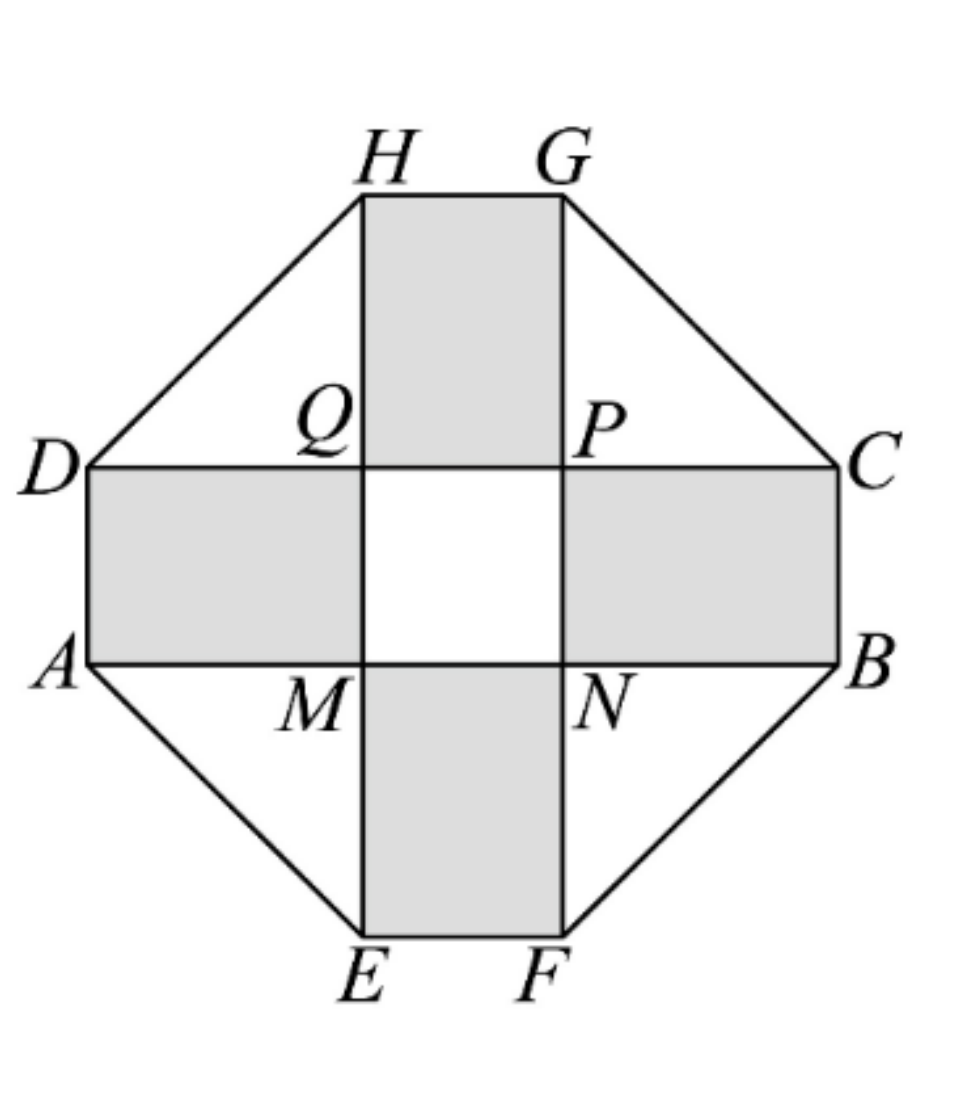
\includegraphics[width=0.34\textwidth]{figures/cross_octagon_h64.png}
\end{center}

\begin{enumerate}[label=(\arabic*)]
\item 设 $DQ$ 长为 $y\mathrm{m}$（$y>0$），用 $x$ 表示 $y$，并求出 $x$ 的取值范围；
\item 如何设计 $AD$ 可使总造价最低，并求出最低造价.
\item 若总造价 $W$ 不超过 69000 元，求 $AD$ 长 $x$ 的取值范围.
\end{enumerate}

\ifanswer
\solbegin
\stepm{(1)}{设 $DQ$ 长为 $y\mathrm{m}$，因为十字形区域面积为 $200\text{m}^2$，}
\step{所以 $4xy+x^2=200$，解得 $y=\dfrac{200-x^2}{4x}=\dfrac{50}{x}-\dfrac x4$；\dots\dots2 分}
\step{因为 $y>0$，所以 $x^2<200$，因为 $x>0$，所以 $0<x<10\sqrt2$.\dots\dots4 分}
\stepm{(2)}{四个矩形地砖面积 $S_{\text{四个矩形}}=4xy=200-x^2$，}
\step{造价 $W_{\text{四个矩形}}=105(200-x^2)$；}
\step{四个三角形草坪面积 $S_{\text{三角形}}=4\times\dfrac12y^2=2\left(\dfrac{50}{x}-\dfrac x4\right)^2=\dfrac{5000}{x^2}+\dfrac{x^2}8-50$，}
\step{造价 $W_{\text{三角形}}=40\left(\dfrac{5000}{x^2}+\dfrac{x^2}8-50\right)$；}
\step{正方形花坛面积 $S_{\text{正方形}}=x^2$，造价 $W_{\text{正方形}}=2100x^2$；}
\step{总造价 $W=W_{\text{四个矩形}}+W_{\text{三角形}}+W_{\text{正方形}}$}
\step{$=105(200-x^2)+40\left(\dfrac{5000}{x^2}+\dfrac{x^2}8-50\right)+2100x^2$，}
\step{化简得 $W=2000x^2+19000+\dfrac{200000}{x^2}$（$0<x<10\sqrt2$）.\dots\dots6 分}
\step{因为 $2000x^2+\dfrac{200000}{x^2}\geqslant40000$，}
\step{当且仅当 $x=\sqrt{10}$（在 $x$ 范围中）时取等号，此时 $W=59000$ 元.}
\step{综上，当 $AD$ 的长为 $\sqrt{10}$ 时，总造价最低，为 59000 元.\dots\dots8 分}
% 原卷 (3) 定义域印作 0<x<2√10，与 (1) 所得 0<x<10√2 不一致，照录（见文件头“原卷笔误”④）
\stepm{(3)}{由（2）得 $W=2000x^2+19000+\dfrac{200000}{x^2}$（$0<x<2\sqrt{10}$）.}
\step{总造价不超过 69000 元，即 $W=2000x^2+19000+\dfrac{200000}{x^2}\leqslant69000$，}
\step{化简得 $x^2+\dfrac{100}{x^2}\leqslant25$，\dots\dots10 分}
\step{即 $(x^2)^2-25x^2+100=(x^2-20)(x^2-5)\leqslant0$，即 $\sqrt5\leqslant x\leqslant2\sqrt5$，}
% 原卷末句“取值范围[√5,2√5]”脱“为”，照录（见文件头“原卷笔误”⑤）
\step{所以 $AD$ 长 $x$ 的取值范围$[\sqrt5,2\sqrt5]$.\dots\dots12 分}
\solend
\fi

\ansspace[10]

\item 设 $a,b,c$ 为实数，集合 $S=\{x\mid(x+a)(x^2+bx+c)=0,x\in\R\}$.

\begin{enumerate}[label=(\arabic*)]
\item 若 $a=1,b=3,c=2$，求集合 $S$；
\item 若 $S=\{-2\}$，求 $a,b,c$ 满足的条件；
\item 设 $T=\{x\mid(ax+1)(cx^2+bx+1)=0,x\in\R\}$，当 $ac\neq0$ 时，如果 $\dfrac12\in S$，$-2\in T$，且
集合 $S,T$ 均恰有两个元素，求三元数对 $(a,b,c)$.
\end{enumerate}

\ifanswer
\solbegin
\stepm{(1)}{若 $a=1,b=3,c=2$，}
\step{则方程 $(x+a)(x^2+bx+c)=0$ 为 $(x+1)(x^2+3x+2)=0$，}
\step{即 $(x+1)^2(x+2)=0$，解得 $x=-1$ 或 $x=-2$，所以 $S=\{-1,-2\}$；}
\stepm{(2)}{由题意得 $-a\in S$，因为 $S=\{-2\}$，所以 $-2$ 是方程 $x+a=0$ 的根，}
\step{即 $-2+a=0$，解得 $a=2$. 由 $S=\{-2\}$，集合 $S$ 有且仅有一个元素，}
\step{即方程 $(x+a)(x^2+bx+c)=0$ 有且仅有一个根，}
\stepm{①}{若 $-2$ 是方程 $x^2+bx+c=0$ 的根，}
\step{则 $\Delta=b^2-4c=0$，且 $-\dfrac b2=-2$，解得 $b=4,c=4$；}
\stepm{②}{若 $-2$ 不是方程 $x^2+bx+c=0$ 的根，则方程 $x^2+bx+c=0$ 无实数根，}
\step{则 $\Delta=b^2-4c<0$，}
\step{综上所述，$\begin{cases}a=2\\ b=4\\ c=4\end{cases}$ 或 $\begin{cases}a=2\\ b^2-4c<0\end{cases}$.}
\stepm{(3)}{$S=\{x\mid(x+a)(x^2+bx+c)=0,x\in\R\}$，}
\step{$T=\{x\mid(ax+1)(cx^2+bx+1)=0,x\in\R\}$，}
\step{由题意得 $a\neq0$ 且 $c\neq0$，则 $-a\in S,-\dfrac1a\in T$，}
\step{且方程 $x^2+bx+c=0$ 与 $cx^2+bx+1=0$ 有相同的判别式 $\Delta=b^2-4c$，}
\step{即两方程根的个数相同. 由集合 $S,T$ 均恰有两个元素，则 $\Delta=b^2-4c\geqslant0$.}
\step{$S=\{x\mid(x+a)(x^2+bx+c)=0,x\in\R\}$，}
\step{因为 $\dfrac12\in S$，所以 $\dfrac12$ 是方程 $x+a=0$ 或 $x^2+bx+c=0$ 的根.}
\step{$T=\{x\mid(ax+1)(cx^2+bx+1)=0,x\in\R\}$，}
\step{由 $-\dfrac1a\in T$，且 $-2\in T$，则 $-2$ 是方程 $ax+1=0$ 或 $cx^2+bx+1=0$ 的根.}
\stepm{①}{当 $a=-\dfrac12$ 时，$\dfrac12$ 是方程 $x+a=0$ 的根，$-a=\dfrac12\in S$，则 $-\dfrac1a=2\in T$，}
\step{又 $-2\in T$，则 $T=\{-2,2\}$，}
\step{由 $T=\left\{x\mid\left(-\dfrac12x+1\right)(cx^2+bx+1)=0,x\in\R\right\}$，}
% 原卷句末为句号，本稿原错作逗号
\step{则 $-2$ 是方程 $cx^2+bx+1=0$ 的根，则 $4c-2b+1=0$.}
\stepm{(i)}{若 $\Delta=b^2-4c=0$，联立 $\begin{cases}4c-2b+1=0\\ b^2-4c=0\end{cases}$ 解得 $b=1,c=\dfrac14$.}
\step{验证：当 $a=-\dfrac12,b=1,c=\dfrac14$ 时，}
\step{$S=\left\{x\mid\left(x-\dfrac12\right)\left(x^2+x+\dfrac14\right)=0,x\in\R\right\}=\left\{-\dfrac12,\dfrac12\right\}$，}
\step{$T=\left\{x\mid\left(-\dfrac12x+1\right)\left(\dfrac14x^2+x+1\right)=0,x\in\R\right\}=\{-2,2\}$，满足题意；}
\stepm{(ii)}{若 $\Delta=b^2-4c>0$，方程 $cx^2+bx+1=0$ 有两个不相等的实数根，}
\step{又 $T=\{-2,2\}$，则方程 $cx^2+bx+1=0$ 的两根必为 $-2$ 和 2.}
\step{由韦达定理得 $\begin{cases}-2+2=-\dfrac bc\\ -2\times2=\dfrac1c\end{cases}$，解得 $b=0,c=-\dfrac14$；}
\step{验证：当 $a=-\dfrac12,b=0,c=-\dfrac14$ 时，}
\step{$S=\left\{x\mid\left(x-\dfrac12\right)\left(x^2-\dfrac14\right)=0,x\in\R\right\}=\left\{-\dfrac12,\dfrac12\right\}$，}
\step{$T=\left\{x\mid\left(-\dfrac12x+1\right)\left(-\dfrac14x^2+1\right)=0,x\in\R\right\}=\{-2,2\}$，满足题意；}
\stepm{②}{当 $a=\dfrac12$ 时，$-\dfrac1a=-2$，即 $-2$ 是方程 $ax+1=0$ 的根，}
\step{则 $-a=-\dfrac12\in S$，又 $\dfrac12\in S$，则 $S=\left\{-\dfrac12,\dfrac12\right\}$，}
\step{$S=\{x\mid(x+a)(x^2+bx+c)=0,x\in\R\}$，}
\step{则 $\dfrac12$ 是方程 $x^2+bx+c=0$ 的根，则 $\dfrac14+\dfrac12b+c=0$，即 $4c+2b+1=0$；}
\stepm{(i)}{若 $\Delta=b^2-4c=0$，联立 $\begin{cases}4c+2b+1=0\\ b^2-4c=0\end{cases}$ 解得 $b=-1,c=\dfrac14$.}
\step{验证：当 $a=\dfrac12,b=-1,c=\dfrac14$ 时，}
\step{$S=\left\{x\mid\left(x+\dfrac12\right)\left(x^2-x+\dfrac14\right)=0,x\in\R\right\}=\left\{-\dfrac12,\dfrac12\right\}$，}
\step{$T=\left\{x\mid\left(\dfrac12x+1\right)\left(\dfrac14x^2-x+1\right)=0,x\in\R\right\}=\{-2,2\}$，满足题意；}
% 原卷作“有两不等的实数根”，本稿原脱“的”
\stepm{(ii)}{若 $\Delta=b^2-4c>0$，方程 $x^2+bx+c=0$ 有两不等的实数根，}
% 原卷句末为句号，本稿原错作逗号
\step{又 $S=\left\{-\dfrac12,\dfrac12\right\}$，则方程 $x^2+bx+c=0$ 的两根必为 $-\dfrac12$ 和 $\dfrac12$.}
\step{由韦达定理得 $\begin{cases}-\dfrac12+\dfrac12=-b\\ -\dfrac12\times\dfrac12=c\end{cases}$，解得 $b=0,c=-\dfrac14$；}
\step{验证：当 $a=\dfrac12,b=0,c=-\dfrac14$ 时，}
\step{$S=\left\{x\mid\left(x+\dfrac12\right)\left(x^2-\dfrac14\right)=0,x\in\R\right\}=\left\{-\dfrac12,\dfrac12\right\}$，}
\step{$T=\left\{x\mid\left(\dfrac12x+1\right)\left(-\dfrac14x^2+1\right)=0,x\in\R\right\}=\{-2,2\}$，满足题意；}
\stepm{③}{当 $a\neq-\dfrac12$ 且 $a\neq\dfrac12$ 时，则 $\dfrac12$ 不是方程 $x+a=0$ 的根，}
\step{$-2$ 也不是方程 $ax+1=0$ 的根.}
% 原卷此句单根而称“两实数根”，语病，照录（见文件头“原卷笔误”⑥）
\step{由 $\dfrac12\in S,-2\in T$，则 $\dfrac12$ 是方程 $x^2+bx+c=0$ 的两实数根，}
\step{且 $-2$ 是方程 $cx^2+bx+1=0$ 的根，则有 $\begin{cases}\dfrac14+\dfrac12b+c=0\\ 4c-2b+1=0\end{cases}$，}
\step{解得 $b=0,c=-\dfrac14$.}
\step{验证：当 $a\neq-\dfrac12$ 且 $a\neq\dfrac12,b=0,c=-\dfrac14$ 时，有 $-a\neq\dfrac12,-a\neq-\dfrac12$.}
\step{$S=\left\{x\mid(x+a)\left(x^2-\dfrac14\right)=0,x\in\R\right\}=\left\{-a,-\dfrac12,\dfrac12\right\}$ 有三个元素，}
\step{故不满足题意；}
\step{综上所述，满足题意的所有三元数对 $(a,b,c)$ 有}
\step{$\left(-\dfrac12,1,\dfrac14\right)$，$\left(-\dfrac12,0,-\dfrac14\right)$，$\left(\dfrac12,-1,\dfrac14\right)$，$\left(\dfrac12,0,-\dfrac14\right)$.}
\solend
\fi

\ansspace*[10]

\end{enumerate}

\end{document}
"
% 紧凑版：xelatex "\def\iscompact{1}% 高一64_格致中学_10月月考.tex
%   —— 高一上数学“2026-2027 年格致中学高一上 10 月月考”（讲评版）
% 试卷版：xelatex 高一64_格致中学_10月月考.tex
% 答案版：xelatex "\def\isanswer{1}\input{高一64_格致中学_10月月考.tex}"
% 紧凑版：xelatex "\def\iscompact{1}\input{高一64_格致中学_10月月考.tex}"
%
% 原始材料：微信公众号“魔都数学加油站”文章，作者破晓，连载“27学年高一64”；
% 原文标题“27学年高一64——2026-2027年上海市格致中学高一上10月月考”；
% 原文链接：https://mp.weixin.qq.com/s/0DfB77nTJf7NdVI_FYXxeA。
% 页面标注发布时间 2026-10-17 21:58（上海）。
% 本次转录只据 `原图/高一64_格致中学_10月月考/` 的 14 张 PNG 逐页读图。
% 正文为 14 张 PNG 页（`01..14.png`）：第 12、13、14 页 2560×3620，
% 第 01—11 页 4762×6735（**同一篇各页分辨率不同**），均按页序读取。
% 14 页全为试卷正文页（卷首标题在第 1 页页顶，卷末解答题第 18 题解析止于第 14 页），
% 无封面页、目录页、二维码或宣传页。粉色斜排“魔都数学加油站”为卷面水印，与公众号页脚一并未录入。
%
% 卷首标题：照卷面印作“2026--2027 年格致中学高一上 10 月月考”，年份区间按全稿惯例排 en dash。
% 原卷只有一行标题、无副标题。
%
% 篇幅与题号：原卷自第 3 题起编号（第 1、2 题不在本卷内）。填空题 3—10（8 题）、
% 选择题 11—14（4 题）、解答题 15—18（4 题），共 16 题。本稿沿用原节与原题号，
% 只改排为全稿统一的大节样式（原卷小节标题为“一、填空题”“二、选择题”“三、解答题”）。
%
% 讲评版：原卷每题下直接印【答案】或【解析】。**只印【答案】的 1 题**（第 5 题），
% 本稿只给 \ans{}；其余 15 题都印【解析】（按全稿口径这类题不另提 \ans{}——第 11、13、14 题
% 的结论写在解析末句（“故选 A”“故选 D”等），亦照录在解析内）。**另有 1 题答案印在题干括号内**——
% 第 12 题（“( B )”，该题无【答案】/【解析】段），本稿按 高一37 第 13 题成例把括号留空、
% 答案另提为 \ans{$B$}。
%
% 副标题：原卷未印副标题。本稿按“知识模块”口径标作“集合与常用逻辑用语、不等式”：
% 16 题中集合与常用逻辑用语 8 题（第 4、9、10、11、12、13、16、18 题），
% 不等式 8 题（含一元二次方程与韦达定理、基本不等式、二次不等式、恒成立、分式不等式：
% 第 3、5、6、7、8、14、15、17 题），两类均达三分之一，故并标。口径同 高一59、高一63。
%
% 与原卷的排版差异：
%   ① 原卷每题下直接印【答案】/【解析】，本稿按全稿惯例将答案与解析置于答案版，试卷版保持干净；
%   ② 原卷未印副标题，本稿按“知识模块”口径补出；
%   ③ 原卷填空横线约三四个字宽，本稿按全稿惯例统一排 \blankline[4.4em]；
%   ④ 原卷实数集排斜体 $R$（第 4、7、8、13、15、18 题）或粗体 $\mathbf{R}$（第 18 题题干与
%      解析共 6 处），整数集排斜体 $Z$（第 9、13 题）或粗体 $\mathbf{Z}$（第 9 题解析末两行），
%      有理数集排粗体 $\mathbf{Q}$（第 13 题选项 A），本稿按全稿惯例统一改用 $\R$、$\Z$、$\Q$
%      （记号归一，粗体／斜体不作区分）；空集记号原卷作 $\varnothing$，照录；
%   ⑤ 第 4 题的补集**原卷用上划线记号 $\bar B$**（题干 1 处、解析 4 处，共 5 处），
%      与全稿惯例的 $\complement_U B$ 不同，本稿照录原卷的 $\bar B$；
%   ⑥ 原卷用描述法时竖线排细竖“$|$”（如 $\{x\mid|x|\geqslant2024\}$ 一类），本稿按全稿惯例排 \mid；
%   ⑦ 第 15—18 题的子问原卷各自另起一行、以“（1）”“（2）”“（3）”标号，本稿按全稿惯例用
%      enumerate 的 (1)(2)(3)；解析中的子问标号一律用 \stepm{(1)}{…}；
%      第 18 题解析中分情形的①②③与分小目的 (i)(ii)，按全稿惯例作 \stepm{①}{…}、\stepm{(i)}{…}；
%   ⑧ 第 13 题解析的“A 选项：”“B 选项：”“C 选项：”“D 选项：”原卷排**加粗**（共 4 处），
%      同 高一63“法一：”成例，本稿排 \stepm{A 选项：}{…} 一类（加粗着色、不改黑色基调），
%      冒号照原卷排全角；
%   ⑨ 第 17 题解析带评分档，原卷在档与档之间排一串点线（“………2 分”），
%      本稿照录为“\dots\dots2 分”一类（同 高一54 成例），共 5 处；
%   ⑩ 选择题的作答括号原卷排半角“(　　)”（第 11、13、14 题括号内空白、第 12 题括号内印 B），
%      本稿按全稿惯例排 \mbox{（\quad）}；选项字母后的句点照原卷排“A.”“B.”；
%   ⑪ 每道解答题原卷未留作答空白，本稿按全稿惯例加 \ansspace（末题用 \ansspace*）；
%   ⑫ 第 17 题题干右侧的十字形八边形示意图，本稿按原卷截图裁出（`figures/cross_octagon_h64.png`，
%      原分辨率裁切，未放大、未用 TikZ 重绘），图内阴影与点名照原卷。
%
% 原卷笔误/存疑（均照录未改，正文对应处另有 % 注）：
%   ① 第 8 题解析末两步自相矛盾：上一步已化为 $\dfrac x{x-1}<0$，下一步却印作
%      “即 $x(x+1)<0$，解得 $-1<x<0$”并给出解集 $(-1,0)$——由 $\dfrac x{x-1}<0$ 应得
%      $x(x-1)<0$、解集 $(0,1)$；已 8 倍放大确认原卷确为 $x+1$ 与 $(-1,0)$，照录未改。
%   ② 第 13 题 D 选项解析“乘法满足结合率”的“率”应为“律”（同段 A、B 选项均作“结合律”）。
%   ③ 第 13 题条件①“任意 $a,b\in G$. 有 $a*b\in G$；”在 $G$ 后印句号（其余三条均以逗号
%      接下文），疑为逗号之误，照录。
%   ④ 第 17 题 (3) 解析把定义域印作 $0<x<2\sqrt{10}$，与 (1) 所得 $0<x<10\sqrt2$ 不一致
%      （疑为 $10\sqrt2$ 之误）；照录未改。
%   ⑤ 第 17 题 (3) 末句“所以 $AD$ 长 $x$ 的取值范围$[\sqrt5,2\sqrt5]$.”脱一个“为”。
%   ⑥ 第 18 题 (3) ③“则 $\dfrac12$ 是方程 $x^2+bx+c=0$ 的**两**实数根”——只有一个数却称
%      “两实数根”，语病；照录。
%
% 插图：第 17 题题干有 1 幅十字形八边形示意图（原卷第 09 页右侧），已按原卷截图排入；
% 其余 13 页无任何图形、无“如图”字样（第 17 题的“图中”均指此图）。
%
\documentclass[a4paper,11pt]{article}
\usepackage{common}

\begin{document}

\examtitlest[3]{2026--2027 年格致中学高一上 10 月月考}{集合与常用逻辑用语、不等式}

\bigsec{一、填空题}

\begin{enumerate}
\setcounter{enumi}{2}

\item 已知一元二次方程 $x^2-nx+5=0$ 的两个实根分别为 $x_1$、$x_2$，且 $\dfrac1{x_1}+\dfrac1{x_2}=1$，则实数 $n$ 的值为\blankline[4.4em].

\ifanswer
\solbegin
\step{$\dfrac1{x_1}+\dfrac1{x_2}=\dfrac{x_1+x_2}{x_1x_2}=\dfrac n5=1$，所以 $n=5$.}
\solend
\fi

\item 全集为 $U=\R$，$A=\{x\mid|x|\geqslant2\}$，$B=\{y\mid y=x^2+1,x\in\R\}$，则 $A\cup\bar B=$\blankline[4.4em].

\ifanswer
\solbegin
\step{由题意得集合 $A=\{x\mid x\geqslant2\text{ 或 }x\leqslant-2\}$，}
\step{因为 $x^2+1\geqslant1$，所以集合 $B=\{x\mid x\geqslant1\}$，所以 $\bar B=\{x\mid x<1\}$，}
\step{则 $A\cup\bar B=\{x\mid x\geqslant2\text{ 或 }x<1\}$.}
\solend
\fi

\item 若 $x>2$，则 $4x+\dfrac1{x-2}$ 的最小值为\blankline[4.4em].

\ifanswer
\ans{$12$}
\fi

\item 已知关于 $x$ 不等式组$\begin{cases}(3x-2)(2x+3)\leqslant0\\ x-a<0\end{cases}$\!没有实数解，则实数 $a$ 的取值范围为\blankline[4.4em].

\ifanswer
\solbegin
\step{由题意得 $\begin{cases}-\dfrac32\leqslant x\leqslant\dfrac23\\ x<a\end{cases}$ 无解，所以 $a\leqslant-\dfrac32$.}
\solend
\fi

\item 若不等式 $\dfrac{x^2-8x+20}{mx^2-mx-1}<0$ 对一切 $x\in\R$ 都成立，则实数 $m$ 的取值范围为\blankline[4.4em].

\ifanswer
\solbegin
\step{因为 $x^2-8x+20=(x-4)^2+4\geqslant4>0$，所以 $mx^2-mx-1<0$，}
\step{当 $m=0$ 时，$mx^2-mx-1=-1<0$，不等式成立；}
\step{设 $y=mx^2-mx-1$，当 $m\neq0$ 时函数 $y$ 为二次函数，$y$ 要恒小于 0，}
\step{抛物线开口向下且与 $x$ 轴没有交点，即 $m<0$ 且 $\Delta<0$，得 $-4<m\leqslant0$，}
\step{故实数 $m$ 的取值范围为 $(-4,0]$.}
\solend
\fi

\item 已知关于 $x$ 的不等式 $\dfrac{ax-1}{x+b}>0$ 的解集为 $\{x\mid-1<x<2\}$，其中 $a$、$b\in\R$，则关于 $x$ 的不等式 $\dfrac{bx+1}{ax+1}<1$ 的解集为\blankline[4.4em].

\ifanswer
\solbegin
\step{不等式 $\dfrac{ax-1}{x+b}>0$ 等价于 $(ax-1)(x+b)>0$，即 $ax^2+(ab-1)x-b>0$，}
\step{所以 $-1$ 和 2 为方程 $ax^2+(ab-1)x-b=0$ 的两根，且 $a<0$，}
\step{由韦达定理得 $\begin{cases}-1+2=-\dfrac{ab-1}a\\ -1\times2=-\dfrac ba\end{cases}$，解得 $\begin{cases}a=-1\\ b=-2\end{cases}$，}
\step{所以原不等式为 $\dfrac{-2x+1}{-x+1}<1\Rightarrow\dfrac{-2x+1}{-x+1}-1<0\Rightarrow\dfrac{-x}{-x+1}<0\Rightarrow\dfrac x{x-1}<0$，}
% 原卷下一步印作“即 x(x+1)<0，解得 -1<x<0”，与上一步 x/(x-1)<0 不等价，
% 照录未改（见文件头“原卷笔误”①）
\step{即 $x(x+1)<0$，解得 $-1<x<0$，即不等式 $\dfrac{bx+1}{ax+1}<1$ 的解集为 $(-1,0)$.}
\solend
\fi

\item 已知集合 $M=\{x\mid|x|\leqslant2024,x\in\Z\}$，集合 $P$ 是 $M$ 的三元子集，即 $P=\{a,b,c\}\subseteq M$，$P$~中元素 $a,b,c$ 满足 $\begin{cases}\dfrac1a+\dfrac1b=\dfrac2c\\ a+c=2b\end{cases}$，则符合要求的集合 $P$ 有\blankline[4.4em]个.

\ifanswer
\solbegin
\step{由 $a+c=2b$，则 $a=2b-c$，代入 $\dfrac1a+\dfrac1b=\dfrac2c$，即 $\dfrac1{2b-c}=\dfrac2c-\dfrac1b=\dfrac{2b-c}{bc}$，}
\step{整理得 $(2b-c)^2=bc$，展开得 $4b^2-5bc+c^2=0$，}
\step{解得 $b=\dfrac c4$ 或 $b=c$（由集合的互异性，舍去），代入 $a+c=2b$ 得 $a=-\dfrac c2$，}
\step{则 $P=\left\{-\dfrac c2,\dfrac c4,c\right\}\subseteq\{x\mid-2024\leqslant x\leqslant2024,x\in\Z\}$，所以 $c$ 为 4 的整数倍，}
\step{且不为 0，则共有 $\dfrac{2024}4\times2=1012$ 个.}
\solend
\fi

\item 已知正整数 $n\geqslant2$，对集合 $\{1,2,3,\cdots,n\}$ 及其每一个非空子集 $X$，记
$X=\{x_1,x_2,\cdots,x_k\}$，其中 $x_1>x_2>\cdots>x_k$，定义一个运算“交替和”
$S_X=x_1-x_2+x_3\cdots+(-1)^{k+1}x_k$. 例如：对于集合 $X=\{9,6,4,2,1\}$，
$S_X=9-6+4-2+1=6$. 则当 $n=7$ 时，集合 $\{1,2,3,\cdots,n\}$ 的所有子集的“交替和”的总
和为\blankline[4.4em].

\ifanswer
\solbegin
\step{由题意得集合 $\{7\}$ 的“交替和”为 7.}
\step{集合 $\{1,2,3,4,5,6,7\}$ 的所有 $2^7$ 个子集中，除去集合 $\{7\}$ 外，}
\step{还有 $2^7-2$ 个非空子集，这 $2^7-2$ 个非空子集中不含元素 7 的集合，}
\step{即 $\{1,2,3,4,5,6\}$ 的非空子集，共有 $2^6-1$ 个，设为 $A_i(i=1,2,\cdots,2^6-1)$；}
\step{则这 $2^7-2$ 个非空子集中含元素 7 的集合，也共有 $2^6-1$ 个，}
\step{这样的集合都可以看成相应地在每个不含 7 的集合中再加上元素 7 得到，}
\step{即 $A_i\cup\{7\}$.}
\step{对 $A_i(i=1,2,\cdots,2^6-1)$ 中的任意集合 $A$，记 $A=\{x_1,x_2,\cdots,x_k\}$，}
\step{则“交替和”$S_A=x_1-x_2+x_3\cdots+(-1)^{k+1}x_k$，其中 $x_1>x_2>\cdots>x_k$，}
\step{由 $7>x_1>x_2>\cdots>x_k$，}
\step{则集合 $A\cup\{7\}$ 的“交替和”为 $7-[x_1-x_2+x_3\cdots+(-1)^{k+1}x_k]$，}
\step{则集合 $A$ 与集合 $A\cup\{7\}$ 的“交替和”之和为 7，下面举例说明：}
\step{如集合 $\{6,5,4,3,2,1\}$ 与集合 $\{7,6,5,4,3,2,1\}$，}
\step{$\{6,5,4,3,2,1\}$ 的“交替和”为 $6-5+4-3+2-1=3$，}
% 原卷此句在页末折为两个印刷行（“……的“交替和”为”／“7-6+5-4+3-2+1=……”），
% 本稿原并作一条，现照原卷拆开（原卷原样两行 / 本稿原错处：并作一行）
\step{$\{7,6,5,4,3,2,1\}$ 的“交替和”为}
\step{$7-6+5-4+3-2+1=7-(6-5+4-3+2-1)=7-3$，}
\step{即集合 $\{6,5,4,3,2,1\}$ 与集合 $\{7,6,5,4,3,2,1\}$ 的“交替和”之和为 7.}
\step{综上，把这 $2^7-2$ 个非空子集两两结组后分别计算每一组中“交替和”之和，}
\step{且每组中“交替和”之和都为 7，共有 $2^6-1$ 组.}
\step{故集合 $\{1,2,3,4,5,6,7\}$ 所有“交替和”之和，}
\step{由各组之和再加集合 $\{7\}$ 的“交替和”7 即可，}
\step{综上所述，当 $n=7$ 时，集合 $\{1,2,3,\cdots,n\}$ 的所有子集的所有“交替和”之和}
\step{为 $7\times(2^6-1)+7=448$.}
\solend
\fi

\end{enumerate}

\bigsec{二、选择题}

\begin{enumerate}
\setcounter{enumi}{10}

\item 若 $a$、$b\in\R$，则“$a<b<0$”是“$a^2>b^2$”的\mbox{（\quad）}条件.

\keepwithprev
A. 充分非必要\qquad B. 必要非充分

C. 充要\qquad D. 既非充分也非必要

\ifanswer
\solbegin
\step{由 $a<b<0\Rightarrow-a>-b>0\Rightarrow(-a)^2>(-b)^2\Rightarrow a^2>b^2$，}
\step{因此由 $a<b<0$ 可以推出 $a^2>b^2$，}
\step{但是当 $a=1$，$b=0$ 时，显然 $a^2>b^2$ 成立，但是 $a<b<0$ 不成立，}
\step{因此由 $a^2>b^2$ 不一定能推出 $a<b<0$，}
\step{因此“$a<b<0$”是“$a^2>b^2$”的充分非必要条件. 故选 $A$.}
\solend
\fi

% 第 12 题答案“B”直接印在题干括号内“(  B  )”，且该题无【答案】/【解析】段；
% 按 高一37 第 13 题的成例括号留空、答案另提为 \ans{}（见文件头）
\item 用反证法证明结论“$a$、$b$、$c$ 至少有一个是正数”时，应假设\mbox{（\quad）}

\keepwithprev
A. $a$、$b$、$c$ 都是正数\qquad B. $a$、$b$、$c$ 都不是正数

C. $a$、$b$、$c$ 至多有一个正数\qquad D. $a$、$b$、$c$ 至多有两个正数

\ifanswer
\ans{$B$}
\fi

\item “群”的概念由数学家伽罗瓦在 19 世纪 30 年代开创，群论虽起源于对代数多项式方程
的研究，但在量子力学、晶体结构学等其他学科中也有十分广泛的应用.“群”的定义是：

设 $G$ 为某种元素组成的一个非空集合，若在 $G$ 内定义一个运算“*”，满足以下条件：

% 原卷条件①在 G 后印句号，疑为逗号之误，照录（见文件头“原卷笔误”③）
①任意 $a,b\in G$. 有 $a*b\in G$；

②如 $a,b,c\in G$，有 $(a*b)*c=a*(b*c)$；

③在 $G$ 中有一个元素 $e$，对任意 $a\in G$，都有 $a*e=e*a=a$，称 $e$ 为 $G$ 的单位元；

④任意 $a\in G$，在 $G$ 中存在唯一确定的 $b$，使 $a*b=b*a=e$，称 $b$ 为 $a$ 的逆元；

此时称 $(G,*)$ 为一个群.

例如实数集 $\R$ 和实数集上的加法运算“+”就构成一个群 $(\R,+)$，其单位元是 0，每一个数
的逆元是其相反数，那么下列说法中，错误的是\mbox{（\quad）}

\keepwithprev
A. $G=\Q$，则 $(G,+)$ 为一个群

B. $G=\{\sqrt2m+\sqrt3n\mid m,n\in\Z\}$，$(G,+)$ 为一个群

C. $G=\{-1,1\}$，则 $(G,\times)$ 为一个群

D. $G=\{x\mid x=2k+1,k\in\Z\}$，则 $(G,\times)$ 为一个群

\ifanswer
\solbegin
\stepm{A 选项：}{有理数的和还是有理数，求和满足结合律，}
\step{设 $a\in\Q$，单位元为 $e$，则 $a+e=a$，故 $e=0$，}
\step{所以每一个数的相反数为其逆元，故 $(G,+)$ 为一个群，选项 A 正确；}
\stepm{B 选项：}{$G=\{\sqrt2m+\sqrt3n\mid m,n\in\Z\}$ 中的任何两个数相加还是属于}
\step{$G=\{\sqrt2m+\sqrt3n\mid m,n\in\Z\}$，求和满足结合律，}
\step{设 $\sqrt2x+\sqrt3y\in G,x,y\in\Z$，单位元为 $e$，}
\step{则 $\sqrt2x+\sqrt3y+e=\sqrt2x+\sqrt3y$，所以 $e=0$，}
\step{每一个数的相反数为其逆元，$(G,+)$ 为一个群，选项 B 正确；}
\stepm{C 选项：}{$G=\{-1,1\}$ 中的两个元素相乘，其积可能为 1 或 $-1$，又 $1\in G,-1\in G$，}
\step{设 $a\in G$，单位元为 $e$，则 $a\times e=a$，故 $e=1,1$ 的逆元为 $1,-1$ 的逆元为 $-1$，}
\step{所以 $(G,\times)$ 为一个群，选项 C 正确；}
% 原卷“乘法满足结合率”的“率”应为“律”（同段 A、B 选项均作“结合律”），照录（见文件头“原卷笔误”②）
\stepm{D 选项：}{两个奇数相乘还是奇数，乘法满足结合率，}
\step{设 $a\in G$，单位元为 $e$，则 $a\times e=a$，故 $e=1$，}
\step{又 $3\in G$，故存在 $b\in G$，使得 $3b=1$，则 $b=\dfrac13$，矛盾，}
\step{故 $(G,\times)$ 不为一个群，选项 D 错误.}
\step{故选 $D$.}
\solend
\fi

\item 已知 $a$、$b$、$c\in\R$，若关于 $x$ 的不等式 $0\leqslant x+\dfrac ax+b\leqslant\dfrac cx-1$ 的解集为 $[x_1,x_2]\cup\{x_3\}$
（$x_3>x_2>x_1>0$），则\mbox{（\quad）}

\keepwithprev
A. 不存在有序数组 $(a,b,c)$，使得 $x_2-x_1=1$

B. 存在唯一有序数组 $(a,b,c)$，使得 $x_2-x_1=1$

C. 有且只有两组有序数组 $(a,b,c)$，使得 $x_2-x_1=1$

D. 存在无穷多组有序数组 $(a,b,c)$，使得 $x_2-x_1=1$

\ifanswer
\solbegin
\step{因为不等式 $0\leqslant x+\dfrac ax+b\leqslant\dfrac cx-1$ 的解集为 $[x_1,x_2]\cup\{x_3\}$（$x_3>x_2>x_1>0$），}
\step{所以 $0\leqslant x^2+bx+a\leqslant c-x$ 在 $[x_1,x_2]\cup\{x_3\}$ 上成立，}
\step{假设 $x_1=m$，$x_2=m+1$，$x_3=n$，}
\step{则 $c-n=0=n^2+bn+a$，由 $x_3$ 为一个独立的数得出，}
\step{所以 $n=c$，且 $m+1$ 与 $n$ 为方程 $x^2+bx+a=0$ 的两个根，}
\step{因为 $x_3>x_2>x_1>0$，所以 $-b=m+n+1=m+c+1$，$a=mn+n=mc+c$，}
\step{所以 $b=-m-c-1$，}
\step{且点 $(x_1,x_1^2+bx_1+a)$ 为 $y=x^2+bx+a$ 与 $y=c-x$ 的左交点，}
\step{所以 $m^2+bm+a=c-m$ 且 $b=-m-c-1$，$a=mc+c$，}
\step{故 $m^2+bm+a=m^2-m^2-mc-m+mc+c=c-m$，所以 $c-m=c-m$ 恒成立，}
\step{所以不论 $a$、$b$、$c$ 取何值，$x_2-x_1=1$ 恒成立，}
\step{即存在无穷多组有序数组 $(a,b,c)$，使得 $x_2-x_1=1$，}
\step{故选项 $A$、$B$、$C$ 错误，选项 $D$ 正确. 故选 $D$.}
\solend
\fi

\end{enumerate}

\bigsec{三、解答题}

\begin{enumerate}
\setcounter{enumi}{14}

\item 已知函数 $f(x)=(a-1)x^2-ax+1$，$a\in\R$.

\begin{enumerate}[label=(\arabic*)]
\item 若不等式 $f(x)<0$ 的解集为 $\left(\dfrac13,1\right)$，求实数 $a$ 的值；
\item 当 $a>1$ 时，解关于 $x$ 的不等式 $f(x)\geqslant0$.
\end{enumerate}

\ifanswer
\solbegin
\stepm{(1)}{因为不等式 $f(x)<0$ 的解集为 $\left(\dfrac13,1\right)$，}
\step{所以不等式对应的方程 $(a-1)x^2-ax+1=0$ 的两根分别为 $\dfrac13$、1，}
\step{由根与系数的关系得 $\begin{cases}1+\dfrac13=\dfrac a{a-1}\\ 1\times\dfrac13=\dfrac1{a-1}\end{cases}$，解得 $a=4$；}
\stepm{(2)}{不等式 $(a-1)x^2-ax+1\geqslant0$（$a>1$）可化为 $(x-1)[(a-1)x-1]\geqslant0$，}
\step{不等式对应方程的两根为 $x_1=1$，$x_2=\dfrac1{a-1}$，}
\step{①当 $\dfrac1{a-1}=1$，即 $a=2$ 时，不等式为 $(x-1)^2\geqslant0$，解集为 $\R$；}
\step{②当 $\dfrac1{a-1}>1$，即 $1<a<2$ 时，解不等式得 $x\leqslant1$ 或 $x\geqslant\dfrac1{a-1}$；}
\step{③当 $\dfrac1{a-1}<1$，即 $a>2$ 时，解不等式得 $x\leqslant\dfrac1{a-1}$ 或 $x\geqslant1$；}
\step{综上，$a=2$ 时，不等式的解集为 $\R$，}
\step{$1<a<2$ 时，不等式的解集为 $(-\infty,1]\cup\left[\dfrac1{a-1},+\infty\right)$，}
\step{$a>2$ 时，不等式的解集为 $\left(-\infty,\dfrac1{a-1}\right]\cup[1,+\infty)$.}
\solend
\fi

\ansspace[6]

\item 若集合 $A=\{x\mid x^2+5x-6=0\}$，$B=\{x\mid x^2+2(m+1)x+m^2-3=0\}$.

\begin{enumerate}[label=(\arabic*)]
\item 若 $m=0$，写出 $A\cup B$ 的子集个数；
\item 若 $A\cap B=B$，求实数 $m$ 的取值范围.
\end{enumerate}

\ifanswer
\solbegin
\stepm{(1)}{当 $m=0$ 时，$B=\{1,-3\}$，}
\step{因为 $A=\{x\mid x^2+5x-6=0\}=\{-6,1\}$，}
\step{所以 $A\cup B=\{-6,-3,1\}$，集合元素个数为 3 个，}
\step{故 $A\cup B$ 的子集个数为 $2^3=8$.}
\stepm{(2)}{因为 $A\cap B=B$，所以 $B\subseteq A$，}
\step{$\Delta=4(m+1)^2-4(m^2-3)=8m+16$，}
\step{当 $\Delta<0$，即 $m<-2$ 时，$B=\varnothing$，符合题意，}
\step{当 $\Delta=0$，即 $m=-2$ 时，$B=\{1\}$，符合题意，}
\step{当 $\Delta>0$，即 $m>-2$ 时，若 $B\subseteq A$，则 $B=\{-6,1\}$，}
\step{即 $\begin{cases}-2(m+1)=-5\\ m^2-3=-6\end{cases}$，方程组无解，}
\step{综上所述，$m$ 的取值范围为 $(-\infty,-2]$.}
\solend
\fi

\ansspace[6]

\item 2025 年上海奇迹花园国际艺术花展于 9 月 20 日正式启幕，本次花展首次实现沉浸 IP
展、花卉景观、跨界艺术、光影夜花园四展合一，为市民游客打造一个可游、可赏、可感
的秋季治愈系童话世界. 某公园受此启发打算设计一个八边形活动区域，该区域的主体造
型平面图是由两个相同的矩形 $ABCD$ 和 $EFGH$ 构成的十字形地域，十字形的面积为
$200\text{m}^2$. 计划在正方形 $MNPQ$ 上建一座花坛，造价为 2100 元$/\text{m}^2$；在四个相同的矩形
（图中阴影部分）上铺地砖，造价为 105 元$/\text{m}^2$；再在四个空角（图中四个三角
形）上铺草坪，造价为 40 元$/\text{m}^2$. 设 $AD$ 长为 $x\mathrm{m}$（$x>0$），总造价为 $W$ 元，求：

\begin{center}
% 插图取自原卷第 09 页右侧截图（原分辨率裁切，未用 TikZ 重绘），阴影与点名照原卷
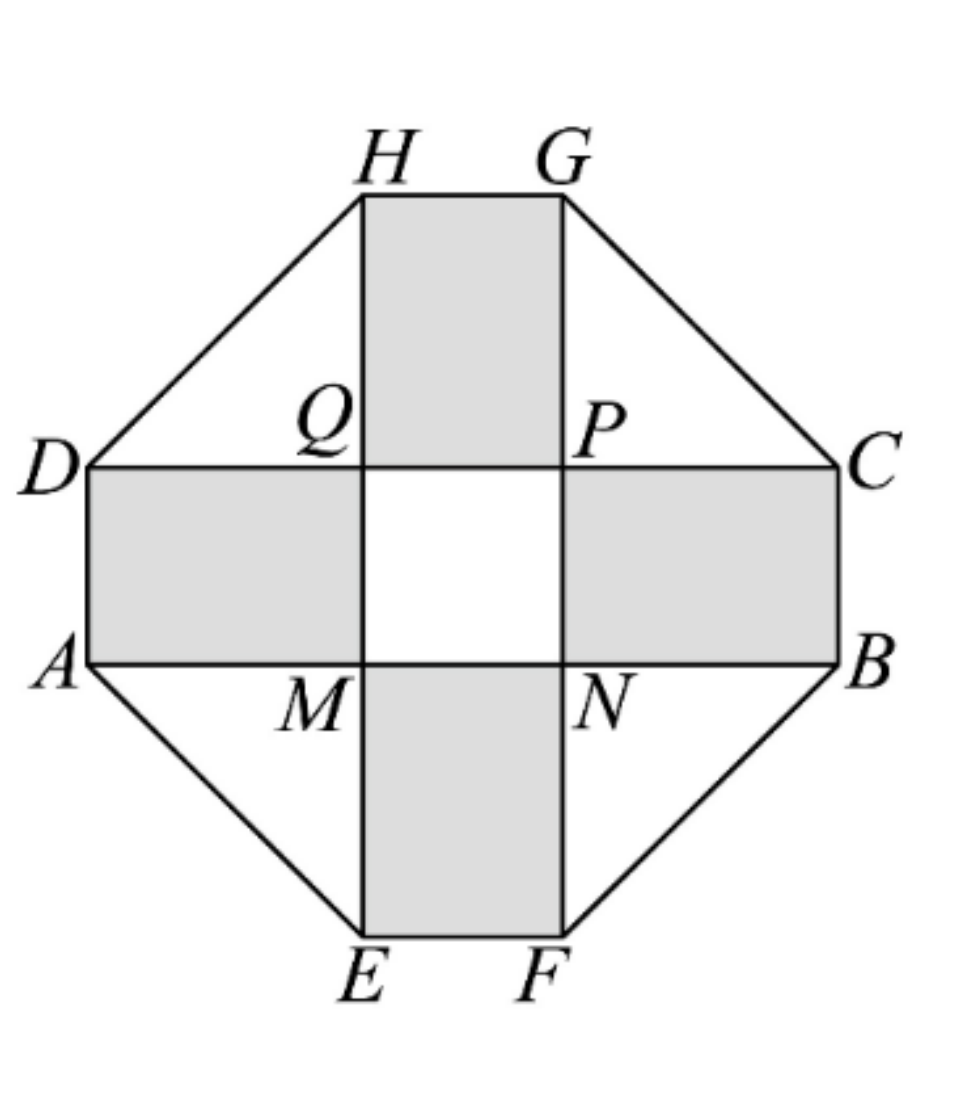
\includegraphics[width=0.34\textwidth]{figures/cross_octagon_h64.png}
\end{center}

\begin{enumerate}[label=(\arabic*)]
\item 设 $DQ$ 长为 $y\mathrm{m}$（$y>0$），用 $x$ 表示 $y$，并求出 $x$ 的取值范围；
\item 如何设计 $AD$ 可使总造价最低，并求出最低造价.
\item 若总造价 $W$ 不超过 69000 元，求 $AD$ 长 $x$ 的取值范围.
\end{enumerate}

\ifanswer
\solbegin
\stepm{(1)}{设 $DQ$ 长为 $y\mathrm{m}$，因为十字形区域面积为 $200\text{m}^2$，}
\step{所以 $4xy+x^2=200$，解得 $y=\dfrac{200-x^2}{4x}=\dfrac{50}{x}-\dfrac x4$；\dots\dots2 分}
\step{因为 $y>0$，所以 $x^2<200$，因为 $x>0$，所以 $0<x<10\sqrt2$.\dots\dots4 分}
\stepm{(2)}{四个矩形地砖面积 $S_{\text{四个矩形}}=4xy=200-x^2$，}
\step{造价 $W_{\text{四个矩形}}=105(200-x^2)$；}
\step{四个三角形草坪面积 $S_{\text{三角形}}=4\times\dfrac12y^2=2\left(\dfrac{50}{x}-\dfrac x4\right)^2=\dfrac{5000}{x^2}+\dfrac{x^2}8-50$，}
\step{造价 $W_{\text{三角形}}=40\left(\dfrac{5000}{x^2}+\dfrac{x^2}8-50\right)$；}
\step{正方形花坛面积 $S_{\text{正方形}}=x^2$，造价 $W_{\text{正方形}}=2100x^2$；}
\step{总造价 $W=W_{\text{四个矩形}}+W_{\text{三角形}}+W_{\text{正方形}}$}
\step{$=105(200-x^2)+40\left(\dfrac{5000}{x^2}+\dfrac{x^2}8-50\right)+2100x^2$，}
\step{化简得 $W=2000x^2+19000+\dfrac{200000}{x^2}$（$0<x<10\sqrt2$）.\dots\dots6 分}
\step{因为 $2000x^2+\dfrac{200000}{x^2}\geqslant40000$，}
\step{当且仅当 $x=\sqrt{10}$（在 $x$ 范围中）时取等号，此时 $W=59000$ 元.}
\step{综上，当 $AD$ 的长为 $\sqrt{10}$ 时，总造价最低，为 59000 元.\dots\dots8 分}
% 原卷 (3) 定义域印作 0<x<2√10，与 (1) 所得 0<x<10√2 不一致，照录（见文件头“原卷笔误”④）
\stepm{(3)}{由（2）得 $W=2000x^2+19000+\dfrac{200000}{x^2}$（$0<x<2\sqrt{10}$）.}
\step{总造价不超过 69000 元，即 $W=2000x^2+19000+\dfrac{200000}{x^2}\leqslant69000$，}
\step{化简得 $x^2+\dfrac{100}{x^2}\leqslant25$，\dots\dots10 分}
\step{即 $(x^2)^2-25x^2+100=(x^2-20)(x^2-5)\leqslant0$，即 $\sqrt5\leqslant x\leqslant2\sqrt5$，}
% 原卷末句“取值范围[√5,2√5]”脱“为”，照录（见文件头“原卷笔误”⑤）
\step{所以 $AD$ 长 $x$ 的取值范围$[\sqrt5,2\sqrt5]$.\dots\dots12 分}
\solend
\fi

\ansspace[10]

\item 设 $a,b,c$ 为实数，集合 $S=\{x\mid(x+a)(x^2+bx+c)=0,x\in\R\}$.

\begin{enumerate}[label=(\arabic*)]
\item 若 $a=1,b=3,c=2$，求集合 $S$；
\item 若 $S=\{-2\}$，求 $a,b,c$ 满足的条件；
\item 设 $T=\{x\mid(ax+1)(cx^2+bx+1)=0,x\in\R\}$，当 $ac\neq0$ 时，如果 $\dfrac12\in S$，$-2\in T$，且
集合 $S,T$ 均恰有两个元素，求三元数对 $(a,b,c)$.
\end{enumerate}

\ifanswer
\solbegin
\stepm{(1)}{若 $a=1,b=3,c=2$，}
\step{则方程 $(x+a)(x^2+bx+c)=0$ 为 $(x+1)(x^2+3x+2)=0$，}
\step{即 $(x+1)^2(x+2)=0$，解得 $x=-1$ 或 $x=-2$，所以 $S=\{-1,-2\}$；}
\stepm{(2)}{由题意得 $-a\in S$，因为 $S=\{-2\}$，所以 $-2$ 是方程 $x+a=0$ 的根，}
\step{即 $-2+a=0$，解得 $a=2$. 由 $S=\{-2\}$，集合 $S$ 有且仅有一个元素，}
\step{即方程 $(x+a)(x^2+bx+c)=0$ 有且仅有一个根，}
\stepm{①}{若 $-2$ 是方程 $x^2+bx+c=0$ 的根，}
\step{则 $\Delta=b^2-4c=0$，且 $-\dfrac b2=-2$，解得 $b=4,c=4$；}
\stepm{②}{若 $-2$ 不是方程 $x^2+bx+c=0$ 的根，则方程 $x^2+bx+c=0$ 无实数根，}
\step{则 $\Delta=b^2-4c<0$，}
\step{综上所述，$\begin{cases}a=2\\ b=4\\ c=4\end{cases}$ 或 $\begin{cases}a=2\\ b^2-4c<0\end{cases}$.}
\stepm{(3)}{$S=\{x\mid(x+a)(x^2+bx+c)=0,x\in\R\}$，}
\step{$T=\{x\mid(ax+1)(cx^2+bx+1)=0,x\in\R\}$，}
\step{由题意得 $a\neq0$ 且 $c\neq0$，则 $-a\in S,-\dfrac1a\in T$，}
\step{且方程 $x^2+bx+c=0$ 与 $cx^2+bx+1=0$ 有相同的判别式 $\Delta=b^2-4c$，}
\step{即两方程根的个数相同. 由集合 $S,T$ 均恰有两个元素，则 $\Delta=b^2-4c\geqslant0$.}
\step{$S=\{x\mid(x+a)(x^2+bx+c)=0,x\in\R\}$，}
\step{因为 $\dfrac12\in S$，所以 $\dfrac12$ 是方程 $x+a=0$ 或 $x^2+bx+c=0$ 的根.}
\step{$T=\{x\mid(ax+1)(cx^2+bx+1)=0,x\in\R\}$，}
\step{由 $-\dfrac1a\in T$，且 $-2\in T$，则 $-2$ 是方程 $ax+1=0$ 或 $cx^2+bx+1=0$ 的根.}
\stepm{①}{当 $a=-\dfrac12$ 时，$\dfrac12$ 是方程 $x+a=0$ 的根，$-a=\dfrac12\in S$，则 $-\dfrac1a=2\in T$，}
\step{又 $-2\in T$，则 $T=\{-2,2\}$，}
\step{由 $T=\left\{x\mid\left(-\dfrac12x+1\right)(cx^2+bx+1)=0,x\in\R\right\}$，}
% 原卷句末为句号，本稿原错作逗号
\step{则 $-2$ 是方程 $cx^2+bx+1=0$ 的根，则 $4c-2b+1=0$.}
\stepm{(i)}{若 $\Delta=b^2-4c=0$，联立 $\begin{cases}4c-2b+1=0\\ b^2-4c=0\end{cases}$ 解得 $b=1,c=\dfrac14$.}
\step{验证：当 $a=-\dfrac12,b=1,c=\dfrac14$ 时，}
\step{$S=\left\{x\mid\left(x-\dfrac12\right)\left(x^2+x+\dfrac14\right)=0,x\in\R\right\}=\left\{-\dfrac12,\dfrac12\right\}$，}
\step{$T=\left\{x\mid\left(-\dfrac12x+1\right)\left(\dfrac14x^2+x+1\right)=0,x\in\R\right\}=\{-2,2\}$，满足题意；}
\stepm{(ii)}{若 $\Delta=b^2-4c>0$，方程 $cx^2+bx+1=0$ 有两个不相等的实数根，}
\step{又 $T=\{-2,2\}$，则方程 $cx^2+bx+1=0$ 的两根必为 $-2$ 和 2.}
\step{由韦达定理得 $\begin{cases}-2+2=-\dfrac bc\\ -2\times2=\dfrac1c\end{cases}$，解得 $b=0,c=-\dfrac14$；}
\step{验证：当 $a=-\dfrac12,b=0,c=-\dfrac14$ 时，}
\step{$S=\left\{x\mid\left(x-\dfrac12\right)\left(x^2-\dfrac14\right)=0,x\in\R\right\}=\left\{-\dfrac12,\dfrac12\right\}$，}
\step{$T=\left\{x\mid\left(-\dfrac12x+1\right)\left(-\dfrac14x^2+1\right)=0,x\in\R\right\}=\{-2,2\}$，满足题意；}
\stepm{②}{当 $a=\dfrac12$ 时，$-\dfrac1a=-2$，即 $-2$ 是方程 $ax+1=0$ 的根，}
\step{则 $-a=-\dfrac12\in S$，又 $\dfrac12\in S$，则 $S=\left\{-\dfrac12,\dfrac12\right\}$，}
\step{$S=\{x\mid(x+a)(x^2+bx+c)=0,x\in\R\}$，}
\step{则 $\dfrac12$ 是方程 $x^2+bx+c=0$ 的根，则 $\dfrac14+\dfrac12b+c=0$，即 $4c+2b+1=0$；}
\stepm{(i)}{若 $\Delta=b^2-4c=0$，联立 $\begin{cases}4c+2b+1=0\\ b^2-4c=0\end{cases}$ 解得 $b=-1,c=\dfrac14$.}
\step{验证：当 $a=\dfrac12,b=-1,c=\dfrac14$ 时，}
\step{$S=\left\{x\mid\left(x+\dfrac12\right)\left(x^2-x+\dfrac14\right)=0,x\in\R\right\}=\left\{-\dfrac12,\dfrac12\right\}$，}
\step{$T=\left\{x\mid\left(\dfrac12x+1\right)\left(\dfrac14x^2-x+1\right)=0,x\in\R\right\}=\{-2,2\}$，满足题意；}
% 原卷作“有两不等的实数根”，本稿原脱“的”
\stepm{(ii)}{若 $\Delta=b^2-4c>0$，方程 $x^2+bx+c=0$ 有两不等的实数根，}
% 原卷句末为句号，本稿原错作逗号
\step{又 $S=\left\{-\dfrac12,\dfrac12\right\}$，则方程 $x^2+bx+c=0$ 的两根必为 $-\dfrac12$ 和 $\dfrac12$.}
\step{由韦达定理得 $\begin{cases}-\dfrac12+\dfrac12=-b\\ -\dfrac12\times\dfrac12=c\end{cases}$，解得 $b=0,c=-\dfrac14$；}
\step{验证：当 $a=\dfrac12,b=0,c=-\dfrac14$ 时，}
\step{$S=\left\{x\mid\left(x+\dfrac12\right)\left(x^2-\dfrac14\right)=0,x\in\R\right\}=\left\{-\dfrac12,\dfrac12\right\}$，}
\step{$T=\left\{x\mid\left(\dfrac12x+1\right)\left(-\dfrac14x^2+1\right)=0,x\in\R\right\}=\{-2,2\}$，满足题意；}
\stepm{③}{当 $a\neq-\dfrac12$ 且 $a\neq\dfrac12$ 时，则 $\dfrac12$ 不是方程 $x+a=0$ 的根，}
\step{$-2$ 也不是方程 $ax+1=0$ 的根.}
% 原卷此句单根而称“两实数根”，语病，照录（见文件头“原卷笔误”⑥）
\step{由 $\dfrac12\in S,-2\in T$，则 $\dfrac12$ 是方程 $x^2+bx+c=0$ 的两实数根，}
\step{且 $-2$ 是方程 $cx^2+bx+1=0$ 的根，则有 $\begin{cases}\dfrac14+\dfrac12b+c=0\\ 4c-2b+1=0\end{cases}$，}
\step{解得 $b=0,c=-\dfrac14$.}
\step{验证：当 $a\neq-\dfrac12$ 且 $a\neq\dfrac12,b=0,c=-\dfrac14$ 时，有 $-a\neq\dfrac12,-a\neq-\dfrac12$.}
\step{$S=\left\{x\mid(x+a)\left(x^2-\dfrac14\right)=0,x\in\R\right\}=\left\{-a,-\dfrac12,\dfrac12\right\}$ 有三个元素，}
\step{故不满足题意；}
\step{综上所述，满足题意的所有三元数对 $(a,b,c)$ 有}
\step{$\left(-\dfrac12,1,\dfrac14\right)$，$\left(-\dfrac12,0,-\dfrac14\right)$，$\left(\dfrac12,-1,\dfrac14\right)$，$\left(\dfrac12,0,-\dfrac14\right)$.}
\solend
\fi

\ansspace*[10]

\end{enumerate}

\end{document}
"
%
% 原始材料：微信公众号“魔都数学加油站”文章，作者破晓，连载“27学年高一64”；
% 原文标题“27学年高一64——2026-2027年上海市格致中学高一上10月月考”；
% 原文链接：https://mp.weixin.qq.com/s/0DfB77nTJf7NdVI_FYXxeA。
% 页面标注发布时间 2026-10-17 21:58（上海）。
% 本次转录只据 `原图/高一64_格致中学_10月月考/` 的 14 张 PNG 逐页读图。
% 正文为 14 张 PNG 页（`01..14.png`）：第 12、13、14 页 2560×3620，
% 第 01—11 页 4762×6735（**同一篇各页分辨率不同**），均按页序读取。
% 14 页全为试卷正文页（卷首标题在第 1 页页顶，卷末解答题第 18 题解析止于第 14 页），
% 无封面页、目录页、二维码或宣传页。粉色斜排“魔都数学加油站”为卷面水印，与公众号页脚一并未录入。
%
% 卷首标题：照卷面印作“2026--2027 年格致中学高一上 10 月月考”，年份区间按全稿惯例排 en dash。
% 原卷只有一行标题、无副标题。
%
% 篇幅与题号：原卷自第 3 题起编号（第 1、2 题不在本卷内）。填空题 3—10（8 题）、
% 选择题 11—14（4 题）、解答题 15—18（4 题），共 16 题。本稿沿用原节与原题号，
% 只改排为全稿统一的大节样式（原卷小节标题为“一、填空题”“二、选择题”“三、解答题”）。
%
% 讲评版：原卷每题下直接印【答案】或【解析】。**只印【答案】的 1 题**（第 5 题），
% 本稿只给 \ans{}；其余 15 题都印【解析】（按全稿口径这类题不另提 \ans{}——第 11、13、14 题
% 的结论写在解析末句（“故选 A”“故选 D”等），亦照录在解析内）。**另有 1 题答案印在题干括号内**——
% 第 12 题（“( B )”，该题无【答案】/【解析】段），本稿按 高一37 第 13 题成例把括号留空、
% 答案另提为 \ans{$B$}。
%
% 副标题：原卷未印副标题。本稿按“知识模块”口径标作“集合与常用逻辑用语、不等式”：
% 16 题中集合与常用逻辑用语 8 题（第 4、9、10、11、12、13、16、18 题），
% 不等式 8 题（含一元二次方程与韦达定理、基本不等式、二次不等式、恒成立、分式不等式：
% 第 3、5、6、7、8、14、15、17 题），两类均达三分之一，故并标。口径同 高一59、高一63。
%
% 与原卷的排版差异：
%   ① 原卷每题下直接印【答案】/【解析】，本稿按全稿惯例将答案与解析置于答案版，试卷版保持干净；
%   ② 原卷未印副标题，本稿按“知识模块”口径补出；
%   ③ 原卷填空横线约三四个字宽，本稿按全稿惯例统一排 \blankline[4.4em]；
%   ④ 原卷实数集排斜体 $R$（第 4、7、8、13、15、18 题）或粗体 $\mathbf{R}$（第 18 题题干与
%      解析共 6 处），整数集排斜体 $Z$（第 9、13 题）或粗体 $\mathbf{Z}$（第 9 题解析末两行），
%      有理数集排粗体 $\mathbf{Q}$（第 13 题选项 A），本稿按全稿惯例统一改用 $\R$、$\Z$、$\Q$
%      （记号归一，粗体／斜体不作区分）；空集记号原卷作 $\varnothing$，照录；
%   ⑤ 第 4 题的补集**原卷用上划线记号 $\bar B$**（题干 1 处、解析 4 处，共 5 处），
%      与全稿惯例的 $\complement_U B$ 不同，本稿照录原卷的 $\bar B$；
%   ⑥ 原卷用描述法时竖线排细竖“$|$”（如 $\{x\mid|x|\geqslant2024\}$ 一类），本稿按全稿惯例排 \mid；
%   ⑦ 第 15—18 题的子问原卷各自另起一行、以“（1）”“（2）”“（3）”标号，本稿按全稿惯例用
%      enumerate 的 (1)(2)(3)；解析中的子问标号一律用 \stepm{(1)}{…}；
%      第 18 题解析中分情形的①②③与分小目的 (i)(ii)，按全稿惯例作 \stepm{①}{…}、\stepm{(i)}{…}；
%   ⑧ 第 13 题解析的“A 选项：”“B 选项：”“C 选项：”“D 选项：”原卷排**加粗**（共 4 处），
%      同 高一63“法一：”成例，本稿排 \stepm{A 选项：}{…} 一类（加粗着色、不改黑色基调），
%      冒号照原卷排全角；
%   ⑨ 第 17 题解析带评分档，原卷在档与档之间排一串点线（“………2 分”），
%      本稿照录为“\dots\dots2 分”一类（同 高一54 成例），共 5 处；
%   ⑩ 选择题的作答括号原卷排半角“(　　)”（第 11、13、14 题括号内空白、第 12 题括号内印 B），
%      本稿按全稿惯例排 \mbox{（\quad）}；选项字母后的句点照原卷排“A.”“B.”；
%   ⑪ 每道解答题原卷未留作答空白，本稿按全稿惯例加 \ansspace（末题用 \ansspace*）；
%   ⑫ 第 17 题题干右侧的十字形八边形示意图，本稿按原卷截图裁出（`figures/cross_octagon_h64.png`，
%      原分辨率裁切，未放大、未用 TikZ 重绘），图内阴影与点名照原卷。
%
% 原卷笔误/存疑（均照录未改，正文对应处另有 % 注）：
%   ① 第 8 题解析末两步自相矛盾：上一步已化为 $\dfrac x{x-1}<0$，下一步却印作
%      “即 $x(x+1)<0$，解得 $-1<x<0$”并给出解集 $(-1,0)$——由 $\dfrac x{x-1}<0$ 应得
%      $x(x-1)<0$、解集 $(0,1)$；已 8 倍放大确认原卷确为 $x+1$ 与 $(-1,0)$，照录未改。
%   ② 第 13 题 D 选项解析“乘法满足结合率”的“率”应为“律”（同段 A、B 选项均作“结合律”）。
%   ③ 第 13 题条件①“任意 $a,b\in G$. 有 $a*b\in G$；”在 $G$ 后印句号（其余三条均以逗号
%      接下文），疑为逗号之误，照录。
%   ④ 第 17 题 (3) 解析把定义域印作 $0<x<2\sqrt{10}$，与 (1) 所得 $0<x<10\sqrt2$ 不一致
%      （疑为 $10\sqrt2$ 之误）；照录未改。
%   ⑤ 第 17 题 (3) 末句“所以 $AD$ 长 $x$ 的取值范围$[\sqrt5,2\sqrt5]$.”脱一个“为”。
%   ⑥ 第 18 题 (3) ③“则 $\dfrac12$ 是方程 $x^2+bx+c=0$ 的**两**实数根”——只有一个数却称
%      “两实数根”，语病；照录。
%
% 插图：第 17 题题干有 1 幅十字形八边形示意图（原卷第 09 页右侧），已按原卷截图排入；
% 其余 13 页无任何图形、无“如图”字样（第 17 题的“图中”均指此图）。
%
\documentclass[a4paper,11pt]{article}
\usepackage{common}

\begin{document}

\examtitlest[3]{2026--2027 年格致中学高一上 10 月月考}{集合与常用逻辑用语、不等式}

\bigsec{一、填空题}

\begin{enumerate}
\setcounter{enumi}{2}

\item 已知一元二次方程 $x^2-nx+5=0$ 的两个实根分别为 $x_1$、$x_2$，且 $\dfrac1{x_1}+\dfrac1{x_2}=1$，则实数 $n$ 的值为\blankline[4.4em].

\ifanswer
\solbegin
\step{$\dfrac1{x_1}+\dfrac1{x_2}=\dfrac{x_1+x_2}{x_1x_2}=\dfrac n5=1$，所以 $n=5$.}
\solend
\fi

\item 全集为 $U=\R$，$A=\{x\mid|x|\geqslant2\}$，$B=\{y\mid y=x^2+1,x\in\R\}$，则 $A\cup\bar B=$\blankline[4.4em].

\ifanswer
\solbegin
\step{由题意得集合 $A=\{x\mid x\geqslant2\text{ 或 }x\leqslant-2\}$，}
\step{因为 $x^2+1\geqslant1$，所以集合 $B=\{x\mid x\geqslant1\}$，所以 $\bar B=\{x\mid x<1\}$，}
\step{则 $A\cup\bar B=\{x\mid x\geqslant2\text{ 或 }x<1\}$.}
\solend
\fi

\item 若 $x>2$，则 $4x+\dfrac1{x-2}$ 的最小值为\blankline[4.4em].

\ifanswer
\ans{$12$}
\fi

\item 已知关于 $x$ 不等式组$\begin{cases}(3x-2)(2x+3)\leqslant0\\ x-a<0\end{cases}$\!没有实数解，则实数 $a$ 的取值范围为\blankline[4.4em].

\ifanswer
\solbegin
\step{由题意得 $\begin{cases}-\dfrac32\leqslant x\leqslant\dfrac23\\ x<a\end{cases}$ 无解，所以 $a\leqslant-\dfrac32$.}
\solend
\fi

\item 若不等式 $\dfrac{x^2-8x+20}{mx^2-mx-1}<0$ 对一切 $x\in\R$ 都成立，则实数 $m$ 的取值范围为\blankline[4.4em].

\ifanswer
\solbegin
\step{因为 $x^2-8x+20=(x-4)^2+4\geqslant4>0$，所以 $mx^2-mx-1<0$，}
\step{当 $m=0$ 时，$mx^2-mx-1=-1<0$，不等式成立；}
\step{设 $y=mx^2-mx-1$，当 $m\neq0$ 时函数 $y$ 为二次函数，$y$ 要恒小于 0，}
\step{抛物线开口向下且与 $x$ 轴没有交点，即 $m<0$ 且 $\Delta<0$，得 $-4<m\leqslant0$，}
\step{故实数 $m$ 的取值范围为 $(-4,0]$.}
\solend
\fi

\item 已知关于 $x$ 的不等式 $\dfrac{ax-1}{x+b}>0$ 的解集为 $\{x\mid-1<x<2\}$，其中 $a$、$b\in\R$，则关于 $x$ 的不等式 $\dfrac{bx+1}{ax+1}<1$ 的解集为\blankline[4.4em].

\ifanswer
\solbegin
\step{不等式 $\dfrac{ax-1}{x+b}>0$ 等价于 $(ax-1)(x+b)>0$，即 $ax^2+(ab-1)x-b>0$，}
\step{所以 $-1$ 和 2 为方程 $ax^2+(ab-1)x-b=0$ 的两根，且 $a<0$，}
\step{由韦达定理得 $\begin{cases}-1+2=-\dfrac{ab-1}a\\ -1\times2=-\dfrac ba\end{cases}$，解得 $\begin{cases}a=-1\\ b=-2\end{cases}$，}
\step{所以原不等式为 $\dfrac{-2x+1}{-x+1}<1\Rightarrow\dfrac{-2x+1}{-x+1}-1<0\Rightarrow\dfrac{-x}{-x+1}<0\Rightarrow\dfrac x{x-1}<0$，}
% 原卷下一步印作“即 x(x+1)<0，解得 -1<x<0”，与上一步 x/(x-1)<0 不等价，
% 照录未改（见文件头“原卷笔误”①）
\step{即 $x(x+1)<0$，解得 $-1<x<0$，即不等式 $\dfrac{bx+1}{ax+1}<1$ 的解集为 $(-1,0)$.}
\solend
\fi

\item 已知集合 $M=\{x\mid|x|\leqslant2024,x\in\Z\}$，集合 $P$ 是 $M$ 的三元子集，即 $P=\{a,b,c\}\subseteq M$，$P$~中元素 $a,b,c$ 满足 $\begin{cases}\dfrac1a+\dfrac1b=\dfrac2c\\ a+c=2b\end{cases}$，则符合要求的集合 $P$ 有\blankline[4.4em]个.

\ifanswer
\solbegin
\step{由 $a+c=2b$，则 $a=2b-c$，代入 $\dfrac1a+\dfrac1b=\dfrac2c$，即 $\dfrac1{2b-c}=\dfrac2c-\dfrac1b=\dfrac{2b-c}{bc}$，}
\step{整理得 $(2b-c)^2=bc$，展开得 $4b^2-5bc+c^2=0$，}
\step{解得 $b=\dfrac c4$ 或 $b=c$（由集合的互异性，舍去），代入 $a+c=2b$ 得 $a=-\dfrac c2$，}
\step{则 $P=\left\{-\dfrac c2,\dfrac c4,c\right\}\subseteq\{x\mid-2024\leqslant x\leqslant2024,x\in\Z\}$，所以 $c$ 为 4 的整数倍，}
\step{且不为 0，则共有 $\dfrac{2024}4\times2=1012$ 个.}
\solend
\fi

\item 已知正整数 $n\geqslant2$，对集合 $\{1,2,3,\cdots,n\}$ 及其每一个非空子集 $X$，记
$X=\{x_1,x_2,\cdots,x_k\}$，其中 $x_1>x_2>\cdots>x_k$，定义一个运算“交替和”
$S_X=x_1-x_2+x_3\cdots+(-1)^{k+1}x_k$. 例如：对于集合 $X=\{9,6,4,2,1\}$，
$S_X=9-6+4-2+1=6$. 则当 $n=7$ 时，集合 $\{1,2,3,\cdots,n\}$ 的所有子集的“交替和”的总
和为\blankline[4.4em].

\ifanswer
\solbegin
\step{由题意得集合 $\{7\}$ 的“交替和”为 7.}
\step{集合 $\{1,2,3,4,5,6,7\}$ 的所有 $2^7$ 个子集中，除去集合 $\{7\}$ 外，}
\step{还有 $2^7-2$ 个非空子集，这 $2^7-2$ 个非空子集中不含元素 7 的集合，}
\step{即 $\{1,2,3,4,5,6\}$ 的非空子集，共有 $2^6-1$ 个，设为 $A_i(i=1,2,\cdots,2^6-1)$；}
\step{则这 $2^7-2$ 个非空子集中含元素 7 的集合，也共有 $2^6-1$ 个，}
\step{这样的集合都可以看成相应地在每个不含 7 的集合中再加上元素 7 得到，}
\step{即 $A_i\cup\{7\}$.}
\step{对 $A_i(i=1,2,\cdots,2^6-1)$ 中的任意集合 $A$，记 $A=\{x_1,x_2,\cdots,x_k\}$，}
\step{则“交替和”$S_A=x_1-x_2+x_3\cdots+(-1)^{k+1}x_k$，其中 $x_1>x_2>\cdots>x_k$，}
\step{由 $7>x_1>x_2>\cdots>x_k$，}
\step{则集合 $A\cup\{7\}$ 的“交替和”为 $7-[x_1-x_2+x_3\cdots+(-1)^{k+1}x_k]$，}
\step{则集合 $A$ 与集合 $A\cup\{7\}$ 的“交替和”之和为 7，下面举例说明：}
\step{如集合 $\{6,5,4,3,2,1\}$ 与集合 $\{7,6,5,4,3,2,1\}$，}
\step{$\{6,5,4,3,2,1\}$ 的“交替和”为 $6-5+4-3+2-1=3$，}
% 原卷此句在页末折为两个印刷行（“……的“交替和”为”／“7-6+5-4+3-2+1=……”），
% 本稿原并作一条，现照原卷拆开（原卷原样两行 / 本稿原错处：并作一行）
\step{$\{7,6,5,4,3,2,1\}$ 的“交替和”为}
\step{$7-6+5-4+3-2+1=7-(6-5+4-3+2-1)=7-3$，}
\step{即集合 $\{6,5,4,3,2,1\}$ 与集合 $\{7,6,5,4,3,2,1\}$ 的“交替和”之和为 7.}
\step{综上，把这 $2^7-2$ 个非空子集两两结组后分别计算每一组中“交替和”之和，}
\step{且每组中“交替和”之和都为 7，共有 $2^6-1$ 组.}
\step{故集合 $\{1,2,3,4,5,6,7\}$ 所有“交替和”之和，}
\step{由各组之和再加集合 $\{7\}$ 的“交替和”7 即可，}
\step{综上所述，当 $n=7$ 时，集合 $\{1,2,3,\cdots,n\}$ 的所有子集的所有“交替和”之和}
\step{为 $7\times(2^6-1)+7=448$.}
\solend
\fi

\end{enumerate}

\bigsec{二、选择题}

\begin{enumerate}
\setcounter{enumi}{10}

\item 若 $a$、$b\in\R$，则“$a<b<0$”是“$a^2>b^2$”的\mbox{（\quad）}条件.

\keepwithprev
A. 充分非必要\qquad B. 必要非充分

C. 充要\qquad D. 既非充分也非必要

\ifanswer
\solbegin
\step{由 $a<b<0\Rightarrow-a>-b>0\Rightarrow(-a)^2>(-b)^2\Rightarrow a^2>b^2$，}
\step{因此由 $a<b<0$ 可以推出 $a^2>b^2$，}
\step{但是当 $a=1$，$b=0$ 时，显然 $a^2>b^2$ 成立，但是 $a<b<0$ 不成立，}
\step{因此由 $a^2>b^2$ 不一定能推出 $a<b<0$，}
\step{因此“$a<b<0$”是“$a^2>b^2$”的充分非必要条件. 故选 $A$.}
\solend
\fi

% 第 12 题答案“B”直接印在题干括号内“(  B  )”，且该题无【答案】/【解析】段；
% 按 高一37 第 13 题的成例括号留空、答案另提为 \ans{}（见文件头）
\item 用反证法证明结论“$a$、$b$、$c$ 至少有一个是正数”时，应假设\mbox{（\quad）}

\keepwithprev
A. $a$、$b$、$c$ 都是正数\qquad B. $a$、$b$、$c$ 都不是正数

C. $a$、$b$、$c$ 至多有一个正数\qquad D. $a$、$b$、$c$ 至多有两个正数

\ifanswer
\ans{$B$}
\fi

\item “群”的概念由数学家伽罗瓦在 19 世纪 30 年代开创，群论虽起源于对代数多项式方程
的研究，但在量子力学、晶体结构学等其他学科中也有十分广泛的应用.“群”的定义是：

设 $G$ 为某种元素组成的一个非空集合，若在 $G$ 内定义一个运算“*”，满足以下条件：

% 原卷条件①在 G 后印句号，疑为逗号之误，照录（见文件头“原卷笔误”③）
①任意 $a,b\in G$. 有 $a*b\in G$；

②如 $a,b,c\in G$，有 $(a*b)*c=a*(b*c)$；

③在 $G$ 中有一个元素 $e$，对任意 $a\in G$，都有 $a*e=e*a=a$，称 $e$ 为 $G$ 的单位元；

④任意 $a\in G$，在 $G$ 中存在唯一确定的 $b$，使 $a*b=b*a=e$，称 $b$ 为 $a$ 的逆元；

此时称 $(G,*)$ 为一个群.

例如实数集 $\R$ 和实数集上的加法运算“+”就构成一个群 $(\R,+)$，其单位元是 0，每一个数
的逆元是其相反数，那么下列说法中，错误的是\mbox{（\quad）}

\keepwithprev
A. $G=\Q$，则 $(G,+)$ 为一个群

B. $G=\{\sqrt2m+\sqrt3n\mid m,n\in\Z\}$，$(G,+)$ 为一个群

C. $G=\{-1,1\}$，则 $(G,\times)$ 为一个群

D. $G=\{x\mid x=2k+1,k\in\Z\}$，则 $(G,\times)$ 为一个群

\ifanswer
\solbegin
\stepm{A 选项：}{有理数的和还是有理数，求和满足结合律，}
\step{设 $a\in\Q$，单位元为 $e$，则 $a+e=a$，故 $e=0$，}
\step{所以每一个数的相反数为其逆元，故 $(G,+)$ 为一个群，选项 A 正确；}
\stepm{B 选项：}{$G=\{\sqrt2m+\sqrt3n\mid m,n\in\Z\}$ 中的任何两个数相加还是属于}
\step{$G=\{\sqrt2m+\sqrt3n\mid m,n\in\Z\}$，求和满足结合律，}
\step{设 $\sqrt2x+\sqrt3y\in G,x,y\in\Z$，单位元为 $e$，}
\step{则 $\sqrt2x+\sqrt3y+e=\sqrt2x+\sqrt3y$，所以 $e=0$，}
\step{每一个数的相反数为其逆元，$(G,+)$ 为一个群，选项 B 正确；}
\stepm{C 选项：}{$G=\{-1,1\}$ 中的两个元素相乘，其积可能为 1 或 $-1$，又 $1\in G,-1\in G$，}
\step{设 $a\in G$，单位元为 $e$，则 $a\times e=a$，故 $e=1,1$ 的逆元为 $1,-1$ 的逆元为 $-1$，}
\step{所以 $(G,\times)$ 为一个群，选项 C 正确；}
% 原卷“乘法满足结合率”的“率”应为“律”（同段 A、B 选项均作“结合律”），照录（见文件头“原卷笔误”②）
\stepm{D 选项：}{两个奇数相乘还是奇数，乘法满足结合率，}
\step{设 $a\in G$，单位元为 $e$，则 $a\times e=a$，故 $e=1$，}
\step{又 $3\in G$，故存在 $b\in G$，使得 $3b=1$，则 $b=\dfrac13$，矛盾，}
\step{故 $(G,\times)$ 不为一个群，选项 D 错误.}
\step{故选 $D$.}
\solend
\fi

\item 已知 $a$、$b$、$c\in\R$，若关于 $x$ 的不等式 $0\leqslant x+\dfrac ax+b\leqslant\dfrac cx-1$ 的解集为 $[x_1,x_2]\cup\{x_3\}$
（$x_3>x_2>x_1>0$），则\mbox{（\quad）}

\keepwithprev
A. 不存在有序数组 $(a,b,c)$，使得 $x_2-x_1=1$

B. 存在唯一有序数组 $(a,b,c)$，使得 $x_2-x_1=1$

C. 有且只有两组有序数组 $(a,b,c)$，使得 $x_2-x_1=1$

D. 存在无穷多组有序数组 $(a,b,c)$，使得 $x_2-x_1=1$

\ifanswer
\solbegin
\step{因为不等式 $0\leqslant x+\dfrac ax+b\leqslant\dfrac cx-1$ 的解集为 $[x_1,x_2]\cup\{x_3\}$（$x_3>x_2>x_1>0$），}
\step{所以 $0\leqslant x^2+bx+a\leqslant c-x$ 在 $[x_1,x_2]\cup\{x_3\}$ 上成立，}
\step{假设 $x_1=m$，$x_2=m+1$，$x_3=n$，}
\step{则 $c-n=0=n^2+bn+a$，由 $x_3$ 为一个独立的数得出，}
\step{所以 $n=c$，且 $m+1$ 与 $n$ 为方程 $x^2+bx+a=0$ 的两个根，}
\step{因为 $x_3>x_2>x_1>0$，所以 $-b=m+n+1=m+c+1$，$a=mn+n=mc+c$，}
\step{所以 $b=-m-c-1$，}
\step{且点 $(x_1,x_1^2+bx_1+a)$ 为 $y=x^2+bx+a$ 与 $y=c-x$ 的左交点，}
\step{所以 $m^2+bm+a=c-m$ 且 $b=-m-c-1$，$a=mc+c$，}
\step{故 $m^2+bm+a=m^2-m^2-mc-m+mc+c=c-m$，所以 $c-m=c-m$ 恒成立，}
\step{所以不论 $a$、$b$、$c$ 取何值，$x_2-x_1=1$ 恒成立，}
\step{即存在无穷多组有序数组 $(a,b,c)$，使得 $x_2-x_1=1$，}
\step{故选项 $A$、$B$、$C$ 错误，选项 $D$ 正确. 故选 $D$.}
\solend
\fi

\end{enumerate}

\bigsec{三、解答题}

\begin{enumerate}
\setcounter{enumi}{14}

\item 已知函数 $f(x)=(a-1)x^2-ax+1$，$a\in\R$.

\begin{enumerate}[label=(\arabic*)]
\item 若不等式 $f(x)<0$ 的解集为 $\left(\dfrac13,1\right)$，求实数 $a$ 的值；
\item 当 $a>1$ 时，解关于 $x$ 的不等式 $f(x)\geqslant0$.
\end{enumerate}

\ifanswer
\solbegin
\stepm{(1)}{因为不等式 $f(x)<0$ 的解集为 $\left(\dfrac13,1\right)$，}
\step{所以不等式对应的方程 $(a-1)x^2-ax+1=0$ 的两根分别为 $\dfrac13$、1，}
\step{由根与系数的关系得 $\begin{cases}1+\dfrac13=\dfrac a{a-1}\\ 1\times\dfrac13=\dfrac1{a-1}\end{cases}$，解得 $a=4$；}
\stepm{(2)}{不等式 $(a-1)x^2-ax+1\geqslant0$（$a>1$）可化为 $(x-1)[(a-1)x-1]\geqslant0$，}
\step{不等式对应方程的两根为 $x_1=1$，$x_2=\dfrac1{a-1}$，}
\step{①当 $\dfrac1{a-1}=1$，即 $a=2$ 时，不等式为 $(x-1)^2\geqslant0$，解集为 $\R$；}
\step{②当 $\dfrac1{a-1}>1$，即 $1<a<2$ 时，解不等式得 $x\leqslant1$ 或 $x\geqslant\dfrac1{a-1}$；}
\step{③当 $\dfrac1{a-1}<1$，即 $a>2$ 时，解不等式得 $x\leqslant\dfrac1{a-1}$ 或 $x\geqslant1$；}
\step{综上，$a=2$ 时，不等式的解集为 $\R$，}
\step{$1<a<2$ 时，不等式的解集为 $(-\infty,1]\cup\left[\dfrac1{a-1},+\infty\right)$，}
\step{$a>2$ 时，不等式的解集为 $\left(-\infty,\dfrac1{a-1}\right]\cup[1,+\infty)$.}
\solend
\fi

\ansspace[6]

\item 若集合 $A=\{x\mid x^2+5x-6=0\}$，$B=\{x\mid x^2+2(m+1)x+m^2-3=0\}$.

\begin{enumerate}[label=(\arabic*)]
\item 若 $m=0$，写出 $A\cup B$ 的子集个数；
\item 若 $A\cap B=B$，求实数 $m$ 的取值范围.
\end{enumerate}

\ifanswer
\solbegin
\stepm{(1)}{当 $m=0$ 时，$B=\{1,-3\}$，}
\step{因为 $A=\{x\mid x^2+5x-6=0\}=\{-6,1\}$，}
\step{所以 $A\cup B=\{-6,-3,1\}$，集合元素个数为 3 个，}
\step{故 $A\cup B$ 的子集个数为 $2^3=8$.}
\stepm{(2)}{因为 $A\cap B=B$，所以 $B\subseteq A$，}
\step{$\Delta=4(m+1)^2-4(m^2-3)=8m+16$，}
\step{当 $\Delta<0$，即 $m<-2$ 时，$B=\varnothing$，符合题意，}
\step{当 $\Delta=0$，即 $m=-2$ 时，$B=\{1\}$，符合题意，}
\step{当 $\Delta>0$，即 $m>-2$ 时，若 $B\subseteq A$，则 $B=\{-6,1\}$，}
\step{即 $\begin{cases}-2(m+1)=-5\\ m^2-3=-6\end{cases}$，方程组无解，}
\step{综上所述，$m$ 的取值范围为 $(-\infty,-2]$.}
\solend
\fi

\ansspace[6]

\item 2025 年上海奇迹花园国际艺术花展于 9 月 20 日正式启幕，本次花展首次实现沉浸 IP
展、花卉景观、跨界艺术、光影夜花园四展合一，为市民游客打造一个可游、可赏、可感
的秋季治愈系童话世界. 某公园受此启发打算设计一个八边形活动区域，该区域的主体造
型平面图是由两个相同的矩形 $ABCD$ 和 $EFGH$ 构成的十字形地域，十字形的面积为
$200\text{m}^2$. 计划在正方形 $MNPQ$ 上建一座花坛，造价为 2100 元$/\text{m}^2$；在四个相同的矩形
（图中阴影部分）上铺地砖，造价为 105 元$/\text{m}^2$；再在四个空角（图中四个三角
形）上铺草坪，造价为 40 元$/\text{m}^2$. 设 $AD$ 长为 $x\mathrm{m}$（$x>0$），总造价为 $W$ 元，求：

\begin{center}
% 插图取自原卷第 09 页右侧截图（原分辨率裁切，未用 TikZ 重绘），阴影与点名照原卷
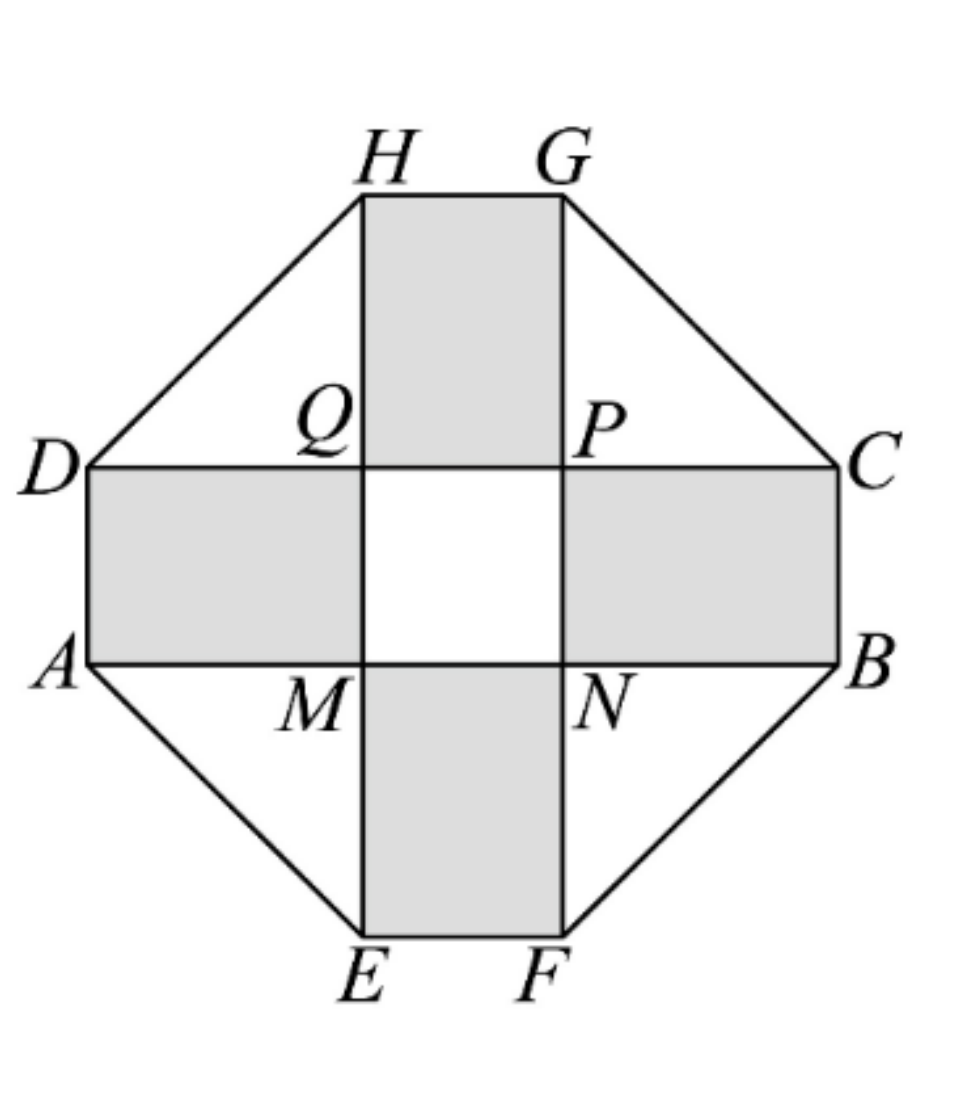
\includegraphics[width=0.34\textwidth]{figures/cross_octagon_h64.png}
\end{center}

\begin{enumerate}[label=(\arabic*)]
\item 设 $DQ$ 长为 $y\mathrm{m}$（$y>0$），用 $x$ 表示 $y$，并求出 $x$ 的取值范围；
\item 如何设计 $AD$ 可使总造价最低，并求出最低造价.
\item 若总造价 $W$ 不超过 69000 元，求 $AD$ 长 $x$ 的取值范围.
\end{enumerate}

\ifanswer
\solbegin
\stepm{(1)}{设 $DQ$ 长为 $y\mathrm{m}$，因为十字形区域面积为 $200\text{m}^2$，}
\step{所以 $4xy+x^2=200$，解得 $y=\dfrac{200-x^2}{4x}=\dfrac{50}{x}-\dfrac x4$；\dots\dots2 分}
\step{因为 $y>0$，所以 $x^2<200$，因为 $x>0$，所以 $0<x<10\sqrt2$.\dots\dots4 分}
\stepm{(2)}{四个矩形地砖面积 $S_{\text{四个矩形}}=4xy=200-x^2$，}
\step{造价 $W_{\text{四个矩形}}=105(200-x^2)$；}
\step{四个三角形草坪面积 $S_{\text{三角形}}=4\times\dfrac12y^2=2\left(\dfrac{50}{x}-\dfrac x4\right)^2=\dfrac{5000}{x^2}+\dfrac{x^2}8-50$，}
\step{造价 $W_{\text{三角形}}=40\left(\dfrac{5000}{x^2}+\dfrac{x^2}8-50\right)$；}
\step{正方形花坛面积 $S_{\text{正方形}}=x^2$，造价 $W_{\text{正方形}}=2100x^2$；}
\step{总造价 $W=W_{\text{四个矩形}}+W_{\text{三角形}}+W_{\text{正方形}}$}
\step{$=105(200-x^2)+40\left(\dfrac{5000}{x^2}+\dfrac{x^2}8-50\right)+2100x^2$，}
\step{化简得 $W=2000x^2+19000+\dfrac{200000}{x^2}$（$0<x<10\sqrt2$）.\dots\dots6 分}
\step{因为 $2000x^2+\dfrac{200000}{x^2}\geqslant40000$，}
\step{当且仅当 $x=\sqrt{10}$（在 $x$ 范围中）时取等号，此时 $W=59000$ 元.}
\step{综上，当 $AD$ 的长为 $\sqrt{10}$ 时，总造价最低，为 59000 元.\dots\dots8 分}
% 原卷 (3) 定义域印作 0<x<2√10，与 (1) 所得 0<x<10√2 不一致，照录（见文件头“原卷笔误”④）
\stepm{(3)}{由（2）得 $W=2000x^2+19000+\dfrac{200000}{x^2}$（$0<x<2\sqrt{10}$）.}
\step{总造价不超过 69000 元，即 $W=2000x^2+19000+\dfrac{200000}{x^2}\leqslant69000$，}
\step{化简得 $x^2+\dfrac{100}{x^2}\leqslant25$，\dots\dots10 分}
\step{即 $(x^2)^2-25x^2+100=(x^2-20)(x^2-5)\leqslant0$，即 $\sqrt5\leqslant x\leqslant2\sqrt5$，}
% 原卷末句“取值范围[√5,2√5]”脱“为”，照录（见文件头“原卷笔误”⑤）
\step{所以 $AD$ 长 $x$ 的取值范围$[\sqrt5,2\sqrt5]$.\dots\dots12 分}
\solend
\fi

\ansspace[10]

\item 设 $a,b,c$ 为实数，集合 $S=\{x\mid(x+a)(x^2+bx+c)=0,x\in\R\}$.

\begin{enumerate}[label=(\arabic*)]
\item 若 $a=1,b=3,c=2$，求集合 $S$；
\item 若 $S=\{-2\}$，求 $a,b,c$ 满足的条件；
\item 设 $T=\{x\mid(ax+1)(cx^2+bx+1)=0,x\in\R\}$，当 $ac\neq0$ 时，如果 $\dfrac12\in S$，$-2\in T$，且
集合 $S,T$ 均恰有两个元素，求三元数对 $(a,b,c)$.
\end{enumerate}

\ifanswer
\solbegin
\stepm{(1)}{若 $a=1,b=3,c=2$，}
\step{则方程 $(x+a)(x^2+bx+c)=0$ 为 $(x+1)(x^2+3x+2)=0$，}
\step{即 $(x+1)^2(x+2)=0$，解得 $x=-1$ 或 $x=-2$，所以 $S=\{-1,-2\}$；}
\stepm{(2)}{由题意得 $-a\in S$，因为 $S=\{-2\}$，所以 $-2$ 是方程 $x+a=0$ 的根，}
\step{即 $-2+a=0$，解得 $a=2$. 由 $S=\{-2\}$，集合 $S$ 有且仅有一个元素，}
\step{即方程 $(x+a)(x^2+bx+c)=0$ 有且仅有一个根，}
\stepm{①}{若 $-2$ 是方程 $x^2+bx+c=0$ 的根，}
\step{则 $\Delta=b^2-4c=0$，且 $-\dfrac b2=-2$，解得 $b=4,c=4$；}
\stepm{②}{若 $-2$ 不是方程 $x^2+bx+c=0$ 的根，则方程 $x^2+bx+c=0$ 无实数根，}
\step{则 $\Delta=b^2-4c<0$，}
\step{综上所述，$\begin{cases}a=2\\ b=4\\ c=4\end{cases}$ 或 $\begin{cases}a=2\\ b^2-4c<0\end{cases}$.}
\stepm{(3)}{$S=\{x\mid(x+a)(x^2+bx+c)=0,x\in\R\}$，}
\step{$T=\{x\mid(ax+1)(cx^2+bx+1)=0,x\in\R\}$，}
\step{由题意得 $a\neq0$ 且 $c\neq0$，则 $-a\in S,-\dfrac1a\in T$，}
\step{且方程 $x^2+bx+c=0$ 与 $cx^2+bx+1=0$ 有相同的判别式 $\Delta=b^2-4c$，}
\step{即两方程根的个数相同. 由集合 $S,T$ 均恰有两个元素，则 $\Delta=b^2-4c\geqslant0$.}
\step{$S=\{x\mid(x+a)(x^2+bx+c)=0,x\in\R\}$，}
\step{因为 $\dfrac12\in S$，所以 $\dfrac12$ 是方程 $x+a=0$ 或 $x^2+bx+c=0$ 的根.}
\step{$T=\{x\mid(ax+1)(cx^2+bx+1)=0,x\in\R\}$，}
\step{由 $-\dfrac1a\in T$，且 $-2\in T$，则 $-2$ 是方程 $ax+1=0$ 或 $cx^2+bx+1=0$ 的根.}
\stepm{①}{当 $a=-\dfrac12$ 时，$\dfrac12$ 是方程 $x+a=0$ 的根，$-a=\dfrac12\in S$，则 $-\dfrac1a=2\in T$，}
\step{又 $-2\in T$，则 $T=\{-2,2\}$，}
\step{由 $T=\left\{x\mid\left(-\dfrac12x+1\right)(cx^2+bx+1)=0,x\in\R\right\}$，}
% 原卷句末为句号，本稿原错作逗号
\step{则 $-2$ 是方程 $cx^2+bx+1=0$ 的根，则 $4c-2b+1=0$.}
\stepm{(i)}{若 $\Delta=b^2-4c=0$，联立 $\begin{cases}4c-2b+1=0\\ b^2-4c=0\end{cases}$ 解得 $b=1,c=\dfrac14$.}
\step{验证：当 $a=-\dfrac12,b=1,c=\dfrac14$ 时，}
\step{$S=\left\{x\mid\left(x-\dfrac12\right)\left(x^2+x+\dfrac14\right)=0,x\in\R\right\}=\left\{-\dfrac12,\dfrac12\right\}$，}
\step{$T=\left\{x\mid\left(-\dfrac12x+1\right)\left(\dfrac14x^2+x+1\right)=0,x\in\R\right\}=\{-2,2\}$，满足题意；}
\stepm{(ii)}{若 $\Delta=b^2-4c>0$，方程 $cx^2+bx+1=0$ 有两个不相等的实数根，}
\step{又 $T=\{-2,2\}$，则方程 $cx^2+bx+1=0$ 的两根必为 $-2$ 和 2.}
\step{由韦达定理得 $\begin{cases}-2+2=-\dfrac bc\\ -2\times2=\dfrac1c\end{cases}$，解得 $b=0,c=-\dfrac14$；}
\step{验证：当 $a=-\dfrac12,b=0,c=-\dfrac14$ 时，}
\step{$S=\left\{x\mid\left(x-\dfrac12\right)\left(x^2-\dfrac14\right)=0,x\in\R\right\}=\left\{-\dfrac12,\dfrac12\right\}$，}
\step{$T=\left\{x\mid\left(-\dfrac12x+1\right)\left(-\dfrac14x^2+1\right)=0,x\in\R\right\}=\{-2,2\}$，满足题意；}
\stepm{②}{当 $a=\dfrac12$ 时，$-\dfrac1a=-2$，即 $-2$ 是方程 $ax+1=0$ 的根，}
\step{则 $-a=-\dfrac12\in S$，又 $\dfrac12\in S$，则 $S=\left\{-\dfrac12,\dfrac12\right\}$，}
\step{$S=\{x\mid(x+a)(x^2+bx+c)=0,x\in\R\}$，}
\step{则 $\dfrac12$ 是方程 $x^2+bx+c=0$ 的根，则 $\dfrac14+\dfrac12b+c=0$，即 $4c+2b+1=0$；}
\stepm{(i)}{若 $\Delta=b^2-4c=0$，联立 $\begin{cases}4c+2b+1=0\\ b^2-4c=0\end{cases}$ 解得 $b=-1,c=\dfrac14$.}
\step{验证：当 $a=\dfrac12,b=-1,c=\dfrac14$ 时，}
\step{$S=\left\{x\mid\left(x+\dfrac12\right)\left(x^2-x+\dfrac14\right)=0,x\in\R\right\}=\left\{-\dfrac12,\dfrac12\right\}$，}
\step{$T=\left\{x\mid\left(\dfrac12x+1\right)\left(\dfrac14x^2-x+1\right)=0,x\in\R\right\}=\{-2,2\}$，满足题意；}
% 原卷作“有两不等的实数根”，本稿原脱“的”
\stepm{(ii)}{若 $\Delta=b^2-4c>0$，方程 $x^2+bx+c=0$ 有两不等的实数根，}
% 原卷句末为句号，本稿原错作逗号
\step{又 $S=\left\{-\dfrac12,\dfrac12\right\}$，则方程 $x^2+bx+c=0$ 的两根必为 $-\dfrac12$ 和 $\dfrac12$.}
\step{由韦达定理得 $\begin{cases}-\dfrac12+\dfrac12=-b\\ -\dfrac12\times\dfrac12=c\end{cases}$，解得 $b=0,c=-\dfrac14$；}
\step{验证：当 $a=\dfrac12,b=0,c=-\dfrac14$ 时，}
\step{$S=\left\{x\mid\left(x+\dfrac12\right)\left(x^2-\dfrac14\right)=0,x\in\R\right\}=\left\{-\dfrac12,\dfrac12\right\}$，}
\step{$T=\left\{x\mid\left(\dfrac12x+1\right)\left(-\dfrac14x^2+1\right)=0,x\in\R\right\}=\{-2,2\}$，满足题意；}
\stepm{③}{当 $a\neq-\dfrac12$ 且 $a\neq\dfrac12$ 时，则 $\dfrac12$ 不是方程 $x+a=0$ 的根，}
\step{$-2$ 也不是方程 $ax+1=0$ 的根.}
% 原卷此句单根而称“两实数根”，语病，照录（见文件头“原卷笔误”⑥）
\step{由 $\dfrac12\in S,-2\in T$，则 $\dfrac12$ 是方程 $x^2+bx+c=0$ 的两实数根，}
\step{且 $-2$ 是方程 $cx^2+bx+1=0$ 的根，则有 $\begin{cases}\dfrac14+\dfrac12b+c=0\\ 4c-2b+1=0\end{cases}$，}
\step{解得 $b=0,c=-\dfrac14$.}
\step{验证：当 $a\neq-\dfrac12$ 且 $a\neq\dfrac12,b=0,c=-\dfrac14$ 时，有 $-a\neq\dfrac12,-a\neq-\dfrac12$.}
\step{$S=\left\{x\mid(x+a)\left(x^2-\dfrac14\right)=0,x\in\R\right\}=\left\{-a,-\dfrac12,\dfrac12\right\}$ 有三个元素，}
\step{故不满足题意；}
\step{综上所述，满足题意的所有三元数对 $(a,b,c)$ 有}
\step{$\left(-\dfrac12,1,\dfrac14\right)$，$\left(-\dfrac12,0,-\dfrac14\right)$，$\left(\dfrac12,-1,\dfrac14\right)$，$\left(\dfrac12,0,-\dfrac14\right)$.}
\solend
\fi

\ansspace*[10]

\end{enumerate}

\end{document}
"
%
% 原始材料：微信公众号“魔都数学加油站”文章，作者破晓，连载“27学年高一64”；
% 原文标题“27学年高一64——2026-2027年上海市格致中学高一上10月月考”；
% 原文链接：https://mp.weixin.qq.com/s/0DfB77nTJf7NdVI_FYXxeA。
% 页面标注发布时间 2026-10-17 21:58（上海）。
% 本次转录只据 `原图/高一64_格致中学_10月月考/` 的 14 张 PNG 逐页读图。
% 正文为 14 张 PNG 页（`01..14.png`）：第 12、13、14 页 2560×3620，
% 第 01—11 页 4762×6735（**同一篇各页分辨率不同**），均按页序读取。
% 14 页全为试卷正文页（卷首标题在第 1 页页顶，卷末解答题第 18 题解析止于第 14 页），
% 无封面页、目录页、二维码或宣传页。粉色斜排“魔都数学加油站”为卷面水印，与公众号页脚一并未录入。
%
% 卷首标题：照卷面印作“2026--2027 年格致中学高一上 10 月月考”，年份区间按全稿惯例排 en dash。
% 原卷只有一行标题、无副标题。
%
% 篇幅与题号：原卷自第 3 题起编号（第 1、2 题不在本卷内）。填空题 3—10（8 题）、
% 选择题 11—14（4 题）、解答题 15—18（4 题），共 16 题。本稿沿用原节与原题号，
% 只改排为全稿统一的大节样式（原卷小节标题为“一、填空题”“二、选择题”“三、解答题”）。
%
% 讲评版：原卷每题下直接印【答案】或【解析】。**只印【答案】的 1 题**（第 5 题），
% 本稿只给 \ans{}；其余 15 题都印【解析】（按全稿口径这类题不另提 \ans{}——第 11、13、14 题
% 的结论写在解析末句（“故选 A”“故选 D”等），亦照录在解析内）。**另有 1 题答案印在题干括号内**——
% 第 12 题（“( B )”，该题无【答案】/【解析】段），本稿按 高一37 第 13 题成例把括号留空、
% 答案另提为 \ans{$B$}。
%
% 副标题：原卷未印副标题。本稿按“知识模块”口径标作“集合与常用逻辑用语、不等式”：
% 16 题中集合与常用逻辑用语 8 题（第 4、9、10、11、12、13、16、18 题），
% 不等式 8 题（含一元二次方程与韦达定理、基本不等式、二次不等式、恒成立、分式不等式：
% 第 3、5、6、7、8、14、15、17 题），两类均达三分之一，故并标。口径同 高一59、高一63。
%
% 与原卷的排版差异：
%   ① 原卷每题下直接印【答案】/【解析】，本稿按全稿惯例将答案与解析置于答案版，试卷版保持干净；
%   ② 原卷未印副标题，本稿按“知识模块”口径补出；
%   ③ 原卷填空横线约三四个字宽，本稿按全稿惯例统一排 \blankline[4.4em]；
%   ④ 原卷实数集排斜体 $R$（第 4、7、8、13、15、18 题）或粗体 $\mathbf{R}$（第 18 题题干与
%      解析共 6 处），整数集排斜体 $Z$（第 9、13 题）或粗体 $\mathbf{Z}$（第 9 题解析末两行），
%      有理数集排粗体 $\mathbf{Q}$（第 13 题选项 A），本稿按全稿惯例统一改用 $\R$、$\Z$、$\Q$
%      （记号归一，粗体／斜体不作区分）；空集记号原卷作 $\varnothing$，照录；
%   ⑤ 第 4 题的补集**原卷用上划线记号 $\bar B$**（题干 1 处、解析 4 处，共 5 处），
%      与全稿惯例的 $\complement_U B$ 不同，本稿照录原卷的 $\bar B$；
%   ⑥ 原卷用描述法时竖线排细竖“$|$”（如 $\{x\mid|x|\geqslant2024\}$ 一类），本稿按全稿惯例排 \mid；
%   ⑦ 第 15—18 题的子问原卷各自另起一行、以“（1）”“（2）”“（3）”标号，本稿按全稿惯例用
%      enumerate 的 (1)(2)(3)；解析中的子问标号一律用 \stepm{(1)}{…}；
%      第 18 题解析中分情形的①②③与分小目的 (i)(ii)，按全稿惯例作 \stepm{①}{…}、\stepm{(i)}{…}；
%   ⑧ 第 13 题解析的“A 选项：”“B 选项：”“C 选项：”“D 选项：”原卷排**加粗**（共 4 处），
%      同 高一63“法一：”成例，本稿排 \stepm{A 选项：}{…} 一类（加粗着色、不改黑色基调），
%      冒号照原卷排全角；
%   ⑨ 第 17 题解析带评分档，原卷在档与档之间排一串点线（“………2 分”），
%      本稿照录为“\dots\dots2 分”一类（同 高一54 成例），共 5 处；
%   ⑩ 选择题的作答括号原卷排半角“(　　)”（第 11、13、14 题括号内空白、第 12 题括号内印 B），
%      本稿按全稿惯例排 \mbox{（\quad）}；选项字母后的句点照原卷排“A.”“B.”；
%   ⑪ 每道解答题原卷未留作答空白，本稿按全稿惯例加 \ansspace（末题用 \ansspace*）；
%   ⑫ 第 17 题题干右侧的十字形八边形示意图，本稿按原卷截图裁出（`figures/cross_octagon_h64.png`，
%      原分辨率裁切，未放大、未用 TikZ 重绘），图内阴影与点名照原卷。
%
% 原卷笔误/存疑（均照录未改，正文对应处另有 % 注）：
%   ① 第 8 题解析末两步自相矛盾：上一步已化为 $\dfrac x{x-1}<0$，下一步却印作
%      “即 $x(x+1)<0$，解得 $-1<x<0$”并给出解集 $(-1,0)$——由 $\dfrac x{x-1}<0$ 应得
%      $x(x-1)<0$、解集 $(0,1)$；已 8 倍放大确认原卷确为 $x+1$ 与 $(-1,0)$，照录未改。
%   ② 第 13 题 D 选项解析“乘法满足结合率”的“率”应为“律”（同段 A、B 选项均作“结合律”）。
%   ③ 第 13 题条件①“任意 $a,b\in G$. 有 $a*b\in G$；”在 $G$ 后印句号（其余三条均以逗号
%      接下文），疑为逗号之误，照录。
%   ④ 第 17 题 (3) 解析把定义域印作 $0<x<2\sqrt{10}$，与 (1) 所得 $0<x<10\sqrt2$ 不一致
%      （疑为 $10\sqrt2$ 之误）；照录未改。
%   ⑤ 第 17 题 (3) 末句“所以 $AD$ 长 $x$ 的取值范围$[\sqrt5,2\sqrt5]$.”脱一个“为”。
%   ⑥ 第 18 题 (3) ③“则 $\dfrac12$ 是方程 $x^2+bx+c=0$ 的**两**实数根”——只有一个数却称
%      “两实数根”，语病；照录。
%
% 插图：第 17 题题干有 1 幅十字形八边形示意图（原卷第 09 页右侧），已按原卷截图排入；
% 其余 13 页无任何图形、无“如图”字样（第 17 题的“图中”均指此图）。
%
\documentclass[a4paper,11pt]{article}
\usepackage{common}

\begin{document}

\examtitlest[3]{2026--2027 年格致中学高一上 10 月月考}{集合与常用逻辑用语、不等式}

\bigsec{一、填空题}

\begin{enumerate}
\setcounter{enumi}{2}

\item 已知一元二次方程 $x^2-nx+5=0$ 的两个实根分别为 $x_1$、$x_2$，且 $\dfrac1{x_1}+\dfrac1{x_2}=1$，则实数 $n$ 的值为\blankline[4.4em].

\ifanswer
\solbegin
\step{$\dfrac1{x_1}+\dfrac1{x_2}=\dfrac{x_1+x_2}{x_1x_2}=\dfrac n5=1$，所以 $n=5$.}
\solend
\fi

\item 全集为 $U=\R$，$A=\{x\mid|x|\geqslant2\}$，$B=\{y\mid y=x^2+1,x\in\R\}$，则 $A\cup\bar B=$\blankline[4.4em].

\ifanswer
\solbegin
\step{由题意得集合 $A=\{x\mid x\geqslant2\text{ 或 }x\leqslant-2\}$，}
\step{因为 $x^2+1\geqslant1$，所以集合 $B=\{x\mid x\geqslant1\}$，所以 $\bar B=\{x\mid x<1\}$，}
\step{则 $A\cup\bar B=\{x\mid x\geqslant2\text{ 或 }x<1\}$.}
\solend
\fi

\item 若 $x>2$，则 $4x+\dfrac1{x-2}$ 的最小值为\blankline[4.4em].

\ifanswer
\ans{$12$}
\fi

\item 已知关于 $x$ 不等式组$\begin{cases}(3x-2)(2x+3)\leqslant0\\ x-a<0\end{cases}$\!没有实数解，则实数 $a$ 的取值范围为\blankline[4.4em].

\ifanswer
\solbegin
\step{由题意得 $\begin{cases}-\dfrac32\leqslant x\leqslant\dfrac23\\ x<a\end{cases}$ 无解，所以 $a\leqslant-\dfrac32$.}
\solend
\fi

\item 若不等式 $\dfrac{x^2-8x+20}{mx^2-mx-1}<0$ 对一切 $x\in\R$ 都成立，则实数 $m$ 的取值范围为\blankline[4.4em].

\ifanswer
\solbegin
\step{因为 $x^2-8x+20=(x-4)^2+4\geqslant4>0$，所以 $mx^2-mx-1<0$，}
\step{当 $m=0$ 时，$mx^2-mx-1=-1<0$，不等式成立；}
\step{设 $y=mx^2-mx-1$，当 $m\neq0$ 时函数 $y$ 为二次函数，$y$ 要恒小于 0，}
\step{抛物线开口向下且与 $x$ 轴没有交点，即 $m<0$ 且 $\Delta<0$，得 $-4<m\leqslant0$，}
\step{故实数 $m$ 的取值范围为 $(-4,0]$.}
\solend
\fi

\item 已知关于 $x$ 的不等式 $\dfrac{ax-1}{x+b}>0$ 的解集为 $\{x\mid-1<x<2\}$，其中 $a$、$b\in\R$，则关于 $x$ 的不等式 $\dfrac{bx+1}{ax+1}<1$ 的解集为\blankline[4.4em].

\ifanswer
\solbegin
\step{不等式 $\dfrac{ax-1}{x+b}>0$ 等价于 $(ax-1)(x+b)>0$，即 $ax^2+(ab-1)x-b>0$，}
\step{所以 $-1$ 和 2 为方程 $ax^2+(ab-1)x-b=0$ 的两根，且 $a<0$，}
\step{由韦达定理得 $\begin{cases}-1+2=-\dfrac{ab-1}a\\ -1\times2=-\dfrac ba\end{cases}$，解得 $\begin{cases}a=-1\\ b=-2\end{cases}$，}
\step{所以原不等式为 $\dfrac{-2x+1}{-x+1}<1\Rightarrow\dfrac{-2x+1}{-x+1}-1<0\Rightarrow\dfrac{-x}{-x+1}<0\Rightarrow\dfrac x{x-1}<0$，}
% 原卷下一步印作“即 x(x+1)<0，解得 -1<x<0”，与上一步 x/(x-1)<0 不等价，
% 照录未改（见文件头“原卷笔误”①）
\step{即 $x(x+1)<0$，解得 $-1<x<0$，即不等式 $\dfrac{bx+1}{ax+1}<1$ 的解集为 $(-1,0)$.}
\solend
\fi

\item 已知集合 $M=\{x\mid|x|\leqslant2024,x\in\Z\}$，集合 $P$ 是 $M$ 的三元子集，即 $P=\{a,b,c\}\subseteq M$，$P$~中元素 $a,b,c$ 满足 $\begin{cases}\dfrac1a+\dfrac1b=\dfrac2c\\ a+c=2b\end{cases}$，则符合要求的集合 $P$ 有\blankline[4.4em]个.

\ifanswer
\solbegin
\step{由 $a+c=2b$，则 $a=2b-c$，代入 $\dfrac1a+\dfrac1b=\dfrac2c$，即 $\dfrac1{2b-c}=\dfrac2c-\dfrac1b=\dfrac{2b-c}{bc}$，}
\step{整理得 $(2b-c)^2=bc$，展开得 $4b^2-5bc+c^2=0$，}
\step{解得 $b=\dfrac c4$ 或 $b=c$（由集合的互异性，舍去），代入 $a+c=2b$ 得 $a=-\dfrac c2$，}
\step{则 $P=\left\{-\dfrac c2,\dfrac c4,c\right\}\subseteq\{x\mid-2024\leqslant x\leqslant2024,x\in\Z\}$，所以 $c$ 为 4 的整数倍，}
\step{且不为 0，则共有 $\dfrac{2024}4\times2=1012$ 个.}
\solend
\fi

\item 已知正整数 $n\geqslant2$，对集合 $\{1,2,3,\cdots,n\}$ 及其每一个非空子集 $X$，记
$X=\{x_1,x_2,\cdots,x_k\}$，其中 $x_1>x_2>\cdots>x_k$，定义一个运算“交替和”
$S_X=x_1-x_2+x_3\cdots+(-1)^{k+1}x_k$. 例如：对于集合 $X=\{9,6,4,2,1\}$，
$S_X=9-6+4-2+1=6$. 则当 $n=7$ 时，集合 $\{1,2,3,\cdots,n\}$ 的所有子集的“交替和”的总
和为\blankline[4.4em].

\ifanswer
\solbegin
\step{由题意得集合 $\{7\}$ 的“交替和”为 7.}
\step{集合 $\{1,2,3,4,5,6,7\}$ 的所有 $2^7$ 个子集中，除去集合 $\{7\}$ 外，}
\step{还有 $2^7-2$ 个非空子集，这 $2^7-2$ 个非空子集中不含元素 7 的集合，}
\step{即 $\{1,2,3,4,5,6\}$ 的非空子集，共有 $2^6-1$ 个，设为 $A_i(i=1,2,\cdots,2^6-1)$；}
\step{则这 $2^7-2$ 个非空子集中含元素 7 的集合，也共有 $2^6-1$ 个，}
\step{这样的集合都可以看成相应地在每个不含 7 的集合中再加上元素 7 得到，}
\step{即 $A_i\cup\{7\}$.}
\step{对 $A_i(i=1,2,\cdots,2^6-1)$ 中的任意集合 $A$，记 $A=\{x_1,x_2,\cdots,x_k\}$，}
\step{则“交替和”$S_A=x_1-x_2+x_3\cdots+(-1)^{k+1}x_k$，其中 $x_1>x_2>\cdots>x_k$，}
\step{由 $7>x_1>x_2>\cdots>x_k$，}
\step{则集合 $A\cup\{7\}$ 的“交替和”为 $7-[x_1-x_2+x_3\cdots+(-1)^{k+1}x_k]$，}
\step{则集合 $A$ 与集合 $A\cup\{7\}$ 的“交替和”之和为 7，下面举例说明：}
\step{如集合 $\{6,5,4,3,2,1\}$ 与集合 $\{7,6,5,4,3,2,1\}$，}
\step{$\{6,5,4,3,2,1\}$ 的“交替和”为 $6-5+4-3+2-1=3$，}
% 原卷此句在页末折为两个印刷行（“……的“交替和”为”／“7-6+5-4+3-2+1=……”），
% 本稿原并作一条，现照原卷拆开（原卷原样两行 / 本稿原错处：并作一行）
\step{$\{7,6,5,4,3,2,1\}$ 的“交替和”为}
\step{$7-6+5-4+3-2+1=7-(6-5+4-3+2-1)=7-3$，}
\step{即集合 $\{6,5,4,3,2,1\}$ 与集合 $\{7,6,5,4,3,2,1\}$ 的“交替和”之和为 7.}
\step{综上，把这 $2^7-2$ 个非空子集两两结组后分别计算每一组中“交替和”之和，}
\step{且每组中“交替和”之和都为 7，共有 $2^6-1$ 组.}
\step{故集合 $\{1,2,3,4,5,6,7\}$ 所有“交替和”之和，}
\step{由各组之和再加集合 $\{7\}$ 的“交替和”7 即可，}
\step{综上所述，当 $n=7$ 时，集合 $\{1,2,3,\cdots,n\}$ 的所有子集的所有“交替和”之和}
\step{为 $7\times(2^6-1)+7=448$.}
\solend
\fi

\end{enumerate}

\bigsec{二、选择题}

\begin{enumerate}
\setcounter{enumi}{10}

\item 若 $a$、$b\in\R$，则“$a<b<0$”是“$a^2>b^2$”的\mbox{（\quad）}条件.

\keepwithprev
A. 充分非必要\qquad B. 必要非充分

C. 充要\qquad D. 既非充分也非必要

\ifanswer
\solbegin
\step{由 $a<b<0\Rightarrow-a>-b>0\Rightarrow(-a)^2>(-b)^2\Rightarrow a^2>b^2$，}
\step{因此由 $a<b<0$ 可以推出 $a^2>b^2$，}
\step{但是当 $a=1$，$b=0$ 时，显然 $a^2>b^2$ 成立，但是 $a<b<0$ 不成立，}
\step{因此由 $a^2>b^2$ 不一定能推出 $a<b<0$，}
\step{因此“$a<b<0$”是“$a^2>b^2$”的充分非必要条件. 故选 $A$.}
\solend
\fi

% 第 12 题答案“B”直接印在题干括号内“(  B  )”，且该题无【答案】/【解析】段；
% 按 高一37 第 13 题的成例括号留空、答案另提为 \ans{}（见文件头）
\item 用反证法证明结论“$a$、$b$、$c$ 至少有一个是正数”时，应假设\mbox{（\quad）}

\keepwithprev
A. $a$、$b$、$c$ 都是正数\qquad B. $a$、$b$、$c$ 都不是正数

C. $a$、$b$、$c$ 至多有一个正数\qquad D. $a$、$b$、$c$ 至多有两个正数

\ifanswer
\ans{$B$}
\fi

\item “群”的概念由数学家伽罗瓦在 19 世纪 30 年代开创，群论虽起源于对代数多项式方程
的研究，但在量子力学、晶体结构学等其他学科中也有十分广泛的应用.“群”的定义是：

设 $G$ 为某种元素组成的一个非空集合，若在 $G$ 内定义一个运算“*”，满足以下条件：

% 原卷条件①在 G 后印句号，疑为逗号之误，照录（见文件头“原卷笔误”③）
①任意 $a,b\in G$. 有 $a*b\in G$；

②如 $a,b,c\in G$，有 $(a*b)*c=a*(b*c)$；

③在 $G$ 中有一个元素 $e$，对任意 $a\in G$，都有 $a*e=e*a=a$，称 $e$ 为 $G$ 的单位元；

④任意 $a\in G$，在 $G$ 中存在唯一确定的 $b$，使 $a*b=b*a=e$，称 $b$ 为 $a$ 的逆元；

此时称 $(G,*)$ 为一个群.

例如实数集 $\R$ 和实数集上的加法运算“+”就构成一个群 $(\R,+)$，其单位元是 0，每一个数
的逆元是其相反数，那么下列说法中，错误的是\mbox{（\quad）}

\keepwithprev
A. $G=\Q$，则 $(G,+)$ 为一个群

B. $G=\{\sqrt2m+\sqrt3n\mid m,n\in\Z\}$，$(G,+)$ 为一个群

C. $G=\{-1,1\}$，则 $(G,\times)$ 为一个群

D. $G=\{x\mid x=2k+1,k\in\Z\}$，则 $(G,\times)$ 为一个群

\ifanswer
\solbegin
\stepm{A 选项：}{有理数的和还是有理数，求和满足结合律，}
\step{设 $a\in\Q$，单位元为 $e$，则 $a+e=a$，故 $e=0$，}
\step{所以每一个数的相反数为其逆元，故 $(G,+)$ 为一个群，选项 A 正确；}
\stepm{B 选项：}{$G=\{\sqrt2m+\sqrt3n\mid m,n\in\Z\}$ 中的任何两个数相加还是属于}
\step{$G=\{\sqrt2m+\sqrt3n\mid m,n\in\Z\}$，求和满足结合律，}
\step{设 $\sqrt2x+\sqrt3y\in G,x,y\in\Z$，单位元为 $e$，}
\step{则 $\sqrt2x+\sqrt3y+e=\sqrt2x+\sqrt3y$，所以 $e=0$，}
\step{每一个数的相反数为其逆元，$(G,+)$ 为一个群，选项 B 正确；}
\stepm{C 选项：}{$G=\{-1,1\}$ 中的两个元素相乘，其积可能为 1 或 $-1$，又 $1\in G,-1\in G$，}
\step{设 $a\in G$，单位元为 $e$，则 $a\times e=a$，故 $e=1,1$ 的逆元为 $1,-1$ 的逆元为 $-1$，}
\step{所以 $(G,\times)$ 为一个群，选项 C 正确；}
% 原卷“乘法满足结合率”的“率”应为“律”（同段 A、B 选项均作“结合律”），照录（见文件头“原卷笔误”②）
\stepm{D 选项：}{两个奇数相乘还是奇数，乘法满足结合率，}
\step{设 $a\in G$，单位元为 $e$，则 $a\times e=a$，故 $e=1$，}
\step{又 $3\in G$，故存在 $b\in G$，使得 $3b=1$，则 $b=\dfrac13$，矛盾，}
\step{故 $(G,\times)$ 不为一个群，选项 D 错误.}
\step{故选 $D$.}
\solend
\fi

\item 已知 $a$、$b$、$c\in\R$，若关于 $x$ 的不等式 $0\leqslant x+\dfrac ax+b\leqslant\dfrac cx-1$ 的解集为 $[x_1,x_2]\cup\{x_3\}$
（$x_3>x_2>x_1>0$），则\mbox{（\quad）}

\keepwithprev
A. 不存在有序数组 $(a,b,c)$，使得 $x_2-x_1=1$

B. 存在唯一有序数组 $(a,b,c)$，使得 $x_2-x_1=1$

C. 有且只有两组有序数组 $(a,b,c)$，使得 $x_2-x_1=1$

D. 存在无穷多组有序数组 $(a,b,c)$，使得 $x_2-x_1=1$

\ifanswer
\solbegin
\step{因为不等式 $0\leqslant x+\dfrac ax+b\leqslant\dfrac cx-1$ 的解集为 $[x_1,x_2]\cup\{x_3\}$（$x_3>x_2>x_1>0$），}
\step{所以 $0\leqslant x^2+bx+a\leqslant c-x$ 在 $[x_1,x_2]\cup\{x_3\}$ 上成立，}
\step{假设 $x_1=m$，$x_2=m+1$，$x_3=n$，}
\step{则 $c-n=0=n^2+bn+a$，由 $x_3$ 为一个独立的数得出，}
\step{所以 $n=c$，且 $m+1$ 与 $n$ 为方程 $x^2+bx+a=0$ 的两个根，}
\step{因为 $x_3>x_2>x_1>0$，所以 $-b=m+n+1=m+c+1$，$a=mn+n=mc+c$，}
\step{所以 $b=-m-c-1$，}
\step{且点 $(x_1,x_1^2+bx_1+a)$ 为 $y=x^2+bx+a$ 与 $y=c-x$ 的左交点，}
\step{所以 $m^2+bm+a=c-m$ 且 $b=-m-c-1$，$a=mc+c$，}
\step{故 $m^2+bm+a=m^2-m^2-mc-m+mc+c=c-m$，所以 $c-m=c-m$ 恒成立，}
\step{所以不论 $a$、$b$、$c$ 取何值，$x_2-x_1=1$ 恒成立，}
\step{即存在无穷多组有序数组 $(a,b,c)$，使得 $x_2-x_1=1$，}
\step{故选项 $A$、$B$、$C$ 错误，选项 $D$ 正确. 故选 $D$.}
\solend
\fi

\end{enumerate}

\bigsec{三、解答题}

\begin{enumerate}
\setcounter{enumi}{14}

\item 已知函数 $f(x)=(a-1)x^2-ax+1$，$a\in\R$.

\begin{enumerate}[label=(\arabic*)]
\item 若不等式 $f(x)<0$ 的解集为 $\left(\dfrac13,1\right)$，求实数 $a$ 的值；
\item 当 $a>1$ 时，解关于 $x$ 的不等式 $f(x)\geqslant0$.
\end{enumerate}

\ifanswer
\solbegin
\stepm{(1)}{因为不等式 $f(x)<0$ 的解集为 $\left(\dfrac13,1\right)$，}
\step{所以不等式对应的方程 $(a-1)x^2-ax+1=0$ 的两根分别为 $\dfrac13$、1，}
\step{由根与系数的关系得 $\begin{cases}1+\dfrac13=\dfrac a{a-1}\\ 1\times\dfrac13=\dfrac1{a-1}\end{cases}$，解得 $a=4$；}
\stepm{(2)}{不等式 $(a-1)x^2-ax+1\geqslant0$（$a>1$）可化为 $(x-1)[(a-1)x-1]\geqslant0$，}
\step{不等式对应方程的两根为 $x_1=1$，$x_2=\dfrac1{a-1}$，}
\step{①当 $\dfrac1{a-1}=1$，即 $a=2$ 时，不等式为 $(x-1)^2\geqslant0$，解集为 $\R$；}
\step{②当 $\dfrac1{a-1}>1$，即 $1<a<2$ 时，解不等式得 $x\leqslant1$ 或 $x\geqslant\dfrac1{a-1}$；}
\step{③当 $\dfrac1{a-1}<1$，即 $a>2$ 时，解不等式得 $x\leqslant\dfrac1{a-1}$ 或 $x\geqslant1$；}
\step{综上，$a=2$ 时，不等式的解集为 $\R$，}
\step{$1<a<2$ 时，不等式的解集为 $(-\infty,1]\cup\left[\dfrac1{a-1},+\infty\right)$，}
\step{$a>2$ 时，不等式的解集为 $\left(-\infty,\dfrac1{a-1}\right]\cup[1,+\infty)$.}
\solend
\fi

\ansspace[6]

\item 若集合 $A=\{x\mid x^2+5x-6=0\}$，$B=\{x\mid x^2+2(m+1)x+m^2-3=0\}$.

\begin{enumerate}[label=(\arabic*)]
\item 若 $m=0$，写出 $A\cup B$ 的子集个数；
\item 若 $A\cap B=B$，求实数 $m$ 的取值范围.
\end{enumerate}

\ifanswer
\solbegin
\stepm{(1)}{当 $m=0$ 时，$B=\{1,-3\}$，}
\step{因为 $A=\{x\mid x^2+5x-6=0\}=\{-6,1\}$，}
\step{所以 $A\cup B=\{-6,-3,1\}$，集合元素个数为 3 个，}
\step{故 $A\cup B$ 的子集个数为 $2^3=8$.}
\stepm{(2)}{因为 $A\cap B=B$，所以 $B\subseteq A$，}
\step{$\Delta=4(m+1)^2-4(m^2-3)=8m+16$，}
\step{当 $\Delta<0$，即 $m<-2$ 时，$B=\varnothing$，符合题意，}
\step{当 $\Delta=0$，即 $m=-2$ 时，$B=\{1\}$，符合题意，}
\step{当 $\Delta>0$，即 $m>-2$ 时，若 $B\subseteq A$，则 $B=\{-6,1\}$，}
\step{即 $\begin{cases}-2(m+1)=-5\\ m^2-3=-6\end{cases}$，方程组无解，}
\step{综上所述，$m$ 的取值范围为 $(-\infty,-2]$.}
\solend
\fi

\ansspace[6]

\item 2025 年上海奇迹花园国际艺术花展于 9 月 20 日正式启幕，本次花展首次实现沉浸 IP
展、花卉景观、跨界艺术、光影夜花园四展合一，为市民游客打造一个可游、可赏、可感
的秋季治愈系童话世界. 某公园受此启发打算设计一个八边形活动区域，该区域的主体造
型平面图是由两个相同的矩形 $ABCD$ 和 $EFGH$ 构成的十字形地域，十字形的面积为
$200\text{m}^2$. 计划在正方形 $MNPQ$ 上建一座花坛，造价为 2100 元$/\text{m}^2$；在四个相同的矩形
（图中阴影部分）上铺地砖，造价为 105 元$/\text{m}^2$；再在四个空角（图中四个三角
形）上铺草坪，造价为 40 元$/\text{m}^2$. 设 $AD$ 长为 $x\mathrm{m}$（$x>0$），总造价为 $W$ 元，求：

\begin{center}
% 插图取自原卷第 09 页右侧截图（原分辨率裁切，未用 TikZ 重绘），阴影与点名照原卷
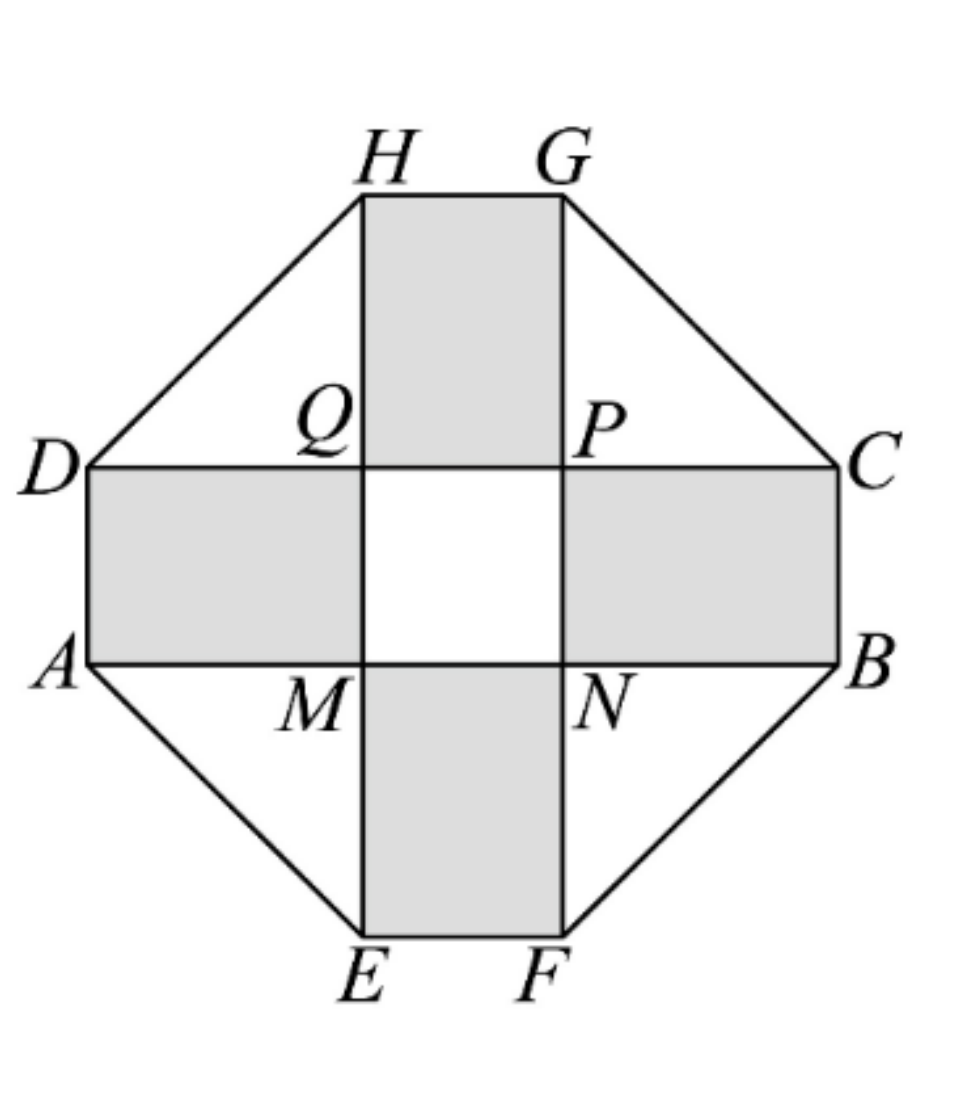
\includegraphics[width=0.34\textwidth]{figures/cross_octagon_h64.png}
\end{center}

\begin{enumerate}[label=(\arabic*)]
\item 设 $DQ$ 长为 $y\mathrm{m}$（$y>0$），用 $x$ 表示 $y$，并求出 $x$ 的取值范围；
\item 如何设计 $AD$ 可使总造价最低，并求出最低造价.
\item 若总造价 $W$ 不超过 69000 元，求 $AD$ 长 $x$ 的取值范围.
\end{enumerate}

\ifanswer
\solbegin
\stepm{(1)}{设 $DQ$ 长为 $y\mathrm{m}$，因为十字形区域面积为 $200\text{m}^2$，}
\step{所以 $4xy+x^2=200$，解得 $y=\dfrac{200-x^2}{4x}=\dfrac{50}{x}-\dfrac x4$；\dots\dots2 分}
\step{因为 $y>0$，所以 $x^2<200$，因为 $x>0$，所以 $0<x<10\sqrt2$.\dots\dots4 分}
\stepm{(2)}{四个矩形地砖面积 $S_{\text{四个矩形}}=4xy=200-x^2$，}
\step{造价 $W_{\text{四个矩形}}=105(200-x^2)$；}
\step{四个三角形草坪面积 $S_{\text{三角形}}=4\times\dfrac12y^2=2\left(\dfrac{50}{x}-\dfrac x4\right)^2=\dfrac{5000}{x^2}+\dfrac{x^2}8-50$，}
\step{造价 $W_{\text{三角形}}=40\left(\dfrac{5000}{x^2}+\dfrac{x^2}8-50\right)$；}
\step{正方形花坛面积 $S_{\text{正方形}}=x^2$，造价 $W_{\text{正方形}}=2100x^2$；}
\step{总造价 $W=W_{\text{四个矩形}}+W_{\text{三角形}}+W_{\text{正方形}}$}
\step{$=105(200-x^2)+40\left(\dfrac{5000}{x^2}+\dfrac{x^2}8-50\right)+2100x^2$，}
\step{化简得 $W=2000x^2+19000+\dfrac{200000}{x^2}$（$0<x<10\sqrt2$）.\dots\dots6 分}
\step{因为 $2000x^2+\dfrac{200000}{x^2}\geqslant40000$，}
\step{当且仅当 $x=\sqrt{10}$（在 $x$ 范围中）时取等号，此时 $W=59000$ 元.}
\step{综上，当 $AD$ 的长为 $\sqrt{10}$ 时，总造价最低，为 59000 元.\dots\dots8 分}
% 原卷 (3) 定义域印作 0<x<2√10，与 (1) 所得 0<x<10√2 不一致，照录（见文件头“原卷笔误”④）
\stepm{(3)}{由（2）得 $W=2000x^2+19000+\dfrac{200000}{x^2}$（$0<x<2\sqrt{10}$）.}
\step{总造价不超过 69000 元，即 $W=2000x^2+19000+\dfrac{200000}{x^2}\leqslant69000$，}
\step{化简得 $x^2+\dfrac{100}{x^2}\leqslant25$，\dots\dots10 分}
\step{即 $(x^2)^2-25x^2+100=(x^2-20)(x^2-5)\leqslant0$，即 $\sqrt5\leqslant x\leqslant2\sqrt5$，}
% 原卷末句“取值范围[√5,2√5]”脱“为”，照录（见文件头“原卷笔误”⑤）
\step{所以 $AD$ 长 $x$ 的取值范围$[\sqrt5,2\sqrt5]$.\dots\dots12 分}
\solend
\fi

\ansspace[10]

\item 设 $a,b,c$ 为实数，集合 $S=\{x\mid(x+a)(x^2+bx+c)=0,x\in\R\}$.

\begin{enumerate}[label=(\arabic*)]
\item 若 $a=1,b=3,c=2$，求集合 $S$；
\item 若 $S=\{-2\}$，求 $a,b,c$ 满足的条件；
\item 设 $T=\{x\mid(ax+1)(cx^2+bx+1)=0,x\in\R\}$，当 $ac\neq0$ 时，如果 $\dfrac12\in S$，$-2\in T$，且
集合 $S,T$ 均恰有两个元素，求三元数对 $(a,b,c)$.
\end{enumerate}

\ifanswer
\solbegin
\stepm{(1)}{若 $a=1,b=3,c=2$，}
\step{则方程 $(x+a)(x^2+bx+c)=0$ 为 $(x+1)(x^2+3x+2)=0$，}
\step{即 $(x+1)^2(x+2)=0$，解得 $x=-1$ 或 $x=-2$，所以 $S=\{-1,-2\}$；}
\stepm{(2)}{由题意得 $-a\in S$，因为 $S=\{-2\}$，所以 $-2$ 是方程 $x+a=0$ 的根，}
\step{即 $-2+a=0$，解得 $a=2$. 由 $S=\{-2\}$，集合 $S$ 有且仅有一个元素，}
\step{即方程 $(x+a)(x^2+bx+c)=0$ 有且仅有一个根，}
\stepm{①}{若 $-2$ 是方程 $x^2+bx+c=0$ 的根，}
\step{则 $\Delta=b^2-4c=0$，且 $-\dfrac b2=-2$，解得 $b=4,c=4$；}
\stepm{②}{若 $-2$ 不是方程 $x^2+bx+c=0$ 的根，则方程 $x^2+bx+c=0$ 无实数根，}
\step{则 $\Delta=b^2-4c<0$，}
\step{综上所述，$\begin{cases}a=2\\ b=4\\ c=4\end{cases}$ 或 $\begin{cases}a=2\\ b^2-4c<0\end{cases}$.}
\stepm{(3)}{$S=\{x\mid(x+a)(x^2+bx+c)=0,x\in\R\}$，}
\step{$T=\{x\mid(ax+1)(cx^2+bx+1)=0,x\in\R\}$，}
\step{由题意得 $a\neq0$ 且 $c\neq0$，则 $-a\in S,-\dfrac1a\in T$，}
\step{且方程 $x^2+bx+c=0$ 与 $cx^2+bx+1=0$ 有相同的判别式 $\Delta=b^2-4c$，}
\step{即两方程根的个数相同. 由集合 $S,T$ 均恰有两个元素，则 $\Delta=b^2-4c\geqslant0$.}
\step{$S=\{x\mid(x+a)(x^2+bx+c)=0,x\in\R\}$，}
\step{因为 $\dfrac12\in S$，所以 $\dfrac12$ 是方程 $x+a=0$ 或 $x^2+bx+c=0$ 的根.}
\step{$T=\{x\mid(ax+1)(cx^2+bx+1)=0,x\in\R\}$，}
\step{由 $-\dfrac1a\in T$，且 $-2\in T$，则 $-2$ 是方程 $ax+1=0$ 或 $cx^2+bx+1=0$ 的根.}
\stepm{①}{当 $a=-\dfrac12$ 时，$\dfrac12$ 是方程 $x+a=0$ 的根，$-a=\dfrac12\in S$，则 $-\dfrac1a=2\in T$，}
\step{又 $-2\in T$，则 $T=\{-2,2\}$，}
\step{由 $T=\left\{x\mid\left(-\dfrac12x+1\right)(cx^2+bx+1)=0,x\in\R\right\}$，}
% 原卷句末为句号，本稿原错作逗号
\step{则 $-2$ 是方程 $cx^2+bx+1=0$ 的根，则 $4c-2b+1=0$.}
\stepm{(i)}{若 $\Delta=b^2-4c=0$，联立 $\begin{cases}4c-2b+1=0\\ b^2-4c=0\end{cases}$ 解得 $b=1,c=\dfrac14$.}
\step{验证：当 $a=-\dfrac12,b=1,c=\dfrac14$ 时，}
\step{$S=\left\{x\mid\left(x-\dfrac12\right)\left(x^2+x+\dfrac14\right)=0,x\in\R\right\}=\left\{-\dfrac12,\dfrac12\right\}$，}
\step{$T=\left\{x\mid\left(-\dfrac12x+1\right)\left(\dfrac14x^2+x+1\right)=0,x\in\R\right\}=\{-2,2\}$，满足题意；}
\stepm{(ii)}{若 $\Delta=b^2-4c>0$，方程 $cx^2+bx+1=0$ 有两个不相等的实数根，}
\step{又 $T=\{-2,2\}$，则方程 $cx^2+bx+1=0$ 的两根必为 $-2$ 和 2.}
\step{由韦达定理得 $\begin{cases}-2+2=-\dfrac bc\\ -2\times2=\dfrac1c\end{cases}$，解得 $b=0,c=-\dfrac14$；}
\step{验证：当 $a=-\dfrac12,b=0,c=-\dfrac14$ 时，}
\step{$S=\left\{x\mid\left(x-\dfrac12\right)\left(x^2-\dfrac14\right)=0,x\in\R\right\}=\left\{-\dfrac12,\dfrac12\right\}$，}
\step{$T=\left\{x\mid\left(-\dfrac12x+1\right)\left(-\dfrac14x^2+1\right)=0,x\in\R\right\}=\{-2,2\}$，满足题意；}
\stepm{②}{当 $a=\dfrac12$ 时，$-\dfrac1a=-2$，即 $-2$ 是方程 $ax+1=0$ 的根，}
\step{则 $-a=-\dfrac12\in S$，又 $\dfrac12\in S$，则 $S=\left\{-\dfrac12,\dfrac12\right\}$，}
\step{$S=\{x\mid(x+a)(x^2+bx+c)=0,x\in\R\}$，}
\step{则 $\dfrac12$ 是方程 $x^2+bx+c=0$ 的根，则 $\dfrac14+\dfrac12b+c=0$，即 $4c+2b+1=0$；}
\stepm{(i)}{若 $\Delta=b^2-4c=0$，联立 $\begin{cases}4c+2b+1=0\\ b^2-4c=0\end{cases}$ 解得 $b=-1,c=\dfrac14$.}
\step{验证：当 $a=\dfrac12,b=-1,c=\dfrac14$ 时，}
\step{$S=\left\{x\mid\left(x+\dfrac12\right)\left(x^2-x+\dfrac14\right)=0,x\in\R\right\}=\left\{-\dfrac12,\dfrac12\right\}$，}
\step{$T=\left\{x\mid\left(\dfrac12x+1\right)\left(\dfrac14x^2-x+1\right)=0,x\in\R\right\}=\{-2,2\}$，满足题意；}
% 原卷作“有两不等的实数根”，本稿原脱“的”
\stepm{(ii)}{若 $\Delta=b^2-4c>0$，方程 $x^2+bx+c=0$ 有两不等的实数根，}
% 原卷句末为句号，本稿原错作逗号
\step{又 $S=\left\{-\dfrac12,\dfrac12\right\}$，则方程 $x^2+bx+c=0$ 的两根必为 $-\dfrac12$ 和 $\dfrac12$.}
\step{由韦达定理得 $\begin{cases}-\dfrac12+\dfrac12=-b\\ -\dfrac12\times\dfrac12=c\end{cases}$，解得 $b=0,c=-\dfrac14$；}
\step{验证：当 $a=\dfrac12,b=0,c=-\dfrac14$ 时，}
\step{$S=\left\{x\mid\left(x+\dfrac12\right)\left(x^2-\dfrac14\right)=0,x\in\R\right\}=\left\{-\dfrac12,\dfrac12\right\}$，}
\step{$T=\left\{x\mid\left(\dfrac12x+1\right)\left(-\dfrac14x^2+1\right)=0,x\in\R\right\}=\{-2,2\}$，满足题意；}
\stepm{③}{当 $a\neq-\dfrac12$ 且 $a\neq\dfrac12$ 时，则 $\dfrac12$ 不是方程 $x+a=0$ 的根，}
\step{$-2$ 也不是方程 $ax+1=0$ 的根.}
% 原卷此句单根而称“两实数根”，语病，照录（见文件头“原卷笔误”⑥）
\step{由 $\dfrac12\in S,-2\in T$，则 $\dfrac12$ 是方程 $x^2+bx+c=0$ 的两实数根，}
\step{且 $-2$ 是方程 $cx^2+bx+1=0$ 的根，则有 $\begin{cases}\dfrac14+\dfrac12b+c=0\\ 4c-2b+1=0\end{cases}$，}
\step{解得 $b=0,c=-\dfrac14$.}
\step{验证：当 $a\neq-\dfrac12$ 且 $a\neq\dfrac12,b=0,c=-\dfrac14$ 时，有 $-a\neq\dfrac12,-a\neq-\dfrac12$.}
\step{$S=\left\{x\mid(x+a)\left(x^2-\dfrac14\right)=0,x\in\R\right\}=\left\{-a,-\dfrac12,\dfrac12\right\}$ 有三个元素，}
\step{故不满足题意；}
\step{综上所述，满足题意的所有三元数对 $(a,b,c)$ 有}
\step{$\left(-\dfrac12,1,\dfrac14\right)$，$\left(-\dfrac12,0,-\dfrac14\right)$，$\left(\dfrac12,-1,\dfrac14\right)$，$\left(\dfrac12,0,-\dfrac14\right)$.}
\solend
\fi

\ansspace*[10]

\end{enumerate}

\end{document}
"
% 紧凑版：xelatex "\def\iscompact{1}% 高一64_格致中学_10月月考.tex
%   —— 高一上数学“2026-2027 年格致中学高一上 10 月月考”（讲评版）
% 试卷版：xelatex 高一64_格致中学_10月月考.tex
% 答案版：xelatex "\def\isanswer{1}% 高一64_格致中学_10月月考.tex
%   —— 高一上数学“2026-2027 年格致中学高一上 10 月月考”（讲评版）
% 试卷版：xelatex 高一64_格致中学_10月月考.tex
% 答案版：xelatex "\def\isanswer{1}% 高一64_格致中学_10月月考.tex
%   —— 高一上数学“2026-2027 年格致中学高一上 10 月月考”（讲评版）
% 试卷版：xelatex 高一64_格致中学_10月月考.tex
% 答案版：xelatex "\def\isanswer{1}\input{高一64_格致中学_10月月考.tex}"
% 紧凑版：xelatex "\def\iscompact{1}\input{高一64_格致中学_10月月考.tex}"
%
% 原始材料：微信公众号“魔都数学加油站”文章，作者破晓，连载“27学年高一64”；
% 原文标题“27学年高一64——2026-2027年上海市格致中学高一上10月月考”；
% 原文链接：https://mp.weixin.qq.com/s/0DfB77nTJf7NdVI_FYXxeA。
% 页面标注发布时间 2026-10-17 21:58（上海）。
% 本次转录只据 `原图/高一64_格致中学_10月月考/` 的 14 张 PNG 逐页读图。
% 正文为 14 张 PNG 页（`01..14.png`）：第 12、13、14 页 2560×3620，
% 第 01—11 页 4762×6735（**同一篇各页分辨率不同**），均按页序读取。
% 14 页全为试卷正文页（卷首标题在第 1 页页顶，卷末解答题第 18 题解析止于第 14 页），
% 无封面页、目录页、二维码或宣传页。粉色斜排“魔都数学加油站”为卷面水印，与公众号页脚一并未录入。
%
% 卷首标题：照卷面印作“2026--2027 年格致中学高一上 10 月月考”，年份区间按全稿惯例排 en dash。
% 原卷只有一行标题、无副标题。
%
% 篇幅与题号：原卷自第 3 题起编号（第 1、2 题不在本卷内）。填空题 3—10（8 题）、
% 选择题 11—14（4 题）、解答题 15—18（4 题），共 16 题。本稿沿用原节与原题号，
% 只改排为全稿统一的大节样式（原卷小节标题为“一、填空题”“二、选择题”“三、解答题”）。
%
% 讲评版：原卷每题下直接印【答案】或【解析】。**只印【答案】的 1 题**（第 5 题），
% 本稿只给 \ans{}；其余 15 题都印【解析】（按全稿口径这类题不另提 \ans{}——第 11、13、14 题
% 的结论写在解析末句（“故选 A”“故选 D”等），亦照录在解析内）。**另有 1 题答案印在题干括号内**——
% 第 12 题（“( B )”，该题无【答案】/【解析】段），本稿按 高一37 第 13 题成例把括号留空、
% 答案另提为 \ans{$B$}。
%
% 副标题：原卷未印副标题。本稿按“知识模块”口径标作“集合与常用逻辑用语、不等式”：
% 16 题中集合与常用逻辑用语 8 题（第 4、9、10、11、12、13、16、18 题），
% 不等式 8 题（含一元二次方程与韦达定理、基本不等式、二次不等式、恒成立、分式不等式：
% 第 3、5、6、7、8、14、15、17 题），两类均达三分之一，故并标。口径同 高一59、高一63。
%
% 与原卷的排版差异：
%   ① 原卷每题下直接印【答案】/【解析】，本稿按全稿惯例将答案与解析置于答案版，试卷版保持干净；
%   ② 原卷未印副标题，本稿按“知识模块”口径补出；
%   ③ 原卷填空横线约三四个字宽，本稿按全稿惯例统一排 \blankline[4.4em]；
%   ④ 原卷实数集排斜体 $R$（第 4、7、8、13、15、18 题）或粗体 $\mathbf{R}$（第 18 题题干与
%      解析共 6 处），整数集排斜体 $Z$（第 9、13 题）或粗体 $\mathbf{Z}$（第 9 题解析末两行），
%      有理数集排粗体 $\mathbf{Q}$（第 13 题选项 A），本稿按全稿惯例统一改用 $\R$、$\Z$、$\Q$
%      （记号归一，粗体／斜体不作区分）；空集记号原卷作 $\varnothing$，照录；
%   ⑤ 第 4 题的补集**原卷用上划线记号 $\bar B$**（题干 1 处、解析 4 处，共 5 处），
%      与全稿惯例的 $\complement_U B$ 不同，本稿照录原卷的 $\bar B$；
%   ⑥ 原卷用描述法时竖线排细竖“$|$”（如 $\{x\mid|x|\geqslant2024\}$ 一类），本稿按全稿惯例排 \mid；
%   ⑦ 第 15—18 题的子问原卷各自另起一行、以“（1）”“（2）”“（3）”标号，本稿按全稿惯例用
%      enumerate 的 (1)(2)(3)；解析中的子问标号一律用 \stepm{(1)}{…}；
%      第 18 题解析中分情形的①②③与分小目的 (i)(ii)，按全稿惯例作 \stepm{①}{…}、\stepm{(i)}{…}；
%   ⑧ 第 13 题解析的“A 选项：”“B 选项：”“C 选项：”“D 选项：”原卷排**加粗**（共 4 处），
%      同 高一63“法一：”成例，本稿排 \stepm{A 选项：}{…} 一类（加粗着色、不改黑色基调），
%      冒号照原卷排全角；
%   ⑨ 第 17 题解析带评分档，原卷在档与档之间排一串点线（“………2 分”），
%      本稿照录为“\dots\dots2 分”一类（同 高一54 成例），共 5 处；
%   ⑩ 选择题的作答括号原卷排半角“(　　)”（第 11、13、14 题括号内空白、第 12 题括号内印 B），
%      本稿按全稿惯例排 \mbox{（\quad）}；选项字母后的句点照原卷排“A.”“B.”；
%   ⑪ 每道解答题原卷未留作答空白，本稿按全稿惯例加 \ansspace（末题用 \ansspace*）；
%   ⑫ 第 17 题题干右侧的十字形八边形示意图，本稿按原卷截图裁出（`figures/cross_octagon_h64.png`，
%      原分辨率裁切，未放大、未用 TikZ 重绘），图内阴影与点名照原卷。
%
% 原卷笔误/存疑（均照录未改，正文对应处另有 % 注）：
%   ① 第 8 题解析末两步自相矛盾：上一步已化为 $\dfrac x{x-1}<0$，下一步却印作
%      “即 $x(x+1)<0$，解得 $-1<x<0$”并给出解集 $(-1,0)$——由 $\dfrac x{x-1}<0$ 应得
%      $x(x-1)<0$、解集 $(0,1)$；已 8 倍放大确认原卷确为 $x+1$ 与 $(-1,0)$，照录未改。
%   ② 第 13 题 D 选项解析“乘法满足结合率”的“率”应为“律”（同段 A、B 选项均作“结合律”）。
%   ③ 第 13 题条件①“任意 $a,b\in G$. 有 $a*b\in G$；”在 $G$ 后印句号（其余三条均以逗号
%      接下文），疑为逗号之误，照录。
%   ④ 第 17 题 (3) 解析把定义域印作 $0<x<2\sqrt{10}$，与 (1) 所得 $0<x<10\sqrt2$ 不一致
%      （疑为 $10\sqrt2$ 之误）；照录未改。
%   ⑤ 第 17 题 (3) 末句“所以 $AD$ 长 $x$ 的取值范围$[\sqrt5,2\sqrt5]$.”脱一个“为”。
%   ⑥ 第 18 题 (3) ③“则 $\dfrac12$ 是方程 $x^2+bx+c=0$ 的**两**实数根”——只有一个数却称
%      “两实数根”，语病；照录。
%
% 插图：第 17 题题干有 1 幅十字形八边形示意图（原卷第 09 页右侧），已按原卷截图排入；
% 其余 13 页无任何图形、无“如图”字样（第 17 题的“图中”均指此图）。
%
\documentclass[a4paper,11pt]{article}
\usepackage{common}

\begin{document}

\examtitlest[3]{2026--2027 年格致中学高一上 10 月月考}{集合与常用逻辑用语、不等式}

\bigsec{一、填空题}

\begin{enumerate}
\setcounter{enumi}{2}

\item 已知一元二次方程 $x^2-nx+5=0$ 的两个实根分别为 $x_1$、$x_2$，且 $\dfrac1{x_1}+\dfrac1{x_2}=1$，则实数 $n$ 的值为\blankline[4.4em].

\ifanswer
\solbegin
\step{$\dfrac1{x_1}+\dfrac1{x_2}=\dfrac{x_1+x_2}{x_1x_2}=\dfrac n5=1$，所以 $n=5$.}
\solend
\fi

\item 全集为 $U=\R$，$A=\{x\mid|x|\geqslant2\}$，$B=\{y\mid y=x^2+1,x\in\R\}$，则 $A\cup\bar B=$\blankline[4.4em].

\ifanswer
\solbegin
\step{由题意得集合 $A=\{x\mid x\geqslant2\text{ 或 }x\leqslant-2\}$，}
\step{因为 $x^2+1\geqslant1$，所以集合 $B=\{x\mid x\geqslant1\}$，所以 $\bar B=\{x\mid x<1\}$，}
\step{则 $A\cup\bar B=\{x\mid x\geqslant2\text{ 或 }x<1\}$.}
\solend
\fi

\item 若 $x>2$，则 $4x+\dfrac1{x-2}$ 的最小值为\blankline[4.4em].

\ifanswer
\ans{$12$}
\fi

\item 已知关于 $x$ 不等式组$\begin{cases}(3x-2)(2x+3)\leqslant0\\ x-a<0\end{cases}$\!没有实数解，则实数 $a$ 的取值范围为\blankline[4.4em].

\ifanswer
\solbegin
\step{由题意得 $\begin{cases}-\dfrac32\leqslant x\leqslant\dfrac23\\ x<a\end{cases}$ 无解，所以 $a\leqslant-\dfrac32$.}
\solend
\fi

\item 若不等式 $\dfrac{x^2-8x+20}{mx^2-mx-1}<0$ 对一切 $x\in\R$ 都成立，则实数 $m$ 的取值范围为\blankline[4.4em].

\ifanswer
\solbegin
\step{因为 $x^2-8x+20=(x-4)^2+4\geqslant4>0$，所以 $mx^2-mx-1<0$，}
\step{当 $m=0$ 时，$mx^2-mx-1=-1<0$，不等式成立；}
\step{设 $y=mx^2-mx-1$，当 $m\neq0$ 时函数 $y$ 为二次函数，$y$ 要恒小于 0，}
\step{抛物线开口向下且与 $x$ 轴没有交点，即 $m<0$ 且 $\Delta<0$，得 $-4<m\leqslant0$，}
\step{故实数 $m$ 的取值范围为 $(-4,0]$.}
\solend
\fi

\item 已知关于 $x$ 的不等式 $\dfrac{ax-1}{x+b}>0$ 的解集为 $\{x\mid-1<x<2\}$，其中 $a$、$b\in\R$，则关于 $x$ 的不等式 $\dfrac{bx+1}{ax+1}<1$ 的解集为\blankline[4.4em].

\ifanswer
\solbegin
\step{不等式 $\dfrac{ax-1}{x+b}>0$ 等价于 $(ax-1)(x+b)>0$，即 $ax^2+(ab-1)x-b>0$，}
\step{所以 $-1$ 和 2 为方程 $ax^2+(ab-1)x-b=0$ 的两根，且 $a<0$，}
\step{由韦达定理得 $\begin{cases}-1+2=-\dfrac{ab-1}a\\ -1\times2=-\dfrac ba\end{cases}$，解得 $\begin{cases}a=-1\\ b=-2\end{cases}$，}
\step{所以原不等式为 $\dfrac{-2x+1}{-x+1}<1\Rightarrow\dfrac{-2x+1}{-x+1}-1<0\Rightarrow\dfrac{-x}{-x+1}<0\Rightarrow\dfrac x{x-1}<0$，}
% 原卷下一步印作“即 x(x+1)<0，解得 -1<x<0”，与上一步 x/(x-1)<0 不等价，
% 照录未改（见文件头“原卷笔误”①）
\step{即 $x(x+1)<0$，解得 $-1<x<0$，即不等式 $\dfrac{bx+1}{ax+1}<1$ 的解集为 $(-1,0)$.}
\solend
\fi

\item 已知集合 $M=\{x\mid|x|\leqslant2024,x\in\Z\}$，集合 $P$ 是 $M$ 的三元子集，即 $P=\{a,b,c\}\subseteq M$，$P$~中元素 $a,b,c$ 满足 $\begin{cases}\dfrac1a+\dfrac1b=\dfrac2c\\ a+c=2b\end{cases}$，则符合要求的集合 $P$ 有\blankline[4.4em]个.

\ifanswer
\solbegin
\step{由 $a+c=2b$，则 $a=2b-c$，代入 $\dfrac1a+\dfrac1b=\dfrac2c$，即 $\dfrac1{2b-c}=\dfrac2c-\dfrac1b=\dfrac{2b-c}{bc}$，}
\step{整理得 $(2b-c)^2=bc$，展开得 $4b^2-5bc+c^2=0$，}
\step{解得 $b=\dfrac c4$ 或 $b=c$（由集合的互异性，舍去），代入 $a+c=2b$ 得 $a=-\dfrac c2$，}
\step{则 $P=\left\{-\dfrac c2,\dfrac c4,c\right\}\subseteq\{x\mid-2024\leqslant x\leqslant2024,x\in\Z\}$，所以 $c$ 为 4 的整数倍，}
\step{且不为 0，则共有 $\dfrac{2024}4\times2=1012$ 个.}
\solend
\fi

\item 已知正整数 $n\geqslant2$，对集合 $\{1,2,3,\cdots,n\}$ 及其每一个非空子集 $X$，记
$X=\{x_1,x_2,\cdots,x_k\}$，其中 $x_1>x_2>\cdots>x_k$，定义一个运算“交替和”
$S_X=x_1-x_2+x_3\cdots+(-1)^{k+1}x_k$. 例如：对于集合 $X=\{9,6,4,2,1\}$，
$S_X=9-6+4-2+1=6$. 则当 $n=7$ 时，集合 $\{1,2,3,\cdots,n\}$ 的所有子集的“交替和”的总
和为\blankline[4.4em].

\ifanswer
\solbegin
\step{由题意得集合 $\{7\}$ 的“交替和”为 7.}
\step{集合 $\{1,2,3,4,5,6,7\}$ 的所有 $2^7$ 个子集中，除去集合 $\{7\}$ 外，}
\step{还有 $2^7-2$ 个非空子集，这 $2^7-2$ 个非空子集中不含元素 7 的集合，}
\step{即 $\{1,2,3,4,5,6\}$ 的非空子集，共有 $2^6-1$ 个，设为 $A_i(i=1,2,\cdots,2^6-1)$；}
\step{则这 $2^7-2$ 个非空子集中含元素 7 的集合，也共有 $2^6-1$ 个，}
\step{这样的集合都可以看成相应地在每个不含 7 的集合中再加上元素 7 得到，}
\step{即 $A_i\cup\{7\}$.}
\step{对 $A_i(i=1,2,\cdots,2^6-1)$ 中的任意集合 $A$，记 $A=\{x_1,x_2,\cdots,x_k\}$，}
\step{则“交替和”$S_A=x_1-x_2+x_3\cdots+(-1)^{k+1}x_k$，其中 $x_1>x_2>\cdots>x_k$，}
\step{由 $7>x_1>x_2>\cdots>x_k$，}
\step{则集合 $A\cup\{7\}$ 的“交替和”为 $7-[x_1-x_2+x_3\cdots+(-1)^{k+1}x_k]$，}
\step{则集合 $A$ 与集合 $A\cup\{7\}$ 的“交替和”之和为 7，下面举例说明：}
\step{如集合 $\{6,5,4,3,2,1\}$ 与集合 $\{7,6,5,4,3,2,1\}$，}
\step{$\{6,5,4,3,2,1\}$ 的“交替和”为 $6-5+4-3+2-1=3$，}
% 原卷此句在页末折为两个印刷行（“……的“交替和”为”／“7-6+5-4+3-2+1=……”），
% 本稿原并作一条，现照原卷拆开（原卷原样两行 / 本稿原错处：并作一行）
\step{$\{7,6,5,4,3,2,1\}$ 的“交替和”为}
\step{$7-6+5-4+3-2+1=7-(6-5+4-3+2-1)=7-3$，}
\step{即集合 $\{6,5,4,3,2,1\}$ 与集合 $\{7,6,5,4,3,2,1\}$ 的“交替和”之和为 7.}
\step{综上，把这 $2^7-2$ 个非空子集两两结组后分别计算每一组中“交替和”之和，}
\step{且每组中“交替和”之和都为 7，共有 $2^6-1$ 组.}
\step{故集合 $\{1,2,3,4,5,6,7\}$ 所有“交替和”之和，}
\step{由各组之和再加集合 $\{7\}$ 的“交替和”7 即可，}
\step{综上所述，当 $n=7$ 时，集合 $\{1,2,3,\cdots,n\}$ 的所有子集的所有“交替和”之和}
\step{为 $7\times(2^6-1)+7=448$.}
\solend
\fi

\end{enumerate}

\bigsec{二、选择题}

\begin{enumerate}
\setcounter{enumi}{10}

\item 若 $a$、$b\in\R$，则“$a<b<0$”是“$a^2>b^2$”的\mbox{（\quad）}条件.

\keepwithprev
A. 充分非必要\qquad B. 必要非充分

C. 充要\qquad D. 既非充分也非必要

\ifanswer
\solbegin
\step{由 $a<b<0\Rightarrow-a>-b>0\Rightarrow(-a)^2>(-b)^2\Rightarrow a^2>b^2$，}
\step{因此由 $a<b<0$ 可以推出 $a^2>b^2$，}
\step{但是当 $a=1$，$b=0$ 时，显然 $a^2>b^2$ 成立，但是 $a<b<0$ 不成立，}
\step{因此由 $a^2>b^2$ 不一定能推出 $a<b<0$，}
\step{因此“$a<b<0$”是“$a^2>b^2$”的充分非必要条件. 故选 $A$.}
\solend
\fi

% 第 12 题答案“B”直接印在题干括号内“(  B  )”，且该题无【答案】/【解析】段；
% 按 高一37 第 13 题的成例括号留空、答案另提为 \ans{}（见文件头）
\item 用反证法证明结论“$a$、$b$、$c$ 至少有一个是正数”时，应假设\mbox{（\quad）}

\keepwithprev
A. $a$、$b$、$c$ 都是正数\qquad B. $a$、$b$、$c$ 都不是正数

C. $a$、$b$、$c$ 至多有一个正数\qquad D. $a$、$b$、$c$ 至多有两个正数

\ifanswer
\ans{$B$}
\fi

\item “群”的概念由数学家伽罗瓦在 19 世纪 30 年代开创，群论虽起源于对代数多项式方程
的研究，但在量子力学、晶体结构学等其他学科中也有十分广泛的应用.“群”的定义是：

设 $G$ 为某种元素组成的一个非空集合，若在 $G$ 内定义一个运算“*”，满足以下条件：

% 原卷条件①在 G 后印句号，疑为逗号之误，照录（见文件头“原卷笔误”③）
①任意 $a,b\in G$. 有 $a*b\in G$；

②如 $a,b,c\in G$，有 $(a*b)*c=a*(b*c)$；

③在 $G$ 中有一个元素 $e$，对任意 $a\in G$，都有 $a*e=e*a=a$，称 $e$ 为 $G$ 的单位元；

④任意 $a\in G$，在 $G$ 中存在唯一确定的 $b$，使 $a*b=b*a=e$，称 $b$ 为 $a$ 的逆元；

此时称 $(G,*)$ 为一个群.

例如实数集 $\R$ 和实数集上的加法运算“+”就构成一个群 $(\R,+)$，其单位元是 0，每一个数
的逆元是其相反数，那么下列说法中，错误的是\mbox{（\quad）}

\keepwithprev
A. $G=\Q$，则 $(G,+)$ 为一个群

B. $G=\{\sqrt2m+\sqrt3n\mid m,n\in\Z\}$，$(G,+)$ 为一个群

C. $G=\{-1,1\}$，则 $(G,\times)$ 为一个群

D. $G=\{x\mid x=2k+1,k\in\Z\}$，则 $(G,\times)$ 为一个群

\ifanswer
\solbegin
\stepm{A 选项：}{有理数的和还是有理数，求和满足结合律，}
\step{设 $a\in\Q$，单位元为 $e$，则 $a+e=a$，故 $e=0$，}
\step{所以每一个数的相反数为其逆元，故 $(G,+)$ 为一个群，选项 A 正确；}
\stepm{B 选项：}{$G=\{\sqrt2m+\sqrt3n\mid m,n\in\Z\}$ 中的任何两个数相加还是属于}
\step{$G=\{\sqrt2m+\sqrt3n\mid m,n\in\Z\}$，求和满足结合律，}
\step{设 $\sqrt2x+\sqrt3y\in G,x,y\in\Z$，单位元为 $e$，}
\step{则 $\sqrt2x+\sqrt3y+e=\sqrt2x+\sqrt3y$，所以 $e=0$，}
\step{每一个数的相反数为其逆元，$(G,+)$ 为一个群，选项 B 正确；}
\stepm{C 选项：}{$G=\{-1,1\}$ 中的两个元素相乘，其积可能为 1 或 $-1$，又 $1\in G,-1\in G$，}
\step{设 $a\in G$，单位元为 $e$，则 $a\times e=a$，故 $e=1,1$ 的逆元为 $1,-1$ 的逆元为 $-1$，}
\step{所以 $(G,\times)$ 为一个群，选项 C 正确；}
% 原卷“乘法满足结合率”的“率”应为“律”（同段 A、B 选项均作“结合律”），照录（见文件头“原卷笔误”②）
\stepm{D 选项：}{两个奇数相乘还是奇数，乘法满足结合率，}
\step{设 $a\in G$，单位元为 $e$，则 $a\times e=a$，故 $e=1$，}
\step{又 $3\in G$，故存在 $b\in G$，使得 $3b=1$，则 $b=\dfrac13$，矛盾，}
\step{故 $(G,\times)$ 不为一个群，选项 D 错误.}
\step{故选 $D$.}
\solend
\fi

\item 已知 $a$、$b$、$c\in\R$，若关于 $x$ 的不等式 $0\leqslant x+\dfrac ax+b\leqslant\dfrac cx-1$ 的解集为 $[x_1,x_2]\cup\{x_3\}$
（$x_3>x_2>x_1>0$），则\mbox{（\quad）}

\keepwithprev
A. 不存在有序数组 $(a,b,c)$，使得 $x_2-x_1=1$

B. 存在唯一有序数组 $(a,b,c)$，使得 $x_2-x_1=1$

C. 有且只有两组有序数组 $(a,b,c)$，使得 $x_2-x_1=1$

D. 存在无穷多组有序数组 $(a,b,c)$，使得 $x_2-x_1=1$

\ifanswer
\solbegin
\step{因为不等式 $0\leqslant x+\dfrac ax+b\leqslant\dfrac cx-1$ 的解集为 $[x_1,x_2]\cup\{x_3\}$（$x_3>x_2>x_1>0$），}
\step{所以 $0\leqslant x^2+bx+a\leqslant c-x$ 在 $[x_1,x_2]\cup\{x_3\}$ 上成立，}
\step{假设 $x_1=m$，$x_2=m+1$，$x_3=n$，}
\step{则 $c-n=0=n^2+bn+a$，由 $x_3$ 为一个独立的数得出，}
\step{所以 $n=c$，且 $m+1$ 与 $n$ 为方程 $x^2+bx+a=0$ 的两个根，}
\step{因为 $x_3>x_2>x_1>0$，所以 $-b=m+n+1=m+c+1$，$a=mn+n=mc+c$，}
\step{所以 $b=-m-c-1$，}
\step{且点 $(x_1,x_1^2+bx_1+a)$ 为 $y=x^2+bx+a$ 与 $y=c-x$ 的左交点，}
\step{所以 $m^2+bm+a=c-m$ 且 $b=-m-c-1$，$a=mc+c$，}
\step{故 $m^2+bm+a=m^2-m^2-mc-m+mc+c=c-m$，所以 $c-m=c-m$ 恒成立，}
\step{所以不论 $a$、$b$、$c$ 取何值，$x_2-x_1=1$ 恒成立，}
\step{即存在无穷多组有序数组 $(a,b,c)$，使得 $x_2-x_1=1$，}
\step{故选项 $A$、$B$、$C$ 错误，选项 $D$ 正确. 故选 $D$.}
\solend
\fi

\end{enumerate}

\bigsec{三、解答题}

\begin{enumerate}
\setcounter{enumi}{14}

\item 已知函数 $f(x)=(a-1)x^2-ax+1$，$a\in\R$.

\begin{enumerate}[label=(\arabic*)]
\item 若不等式 $f(x)<0$ 的解集为 $\left(\dfrac13,1\right)$，求实数 $a$ 的值；
\item 当 $a>1$ 时，解关于 $x$ 的不等式 $f(x)\geqslant0$.
\end{enumerate}

\ifanswer
\solbegin
\stepm{(1)}{因为不等式 $f(x)<0$ 的解集为 $\left(\dfrac13,1\right)$，}
\step{所以不等式对应的方程 $(a-1)x^2-ax+1=0$ 的两根分别为 $\dfrac13$、1，}
\step{由根与系数的关系得 $\begin{cases}1+\dfrac13=\dfrac a{a-1}\\ 1\times\dfrac13=\dfrac1{a-1}\end{cases}$，解得 $a=4$；}
\stepm{(2)}{不等式 $(a-1)x^2-ax+1\geqslant0$（$a>1$）可化为 $(x-1)[(a-1)x-1]\geqslant0$，}
\step{不等式对应方程的两根为 $x_1=1$，$x_2=\dfrac1{a-1}$，}
\step{①当 $\dfrac1{a-1}=1$，即 $a=2$ 时，不等式为 $(x-1)^2\geqslant0$，解集为 $\R$；}
\step{②当 $\dfrac1{a-1}>1$，即 $1<a<2$ 时，解不等式得 $x\leqslant1$ 或 $x\geqslant\dfrac1{a-1}$；}
\step{③当 $\dfrac1{a-1}<1$，即 $a>2$ 时，解不等式得 $x\leqslant\dfrac1{a-1}$ 或 $x\geqslant1$；}
\step{综上，$a=2$ 时，不等式的解集为 $\R$，}
\step{$1<a<2$ 时，不等式的解集为 $(-\infty,1]\cup\left[\dfrac1{a-1},+\infty\right)$，}
\step{$a>2$ 时，不等式的解集为 $\left(-\infty,\dfrac1{a-1}\right]\cup[1,+\infty)$.}
\solend
\fi

\ansspace[6]

\item 若集合 $A=\{x\mid x^2+5x-6=0\}$，$B=\{x\mid x^2+2(m+1)x+m^2-3=0\}$.

\begin{enumerate}[label=(\arabic*)]
\item 若 $m=0$，写出 $A\cup B$ 的子集个数；
\item 若 $A\cap B=B$，求实数 $m$ 的取值范围.
\end{enumerate}

\ifanswer
\solbegin
\stepm{(1)}{当 $m=0$ 时，$B=\{1,-3\}$，}
\step{因为 $A=\{x\mid x^2+5x-6=0\}=\{-6,1\}$，}
\step{所以 $A\cup B=\{-6,-3,1\}$，集合元素个数为 3 个，}
\step{故 $A\cup B$ 的子集个数为 $2^3=8$.}
\stepm{(2)}{因为 $A\cap B=B$，所以 $B\subseteq A$，}
\step{$\Delta=4(m+1)^2-4(m^2-3)=8m+16$，}
\step{当 $\Delta<0$，即 $m<-2$ 时，$B=\varnothing$，符合题意，}
\step{当 $\Delta=0$，即 $m=-2$ 时，$B=\{1\}$，符合题意，}
\step{当 $\Delta>0$，即 $m>-2$ 时，若 $B\subseteq A$，则 $B=\{-6,1\}$，}
\step{即 $\begin{cases}-2(m+1)=-5\\ m^2-3=-6\end{cases}$，方程组无解，}
\step{综上所述，$m$ 的取值范围为 $(-\infty,-2]$.}
\solend
\fi

\ansspace[6]

\item 2025 年上海奇迹花园国际艺术花展于 9 月 20 日正式启幕，本次花展首次实现沉浸 IP
展、花卉景观、跨界艺术、光影夜花园四展合一，为市民游客打造一个可游、可赏、可感
的秋季治愈系童话世界. 某公园受此启发打算设计一个八边形活动区域，该区域的主体造
型平面图是由两个相同的矩形 $ABCD$ 和 $EFGH$ 构成的十字形地域，十字形的面积为
$200\text{m}^2$. 计划在正方形 $MNPQ$ 上建一座花坛，造价为 2100 元$/\text{m}^2$；在四个相同的矩形
（图中阴影部分）上铺地砖，造价为 105 元$/\text{m}^2$；再在四个空角（图中四个三角
形）上铺草坪，造价为 40 元$/\text{m}^2$. 设 $AD$ 长为 $x\mathrm{m}$（$x>0$），总造价为 $W$ 元，求：

\begin{center}
% 插图取自原卷第 09 页右侧截图（原分辨率裁切，未用 TikZ 重绘），阴影与点名照原卷
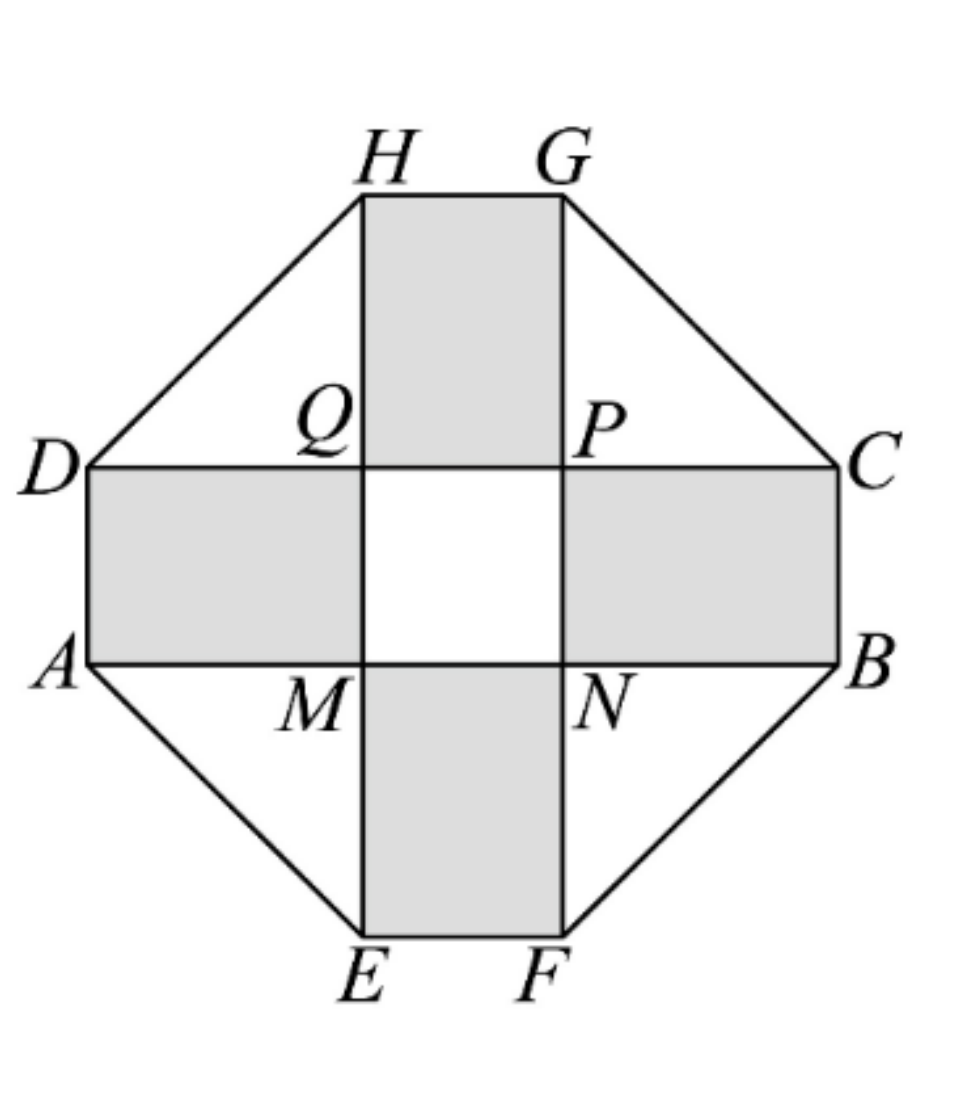
\includegraphics[width=0.34\textwidth]{figures/cross_octagon_h64.png}
\end{center}

\begin{enumerate}[label=(\arabic*)]
\item 设 $DQ$ 长为 $y\mathrm{m}$（$y>0$），用 $x$ 表示 $y$，并求出 $x$ 的取值范围；
\item 如何设计 $AD$ 可使总造价最低，并求出最低造价.
\item 若总造价 $W$ 不超过 69000 元，求 $AD$ 长 $x$ 的取值范围.
\end{enumerate}

\ifanswer
\solbegin
\stepm{(1)}{设 $DQ$ 长为 $y\mathrm{m}$，因为十字形区域面积为 $200\text{m}^2$，}
\step{所以 $4xy+x^2=200$，解得 $y=\dfrac{200-x^2}{4x}=\dfrac{50}{x}-\dfrac x4$；\dots\dots2 分}
\step{因为 $y>0$，所以 $x^2<200$，因为 $x>0$，所以 $0<x<10\sqrt2$.\dots\dots4 分}
\stepm{(2)}{四个矩形地砖面积 $S_{\text{四个矩形}}=4xy=200-x^2$，}
\step{造价 $W_{\text{四个矩形}}=105(200-x^2)$；}
\step{四个三角形草坪面积 $S_{\text{三角形}}=4\times\dfrac12y^2=2\left(\dfrac{50}{x}-\dfrac x4\right)^2=\dfrac{5000}{x^2}+\dfrac{x^2}8-50$，}
\step{造价 $W_{\text{三角形}}=40\left(\dfrac{5000}{x^2}+\dfrac{x^2}8-50\right)$；}
\step{正方形花坛面积 $S_{\text{正方形}}=x^2$，造价 $W_{\text{正方形}}=2100x^2$；}
\step{总造价 $W=W_{\text{四个矩形}}+W_{\text{三角形}}+W_{\text{正方形}}$}
\step{$=105(200-x^2)+40\left(\dfrac{5000}{x^2}+\dfrac{x^2}8-50\right)+2100x^2$，}
\step{化简得 $W=2000x^2+19000+\dfrac{200000}{x^2}$（$0<x<10\sqrt2$）.\dots\dots6 分}
\step{因为 $2000x^2+\dfrac{200000}{x^2}\geqslant40000$，}
\step{当且仅当 $x=\sqrt{10}$（在 $x$ 范围中）时取等号，此时 $W=59000$ 元.}
\step{综上，当 $AD$ 的长为 $\sqrt{10}$ 时，总造价最低，为 59000 元.\dots\dots8 分}
% 原卷 (3) 定义域印作 0<x<2√10，与 (1) 所得 0<x<10√2 不一致，照录（见文件头“原卷笔误”④）
\stepm{(3)}{由（2）得 $W=2000x^2+19000+\dfrac{200000}{x^2}$（$0<x<2\sqrt{10}$）.}
\step{总造价不超过 69000 元，即 $W=2000x^2+19000+\dfrac{200000}{x^2}\leqslant69000$，}
\step{化简得 $x^2+\dfrac{100}{x^2}\leqslant25$，\dots\dots10 分}
\step{即 $(x^2)^2-25x^2+100=(x^2-20)(x^2-5)\leqslant0$，即 $\sqrt5\leqslant x\leqslant2\sqrt5$，}
% 原卷末句“取值范围[√5,2√5]”脱“为”，照录（见文件头“原卷笔误”⑤）
\step{所以 $AD$ 长 $x$ 的取值范围$[\sqrt5,2\sqrt5]$.\dots\dots12 分}
\solend
\fi

\ansspace[10]

\item 设 $a,b,c$ 为实数，集合 $S=\{x\mid(x+a)(x^2+bx+c)=0,x\in\R\}$.

\begin{enumerate}[label=(\arabic*)]
\item 若 $a=1,b=3,c=2$，求集合 $S$；
\item 若 $S=\{-2\}$，求 $a,b,c$ 满足的条件；
\item 设 $T=\{x\mid(ax+1)(cx^2+bx+1)=0,x\in\R\}$，当 $ac\neq0$ 时，如果 $\dfrac12\in S$，$-2\in T$，且
集合 $S,T$ 均恰有两个元素，求三元数对 $(a,b,c)$.
\end{enumerate}

\ifanswer
\solbegin
\stepm{(1)}{若 $a=1,b=3,c=2$，}
\step{则方程 $(x+a)(x^2+bx+c)=0$ 为 $(x+1)(x^2+3x+2)=0$，}
\step{即 $(x+1)^2(x+2)=0$，解得 $x=-1$ 或 $x=-2$，所以 $S=\{-1,-2\}$；}
\stepm{(2)}{由题意得 $-a\in S$，因为 $S=\{-2\}$，所以 $-2$ 是方程 $x+a=0$ 的根，}
\step{即 $-2+a=0$，解得 $a=2$. 由 $S=\{-2\}$，集合 $S$ 有且仅有一个元素，}
\step{即方程 $(x+a)(x^2+bx+c)=0$ 有且仅有一个根，}
\stepm{①}{若 $-2$ 是方程 $x^2+bx+c=0$ 的根，}
\step{则 $\Delta=b^2-4c=0$，且 $-\dfrac b2=-2$，解得 $b=4,c=4$；}
\stepm{②}{若 $-2$ 不是方程 $x^2+bx+c=0$ 的根，则方程 $x^2+bx+c=0$ 无实数根，}
\step{则 $\Delta=b^2-4c<0$，}
\step{综上所述，$\begin{cases}a=2\\ b=4\\ c=4\end{cases}$ 或 $\begin{cases}a=2\\ b^2-4c<0\end{cases}$.}
\stepm{(3)}{$S=\{x\mid(x+a)(x^2+bx+c)=0,x\in\R\}$，}
\step{$T=\{x\mid(ax+1)(cx^2+bx+1)=0,x\in\R\}$，}
\step{由题意得 $a\neq0$ 且 $c\neq0$，则 $-a\in S,-\dfrac1a\in T$，}
\step{且方程 $x^2+bx+c=0$ 与 $cx^2+bx+1=0$ 有相同的判别式 $\Delta=b^2-4c$，}
\step{即两方程根的个数相同. 由集合 $S,T$ 均恰有两个元素，则 $\Delta=b^2-4c\geqslant0$.}
\step{$S=\{x\mid(x+a)(x^2+bx+c)=0,x\in\R\}$，}
\step{因为 $\dfrac12\in S$，所以 $\dfrac12$ 是方程 $x+a=0$ 或 $x^2+bx+c=0$ 的根.}
\step{$T=\{x\mid(ax+1)(cx^2+bx+1)=0,x\in\R\}$，}
\step{由 $-\dfrac1a\in T$，且 $-2\in T$，则 $-2$ 是方程 $ax+1=0$ 或 $cx^2+bx+1=0$ 的根.}
\stepm{①}{当 $a=-\dfrac12$ 时，$\dfrac12$ 是方程 $x+a=0$ 的根，$-a=\dfrac12\in S$，则 $-\dfrac1a=2\in T$，}
\step{又 $-2\in T$，则 $T=\{-2,2\}$，}
\step{由 $T=\left\{x\mid\left(-\dfrac12x+1\right)(cx^2+bx+1)=0,x\in\R\right\}$，}
% 原卷句末为句号，本稿原错作逗号
\step{则 $-2$ 是方程 $cx^2+bx+1=0$ 的根，则 $4c-2b+1=0$.}
\stepm{(i)}{若 $\Delta=b^2-4c=0$，联立 $\begin{cases}4c-2b+1=0\\ b^2-4c=0\end{cases}$ 解得 $b=1,c=\dfrac14$.}
\step{验证：当 $a=-\dfrac12,b=1,c=\dfrac14$ 时，}
\step{$S=\left\{x\mid\left(x-\dfrac12\right)\left(x^2+x+\dfrac14\right)=0,x\in\R\right\}=\left\{-\dfrac12,\dfrac12\right\}$，}
\step{$T=\left\{x\mid\left(-\dfrac12x+1\right)\left(\dfrac14x^2+x+1\right)=0,x\in\R\right\}=\{-2,2\}$，满足题意；}
\stepm{(ii)}{若 $\Delta=b^2-4c>0$，方程 $cx^2+bx+1=0$ 有两个不相等的实数根，}
\step{又 $T=\{-2,2\}$，则方程 $cx^2+bx+1=0$ 的两根必为 $-2$ 和 2.}
\step{由韦达定理得 $\begin{cases}-2+2=-\dfrac bc\\ -2\times2=\dfrac1c\end{cases}$，解得 $b=0,c=-\dfrac14$；}
\step{验证：当 $a=-\dfrac12,b=0,c=-\dfrac14$ 时，}
\step{$S=\left\{x\mid\left(x-\dfrac12\right)\left(x^2-\dfrac14\right)=0,x\in\R\right\}=\left\{-\dfrac12,\dfrac12\right\}$，}
\step{$T=\left\{x\mid\left(-\dfrac12x+1\right)\left(-\dfrac14x^2+1\right)=0,x\in\R\right\}=\{-2,2\}$，满足题意；}
\stepm{②}{当 $a=\dfrac12$ 时，$-\dfrac1a=-2$，即 $-2$ 是方程 $ax+1=0$ 的根，}
\step{则 $-a=-\dfrac12\in S$，又 $\dfrac12\in S$，则 $S=\left\{-\dfrac12,\dfrac12\right\}$，}
\step{$S=\{x\mid(x+a)(x^2+bx+c)=0,x\in\R\}$，}
\step{则 $\dfrac12$ 是方程 $x^2+bx+c=0$ 的根，则 $\dfrac14+\dfrac12b+c=0$，即 $4c+2b+1=0$；}
\stepm{(i)}{若 $\Delta=b^2-4c=0$，联立 $\begin{cases}4c+2b+1=0\\ b^2-4c=0\end{cases}$ 解得 $b=-1,c=\dfrac14$.}
\step{验证：当 $a=\dfrac12,b=-1,c=\dfrac14$ 时，}
\step{$S=\left\{x\mid\left(x+\dfrac12\right)\left(x^2-x+\dfrac14\right)=0,x\in\R\right\}=\left\{-\dfrac12,\dfrac12\right\}$，}
\step{$T=\left\{x\mid\left(\dfrac12x+1\right)\left(\dfrac14x^2-x+1\right)=0,x\in\R\right\}=\{-2,2\}$，满足题意；}
% 原卷作“有两不等的实数根”，本稿原脱“的”
\stepm{(ii)}{若 $\Delta=b^2-4c>0$，方程 $x^2+bx+c=0$ 有两不等的实数根，}
% 原卷句末为句号，本稿原错作逗号
\step{又 $S=\left\{-\dfrac12,\dfrac12\right\}$，则方程 $x^2+bx+c=0$ 的两根必为 $-\dfrac12$ 和 $\dfrac12$.}
\step{由韦达定理得 $\begin{cases}-\dfrac12+\dfrac12=-b\\ -\dfrac12\times\dfrac12=c\end{cases}$，解得 $b=0,c=-\dfrac14$；}
\step{验证：当 $a=\dfrac12,b=0,c=-\dfrac14$ 时，}
\step{$S=\left\{x\mid\left(x+\dfrac12\right)\left(x^2-\dfrac14\right)=0,x\in\R\right\}=\left\{-\dfrac12,\dfrac12\right\}$，}
\step{$T=\left\{x\mid\left(\dfrac12x+1\right)\left(-\dfrac14x^2+1\right)=0,x\in\R\right\}=\{-2,2\}$，满足题意；}
\stepm{③}{当 $a\neq-\dfrac12$ 且 $a\neq\dfrac12$ 时，则 $\dfrac12$ 不是方程 $x+a=0$ 的根，}
\step{$-2$ 也不是方程 $ax+1=0$ 的根.}
% 原卷此句单根而称“两实数根”，语病，照录（见文件头“原卷笔误”⑥）
\step{由 $\dfrac12\in S,-2\in T$，则 $\dfrac12$ 是方程 $x^2+bx+c=0$ 的两实数根，}
\step{且 $-2$ 是方程 $cx^2+bx+1=0$ 的根，则有 $\begin{cases}\dfrac14+\dfrac12b+c=0\\ 4c-2b+1=0\end{cases}$，}
\step{解得 $b=0,c=-\dfrac14$.}
\step{验证：当 $a\neq-\dfrac12$ 且 $a\neq\dfrac12,b=0,c=-\dfrac14$ 时，有 $-a\neq\dfrac12,-a\neq-\dfrac12$.}
\step{$S=\left\{x\mid(x+a)\left(x^2-\dfrac14\right)=0,x\in\R\right\}=\left\{-a,-\dfrac12,\dfrac12\right\}$ 有三个元素，}
\step{故不满足题意；}
\step{综上所述，满足题意的所有三元数对 $(a,b,c)$ 有}
\step{$\left(-\dfrac12,1,\dfrac14\right)$，$\left(-\dfrac12,0,-\dfrac14\right)$，$\left(\dfrac12,-1,\dfrac14\right)$，$\left(\dfrac12,0,-\dfrac14\right)$.}
\solend
\fi

\ansspace*[10]

\end{enumerate}

\end{document}
"
% 紧凑版：xelatex "\def\iscompact{1}% 高一64_格致中学_10月月考.tex
%   —— 高一上数学“2026-2027 年格致中学高一上 10 月月考”（讲评版）
% 试卷版：xelatex 高一64_格致中学_10月月考.tex
% 答案版：xelatex "\def\isanswer{1}\input{高一64_格致中学_10月月考.tex}"
% 紧凑版：xelatex "\def\iscompact{1}\input{高一64_格致中学_10月月考.tex}"
%
% 原始材料：微信公众号“魔都数学加油站”文章，作者破晓，连载“27学年高一64”；
% 原文标题“27学年高一64——2026-2027年上海市格致中学高一上10月月考”；
% 原文链接：https://mp.weixin.qq.com/s/0DfB77nTJf7NdVI_FYXxeA。
% 页面标注发布时间 2026-10-17 21:58（上海）。
% 本次转录只据 `原图/高一64_格致中学_10月月考/` 的 14 张 PNG 逐页读图。
% 正文为 14 张 PNG 页（`01..14.png`）：第 12、13、14 页 2560×3620，
% 第 01—11 页 4762×6735（**同一篇各页分辨率不同**），均按页序读取。
% 14 页全为试卷正文页（卷首标题在第 1 页页顶，卷末解答题第 18 题解析止于第 14 页），
% 无封面页、目录页、二维码或宣传页。粉色斜排“魔都数学加油站”为卷面水印，与公众号页脚一并未录入。
%
% 卷首标题：照卷面印作“2026--2027 年格致中学高一上 10 月月考”，年份区间按全稿惯例排 en dash。
% 原卷只有一行标题、无副标题。
%
% 篇幅与题号：原卷自第 3 题起编号（第 1、2 题不在本卷内）。填空题 3—10（8 题）、
% 选择题 11—14（4 题）、解答题 15—18（4 题），共 16 题。本稿沿用原节与原题号，
% 只改排为全稿统一的大节样式（原卷小节标题为“一、填空题”“二、选择题”“三、解答题”）。
%
% 讲评版：原卷每题下直接印【答案】或【解析】。**只印【答案】的 1 题**（第 5 题），
% 本稿只给 \ans{}；其余 15 题都印【解析】（按全稿口径这类题不另提 \ans{}——第 11、13、14 题
% 的结论写在解析末句（“故选 A”“故选 D”等），亦照录在解析内）。**另有 1 题答案印在题干括号内**——
% 第 12 题（“( B )”，该题无【答案】/【解析】段），本稿按 高一37 第 13 题成例把括号留空、
% 答案另提为 \ans{$B$}。
%
% 副标题：原卷未印副标题。本稿按“知识模块”口径标作“集合与常用逻辑用语、不等式”：
% 16 题中集合与常用逻辑用语 8 题（第 4、9、10、11、12、13、16、18 题），
% 不等式 8 题（含一元二次方程与韦达定理、基本不等式、二次不等式、恒成立、分式不等式：
% 第 3、5、6、7、8、14、15、17 题），两类均达三分之一，故并标。口径同 高一59、高一63。
%
% 与原卷的排版差异：
%   ① 原卷每题下直接印【答案】/【解析】，本稿按全稿惯例将答案与解析置于答案版，试卷版保持干净；
%   ② 原卷未印副标题，本稿按“知识模块”口径补出；
%   ③ 原卷填空横线约三四个字宽，本稿按全稿惯例统一排 \blankline[4.4em]；
%   ④ 原卷实数集排斜体 $R$（第 4、7、8、13、15、18 题）或粗体 $\mathbf{R}$（第 18 题题干与
%      解析共 6 处），整数集排斜体 $Z$（第 9、13 题）或粗体 $\mathbf{Z}$（第 9 题解析末两行），
%      有理数集排粗体 $\mathbf{Q}$（第 13 题选项 A），本稿按全稿惯例统一改用 $\R$、$\Z$、$\Q$
%      （记号归一，粗体／斜体不作区分）；空集记号原卷作 $\varnothing$，照录；
%   ⑤ 第 4 题的补集**原卷用上划线记号 $\bar B$**（题干 1 处、解析 4 处，共 5 处），
%      与全稿惯例的 $\complement_U B$ 不同，本稿照录原卷的 $\bar B$；
%   ⑥ 原卷用描述法时竖线排细竖“$|$”（如 $\{x\mid|x|\geqslant2024\}$ 一类），本稿按全稿惯例排 \mid；
%   ⑦ 第 15—18 题的子问原卷各自另起一行、以“（1）”“（2）”“（3）”标号，本稿按全稿惯例用
%      enumerate 的 (1)(2)(3)；解析中的子问标号一律用 \stepm{(1)}{…}；
%      第 18 题解析中分情形的①②③与分小目的 (i)(ii)，按全稿惯例作 \stepm{①}{…}、\stepm{(i)}{…}；
%   ⑧ 第 13 题解析的“A 选项：”“B 选项：”“C 选项：”“D 选项：”原卷排**加粗**（共 4 处），
%      同 高一63“法一：”成例，本稿排 \stepm{A 选项：}{…} 一类（加粗着色、不改黑色基调），
%      冒号照原卷排全角；
%   ⑨ 第 17 题解析带评分档，原卷在档与档之间排一串点线（“………2 分”），
%      本稿照录为“\dots\dots2 分”一类（同 高一54 成例），共 5 处；
%   ⑩ 选择题的作答括号原卷排半角“(　　)”（第 11、13、14 题括号内空白、第 12 题括号内印 B），
%      本稿按全稿惯例排 \mbox{（\quad）}；选项字母后的句点照原卷排“A.”“B.”；
%   ⑪ 每道解答题原卷未留作答空白，本稿按全稿惯例加 \ansspace（末题用 \ansspace*）；
%   ⑫ 第 17 题题干右侧的十字形八边形示意图，本稿按原卷截图裁出（`figures/cross_octagon_h64.png`，
%      原分辨率裁切，未放大、未用 TikZ 重绘），图内阴影与点名照原卷。
%
% 原卷笔误/存疑（均照录未改，正文对应处另有 % 注）：
%   ① 第 8 题解析末两步自相矛盾：上一步已化为 $\dfrac x{x-1}<0$，下一步却印作
%      “即 $x(x+1)<0$，解得 $-1<x<0$”并给出解集 $(-1,0)$——由 $\dfrac x{x-1}<0$ 应得
%      $x(x-1)<0$、解集 $(0,1)$；已 8 倍放大确认原卷确为 $x+1$ 与 $(-1,0)$，照录未改。
%   ② 第 13 题 D 选项解析“乘法满足结合率”的“率”应为“律”（同段 A、B 选项均作“结合律”）。
%   ③ 第 13 题条件①“任意 $a,b\in G$. 有 $a*b\in G$；”在 $G$ 后印句号（其余三条均以逗号
%      接下文），疑为逗号之误，照录。
%   ④ 第 17 题 (3) 解析把定义域印作 $0<x<2\sqrt{10}$，与 (1) 所得 $0<x<10\sqrt2$ 不一致
%      （疑为 $10\sqrt2$ 之误）；照录未改。
%   ⑤ 第 17 题 (3) 末句“所以 $AD$ 长 $x$ 的取值范围$[\sqrt5,2\sqrt5]$.”脱一个“为”。
%   ⑥ 第 18 题 (3) ③“则 $\dfrac12$ 是方程 $x^2+bx+c=0$ 的**两**实数根”——只有一个数却称
%      “两实数根”，语病；照录。
%
% 插图：第 17 题题干有 1 幅十字形八边形示意图（原卷第 09 页右侧），已按原卷截图排入；
% 其余 13 页无任何图形、无“如图”字样（第 17 题的“图中”均指此图）。
%
\documentclass[a4paper,11pt]{article}
\usepackage{common}

\begin{document}

\examtitlest[3]{2026--2027 年格致中学高一上 10 月月考}{集合与常用逻辑用语、不等式}

\bigsec{一、填空题}

\begin{enumerate}
\setcounter{enumi}{2}

\item 已知一元二次方程 $x^2-nx+5=0$ 的两个实根分别为 $x_1$、$x_2$，且 $\dfrac1{x_1}+\dfrac1{x_2}=1$，则实数 $n$ 的值为\blankline[4.4em].

\ifanswer
\solbegin
\step{$\dfrac1{x_1}+\dfrac1{x_2}=\dfrac{x_1+x_2}{x_1x_2}=\dfrac n5=1$，所以 $n=5$.}
\solend
\fi

\item 全集为 $U=\R$，$A=\{x\mid|x|\geqslant2\}$，$B=\{y\mid y=x^2+1,x\in\R\}$，则 $A\cup\bar B=$\blankline[4.4em].

\ifanswer
\solbegin
\step{由题意得集合 $A=\{x\mid x\geqslant2\text{ 或 }x\leqslant-2\}$，}
\step{因为 $x^2+1\geqslant1$，所以集合 $B=\{x\mid x\geqslant1\}$，所以 $\bar B=\{x\mid x<1\}$，}
\step{则 $A\cup\bar B=\{x\mid x\geqslant2\text{ 或 }x<1\}$.}
\solend
\fi

\item 若 $x>2$，则 $4x+\dfrac1{x-2}$ 的最小值为\blankline[4.4em].

\ifanswer
\ans{$12$}
\fi

\item 已知关于 $x$ 不等式组$\begin{cases}(3x-2)(2x+3)\leqslant0\\ x-a<0\end{cases}$\!没有实数解，则实数 $a$ 的取值范围为\blankline[4.4em].

\ifanswer
\solbegin
\step{由题意得 $\begin{cases}-\dfrac32\leqslant x\leqslant\dfrac23\\ x<a\end{cases}$ 无解，所以 $a\leqslant-\dfrac32$.}
\solend
\fi

\item 若不等式 $\dfrac{x^2-8x+20}{mx^2-mx-1}<0$ 对一切 $x\in\R$ 都成立，则实数 $m$ 的取值范围为\blankline[4.4em].

\ifanswer
\solbegin
\step{因为 $x^2-8x+20=(x-4)^2+4\geqslant4>0$，所以 $mx^2-mx-1<0$，}
\step{当 $m=0$ 时，$mx^2-mx-1=-1<0$，不等式成立；}
\step{设 $y=mx^2-mx-1$，当 $m\neq0$ 时函数 $y$ 为二次函数，$y$ 要恒小于 0，}
\step{抛物线开口向下且与 $x$ 轴没有交点，即 $m<0$ 且 $\Delta<0$，得 $-4<m\leqslant0$，}
\step{故实数 $m$ 的取值范围为 $(-4,0]$.}
\solend
\fi

\item 已知关于 $x$ 的不等式 $\dfrac{ax-1}{x+b}>0$ 的解集为 $\{x\mid-1<x<2\}$，其中 $a$、$b\in\R$，则关于 $x$ 的不等式 $\dfrac{bx+1}{ax+1}<1$ 的解集为\blankline[4.4em].

\ifanswer
\solbegin
\step{不等式 $\dfrac{ax-1}{x+b}>0$ 等价于 $(ax-1)(x+b)>0$，即 $ax^2+(ab-1)x-b>0$，}
\step{所以 $-1$ 和 2 为方程 $ax^2+(ab-1)x-b=0$ 的两根，且 $a<0$，}
\step{由韦达定理得 $\begin{cases}-1+2=-\dfrac{ab-1}a\\ -1\times2=-\dfrac ba\end{cases}$，解得 $\begin{cases}a=-1\\ b=-2\end{cases}$，}
\step{所以原不等式为 $\dfrac{-2x+1}{-x+1}<1\Rightarrow\dfrac{-2x+1}{-x+1}-1<0\Rightarrow\dfrac{-x}{-x+1}<0\Rightarrow\dfrac x{x-1}<0$，}
% 原卷下一步印作“即 x(x+1)<0，解得 -1<x<0”，与上一步 x/(x-1)<0 不等价，
% 照录未改（见文件头“原卷笔误”①）
\step{即 $x(x+1)<0$，解得 $-1<x<0$，即不等式 $\dfrac{bx+1}{ax+1}<1$ 的解集为 $(-1,0)$.}
\solend
\fi

\item 已知集合 $M=\{x\mid|x|\leqslant2024,x\in\Z\}$，集合 $P$ 是 $M$ 的三元子集，即 $P=\{a,b,c\}\subseteq M$，$P$~中元素 $a,b,c$ 满足 $\begin{cases}\dfrac1a+\dfrac1b=\dfrac2c\\ a+c=2b\end{cases}$，则符合要求的集合 $P$ 有\blankline[4.4em]个.

\ifanswer
\solbegin
\step{由 $a+c=2b$，则 $a=2b-c$，代入 $\dfrac1a+\dfrac1b=\dfrac2c$，即 $\dfrac1{2b-c}=\dfrac2c-\dfrac1b=\dfrac{2b-c}{bc}$，}
\step{整理得 $(2b-c)^2=bc$，展开得 $4b^2-5bc+c^2=0$，}
\step{解得 $b=\dfrac c4$ 或 $b=c$（由集合的互异性，舍去），代入 $a+c=2b$ 得 $a=-\dfrac c2$，}
\step{则 $P=\left\{-\dfrac c2,\dfrac c4,c\right\}\subseteq\{x\mid-2024\leqslant x\leqslant2024,x\in\Z\}$，所以 $c$ 为 4 的整数倍，}
\step{且不为 0，则共有 $\dfrac{2024}4\times2=1012$ 个.}
\solend
\fi

\item 已知正整数 $n\geqslant2$，对集合 $\{1,2,3,\cdots,n\}$ 及其每一个非空子集 $X$，记
$X=\{x_1,x_2,\cdots,x_k\}$，其中 $x_1>x_2>\cdots>x_k$，定义一个运算“交替和”
$S_X=x_1-x_2+x_3\cdots+(-1)^{k+1}x_k$. 例如：对于集合 $X=\{9,6,4,2,1\}$，
$S_X=9-6+4-2+1=6$. 则当 $n=7$ 时，集合 $\{1,2,3,\cdots,n\}$ 的所有子集的“交替和”的总
和为\blankline[4.4em].

\ifanswer
\solbegin
\step{由题意得集合 $\{7\}$ 的“交替和”为 7.}
\step{集合 $\{1,2,3,4,5,6,7\}$ 的所有 $2^7$ 个子集中，除去集合 $\{7\}$ 外，}
\step{还有 $2^7-2$ 个非空子集，这 $2^7-2$ 个非空子集中不含元素 7 的集合，}
\step{即 $\{1,2,3,4,5,6\}$ 的非空子集，共有 $2^6-1$ 个，设为 $A_i(i=1,2,\cdots,2^6-1)$；}
\step{则这 $2^7-2$ 个非空子集中含元素 7 的集合，也共有 $2^6-1$ 个，}
\step{这样的集合都可以看成相应地在每个不含 7 的集合中再加上元素 7 得到，}
\step{即 $A_i\cup\{7\}$.}
\step{对 $A_i(i=1,2,\cdots,2^6-1)$ 中的任意集合 $A$，记 $A=\{x_1,x_2,\cdots,x_k\}$，}
\step{则“交替和”$S_A=x_1-x_2+x_3\cdots+(-1)^{k+1}x_k$，其中 $x_1>x_2>\cdots>x_k$，}
\step{由 $7>x_1>x_2>\cdots>x_k$，}
\step{则集合 $A\cup\{7\}$ 的“交替和”为 $7-[x_1-x_2+x_3\cdots+(-1)^{k+1}x_k]$，}
\step{则集合 $A$ 与集合 $A\cup\{7\}$ 的“交替和”之和为 7，下面举例说明：}
\step{如集合 $\{6,5,4,3,2,1\}$ 与集合 $\{7,6,5,4,3,2,1\}$，}
\step{$\{6,5,4,3,2,1\}$ 的“交替和”为 $6-5+4-3+2-1=3$，}
% 原卷此句在页末折为两个印刷行（“……的“交替和”为”／“7-6+5-4+3-2+1=……”），
% 本稿原并作一条，现照原卷拆开（原卷原样两行 / 本稿原错处：并作一行）
\step{$\{7,6,5,4,3,2,1\}$ 的“交替和”为}
\step{$7-6+5-4+3-2+1=7-(6-5+4-3+2-1)=7-3$，}
\step{即集合 $\{6,5,4,3,2,1\}$ 与集合 $\{7,6,5,4,3,2,1\}$ 的“交替和”之和为 7.}
\step{综上，把这 $2^7-2$ 个非空子集两两结组后分别计算每一组中“交替和”之和，}
\step{且每组中“交替和”之和都为 7，共有 $2^6-1$ 组.}
\step{故集合 $\{1,2,3,4,5,6,7\}$ 所有“交替和”之和，}
\step{由各组之和再加集合 $\{7\}$ 的“交替和”7 即可，}
\step{综上所述，当 $n=7$ 时，集合 $\{1,2,3,\cdots,n\}$ 的所有子集的所有“交替和”之和}
\step{为 $7\times(2^6-1)+7=448$.}
\solend
\fi

\end{enumerate}

\bigsec{二、选择题}

\begin{enumerate}
\setcounter{enumi}{10}

\item 若 $a$、$b\in\R$，则“$a<b<0$”是“$a^2>b^2$”的\mbox{（\quad）}条件.

\keepwithprev
A. 充分非必要\qquad B. 必要非充分

C. 充要\qquad D. 既非充分也非必要

\ifanswer
\solbegin
\step{由 $a<b<0\Rightarrow-a>-b>0\Rightarrow(-a)^2>(-b)^2\Rightarrow a^2>b^2$，}
\step{因此由 $a<b<0$ 可以推出 $a^2>b^2$，}
\step{但是当 $a=1$，$b=0$ 时，显然 $a^2>b^2$ 成立，但是 $a<b<0$ 不成立，}
\step{因此由 $a^2>b^2$ 不一定能推出 $a<b<0$，}
\step{因此“$a<b<0$”是“$a^2>b^2$”的充分非必要条件. 故选 $A$.}
\solend
\fi

% 第 12 题答案“B”直接印在题干括号内“(  B  )”，且该题无【答案】/【解析】段；
% 按 高一37 第 13 题的成例括号留空、答案另提为 \ans{}（见文件头）
\item 用反证法证明结论“$a$、$b$、$c$ 至少有一个是正数”时，应假设\mbox{（\quad）}

\keepwithprev
A. $a$、$b$、$c$ 都是正数\qquad B. $a$、$b$、$c$ 都不是正数

C. $a$、$b$、$c$ 至多有一个正数\qquad D. $a$、$b$、$c$ 至多有两个正数

\ifanswer
\ans{$B$}
\fi

\item “群”的概念由数学家伽罗瓦在 19 世纪 30 年代开创，群论虽起源于对代数多项式方程
的研究，但在量子力学、晶体结构学等其他学科中也有十分广泛的应用.“群”的定义是：

设 $G$ 为某种元素组成的一个非空集合，若在 $G$ 内定义一个运算“*”，满足以下条件：

% 原卷条件①在 G 后印句号，疑为逗号之误，照录（见文件头“原卷笔误”③）
①任意 $a,b\in G$. 有 $a*b\in G$；

②如 $a,b,c\in G$，有 $(a*b)*c=a*(b*c)$；

③在 $G$ 中有一个元素 $e$，对任意 $a\in G$，都有 $a*e=e*a=a$，称 $e$ 为 $G$ 的单位元；

④任意 $a\in G$，在 $G$ 中存在唯一确定的 $b$，使 $a*b=b*a=e$，称 $b$ 为 $a$ 的逆元；

此时称 $(G,*)$ 为一个群.

例如实数集 $\R$ 和实数集上的加法运算“+”就构成一个群 $(\R,+)$，其单位元是 0，每一个数
的逆元是其相反数，那么下列说法中，错误的是\mbox{（\quad）}

\keepwithprev
A. $G=\Q$，则 $(G,+)$ 为一个群

B. $G=\{\sqrt2m+\sqrt3n\mid m,n\in\Z\}$，$(G,+)$ 为一个群

C. $G=\{-1,1\}$，则 $(G,\times)$ 为一个群

D. $G=\{x\mid x=2k+1,k\in\Z\}$，则 $(G,\times)$ 为一个群

\ifanswer
\solbegin
\stepm{A 选项：}{有理数的和还是有理数，求和满足结合律，}
\step{设 $a\in\Q$，单位元为 $e$，则 $a+e=a$，故 $e=0$，}
\step{所以每一个数的相反数为其逆元，故 $(G,+)$ 为一个群，选项 A 正确；}
\stepm{B 选项：}{$G=\{\sqrt2m+\sqrt3n\mid m,n\in\Z\}$ 中的任何两个数相加还是属于}
\step{$G=\{\sqrt2m+\sqrt3n\mid m,n\in\Z\}$，求和满足结合律，}
\step{设 $\sqrt2x+\sqrt3y\in G,x,y\in\Z$，单位元为 $e$，}
\step{则 $\sqrt2x+\sqrt3y+e=\sqrt2x+\sqrt3y$，所以 $e=0$，}
\step{每一个数的相反数为其逆元，$(G,+)$ 为一个群，选项 B 正确；}
\stepm{C 选项：}{$G=\{-1,1\}$ 中的两个元素相乘，其积可能为 1 或 $-1$，又 $1\in G,-1\in G$，}
\step{设 $a\in G$，单位元为 $e$，则 $a\times e=a$，故 $e=1,1$ 的逆元为 $1,-1$ 的逆元为 $-1$，}
\step{所以 $(G,\times)$ 为一个群，选项 C 正确；}
% 原卷“乘法满足结合率”的“率”应为“律”（同段 A、B 选项均作“结合律”），照录（见文件头“原卷笔误”②）
\stepm{D 选项：}{两个奇数相乘还是奇数，乘法满足结合率，}
\step{设 $a\in G$，单位元为 $e$，则 $a\times e=a$，故 $e=1$，}
\step{又 $3\in G$，故存在 $b\in G$，使得 $3b=1$，则 $b=\dfrac13$，矛盾，}
\step{故 $(G,\times)$ 不为一个群，选项 D 错误.}
\step{故选 $D$.}
\solend
\fi

\item 已知 $a$、$b$、$c\in\R$，若关于 $x$ 的不等式 $0\leqslant x+\dfrac ax+b\leqslant\dfrac cx-1$ 的解集为 $[x_1,x_2]\cup\{x_3\}$
（$x_3>x_2>x_1>0$），则\mbox{（\quad）}

\keepwithprev
A. 不存在有序数组 $(a,b,c)$，使得 $x_2-x_1=1$

B. 存在唯一有序数组 $(a,b,c)$，使得 $x_2-x_1=1$

C. 有且只有两组有序数组 $(a,b,c)$，使得 $x_2-x_1=1$

D. 存在无穷多组有序数组 $(a,b,c)$，使得 $x_2-x_1=1$

\ifanswer
\solbegin
\step{因为不等式 $0\leqslant x+\dfrac ax+b\leqslant\dfrac cx-1$ 的解集为 $[x_1,x_2]\cup\{x_3\}$（$x_3>x_2>x_1>0$），}
\step{所以 $0\leqslant x^2+bx+a\leqslant c-x$ 在 $[x_1,x_2]\cup\{x_3\}$ 上成立，}
\step{假设 $x_1=m$，$x_2=m+1$，$x_3=n$，}
\step{则 $c-n=0=n^2+bn+a$，由 $x_3$ 为一个独立的数得出，}
\step{所以 $n=c$，且 $m+1$ 与 $n$ 为方程 $x^2+bx+a=0$ 的两个根，}
\step{因为 $x_3>x_2>x_1>0$，所以 $-b=m+n+1=m+c+1$，$a=mn+n=mc+c$，}
\step{所以 $b=-m-c-1$，}
\step{且点 $(x_1,x_1^2+bx_1+a)$ 为 $y=x^2+bx+a$ 与 $y=c-x$ 的左交点，}
\step{所以 $m^2+bm+a=c-m$ 且 $b=-m-c-1$，$a=mc+c$，}
\step{故 $m^2+bm+a=m^2-m^2-mc-m+mc+c=c-m$，所以 $c-m=c-m$ 恒成立，}
\step{所以不论 $a$、$b$、$c$ 取何值，$x_2-x_1=1$ 恒成立，}
\step{即存在无穷多组有序数组 $(a,b,c)$，使得 $x_2-x_1=1$，}
\step{故选项 $A$、$B$、$C$ 错误，选项 $D$ 正确. 故选 $D$.}
\solend
\fi

\end{enumerate}

\bigsec{三、解答题}

\begin{enumerate}
\setcounter{enumi}{14}

\item 已知函数 $f(x)=(a-1)x^2-ax+1$，$a\in\R$.

\begin{enumerate}[label=(\arabic*)]
\item 若不等式 $f(x)<0$ 的解集为 $\left(\dfrac13,1\right)$，求实数 $a$ 的值；
\item 当 $a>1$ 时，解关于 $x$ 的不等式 $f(x)\geqslant0$.
\end{enumerate}

\ifanswer
\solbegin
\stepm{(1)}{因为不等式 $f(x)<0$ 的解集为 $\left(\dfrac13,1\right)$，}
\step{所以不等式对应的方程 $(a-1)x^2-ax+1=0$ 的两根分别为 $\dfrac13$、1，}
\step{由根与系数的关系得 $\begin{cases}1+\dfrac13=\dfrac a{a-1}\\ 1\times\dfrac13=\dfrac1{a-1}\end{cases}$，解得 $a=4$；}
\stepm{(2)}{不等式 $(a-1)x^2-ax+1\geqslant0$（$a>1$）可化为 $(x-1)[(a-1)x-1]\geqslant0$，}
\step{不等式对应方程的两根为 $x_1=1$，$x_2=\dfrac1{a-1}$，}
\step{①当 $\dfrac1{a-1}=1$，即 $a=2$ 时，不等式为 $(x-1)^2\geqslant0$，解集为 $\R$；}
\step{②当 $\dfrac1{a-1}>1$，即 $1<a<2$ 时，解不等式得 $x\leqslant1$ 或 $x\geqslant\dfrac1{a-1}$；}
\step{③当 $\dfrac1{a-1}<1$，即 $a>2$ 时，解不等式得 $x\leqslant\dfrac1{a-1}$ 或 $x\geqslant1$；}
\step{综上，$a=2$ 时，不等式的解集为 $\R$，}
\step{$1<a<2$ 时，不等式的解集为 $(-\infty,1]\cup\left[\dfrac1{a-1},+\infty\right)$，}
\step{$a>2$ 时，不等式的解集为 $\left(-\infty,\dfrac1{a-1}\right]\cup[1,+\infty)$.}
\solend
\fi

\ansspace[6]

\item 若集合 $A=\{x\mid x^2+5x-6=0\}$，$B=\{x\mid x^2+2(m+1)x+m^2-3=0\}$.

\begin{enumerate}[label=(\arabic*)]
\item 若 $m=0$，写出 $A\cup B$ 的子集个数；
\item 若 $A\cap B=B$，求实数 $m$ 的取值范围.
\end{enumerate}

\ifanswer
\solbegin
\stepm{(1)}{当 $m=0$ 时，$B=\{1,-3\}$，}
\step{因为 $A=\{x\mid x^2+5x-6=0\}=\{-6,1\}$，}
\step{所以 $A\cup B=\{-6,-3,1\}$，集合元素个数为 3 个，}
\step{故 $A\cup B$ 的子集个数为 $2^3=8$.}
\stepm{(2)}{因为 $A\cap B=B$，所以 $B\subseteq A$，}
\step{$\Delta=4(m+1)^2-4(m^2-3)=8m+16$，}
\step{当 $\Delta<0$，即 $m<-2$ 时，$B=\varnothing$，符合题意，}
\step{当 $\Delta=0$，即 $m=-2$ 时，$B=\{1\}$，符合题意，}
\step{当 $\Delta>0$，即 $m>-2$ 时，若 $B\subseteq A$，则 $B=\{-6,1\}$，}
\step{即 $\begin{cases}-2(m+1)=-5\\ m^2-3=-6\end{cases}$，方程组无解，}
\step{综上所述，$m$ 的取值范围为 $(-\infty,-2]$.}
\solend
\fi

\ansspace[6]

\item 2025 年上海奇迹花园国际艺术花展于 9 月 20 日正式启幕，本次花展首次实现沉浸 IP
展、花卉景观、跨界艺术、光影夜花园四展合一，为市民游客打造一个可游、可赏、可感
的秋季治愈系童话世界. 某公园受此启发打算设计一个八边形活动区域，该区域的主体造
型平面图是由两个相同的矩形 $ABCD$ 和 $EFGH$ 构成的十字形地域，十字形的面积为
$200\text{m}^2$. 计划在正方形 $MNPQ$ 上建一座花坛，造价为 2100 元$/\text{m}^2$；在四个相同的矩形
（图中阴影部分）上铺地砖，造价为 105 元$/\text{m}^2$；再在四个空角（图中四个三角
形）上铺草坪，造价为 40 元$/\text{m}^2$. 设 $AD$ 长为 $x\mathrm{m}$（$x>0$），总造价为 $W$ 元，求：

\begin{center}
% 插图取自原卷第 09 页右侧截图（原分辨率裁切，未用 TikZ 重绘），阴影与点名照原卷
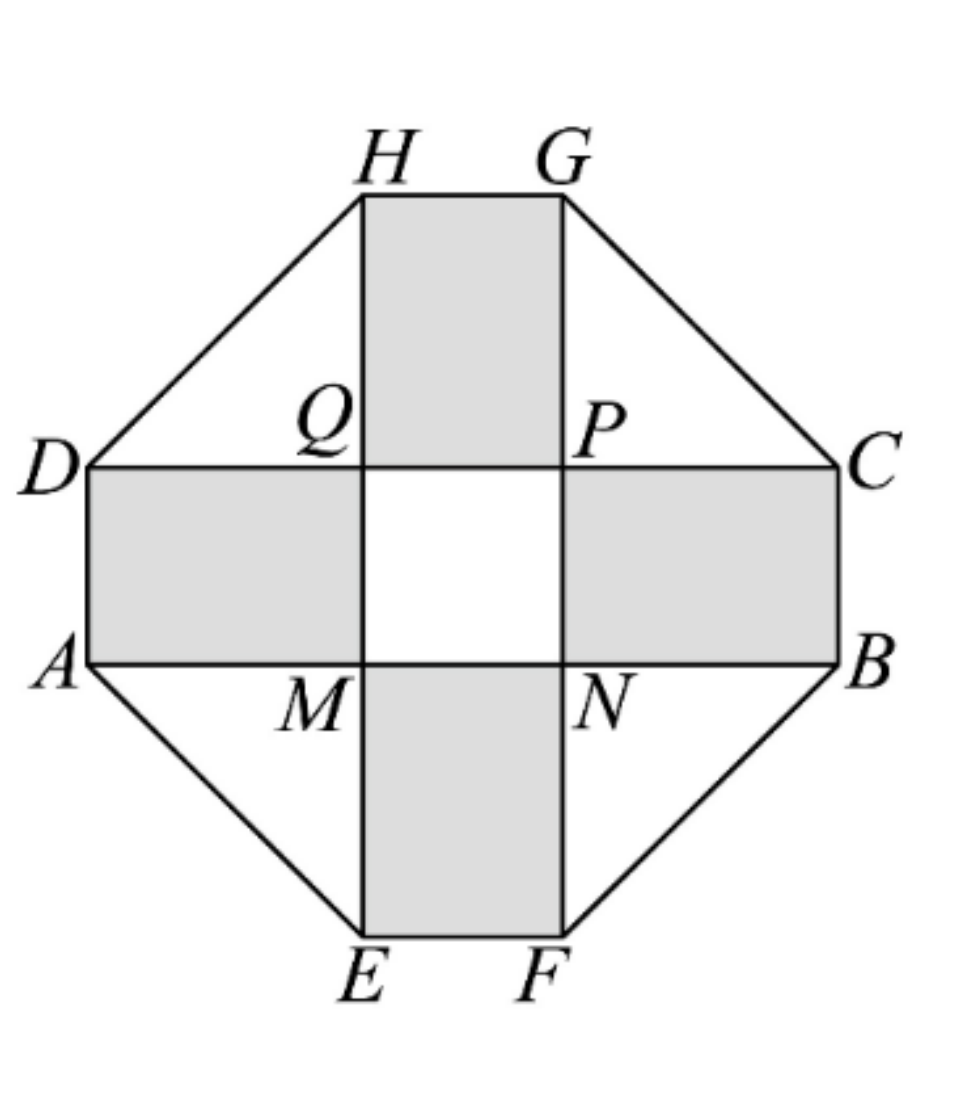
\includegraphics[width=0.34\textwidth]{figures/cross_octagon_h64.png}
\end{center}

\begin{enumerate}[label=(\arabic*)]
\item 设 $DQ$ 长为 $y\mathrm{m}$（$y>0$），用 $x$ 表示 $y$，并求出 $x$ 的取值范围；
\item 如何设计 $AD$ 可使总造价最低，并求出最低造价.
\item 若总造价 $W$ 不超过 69000 元，求 $AD$ 长 $x$ 的取值范围.
\end{enumerate}

\ifanswer
\solbegin
\stepm{(1)}{设 $DQ$ 长为 $y\mathrm{m}$，因为十字形区域面积为 $200\text{m}^2$，}
\step{所以 $4xy+x^2=200$，解得 $y=\dfrac{200-x^2}{4x}=\dfrac{50}{x}-\dfrac x4$；\dots\dots2 分}
\step{因为 $y>0$，所以 $x^2<200$，因为 $x>0$，所以 $0<x<10\sqrt2$.\dots\dots4 分}
\stepm{(2)}{四个矩形地砖面积 $S_{\text{四个矩形}}=4xy=200-x^2$，}
\step{造价 $W_{\text{四个矩形}}=105(200-x^2)$；}
\step{四个三角形草坪面积 $S_{\text{三角形}}=4\times\dfrac12y^2=2\left(\dfrac{50}{x}-\dfrac x4\right)^2=\dfrac{5000}{x^2}+\dfrac{x^2}8-50$，}
\step{造价 $W_{\text{三角形}}=40\left(\dfrac{5000}{x^2}+\dfrac{x^2}8-50\right)$；}
\step{正方形花坛面积 $S_{\text{正方形}}=x^2$，造价 $W_{\text{正方形}}=2100x^2$；}
\step{总造价 $W=W_{\text{四个矩形}}+W_{\text{三角形}}+W_{\text{正方形}}$}
\step{$=105(200-x^2)+40\left(\dfrac{5000}{x^2}+\dfrac{x^2}8-50\right)+2100x^2$，}
\step{化简得 $W=2000x^2+19000+\dfrac{200000}{x^2}$（$0<x<10\sqrt2$）.\dots\dots6 分}
\step{因为 $2000x^2+\dfrac{200000}{x^2}\geqslant40000$，}
\step{当且仅当 $x=\sqrt{10}$（在 $x$ 范围中）时取等号，此时 $W=59000$ 元.}
\step{综上，当 $AD$ 的长为 $\sqrt{10}$ 时，总造价最低，为 59000 元.\dots\dots8 分}
% 原卷 (3) 定义域印作 0<x<2√10，与 (1) 所得 0<x<10√2 不一致，照录（见文件头“原卷笔误”④）
\stepm{(3)}{由（2）得 $W=2000x^2+19000+\dfrac{200000}{x^2}$（$0<x<2\sqrt{10}$）.}
\step{总造价不超过 69000 元，即 $W=2000x^2+19000+\dfrac{200000}{x^2}\leqslant69000$，}
\step{化简得 $x^2+\dfrac{100}{x^2}\leqslant25$，\dots\dots10 分}
\step{即 $(x^2)^2-25x^2+100=(x^2-20)(x^2-5)\leqslant0$，即 $\sqrt5\leqslant x\leqslant2\sqrt5$，}
% 原卷末句“取值范围[√5,2√5]”脱“为”，照录（见文件头“原卷笔误”⑤）
\step{所以 $AD$ 长 $x$ 的取值范围$[\sqrt5,2\sqrt5]$.\dots\dots12 分}
\solend
\fi

\ansspace[10]

\item 设 $a,b,c$ 为实数，集合 $S=\{x\mid(x+a)(x^2+bx+c)=0,x\in\R\}$.

\begin{enumerate}[label=(\arabic*)]
\item 若 $a=1,b=3,c=2$，求集合 $S$；
\item 若 $S=\{-2\}$，求 $a,b,c$ 满足的条件；
\item 设 $T=\{x\mid(ax+1)(cx^2+bx+1)=0,x\in\R\}$，当 $ac\neq0$ 时，如果 $\dfrac12\in S$，$-2\in T$，且
集合 $S,T$ 均恰有两个元素，求三元数对 $(a,b,c)$.
\end{enumerate}

\ifanswer
\solbegin
\stepm{(1)}{若 $a=1,b=3,c=2$，}
\step{则方程 $(x+a)(x^2+bx+c)=0$ 为 $(x+1)(x^2+3x+2)=0$，}
\step{即 $(x+1)^2(x+2)=0$，解得 $x=-1$ 或 $x=-2$，所以 $S=\{-1,-2\}$；}
\stepm{(2)}{由题意得 $-a\in S$，因为 $S=\{-2\}$，所以 $-2$ 是方程 $x+a=0$ 的根，}
\step{即 $-2+a=0$，解得 $a=2$. 由 $S=\{-2\}$，集合 $S$ 有且仅有一个元素，}
\step{即方程 $(x+a)(x^2+bx+c)=0$ 有且仅有一个根，}
\stepm{①}{若 $-2$ 是方程 $x^2+bx+c=0$ 的根，}
\step{则 $\Delta=b^2-4c=0$，且 $-\dfrac b2=-2$，解得 $b=4,c=4$；}
\stepm{②}{若 $-2$ 不是方程 $x^2+bx+c=0$ 的根，则方程 $x^2+bx+c=0$ 无实数根，}
\step{则 $\Delta=b^2-4c<0$，}
\step{综上所述，$\begin{cases}a=2\\ b=4\\ c=4\end{cases}$ 或 $\begin{cases}a=2\\ b^2-4c<0\end{cases}$.}
\stepm{(3)}{$S=\{x\mid(x+a)(x^2+bx+c)=0,x\in\R\}$，}
\step{$T=\{x\mid(ax+1)(cx^2+bx+1)=0,x\in\R\}$，}
\step{由题意得 $a\neq0$ 且 $c\neq0$，则 $-a\in S,-\dfrac1a\in T$，}
\step{且方程 $x^2+bx+c=0$ 与 $cx^2+bx+1=0$ 有相同的判别式 $\Delta=b^2-4c$，}
\step{即两方程根的个数相同. 由集合 $S,T$ 均恰有两个元素，则 $\Delta=b^2-4c\geqslant0$.}
\step{$S=\{x\mid(x+a)(x^2+bx+c)=0,x\in\R\}$，}
\step{因为 $\dfrac12\in S$，所以 $\dfrac12$ 是方程 $x+a=0$ 或 $x^2+bx+c=0$ 的根.}
\step{$T=\{x\mid(ax+1)(cx^2+bx+1)=0,x\in\R\}$，}
\step{由 $-\dfrac1a\in T$，且 $-2\in T$，则 $-2$ 是方程 $ax+1=0$ 或 $cx^2+bx+1=0$ 的根.}
\stepm{①}{当 $a=-\dfrac12$ 时，$\dfrac12$ 是方程 $x+a=0$ 的根，$-a=\dfrac12\in S$，则 $-\dfrac1a=2\in T$，}
\step{又 $-2\in T$，则 $T=\{-2,2\}$，}
\step{由 $T=\left\{x\mid\left(-\dfrac12x+1\right)(cx^2+bx+1)=0,x\in\R\right\}$，}
% 原卷句末为句号，本稿原错作逗号
\step{则 $-2$ 是方程 $cx^2+bx+1=0$ 的根，则 $4c-2b+1=0$.}
\stepm{(i)}{若 $\Delta=b^2-4c=0$，联立 $\begin{cases}4c-2b+1=0\\ b^2-4c=0\end{cases}$ 解得 $b=1,c=\dfrac14$.}
\step{验证：当 $a=-\dfrac12,b=1,c=\dfrac14$ 时，}
\step{$S=\left\{x\mid\left(x-\dfrac12\right)\left(x^2+x+\dfrac14\right)=0,x\in\R\right\}=\left\{-\dfrac12,\dfrac12\right\}$，}
\step{$T=\left\{x\mid\left(-\dfrac12x+1\right)\left(\dfrac14x^2+x+1\right)=0,x\in\R\right\}=\{-2,2\}$，满足题意；}
\stepm{(ii)}{若 $\Delta=b^2-4c>0$，方程 $cx^2+bx+1=0$ 有两个不相等的实数根，}
\step{又 $T=\{-2,2\}$，则方程 $cx^2+bx+1=0$ 的两根必为 $-2$ 和 2.}
\step{由韦达定理得 $\begin{cases}-2+2=-\dfrac bc\\ -2\times2=\dfrac1c\end{cases}$，解得 $b=0,c=-\dfrac14$；}
\step{验证：当 $a=-\dfrac12,b=0,c=-\dfrac14$ 时，}
\step{$S=\left\{x\mid\left(x-\dfrac12\right)\left(x^2-\dfrac14\right)=0,x\in\R\right\}=\left\{-\dfrac12,\dfrac12\right\}$，}
\step{$T=\left\{x\mid\left(-\dfrac12x+1\right)\left(-\dfrac14x^2+1\right)=0,x\in\R\right\}=\{-2,2\}$，满足题意；}
\stepm{②}{当 $a=\dfrac12$ 时，$-\dfrac1a=-2$，即 $-2$ 是方程 $ax+1=0$ 的根，}
\step{则 $-a=-\dfrac12\in S$，又 $\dfrac12\in S$，则 $S=\left\{-\dfrac12,\dfrac12\right\}$，}
\step{$S=\{x\mid(x+a)(x^2+bx+c)=0,x\in\R\}$，}
\step{则 $\dfrac12$ 是方程 $x^2+bx+c=0$ 的根，则 $\dfrac14+\dfrac12b+c=0$，即 $4c+2b+1=0$；}
\stepm{(i)}{若 $\Delta=b^2-4c=0$，联立 $\begin{cases}4c+2b+1=0\\ b^2-4c=0\end{cases}$ 解得 $b=-1,c=\dfrac14$.}
\step{验证：当 $a=\dfrac12,b=-1,c=\dfrac14$ 时，}
\step{$S=\left\{x\mid\left(x+\dfrac12\right)\left(x^2-x+\dfrac14\right)=0,x\in\R\right\}=\left\{-\dfrac12,\dfrac12\right\}$，}
\step{$T=\left\{x\mid\left(\dfrac12x+1\right)\left(\dfrac14x^2-x+1\right)=0,x\in\R\right\}=\{-2,2\}$，满足题意；}
% 原卷作“有两不等的实数根”，本稿原脱“的”
\stepm{(ii)}{若 $\Delta=b^2-4c>0$，方程 $x^2+bx+c=0$ 有两不等的实数根，}
% 原卷句末为句号，本稿原错作逗号
\step{又 $S=\left\{-\dfrac12,\dfrac12\right\}$，则方程 $x^2+bx+c=0$ 的两根必为 $-\dfrac12$ 和 $\dfrac12$.}
\step{由韦达定理得 $\begin{cases}-\dfrac12+\dfrac12=-b\\ -\dfrac12\times\dfrac12=c\end{cases}$，解得 $b=0,c=-\dfrac14$；}
\step{验证：当 $a=\dfrac12,b=0,c=-\dfrac14$ 时，}
\step{$S=\left\{x\mid\left(x+\dfrac12\right)\left(x^2-\dfrac14\right)=0,x\in\R\right\}=\left\{-\dfrac12,\dfrac12\right\}$，}
\step{$T=\left\{x\mid\left(\dfrac12x+1\right)\left(-\dfrac14x^2+1\right)=0,x\in\R\right\}=\{-2,2\}$，满足题意；}
\stepm{③}{当 $a\neq-\dfrac12$ 且 $a\neq\dfrac12$ 时，则 $\dfrac12$ 不是方程 $x+a=0$ 的根，}
\step{$-2$ 也不是方程 $ax+1=0$ 的根.}
% 原卷此句单根而称“两实数根”，语病，照录（见文件头“原卷笔误”⑥）
\step{由 $\dfrac12\in S,-2\in T$，则 $\dfrac12$ 是方程 $x^2+bx+c=0$ 的两实数根，}
\step{且 $-2$ 是方程 $cx^2+bx+1=0$ 的根，则有 $\begin{cases}\dfrac14+\dfrac12b+c=0\\ 4c-2b+1=0\end{cases}$，}
\step{解得 $b=0,c=-\dfrac14$.}
\step{验证：当 $a\neq-\dfrac12$ 且 $a\neq\dfrac12,b=0,c=-\dfrac14$ 时，有 $-a\neq\dfrac12,-a\neq-\dfrac12$.}
\step{$S=\left\{x\mid(x+a)\left(x^2-\dfrac14\right)=0,x\in\R\right\}=\left\{-a,-\dfrac12,\dfrac12\right\}$ 有三个元素，}
\step{故不满足题意；}
\step{综上所述，满足题意的所有三元数对 $(a,b,c)$ 有}
\step{$\left(-\dfrac12,1,\dfrac14\right)$，$\left(-\dfrac12,0,-\dfrac14\right)$，$\left(\dfrac12,-1,\dfrac14\right)$，$\left(\dfrac12,0,-\dfrac14\right)$.}
\solend
\fi

\ansspace*[10]

\end{enumerate}

\end{document}
"
%
% 原始材料：微信公众号“魔都数学加油站”文章，作者破晓，连载“27学年高一64”；
% 原文标题“27学年高一64——2026-2027年上海市格致中学高一上10月月考”；
% 原文链接：https://mp.weixin.qq.com/s/0DfB77nTJf7NdVI_FYXxeA。
% 页面标注发布时间 2026-10-17 21:58（上海）。
% 本次转录只据 `原图/高一64_格致中学_10月月考/` 的 14 张 PNG 逐页读图。
% 正文为 14 张 PNG 页（`01..14.png`）：第 12、13、14 页 2560×3620，
% 第 01—11 页 4762×6735（**同一篇各页分辨率不同**），均按页序读取。
% 14 页全为试卷正文页（卷首标题在第 1 页页顶，卷末解答题第 18 题解析止于第 14 页），
% 无封面页、目录页、二维码或宣传页。粉色斜排“魔都数学加油站”为卷面水印，与公众号页脚一并未录入。
%
% 卷首标题：照卷面印作“2026--2027 年格致中学高一上 10 月月考”，年份区间按全稿惯例排 en dash。
% 原卷只有一行标题、无副标题。
%
% 篇幅与题号：原卷自第 3 题起编号（第 1、2 题不在本卷内）。填空题 3—10（8 题）、
% 选择题 11—14（4 题）、解答题 15—18（4 题），共 16 题。本稿沿用原节与原题号，
% 只改排为全稿统一的大节样式（原卷小节标题为“一、填空题”“二、选择题”“三、解答题”）。
%
% 讲评版：原卷每题下直接印【答案】或【解析】。**只印【答案】的 1 题**（第 5 题），
% 本稿只给 \ans{}；其余 15 题都印【解析】（按全稿口径这类题不另提 \ans{}——第 11、13、14 题
% 的结论写在解析末句（“故选 A”“故选 D”等），亦照录在解析内）。**另有 1 题答案印在题干括号内**——
% 第 12 题（“( B )”，该题无【答案】/【解析】段），本稿按 高一37 第 13 题成例把括号留空、
% 答案另提为 \ans{$B$}。
%
% 副标题：原卷未印副标题。本稿按“知识模块”口径标作“集合与常用逻辑用语、不等式”：
% 16 题中集合与常用逻辑用语 8 题（第 4、9、10、11、12、13、16、18 题），
% 不等式 8 题（含一元二次方程与韦达定理、基本不等式、二次不等式、恒成立、分式不等式：
% 第 3、5、6、7、8、14、15、17 题），两类均达三分之一，故并标。口径同 高一59、高一63。
%
% 与原卷的排版差异：
%   ① 原卷每题下直接印【答案】/【解析】，本稿按全稿惯例将答案与解析置于答案版，试卷版保持干净；
%   ② 原卷未印副标题，本稿按“知识模块”口径补出；
%   ③ 原卷填空横线约三四个字宽，本稿按全稿惯例统一排 \blankline[4.4em]；
%   ④ 原卷实数集排斜体 $R$（第 4、7、8、13、15、18 题）或粗体 $\mathbf{R}$（第 18 题题干与
%      解析共 6 处），整数集排斜体 $Z$（第 9、13 题）或粗体 $\mathbf{Z}$（第 9 题解析末两行），
%      有理数集排粗体 $\mathbf{Q}$（第 13 题选项 A），本稿按全稿惯例统一改用 $\R$、$\Z$、$\Q$
%      （记号归一，粗体／斜体不作区分）；空集记号原卷作 $\varnothing$，照录；
%   ⑤ 第 4 题的补集**原卷用上划线记号 $\bar B$**（题干 1 处、解析 4 处，共 5 处），
%      与全稿惯例的 $\complement_U B$ 不同，本稿照录原卷的 $\bar B$；
%   ⑥ 原卷用描述法时竖线排细竖“$|$”（如 $\{x\mid|x|\geqslant2024\}$ 一类），本稿按全稿惯例排 \mid；
%   ⑦ 第 15—18 题的子问原卷各自另起一行、以“（1）”“（2）”“（3）”标号，本稿按全稿惯例用
%      enumerate 的 (1)(2)(3)；解析中的子问标号一律用 \stepm{(1)}{…}；
%      第 18 题解析中分情形的①②③与分小目的 (i)(ii)，按全稿惯例作 \stepm{①}{…}、\stepm{(i)}{…}；
%   ⑧ 第 13 题解析的“A 选项：”“B 选项：”“C 选项：”“D 选项：”原卷排**加粗**（共 4 处），
%      同 高一63“法一：”成例，本稿排 \stepm{A 选项：}{…} 一类（加粗着色、不改黑色基调），
%      冒号照原卷排全角；
%   ⑨ 第 17 题解析带评分档，原卷在档与档之间排一串点线（“………2 分”），
%      本稿照录为“\dots\dots2 分”一类（同 高一54 成例），共 5 处；
%   ⑩ 选择题的作答括号原卷排半角“(　　)”（第 11、13、14 题括号内空白、第 12 题括号内印 B），
%      本稿按全稿惯例排 \mbox{（\quad）}；选项字母后的句点照原卷排“A.”“B.”；
%   ⑪ 每道解答题原卷未留作答空白，本稿按全稿惯例加 \ansspace（末题用 \ansspace*）；
%   ⑫ 第 17 题题干右侧的十字形八边形示意图，本稿按原卷截图裁出（`figures/cross_octagon_h64.png`，
%      原分辨率裁切，未放大、未用 TikZ 重绘），图内阴影与点名照原卷。
%
% 原卷笔误/存疑（均照录未改，正文对应处另有 % 注）：
%   ① 第 8 题解析末两步自相矛盾：上一步已化为 $\dfrac x{x-1}<0$，下一步却印作
%      “即 $x(x+1)<0$，解得 $-1<x<0$”并给出解集 $(-1,0)$——由 $\dfrac x{x-1}<0$ 应得
%      $x(x-1)<0$、解集 $(0,1)$；已 8 倍放大确认原卷确为 $x+1$ 与 $(-1,0)$，照录未改。
%   ② 第 13 题 D 选项解析“乘法满足结合率”的“率”应为“律”（同段 A、B 选项均作“结合律”）。
%   ③ 第 13 题条件①“任意 $a,b\in G$. 有 $a*b\in G$；”在 $G$ 后印句号（其余三条均以逗号
%      接下文），疑为逗号之误，照录。
%   ④ 第 17 题 (3) 解析把定义域印作 $0<x<2\sqrt{10}$，与 (1) 所得 $0<x<10\sqrt2$ 不一致
%      （疑为 $10\sqrt2$ 之误）；照录未改。
%   ⑤ 第 17 题 (3) 末句“所以 $AD$ 长 $x$ 的取值范围$[\sqrt5,2\sqrt5]$.”脱一个“为”。
%   ⑥ 第 18 题 (3) ③“则 $\dfrac12$ 是方程 $x^2+bx+c=0$ 的**两**实数根”——只有一个数却称
%      “两实数根”，语病；照录。
%
% 插图：第 17 题题干有 1 幅十字形八边形示意图（原卷第 09 页右侧），已按原卷截图排入；
% 其余 13 页无任何图形、无“如图”字样（第 17 题的“图中”均指此图）。
%
\documentclass[a4paper,11pt]{article}
\usepackage{common}

\begin{document}

\examtitlest[3]{2026--2027 年格致中学高一上 10 月月考}{集合与常用逻辑用语、不等式}

\bigsec{一、填空题}

\begin{enumerate}
\setcounter{enumi}{2}

\item 已知一元二次方程 $x^2-nx+5=0$ 的两个实根分别为 $x_1$、$x_2$，且 $\dfrac1{x_1}+\dfrac1{x_2}=1$，则实数 $n$ 的值为\blankline[4.4em].

\ifanswer
\solbegin
\step{$\dfrac1{x_1}+\dfrac1{x_2}=\dfrac{x_1+x_2}{x_1x_2}=\dfrac n5=1$，所以 $n=5$.}
\solend
\fi

\item 全集为 $U=\R$，$A=\{x\mid|x|\geqslant2\}$，$B=\{y\mid y=x^2+1,x\in\R\}$，则 $A\cup\bar B=$\blankline[4.4em].

\ifanswer
\solbegin
\step{由题意得集合 $A=\{x\mid x\geqslant2\text{ 或 }x\leqslant-2\}$，}
\step{因为 $x^2+1\geqslant1$，所以集合 $B=\{x\mid x\geqslant1\}$，所以 $\bar B=\{x\mid x<1\}$，}
\step{则 $A\cup\bar B=\{x\mid x\geqslant2\text{ 或 }x<1\}$.}
\solend
\fi

\item 若 $x>2$，则 $4x+\dfrac1{x-2}$ 的最小值为\blankline[4.4em].

\ifanswer
\ans{$12$}
\fi

\item 已知关于 $x$ 不等式组$\begin{cases}(3x-2)(2x+3)\leqslant0\\ x-a<0\end{cases}$\!没有实数解，则实数 $a$ 的取值范围为\blankline[4.4em].

\ifanswer
\solbegin
\step{由题意得 $\begin{cases}-\dfrac32\leqslant x\leqslant\dfrac23\\ x<a\end{cases}$ 无解，所以 $a\leqslant-\dfrac32$.}
\solend
\fi

\item 若不等式 $\dfrac{x^2-8x+20}{mx^2-mx-1}<0$ 对一切 $x\in\R$ 都成立，则实数 $m$ 的取值范围为\blankline[4.4em].

\ifanswer
\solbegin
\step{因为 $x^2-8x+20=(x-4)^2+4\geqslant4>0$，所以 $mx^2-mx-1<0$，}
\step{当 $m=0$ 时，$mx^2-mx-1=-1<0$，不等式成立；}
\step{设 $y=mx^2-mx-1$，当 $m\neq0$ 时函数 $y$ 为二次函数，$y$ 要恒小于 0，}
\step{抛物线开口向下且与 $x$ 轴没有交点，即 $m<0$ 且 $\Delta<0$，得 $-4<m\leqslant0$，}
\step{故实数 $m$ 的取值范围为 $(-4,0]$.}
\solend
\fi

\item 已知关于 $x$ 的不等式 $\dfrac{ax-1}{x+b}>0$ 的解集为 $\{x\mid-1<x<2\}$，其中 $a$、$b\in\R$，则关于 $x$ 的不等式 $\dfrac{bx+1}{ax+1}<1$ 的解集为\blankline[4.4em].

\ifanswer
\solbegin
\step{不等式 $\dfrac{ax-1}{x+b}>0$ 等价于 $(ax-1)(x+b)>0$，即 $ax^2+(ab-1)x-b>0$，}
\step{所以 $-1$ 和 2 为方程 $ax^2+(ab-1)x-b=0$ 的两根，且 $a<0$，}
\step{由韦达定理得 $\begin{cases}-1+2=-\dfrac{ab-1}a\\ -1\times2=-\dfrac ba\end{cases}$，解得 $\begin{cases}a=-1\\ b=-2\end{cases}$，}
\step{所以原不等式为 $\dfrac{-2x+1}{-x+1}<1\Rightarrow\dfrac{-2x+1}{-x+1}-1<0\Rightarrow\dfrac{-x}{-x+1}<0\Rightarrow\dfrac x{x-1}<0$，}
% 原卷下一步印作“即 x(x+1)<0，解得 -1<x<0”，与上一步 x/(x-1)<0 不等价，
% 照录未改（见文件头“原卷笔误”①）
\step{即 $x(x+1)<0$，解得 $-1<x<0$，即不等式 $\dfrac{bx+1}{ax+1}<1$ 的解集为 $(-1,0)$.}
\solend
\fi

\item 已知集合 $M=\{x\mid|x|\leqslant2024,x\in\Z\}$，集合 $P$ 是 $M$ 的三元子集，即 $P=\{a,b,c\}\subseteq M$，$P$~中元素 $a,b,c$ 满足 $\begin{cases}\dfrac1a+\dfrac1b=\dfrac2c\\ a+c=2b\end{cases}$，则符合要求的集合 $P$ 有\blankline[4.4em]个.

\ifanswer
\solbegin
\step{由 $a+c=2b$，则 $a=2b-c$，代入 $\dfrac1a+\dfrac1b=\dfrac2c$，即 $\dfrac1{2b-c}=\dfrac2c-\dfrac1b=\dfrac{2b-c}{bc}$，}
\step{整理得 $(2b-c)^2=bc$，展开得 $4b^2-5bc+c^2=0$，}
\step{解得 $b=\dfrac c4$ 或 $b=c$（由集合的互异性，舍去），代入 $a+c=2b$ 得 $a=-\dfrac c2$，}
\step{则 $P=\left\{-\dfrac c2,\dfrac c4,c\right\}\subseteq\{x\mid-2024\leqslant x\leqslant2024,x\in\Z\}$，所以 $c$ 为 4 的整数倍，}
\step{且不为 0，则共有 $\dfrac{2024}4\times2=1012$ 个.}
\solend
\fi

\item 已知正整数 $n\geqslant2$，对集合 $\{1,2,3,\cdots,n\}$ 及其每一个非空子集 $X$，记
$X=\{x_1,x_2,\cdots,x_k\}$，其中 $x_1>x_2>\cdots>x_k$，定义一个运算“交替和”
$S_X=x_1-x_2+x_3\cdots+(-1)^{k+1}x_k$. 例如：对于集合 $X=\{9,6,4,2,1\}$，
$S_X=9-6+4-2+1=6$. 则当 $n=7$ 时，集合 $\{1,2,3,\cdots,n\}$ 的所有子集的“交替和”的总
和为\blankline[4.4em].

\ifanswer
\solbegin
\step{由题意得集合 $\{7\}$ 的“交替和”为 7.}
\step{集合 $\{1,2,3,4,5,6,7\}$ 的所有 $2^7$ 个子集中，除去集合 $\{7\}$ 外，}
\step{还有 $2^7-2$ 个非空子集，这 $2^7-2$ 个非空子集中不含元素 7 的集合，}
\step{即 $\{1,2,3,4,5,6\}$ 的非空子集，共有 $2^6-1$ 个，设为 $A_i(i=1,2,\cdots,2^6-1)$；}
\step{则这 $2^7-2$ 个非空子集中含元素 7 的集合，也共有 $2^6-1$ 个，}
\step{这样的集合都可以看成相应地在每个不含 7 的集合中再加上元素 7 得到，}
\step{即 $A_i\cup\{7\}$.}
\step{对 $A_i(i=1,2,\cdots,2^6-1)$ 中的任意集合 $A$，记 $A=\{x_1,x_2,\cdots,x_k\}$，}
\step{则“交替和”$S_A=x_1-x_2+x_3\cdots+(-1)^{k+1}x_k$，其中 $x_1>x_2>\cdots>x_k$，}
\step{由 $7>x_1>x_2>\cdots>x_k$，}
\step{则集合 $A\cup\{7\}$ 的“交替和”为 $7-[x_1-x_2+x_3\cdots+(-1)^{k+1}x_k]$，}
\step{则集合 $A$ 与集合 $A\cup\{7\}$ 的“交替和”之和为 7，下面举例说明：}
\step{如集合 $\{6,5,4,3,2,1\}$ 与集合 $\{7,6,5,4,3,2,1\}$，}
\step{$\{6,5,4,3,2,1\}$ 的“交替和”为 $6-5+4-3+2-1=3$，}
% 原卷此句在页末折为两个印刷行（“……的“交替和”为”／“7-6+5-4+3-2+1=……”），
% 本稿原并作一条，现照原卷拆开（原卷原样两行 / 本稿原错处：并作一行）
\step{$\{7,6,5,4,3,2,1\}$ 的“交替和”为}
\step{$7-6+5-4+3-2+1=7-(6-5+4-3+2-1)=7-3$，}
\step{即集合 $\{6,5,4,3,2,1\}$ 与集合 $\{7,6,5,4,3,2,1\}$ 的“交替和”之和为 7.}
\step{综上，把这 $2^7-2$ 个非空子集两两结组后分别计算每一组中“交替和”之和，}
\step{且每组中“交替和”之和都为 7，共有 $2^6-1$ 组.}
\step{故集合 $\{1,2,3,4,5,6,7\}$ 所有“交替和”之和，}
\step{由各组之和再加集合 $\{7\}$ 的“交替和”7 即可，}
\step{综上所述，当 $n=7$ 时，集合 $\{1,2,3,\cdots,n\}$ 的所有子集的所有“交替和”之和}
\step{为 $7\times(2^6-1)+7=448$.}
\solend
\fi

\end{enumerate}

\bigsec{二、选择题}

\begin{enumerate}
\setcounter{enumi}{10}

\item 若 $a$、$b\in\R$，则“$a<b<0$”是“$a^2>b^2$”的\mbox{（\quad）}条件.

\keepwithprev
A. 充分非必要\qquad B. 必要非充分

C. 充要\qquad D. 既非充分也非必要

\ifanswer
\solbegin
\step{由 $a<b<0\Rightarrow-a>-b>0\Rightarrow(-a)^2>(-b)^2\Rightarrow a^2>b^2$，}
\step{因此由 $a<b<0$ 可以推出 $a^2>b^2$，}
\step{但是当 $a=1$，$b=0$ 时，显然 $a^2>b^2$ 成立，但是 $a<b<0$ 不成立，}
\step{因此由 $a^2>b^2$ 不一定能推出 $a<b<0$，}
\step{因此“$a<b<0$”是“$a^2>b^2$”的充分非必要条件. 故选 $A$.}
\solend
\fi

% 第 12 题答案“B”直接印在题干括号内“(  B  )”，且该题无【答案】/【解析】段；
% 按 高一37 第 13 题的成例括号留空、答案另提为 \ans{}（见文件头）
\item 用反证法证明结论“$a$、$b$、$c$ 至少有一个是正数”时，应假设\mbox{（\quad）}

\keepwithprev
A. $a$、$b$、$c$ 都是正数\qquad B. $a$、$b$、$c$ 都不是正数

C. $a$、$b$、$c$ 至多有一个正数\qquad D. $a$、$b$、$c$ 至多有两个正数

\ifanswer
\ans{$B$}
\fi

\item “群”的概念由数学家伽罗瓦在 19 世纪 30 年代开创，群论虽起源于对代数多项式方程
的研究，但在量子力学、晶体结构学等其他学科中也有十分广泛的应用.“群”的定义是：

设 $G$ 为某种元素组成的一个非空集合，若在 $G$ 内定义一个运算“*”，满足以下条件：

% 原卷条件①在 G 后印句号，疑为逗号之误，照录（见文件头“原卷笔误”③）
①任意 $a,b\in G$. 有 $a*b\in G$；

②如 $a,b,c\in G$，有 $(a*b)*c=a*(b*c)$；

③在 $G$ 中有一个元素 $e$，对任意 $a\in G$，都有 $a*e=e*a=a$，称 $e$ 为 $G$ 的单位元；

④任意 $a\in G$，在 $G$ 中存在唯一确定的 $b$，使 $a*b=b*a=e$，称 $b$ 为 $a$ 的逆元；

此时称 $(G,*)$ 为一个群.

例如实数集 $\R$ 和实数集上的加法运算“+”就构成一个群 $(\R,+)$，其单位元是 0，每一个数
的逆元是其相反数，那么下列说法中，错误的是\mbox{（\quad）}

\keepwithprev
A. $G=\Q$，则 $(G,+)$ 为一个群

B. $G=\{\sqrt2m+\sqrt3n\mid m,n\in\Z\}$，$(G,+)$ 为一个群

C. $G=\{-1,1\}$，则 $(G,\times)$ 为一个群

D. $G=\{x\mid x=2k+1,k\in\Z\}$，则 $(G,\times)$ 为一个群

\ifanswer
\solbegin
\stepm{A 选项：}{有理数的和还是有理数，求和满足结合律，}
\step{设 $a\in\Q$，单位元为 $e$，则 $a+e=a$，故 $e=0$，}
\step{所以每一个数的相反数为其逆元，故 $(G,+)$ 为一个群，选项 A 正确；}
\stepm{B 选项：}{$G=\{\sqrt2m+\sqrt3n\mid m,n\in\Z\}$ 中的任何两个数相加还是属于}
\step{$G=\{\sqrt2m+\sqrt3n\mid m,n\in\Z\}$，求和满足结合律，}
\step{设 $\sqrt2x+\sqrt3y\in G,x,y\in\Z$，单位元为 $e$，}
\step{则 $\sqrt2x+\sqrt3y+e=\sqrt2x+\sqrt3y$，所以 $e=0$，}
\step{每一个数的相反数为其逆元，$(G,+)$ 为一个群，选项 B 正确；}
\stepm{C 选项：}{$G=\{-1,1\}$ 中的两个元素相乘，其积可能为 1 或 $-1$，又 $1\in G,-1\in G$，}
\step{设 $a\in G$，单位元为 $e$，则 $a\times e=a$，故 $e=1,1$ 的逆元为 $1,-1$ 的逆元为 $-1$，}
\step{所以 $(G,\times)$ 为一个群，选项 C 正确；}
% 原卷“乘法满足结合率”的“率”应为“律”（同段 A、B 选项均作“结合律”），照录（见文件头“原卷笔误”②）
\stepm{D 选项：}{两个奇数相乘还是奇数，乘法满足结合率，}
\step{设 $a\in G$，单位元为 $e$，则 $a\times e=a$，故 $e=1$，}
\step{又 $3\in G$，故存在 $b\in G$，使得 $3b=1$，则 $b=\dfrac13$，矛盾，}
\step{故 $(G,\times)$ 不为一个群，选项 D 错误.}
\step{故选 $D$.}
\solend
\fi

\item 已知 $a$、$b$、$c\in\R$，若关于 $x$ 的不等式 $0\leqslant x+\dfrac ax+b\leqslant\dfrac cx-1$ 的解集为 $[x_1,x_2]\cup\{x_3\}$
（$x_3>x_2>x_1>0$），则\mbox{（\quad）}

\keepwithprev
A. 不存在有序数组 $(a,b,c)$，使得 $x_2-x_1=1$

B. 存在唯一有序数组 $(a,b,c)$，使得 $x_2-x_1=1$

C. 有且只有两组有序数组 $(a,b,c)$，使得 $x_2-x_1=1$

D. 存在无穷多组有序数组 $(a,b,c)$，使得 $x_2-x_1=1$

\ifanswer
\solbegin
\step{因为不等式 $0\leqslant x+\dfrac ax+b\leqslant\dfrac cx-1$ 的解集为 $[x_1,x_2]\cup\{x_3\}$（$x_3>x_2>x_1>0$），}
\step{所以 $0\leqslant x^2+bx+a\leqslant c-x$ 在 $[x_1,x_2]\cup\{x_3\}$ 上成立，}
\step{假设 $x_1=m$，$x_2=m+1$，$x_3=n$，}
\step{则 $c-n=0=n^2+bn+a$，由 $x_3$ 为一个独立的数得出，}
\step{所以 $n=c$，且 $m+1$ 与 $n$ 为方程 $x^2+bx+a=0$ 的两个根，}
\step{因为 $x_3>x_2>x_1>0$，所以 $-b=m+n+1=m+c+1$，$a=mn+n=mc+c$，}
\step{所以 $b=-m-c-1$，}
\step{且点 $(x_1,x_1^2+bx_1+a)$ 为 $y=x^2+bx+a$ 与 $y=c-x$ 的左交点，}
\step{所以 $m^2+bm+a=c-m$ 且 $b=-m-c-1$，$a=mc+c$，}
\step{故 $m^2+bm+a=m^2-m^2-mc-m+mc+c=c-m$，所以 $c-m=c-m$ 恒成立，}
\step{所以不论 $a$、$b$、$c$ 取何值，$x_2-x_1=1$ 恒成立，}
\step{即存在无穷多组有序数组 $(a,b,c)$，使得 $x_2-x_1=1$，}
\step{故选项 $A$、$B$、$C$ 错误，选项 $D$ 正确. 故选 $D$.}
\solend
\fi

\end{enumerate}

\bigsec{三、解答题}

\begin{enumerate}
\setcounter{enumi}{14}

\item 已知函数 $f(x)=(a-1)x^2-ax+1$，$a\in\R$.

\begin{enumerate}[label=(\arabic*)]
\item 若不等式 $f(x)<0$ 的解集为 $\left(\dfrac13,1\right)$，求实数 $a$ 的值；
\item 当 $a>1$ 时，解关于 $x$ 的不等式 $f(x)\geqslant0$.
\end{enumerate}

\ifanswer
\solbegin
\stepm{(1)}{因为不等式 $f(x)<0$ 的解集为 $\left(\dfrac13,1\right)$，}
\step{所以不等式对应的方程 $(a-1)x^2-ax+1=0$ 的两根分别为 $\dfrac13$、1，}
\step{由根与系数的关系得 $\begin{cases}1+\dfrac13=\dfrac a{a-1}\\ 1\times\dfrac13=\dfrac1{a-1}\end{cases}$，解得 $a=4$；}
\stepm{(2)}{不等式 $(a-1)x^2-ax+1\geqslant0$（$a>1$）可化为 $(x-1)[(a-1)x-1]\geqslant0$，}
\step{不等式对应方程的两根为 $x_1=1$，$x_2=\dfrac1{a-1}$，}
\step{①当 $\dfrac1{a-1}=1$，即 $a=2$ 时，不等式为 $(x-1)^2\geqslant0$，解集为 $\R$；}
\step{②当 $\dfrac1{a-1}>1$，即 $1<a<2$ 时，解不等式得 $x\leqslant1$ 或 $x\geqslant\dfrac1{a-1}$；}
\step{③当 $\dfrac1{a-1}<1$，即 $a>2$ 时，解不等式得 $x\leqslant\dfrac1{a-1}$ 或 $x\geqslant1$；}
\step{综上，$a=2$ 时，不等式的解集为 $\R$，}
\step{$1<a<2$ 时，不等式的解集为 $(-\infty,1]\cup\left[\dfrac1{a-1},+\infty\right)$，}
\step{$a>2$ 时，不等式的解集为 $\left(-\infty,\dfrac1{a-1}\right]\cup[1,+\infty)$.}
\solend
\fi

\ansspace[6]

\item 若集合 $A=\{x\mid x^2+5x-6=0\}$，$B=\{x\mid x^2+2(m+1)x+m^2-3=0\}$.

\begin{enumerate}[label=(\arabic*)]
\item 若 $m=0$，写出 $A\cup B$ 的子集个数；
\item 若 $A\cap B=B$，求实数 $m$ 的取值范围.
\end{enumerate}

\ifanswer
\solbegin
\stepm{(1)}{当 $m=0$ 时，$B=\{1,-3\}$，}
\step{因为 $A=\{x\mid x^2+5x-6=0\}=\{-6,1\}$，}
\step{所以 $A\cup B=\{-6,-3,1\}$，集合元素个数为 3 个，}
\step{故 $A\cup B$ 的子集个数为 $2^3=8$.}
\stepm{(2)}{因为 $A\cap B=B$，所以 $B\subseteq A$，}
\step{$\Delta=4(m+1)^2-4(m^2-3)=8m+16$，}
\step{当 $\Delta<0$，即 $m<-2$ 时，$B=\varnothing$，符合题意，}
\step{当 $\Delta=0$，即 $m=-2$ 时，$B=\{1\}$，符合题意，}
\step{当 $\Delta>0$，即 $m>-2$ 时，若 $B\subseteq A$，则 $B=\{-6,1\}$，}
\step{即 $\begin{cases}-2(m+1)=-5\\ m^2-3=-6\end{cases}$，方程组无解，}
\step{综上所述，$m$ 的取值范围为 $(-\infty,-2]$.}
\solend
\fi

\ansspace[6]

\item 2025 年上海奇迹花园国际艺术花展于 9 月 20 日正式启幕，本次花展首次实现沉浸 IP
展、花卉景观、跨界艺术、光影夜花园四展合一，为市民游客打造一个可游、可赏、可感
的秋季治愈系童话世界. 某公园受此启发打算设计一个八边形活动区域，该区域的主体造
型平面图是由两个相同的矩形 $ABCD$ 和 $EFGH$ 构成的十字形地域，十字形的面积为
$200\text{m}^2$. 计划在正方形 $MNPQ$ 上建一座花坛，造价为 2100 元$/\text{m}^2$；在四个相同的矩形
（图中阴影部分）上铺地砖，造价为 105 元$/\text{m}^2$；再在四个空角（图中四个三角
形）上铺草坪，造价为 40 元$/\text{m}^2$. 设 $AD$ 长为 $x\mathrm{m}$（$x>0$），总造价为 $W$ 元，求：

\begin{center}
% 插图取自原卷第 09 页右侧截图（原分辨率裁切，未用 TikZ 重绘），阴影与点名照原卷
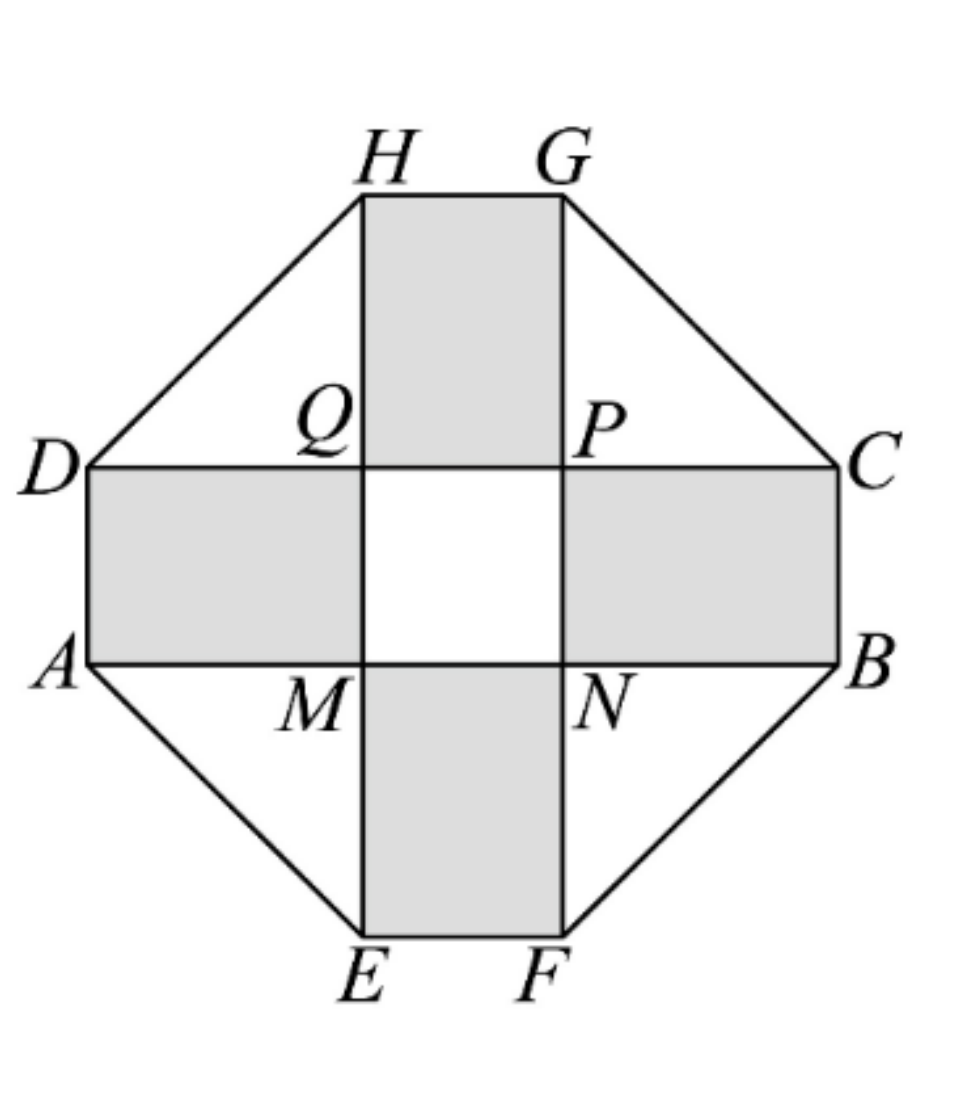
\includegraphics[width=0.34\textwidth]{figures/cross_octagon_h64.png}
\end{center}

\begin{enumerate}[label=(\arabic*)]
\item 设 $DQ$ 长为 $y\mathrm{m}$（$y>0$），用 $x$ 表示 $y$，并求出 $x$ 的取值范围；
\item 如何设计 $AD$ 可使总造价最低，并求出最低造价.
\item 若总造价 $W$ 不超过 69000 元，求 $AD$ 长 $x$ 的取值范围.
\end{enumerate}

\ifanswer
\solbegin
\stepm{(1)}{设 $DQ$ 长为 $y\mathrm{m}$，因为十字形区域面积为 $200\text{m}^2$，}
\step{所以 $4xy+x^2=200$，解得 $y=\dfrac{200-x^2}{4x}=\dfrac{50}{x}-\dfrac x4$；\dots\dots2 分}
\step{因为 $y>0$，所以 $x^2<200$，因为 $x>0$，所以 $0<x<10\sqrt2$.\dots\dots4 分}
\stepm{(2)}{四个矩形地砖面积 $S_{\text{四个矩形}}=4xy=200-x^2$，}
\step{造价 $W_{\text{四个矩形}}=105(200-x^2)$；}
\step{四个三角形草坪面积 $S_{\text{三角形}}=4\times\dfrac12y^2=2\left(\dfrac{50}{x}-\dfrac x4\right)^2=\dfrac{5000}{x^2}+\dfrac{x^2}8-50$，}
\step{造价 $W_{\text{三角形}}=40\left(\dfrac{5000}{x^2}+\dfrac{x^2}8-50\right)$；}
\step{正方形花坛面积 $S_{\text{正方形}}=x^2$，造价 $W_{\text{正方形}}=2100x^2$；}
\step{总造价 $W=W_{\text{四个矩形}}+W_{\text{三角形}}+W_{\text{正方形}}$}
\step{$=105(200-x^2)+40\left(\dfrac{5000}{x^2}+\dfrac{x^2}8-50\right)+2100x^2$，}
\step{化简得 $W=2000x^2+19000+\dfrac{200000}{x^2}$（$0<x<10\sqrt2$）.\dots\dots6 分}
\step{因为 $2000x^2+\dfrac{200000}{x^2}\geqslant40000$，}
\step{当且仅当 $x=\sqrt{10}$（在 $x$ 范围中）时取等号，此时 $W=59000$ 元.}
\step{综上，当 $AD$ 的长为 $\sqrt{10}$ 时，总造价最低，为 59000 元.\dots\dots8 分}
% 原卷 (3) 定义域印作 0<x<2√10，与 (1) 所得 0<x<10√2 不一致，照录（见文件头“原卷笔误”④）
\stepm{(3)}{由（2）得 $W=2000x^2+19000+\dfrac{200000}{x^2}$（$0<x<2\sqrt{10}$）.}
\step{总造价不超过 69000 元，即 $W=2000x^2+19000+\dfrac{200000}{x^2}\leqslant69000$，}
\step{化简得 $x^2+\dfrac{100}{x^2}\leqslant25$，\dots\dots10 分}
\step{即 $(x^2)^2-25x^2+100=(x^2-20)(x^2-5)\leqslant0$，即 $\sqrt5\leqslant x\leqslant2\sqrt5$，}
% 原卷末句“取值范围[√5,2√5]”脱“为”，照录（见文件头“原卷笔误”⑤）
\step{所以 $AD$ 长 $x$ 的取值范围$[\sqrt5,2\sqrt5]$.\dots\dots12 分}
\solend
\fi

\ansspace[10]

\item 设 $a,b,c$ 为实数，集合 $S=\{x\mid(x+a)(x^2+bx+c)=0,x\in\R\}$.

\begin{enumerate}[label=(\arabic*)]
\item 若 $a=1,b=3,c=2$，求集合 $S$；
\item 若 $S=\{-2\}$，求 $a,b,c$ 满足的条件；
\item 设 $T=\{x\mid(ax+1)(cx^2+bx+1)=0,x\in\R\}$，当 $ac\neq0$ 时，如果 $\dfrac12\in S$，$-2\in T$，且
集合 $S,T$ 均恰有两个元素，求三元数对 $(a,b,c)$.
\end{enumerate}

\ifanswer
\solbegin
\stepm{(1)}{若 $a=1,b=3,c=2$，}
\step{则方程 $(x+a)(x^2+bx+c)=0$ 为 $(x+1)(x^2+3x+2)=0$，}
\step{即 $(x+1)^2(x+2)=0$，解得 $x=-1$ 或 $x=-2$，所以 $S=\{-1,-2\}$；}
\stepm{(2)}{由题意得 $-a\in S$，因为 $S=\{-2\}$，所以 $-2$ 是方程 $x+a=0$ 的根，}
\step{即 $-2+a=0$，解得 $a=2$. 由 $S=\{-2\}$，集合 $S$ 有且仅有一个元素，}
\step{即方程 $(x+a)(x^2+bx+c)=0$ 有且仅有一个根，}
\stepm{①}{若 $-2$ 是方程 $x^2+bx+c=0$ 的根，}
\step{则 $\Delta=b^2-4c=0$，且 $-\dfrac b2=-2$，解得 $b=4,c=4$；}
\stepm{②}{若 $-2$ 不是方程 $x^2+bx+c=0$ 的根，则方程 $x^2+bx+c=0$ 无实数根，}
\step{则 $\Delta=b^2-4c<0$，}
\step{综上所述，$\begin{cases}a=2\\ b=4\\ c=4\end{cases}$ 或 $\begin{cases}a=2\\ b^2-4c<0\end{cases}$.}
\stepm{(3)}{$S=\{x\mid(x+a)(x^2+bx+c)=0,x\in\R\}$，}
\step{$T=\{x\mid(ax+1)(cx^2+bx+1)=0,x\in\R\}$，}
\step{由题意得 $a\neq0$ 且 $c\neq0$，则 $-a\in S,-\dfrac1a\in T$，}
\step{且方程 $x^2+bx+c=0$ 与 $cx^2+bx+1=0$ 有相同的判别式 $\Delta=b^2-4c$，}
\step{即两方程根的个数相同. 由集合 $S,T$ 均恰有两个元素，则 $\Delta=b^2-4c\geqslant0$.}
\step{$S=\{x\mid(x+a)(x^2+bx+c)=0,x\in\R\}$，}
\step{因为 $\dfrac12\in S$，所以 $\dfrac12$ 是方程 $x+a=0$ 或 $x^2+bx+c=0$ 的根.}
\step{$T=\{x\mid(ax+1)(cx^2+bx+1)=0,x\in\R\}$，}
\step{由 $-\dfrac1a\in T$，且 $-2\in T$，则 $-2$ 是方程 $ax+1=0$ 或 $cx^2+bx+1=0$ 的根.}
\stepm{①}{当 $a=-\dfrac12$ 时，$\dfrac12$ 是方程 $x+a=0$ 的根，$-a=\dfrac12\in S$，则 $-\dfrac1a=2\in T$，}
\step{又 $-2\in T$，则 $T=\{-2,2\}$，}
\step{由 $T=\left\{x\mid\left(-\dfrac12x+1\right)(cx^2+bx+1)=0,x\in\R\right\}$，}
% 原卷句末为句号，本稿原错作逗号
\step{则 $-2$ 是方程 $cx^2+bx+1=0$ 的根，则 $4c-2b+1=0$.}
\stepm{(i)}{若 $\Delta=b^2-4c=0$，联立 $\begin{cases}4c-2b+1=0\\ b^2-4c=0\end{cases}$ 解得 $b=1,c=\dfrac14$.}
\step{验证：当 $a=-\dfrac12,b=1,c=\dfrac14$ 时，}
\step{$S=\left\{x\mid\left(x-\dfrac12\right)\left(x^2+x+\dfrac14\right)=0,x\in\R\right\}=\left\{-\dfrac12,\dfrac12\right\}$，}
\step{$T=\left\{x\mid\left(-\dfrac12x+1\right)\left(\dfrac14x^2+x+1\right)=0,x\in\R\right\}=\{-2,2\}$，满足题意；}
\stepm{(ii)}{若 $\Delta=b^2-4c>0$，方程 $cx^2+bx+1=0$ 有两个不相等的实数根，}
\step{又 $T=\{-2,2\}$，则方程 $cx^2+bx+1=0$ 的两根必为 $-2$ 和 2.}
\step{由韦达定理得 $\begin{cases}-2+2=-\dfrac bc\\ -2\times2=\dfrac1c\end{cases}$，解得 $b=0,c=-\dfrac14$；}
\step{验证：当 $a=-\dfrac12,b=0,c=-\dfrac14$ 时，}
\step{$S=\left\{x\mid\left(x-\dfrac12\right)\left(x^2-\dfrac14\right)=0,x\in\R\right\}=\left\{-\dfrac12,\dfrac12\right\}$，}
\step{$T=\left\{x\mid\left(-\dfrac12x+1\right)\left(-\dfrac14x^2+1\right)=0,x\in\R\right\}=\{-2,2\}$，满足题意；}
\stepm{②}{当 $a=\dfrac12$ 时，$-\dfrac1a=-2$，即 $-2$ 是方程 $ax+1=0$ 的根，}
\step{则 $-a=-\dfrac12\in S$，又 $\dfrac12\in S$，则 $S=\left\{-\dfrac12,\dfrac12\right\}$，}
\step{$S=\{x\mid(x+a)(x^2+bx+c)=0,x\in\R\}$，}
\step{则 $\dfrac12$ 是方程 $x^2+bx+c=0$ 的根，则 $\dfrac14+\dfrac12b+c=0$，即 $4c+2b+1=0$；}
\stepm{(i)}{若 $\Delta=b^2-4c=0$，联立 $\begin{cases}4c+2b+1=0\\ b^2-4c=0\end{cases}$ 解得 $b=-1,c=\dfrac14$.}
\step{验证：当 $a=\dfrac12,b=-1,c=\dfrac14$ 时，}
\step{$S=\left\{x\mid\left(x+\dfrac12\right)\left(x^2-x+\dfrac14\right)=0,x\in\R\right\}=\left\{-\dfrac12,\dfrac12\right\}$，}
\step{$T=\left\{x\mid\left(\dfrac12x+1\right)\left(\dfrac14x^2-x+1\right)=0,x\in\R\right\}=\{-2,2\}$，满足题意；}
% 原卷作“有两不等的实数根”，本稿原脱“的”
\stepm{(ii)}{若 $\Delta=b^2-4c>0$，方程 $x^2+bx+c=0$ 有两不等的实数根，}
% 原卷句末为句号，本稿原错作逗号
\step{又 $S=\left\{-\dfrac12,\dfrac12\right\}$，则方程 $x^2+bx+c=0$ 的两根必为 $-\dfrac12$ 和 $\dfrac12$.}
\step{由韦达定理得 $\begin{cases}-\dfrac12+\dfrac12=-b\\ -\dfrac12\times\dfrac12=c\end{cases}$，解得 $b=0,c=-\dfrac14$；}
\step{验证：当 $a=\dfrac12,b=0,c=-\dfrac14$ 时，}
\step{$S=\left\{x\mid\left(x+\dfrac12\right)\left(x^2-\dfrac14\right)=0,x\in\R\right\}=\left\{-\dfrac12,\dfrac12\right\}$，}
\step{$T=\left\{x\mid\left(\dfrac12x+1\right)\left(-\dfrac14x^2+1\right)=0,x\in\R\right\}=\{-2,2\}$，满足题意；}
\stepm{③}{当 $a\neq-\dfrac12$ 且 $a\neq\dfrac12$ 时，则 $\dfrac12$ 不是方程 $x+a=0$ 的根，}
\step{$-2$ 也不是方程 $ax+1=0$ 的根.}
% 原卷此句单根而称“两实数根”，语病，照录（见文件头“原卷笔误”⑥）
\step{由 $\dfrac12\in S,-2\in T$，则 $\dfrac12$ 是方程 $x^2+bx+c=0$ 的两实数根，}
\step{且 $-2$ 是方程 $cx^2+bx+1=0$ 的根，则有 $\begin{cases}\dfrac14+\dfrac12b+c=0\\ 4c-2b+1=0\end{cases}$，}
\step{解得 $b=0,c=-\dfrac14$.}
\step{验证：当 $a\neq-\dfrac12$ 且 $a\neq\dfrac12,b=0,c=-\dfrac14$ 时，有 $-a\neq\dfrac12,-a\neq-\dfrac12$.}
\step{$S=\left\{x\mid(x+a)\left(x^2-\dfrac14\right)=0,x\in\R\right\}=\left\{-a,-\dfrac12,\dfrac12\right\}$ 有三个元素，}
\step{故不满足题意；}
\step{综上所述，满足题意的所有三元数对 $(a,b,c)$ 有}
\step{$\left(-\dfrac12,1,\dfrac14\right)$，$\left(-\dfrac12,0,-\dfrac14\right)$，$\left(\dfrac12,-1,\dfrac14\right)$，$\left(\dfrac12,0,-\dfrac14\right)$.}
\solend
\fi

\ansspace*[10]

\end{enumerate}

\end{document}
"
% 紧凑版：xelatex "\def\iscompact{1}% 高一64_格致中学_10月月考.tex
%   —— 高一上数学“2026-2027 年格致中学高一上 10 月月考”（讲评版）
% 试卷版：xelatex 高一64_格致中学_10月月考.tex
% 答案版：xelatex "\def\isanswer{1}% 高一64_格致中学_10月月考.tex
%   —— 高一上数学“2026-2027 年格致中学高一上 10 月月考”（讲评版）
% 试卷版：xelatex 高一64_格致中学_10月月考.tex
% 答案版：xelatex "\def\isanswer{1}\input{高一64_格致中学_10月月考.tex}"
% 紧凑版：xelatex "\def\iscompact{1}\input{高一64_格致中学_10月月考.tex}"
%
% 原始材料：微信公众号“魔都数学加油站”文章，作者破晓，连载“27学年高一64”；
% 原文标题“27学年高一64——2026-2027年上海市格致中学高一上10月月考”；
% 原文链接：https://mp.weixin.qq.com/s/0DfB77nTJf7NdVI_FYXxeA。
% 页面标注发布时间 2026-10-17 21:58（上海）。
% 本次转录只据 `原图/高一64_格致中学_10月月考/` 的 14 张 PNG 逐页读图。
% 正文为 14 张 PNG 页（`01..14.png`）：第 12、13、14 页 2560×3620，
% 第 01—11 页 4762×6735（**同一篇各页分辨率不同**），均按页序读取。
% 14 页全为试卷正文页（卷首标题在第 1 页页顶，卷末解答题第 18 题解析止于第 14 页），
% 无封面页、目录页、二维码或宣传页。粉色斜排“魔都数学加油站”为卷面水印，与公众号页脚一并未录入。
%
% 卷首标题：照卷面印作“2026--2027 年格致中学高一上 10 月月考”，年份区间按全稿惯例排 en dash。
% 原卷只有一行标题、无副标题。
%
% 篇幅与题号：原卷自第 3 题起编号（第 1、2 题不在本卷内）。填空题 3—10（8 题）、
% 选择题 11—14（4 题）、解答题 15—18（4 题），共 16 题。本稿沿用原节与原题号，
% 只改排为全稿统一的大节样式（原卷小节标题为“一、填空题”“二、选择题”“三、解答题”）。
%
% 讲评版：原卷每题下直接印【答案】或【解析】。**只印【答案】的 1 题**（第 5 题），
% 本稿只给 \ans{}；其余 15 题都印【解析】（按全稿口径这类题不另提 \ans{}——第 11、13、14 题
% 的结论写在解析末句（“故选 A”“故选 D”等），亦照录在解析内）。**另有 1 题答案印在题干括号内**——
% 第 12 题（“( B )”，该题无【答案】/【解析】段），本稿按 高一37 第 13 题成例把括号留空、
% 答案另提为 \ans{$B$}。
%
% 副标题：原卷未印副标题。本稿按“知识模块”口径标作“集合与常用逻辑用语、不等式”：
% 16 题中集合与常用逻辑用语 8 题（第 4、9、10、11、12、13、16、18 题），
% 不等式 8 题（含一元二次方程与韦达定理、基本不等式、二次不等式、恒成立、分式不等式：
% 第 3、5、6、7、8、14、15、17 题），两类均达三分之一，故并标。口径同 高一59、高一63。
%
% 与原卷的排版差异：
%   ① 原卷每题下直接印【答案】/【解析】，本稿按全稿惯例将答案与解析置于答案版，试卷版保持干净；
%   ② 原卷未印副标题，本稿按“知识模块”口径补出；
%   ③ 原卷填空横线约三四个字宽，本稿按全稿惯例统一排 \blankline[4.4em]；
%   ④ 原卷实数集排斜体 $R$（第 4、7、8、13、15、18 题）或粗体 $\mathbf{R}$（第 18 题题干与
%      解析共 6 处），整数集排斜体 $Z$（第 9、13 题）或粗体 $\mathbf{Z}$（第 9 题解析末两行），
%      有理数集排粗体 $\mathbf{Q}$（第 13 题选项 A），本稿按全稿惯例统一改用 $\R$、$\Z$、$\Q$
%      （记号归一，粗体／斜体不作区分）；空集记号原卷作 $\varnothing$，照录；
%   ⑤ 第 4 题的补集**原卷用上划线记号 $\bar B$**（题干 1 处、解析 4 处，共 5 处），
%      与全稿惯例的 $\complement_U B$ 不同，本稿照录原卷的 $\bar B$；
%   ⑥ 原卷用描述法时竖线排细竖“$|$”（如 $\{x\mid|x|\geqslant2024\}$ 一类），本稿按全稿惯例排 \mid；
%   ⑦ 第 15—18 题的子问原卷各自另起一行、以“（1）”“（2）”“（3）”标号，本稿按全稿惯例用
%      enumerate 的 (1)(2)(3)；解析中的子问标号一律用 \stepm{(1)}{…}；
%      第 18 题解析中分情形的①②③与分小目的 (i)(ii)，按全稿惯例作 \stepm{①}{…}、\stepm{(i)}{…}；
%   ⑧ 第 13 题解析的“A 选项：”“B 选项：”“C 选项：”“D 选项：”原卷排**加粗**（共 4 处），
%      同 高一63“法一：”成例，本稿排 \stepm{A 选项：}{…} 一类（加粗着色、不改黑色基调），
%      冒号照原卷排全角；
%   ⑨ 第 17 题解析带评分档，原卷在档与档之间排一串点线（“………2 分”），
%      本稿照录为“\dots\dots2 分”一类（同 高一54 成例），共 5 处；
%   ⑩ 选择题的作答括号原卷排半角“(　　)”（第 11、13、14 题括号内空白、第 12 题括号内印 B），
%      本稿按全稿惯例排 \mbox{（\quad）}；选项字母后的句点照原卷排“A.”“B.”；
%   ⑪ 每道解答题原卷未留作答空白，本稿按全稿惯例加 \ansspace（末题用 \ansspace*）；
%   ⑫ 第 17 题题干右侧的十字形八边形示意图，本稿按原卷截图裁出（`figures/cross_octagon_h64.png`，
%      原分辨率裁切，未放大、未用 TikZ 重绘），图内阴影与点名照原卷。
%
% 原卷笔误/存疑（均照录未改，正文对应处另有 % 注）：
%   ① 第 8 题解析末两步自相矛盾：上一步已化为 $\dfrac x{x-1}<0$，下一步却印作
%      “即 $x(x+1)<0$，解得 $-1<x<0$”并给出解集 $(-1,0)$——由 $\dfrac x{x-1}<0$ 应得
%      $x(x-1)<0$、解集 $(0,1)$；已 8 倍放大确认原卷确为 $x+1$ 与 $(-1,0)$，照录未改。
%   ② 第 13 题 D 选项解析“乘法满足结合率”的“率”应为“律”（同段 A、B 选项均作“结合律”）。
%   ③ 第 13 题条件①“任意 $a,b\in G$. 有 $a*b\in G$；”在 $G$ 后印句号（其余三条均以逗号
%      接下文），疑为逗号之误，照录。
%   ④ 第 17 题 (3) 解析把定义域印作 $0<x<2\sqrt{10}$，与 (1) 所得 $0<x<10\sqrt2$ 不一致
%      （疑为 $10\sqrt2$ 之误）；照录未改。
%   ⑤ 第 17 题 (3) 末句“所以 $AD$ 长 $x$ 的取值范围$[\sqrt5,2\sqrt5]$.”脱一个“为”。
%   ⑥ 第 18 题 (3) ③“则 $\dfrac12$ 是方程 $x^2+bx+c=0$ 的**两**实数根”——只有一个数却称
%      “两实数根”，语病；照录。
%
% 插图：第 17 题题干有 1 幅十字形八边形示意图（原卷第 09 页右侧），已按原卷截图排入；
% 其余 13 页无任何图形、无“如图”字样（第 17 题的“图中”均指此图）。
%
\documentclass[a4paper,11pt]{article}
\usepackage{common}

\begin{document}

\examtitlest[3]{2026--2027 年格致中学高一上 10 月月考}{集合与常用逻辑用语、不等式}

\bigsec{一、填空题}

\begin{enumerate}
\setcounter{enumi}{2}

\item 已知一元二次方程 $x^2-nx+5=0$ 的两个实根分别为 $x_1$、$x_2$，且 $\dfrac1{x_1}+\dfrac1{x_2}=1$，则实数 $n$ 的值为\blankline[4.4em].

\ifanswer
\solbegin
\step{$\dfrac1{x_1}+\dfrac1{x_2}=\dfrac{x_1+x_2}{x_1x_2}=\dfrac n5=1$，所以 $n=5$.}
\solend
\fi

\item 全集为 $U=\R$，$A=\{x\mid|x|\geqslant2\}$，$B=\{y\mid y=x^2+1,x\in\R\}$，则 $A\cup\bar B=$\blankline[4.4em].

\ifanswer
\solbegin
\step{由题意得集合 $A=\{x\mid x\geqslant2\text{ 或 }x\leqslant-2\}$，}
\step{因为 $x^2+1\geqslant1$，所以集合 $B=\{x\mid x\geqslant1\}$，所以 $\bar B=\{x\mid x<1\}$，}
\step{则 $A\cup\bar B=\{x\mid x\geqslant2\text{ 或 }x<1\}$.}
\solend
\fi

\item 若 $x>2$，则 $4x+\dfrac1{x-2}$ 的最小值为\blankline[4.4em].

\ifanswer
\ans{$12$}
\fi

\item 已知关于 $x$ 不等式组$\begin{cases}(3x-2)(2x+3)\leqslant0\\ x-a<0\end{cases}$\!没有实数解，则实数 $a$ 的取值范围为\blankline[4.4em].

\ifanswer
\solbegin
\step{由题意得 $\begin{cases}-\dfrac32\leqslant x\leqslant\dfrac23\\ x<a\end{cases}$ 无解，所以 $a\leqslant-\dfrac32$.}
\solend
\fi

\item 若不等式 $\dfrac{x^2-8x+20}{mx^2-mx-1}<0$ 对一切 $x\in\R$ 都成立，则实数 $m$ 的取值范围为\blankline[4.4em].

\ifanswer
\solbegin
\step{因为 $x^2-8x+20=(x-4)^2+4\geqslant4>0$，所以 $mx^2-mx-1<0$，}
\step{当 $m=0$ 时，$mx^2-mx-1=-1<0$，不等式成立；}
\step{设 $y=mx^2-mx-1$，当 $m\neq0$ 时函数 $y$ 为二次函数，$y$ 要恒小于 0，}
\step{抛物线开口向下且与 $x$ 轴没有交点，即 $m<0$ 且 $\Delta<0$，得 $-4<m\leqslant0$，}
\step{故实数 $m$ 的取值范围为 $(-4,0]$.}
\solend
\fi

\item 已知关于 $x$ 的不等式 $\dfrac{ax-1}{x+b}>0$ 的解集为 $\{x\mid-1<x<2\}$，其中 $a$、$b\in\R$，则关于 $x$ 的不等式 $\dfrac{bx+1}{ax+1}<1$ 的解集为\blankline[4.4em].

\ifanswer
\solbegin
\step{不等式 $\dfrac{ax-1}{x+b}>0$ 等价于 $(ax-1)(x+b)>0$，即 $ax^2+(ab-1)x-b>0$，}
\step{所以 $-1$ 和 2 为方程 $ax^2+(ab-1)x-b=0$ 的两根，且 $a<0$，}
\step{由韦达定理得 $\begin{cases}-1+2=-\dfrac{ab-1}a\\ -1\times2=-\dfrac ba\end{cases}$，解得 $\begin{cases}a=-1\\ b=-2\end{cases}$，}
\step{所以原不等式为 $\dfrac{-2x+1}{-x+1}<1\Rightarrow\dfrac{-2x+1}{-x+1}-1<0\Rightarrow\dfrac{-x}{-x+1}<0\Rightarrow\dfrac x{x-1}<0$，}
% 原卷下一步印作“即 x(x+1)<0，解得 -1<x<0”，与上一步 x/(x-1)<0 不等价，
% 照录未改（见文件头“原卷笔误”①）
\step{即 $x(x+1)<0$，解得 $-1<x<0$，即不等式 $\dfrac{bx+1}{ax+1}<1$ 的解集为 $(-1,0)$.}
\solend
\fi

\item 已知集合 $M=\{x\mid|x|\leqslant2024,x\in\Z\}$，集合 $P$ 是 $M$ 的三元子集，即 $P=\{a,b,c\}\subseteq M$，$P$~中元素 $a,b,c$ 满足 $\begin{cases}\dfrac1a+\dfrac1b=\dfrac2c\\ a+c=2b\end{cases}$，则符合要求的集合 $P$ 有\blankline[4.4em]个.

\ifanswer
\solbegin
\step{由 $a+c=2b$，则 $a=2b-c$，代入 $\dfrac1a+\dfrac1b=\dfrac2c$，即 $\dfrac1{2b-c}=\dfrac2c-\dfrac1b=\dfrac{2b-c}{bc}$，}
\step{整理得 $(2b-c)^2=bc$，展开得 $4b^2-5bc+c^2=0$，}
\step{解得 $b=\dfrac c4$ 或 $b=c$（由集合的互异性，舍去），代入 $a+c=2b$ 得 $a=-\dfrac c2$，}
\step{则 $P=\left\{-\dfrac c2,\dfrac c4,c\right\}\subseteq\{x\mid-2024\leqslant x\leqslant2024,x\in\Z\}$，所以 $c$ 为 4 的整数倍，}
\step{且不为 0，则共有 $\dfrac{2024}4\times2=1012$ 个.}
\solend
\fi

\item 已知正整数 $n\geqslant2$，对集合 $\{1,2,3,\cdots,n\}$ 及其每一个非空子集 $X$，记
$X=\{x_1,x_2,\cdots,x_k\}$，其中 $x_1>x_2>\cdots>x_k$，定义一个运算“交替和”
$S_X=x_1-x_2+x_3\cdots+(-1)^{k+1}x_k$. 例如：对于集合 $X=\{9,6,4,2,1\}$，
$S_X=9-6+4-2+1=6$. 则当 $n=7$ 时，集合 $\{1,2,3,\cdots,n\}$ 的所有子集的“交替和”的总
和为\blankline[4.4em].

\ifanswer
\solbegin
\step{由题意得集合 $\{7\}$ 的“交替和”为 7.}
\step{集合 $\{1,2,3,4,5,6,7\}$ 的所有 $2^7$ 个子集中，除去集合 $\{7\}$ 外，}
\step{还有 $2^7-2$ 个非空子集，这 $2^7-2$ 个非空子集中不含元素 7 的集合，}
\step{即 $\{1,2,3,4,5,6\}$ 的非空子集，共有 $2^6-1$ 个，设为 $A_i(i=1,2,\cdots,2^6-1)$；}
\step{则这 $2^7-2$ 个非空子集中含元素 7 的集合，也共有 $2^6-1$ 个，}
\step{这样的集合都可以看成相应地在每个不含 7 的集合中再加上元素 7 得到，}
\step{即 $A_i\cup\{7\}$.}
\step{对 $A_i(i=1,2,\cdots,2^6-1)$ 中的任意集合 $A$，记 $A=\{x_1,x_2,\cdots,x_k\}$，}
\step{则“交替和”$S_A=x_1-x_2+x_3\cdots+(-1)^{k+1}x_k$，其中 $x_1>x_2>\cdots>x_k$，}
\step{由 $7>x_1>x_2>\cdots>x_k$，}
\step{则集合 $A\cup\{7\}$ 的“交替和”为 $7-[x_1-x_2+x_3\cdots+(-1)^{k+1}x_k]$，}
\step{则集合 $A$ 与集合 $A\cup\{7\}$ 的“交替和”之和为 7，下面举例说明：}
\step{如集合 $\{6,5,4,3,2,1\}$ 与集合 $\{7,6,5,4,3,2,1\}$，}
\step{$\{6,5,4,3,2,1\}$ 的“交替和”为 $6-5+4-3+2-1=3$，}
% 原卷此句在页末折为两个印刷行（“……的“交替和”为”／“7-6+5-4+3-2+1=……”），
% 本稿原并作一条，现照原卷拆开（原卷原样两行 / 本稿原错处：并作一行）
\step{$\{7,6,5,4,3,2,1\}$ 的“交替和”为}
\step{$7-6+5-4+3-2+1=7-(6-5+4-3+2-1)=7-3$，}
\step{即集合 $\{6,5,4,3,2,1\}$ 与集合 $\{7,6,5,4,3,2,1\}$ 的“交替和”之和为 7.}
\step{综上，把这 $2^7-2$ 个非空子集两两结组后分别计算每一组中“交替和”之和，}
\step{且每组中“交替和”之和都为 7，共有 $2^6-1$ 组.}
\step{故集合 $\{1,2,3,4,5,6,7\}$ 所有“交替和”之和，}
\step{由各组之和再加集合 $\{7\}$ 的“交替和”7 即可，}
\step{综上所述，当 $n=7$ 时，集合 $\{1,2,3,\cdots,n\}$ 的所有子集的所有“交替和”之和}
\step{为 $7\times(2^6-1)+7=448$.}
\solend
\fi

\end{enumerate}

\bigsec{二、选择题}

\begin{enumerate}
\setcounter{enumi}{10}

\item 若 $a$、$b\in\R$，则“$a<b<0$”是“$a^2>b^2$”的\mbox{（\quad）}条件.

\keepwithprev
A. 充分非必要\qquad B. 必要非充分

C. 充要\qquad D. 既非充分也非必要

\ifanswer
\solbegin
\step{由 $a<b<0\Rightarrow-a>-b>0\Rightarrow(-a)^2>(-b)^2\Rightarrow a^2>b^2$，}
\step{因此由 $a<b<0$ 可以推出 $a^2>b^2$，}
\step{但是当 $a=1$，$b=0$ 时，显然 $a^2>b^2$ 成立，但是 $a<b<0$ 不成立，}
\step{因此由 $a^2>b^2$ 不一定能推出 $a<b<0$，}
\step{因此“$a<b<0$”是“$a^2>b^2$”的充分非必要条件. 故选 $A$.}
\solend
\fi

% 第 12 题答案“B”直接印在题干括号内“(  B  )”，且该题无【答案】/【解析】段；
% 按 高一37 第 13 题的成例括号留空、答案另提为 \ans{}（见文件头）
\item 用反证法证明结论“$a$、$b$、$c$ 至少有一个是正数”时，应假设\mbox{（\quad）}

\keepwithprev
A. $a$、$b$、$c$ 都是正数\qquad B. $a$、$b$、$c$ 都不是正数

C. $a$、$b$、$c$ 至多有一个正数\qquad D. $a$、$b$、$c$ 至多有两个正数

\ifanswer
\ans{$B$}
\fi

\item “群”的概念由数学家伽罗瓦在 19 世纪 30 年代开创，群论虽起源于对代数多项式方程
的研究，但在量子力学、晶体结构学等其他学科中也有十分广泛的应用.“群”的定义是：

设 $G$ 为某种元素组成的一个非空集合，若在 $G$ 内定义一个运算“*”，满足以下条件：

% 原卷条件①在 G 后印句号，疑为逗号之误，照录（见文件头“原卷笔误”③）
①任意 $a,b\in G$. 有 $a*b\in G$；

②如 $a,b,c\in G$，有 $(a*b)*c=a*(b*c)$；

③在 $G$ 中有一个元素 $e$，对任意 $a\in G$，都有 $a*e=e*a=a$，称 $e$ 为 $G$ 的单位元；

④任意 $a\in G$，在 $G$ 中存在唯一确定的 $b$，使 $a*b=b*a=e$，称 $b$ 为 $a$ 的逆元；

此时称 $(G,*)$ 为一个群.

例如实数集 $\R$ 和实数集上的加法运算“+”就构成一个群 $(\R,+)$，其单位元是 0，每一个数
的逆元是其相反数，那么下列说法中，错误的是\mbox{（\quad）}

\keepwithprev
A. $G=\Q$，则 $(G,+)$ 为一个群

B. $G=\{\sqrt2m+\sqrt3n\mid m,n\in\Z\}$，$(G,+)$ 为一个群

C. $G=\{-1,1\}$，则 $(G,\times)$ 为一个群

D. $G=\{x\mid x=2k+1,k\in\Z\}$，则 $(G,\times)$ 为一个群

\ifanswer
\solbegin
\stepm{A 选项：}{有理数的和还是有理数，求和满足结合律，}
\step{设 $a\in\Q$，单位元为 $e$，则 $a+e=a$，故 $e=0$，}
\step{所以每一个数的相反数为其逆元，故 $(G,+)$ 为一个群，选项 A 正确；}
\stepm{B 选项：}{$G=\{\sqrt2m+\sqrt3n\mid m,n\in\Z\}$ 中的任何两个数相加还是属于}
\step{$G=\{\sqrt2m+\sqrt3n\mid m,n\in\Z\}$，求和满足结合律，}
\step{设 $\sqrt2x+\sqrt3y\in G,x,y\in\Z$，单位元为 $e$，}
\step{则 $\sqrt2x+\sqrt3y+e=\sqrt2x+\sqrt3y$，所以 $e=0$，}
\step{每一个数的相反数为其逆元，$(G,+)$ 为一个群，选项 B 正确；}
\stepm{C 选项：}{$G=\{-1,1\}$ 中的两个元素相乘，其积可能为 1 或 $-1$，又 $1\in G,-1\in G$，}
\step{设 $a\in G$，单位元为 $e$，则 $a\times e=a$，故 $e=1,1$ 的逆元为 $1,-1$ 的逆元为 $-1$，}
\step{所以 $(G,\times)$ 为一个群，选项 C 正确；}
% 原卷“乘法满足结合率”的“率”应为“律”（同段 A、B 选项均作“结合律”），照录（见文件头“原卷笔误”②）
\stepm{D 选项：}{两个奇数相乘还是奇数，乘法满足结合率，}
\step{设 $a\in G$，单位元为 $e$，则 $a\times e=a$，故 $e=1$，}
\step{又 $3\in G$，故存在 $b\in G$，使得 $3b=1$，则 $b=\dfrac13$，矛盾，}
\step{故 $(G,\times)$ 不为一个群，选项 D 错误.}
\step{故选 $D$.}
\solend
\fi

\item 已知 $a$、$b$、$c\in\R$，若关于 $x$ 的不等式 $0\leqslant x+\dfrac ax+b\leqslant\dfrac cx-1$ 的解集为 $[x_1,x_2]\cup\{x_3\}$
（$x_3>x_2>x_1>0$），则\mbox{（\quad）}

\keepwithprev
A. 不存在有序数组 $(a,b,c)$，使得 $x_2-x_1=1$

B. 存在唯一有序数组 $(a,b,c)$，使得 $x_2-x_1=1$

C. 有且只有两组有序数组 $(a,b,c)$，使得 $x_2-x_1=1$

D. 存在无穷多组有序数组 $(a,b,c)$，使得 $x_2-x_1=1$

\ifanswer
\solbegin
\step{因为不等式 $0\leqslant x+\dfrac ax+b\leqslant\dfrac cx-1$ 的解集为 $[x_1,x_2]\cup\{x_3\}$（$x_3>x_2>x_1>0$），}
\step{所以 $0\leqslant x^2+bx+a\leqslant c-x$ 在 $[x_1,x_2]\cup\{x_3\}$ 上成立，}
\step{假设 $x_1=m$，$x_2=m+1$，$x_3=n$，}
\step{则 $c-n=0=n^2+bn+a$，由 $x_3$ 为一个独立的数得出，}
\step{所以 $n=c$，且 $m+1$ 与 $n$ 为方程 $x^2+bx+a=0$ 的两个根，}
\step{因为 $x_3>x_2>x_1>0$，所以 $-b=m+n+1=m+c+1$，$a=mn+n=mc+c$，}
\step{所以 $b=-m-c-1$，}
\step{且点 $(x_1,x_1^2+bx_1+a)$ 为 $y=x^2+bx+a$ 与 $y=c-x$ 的左交点，}
\step{所以 $m^2+bm+a=c-m$ 且 $b=-m-c-1$，$a=mc+c$，}
\step{故 $m^2+bm+a=m^2-m^2-mc-m+mc+c=c-m$，所以 $c-m=c-m$ 恒成立，}
\step{所以不论 $a$、$b$、$c$ 取何值，$x_2-x_1=1$ 恒成立，}
\step{即存在无穷多组有序数组 $(a,b,c)$，使得 $x_2-x_1=1$，}
\step{故选项 $A$、$B$、$C$ 错误，选项 $D$ 正确. 故选 $D$.}
\solend
\fi

\end{enumerate}

\bigsec{三、解答题}

\begin{enumerate}
\setcounter{enumi}{14}

\item 已知函数 $f(x)=(a-1)x^2-ax+1$，$a\in\R$.

\begin{enumerate}[label=(\arabic*)]
\item 若不等式 $f(x)<0$ 的解集为 $\left(\dfrac13,1\right)$，求实数 $a$ 的值；
\item 当 $a>1$ 时，解关于 $x$ 的不等式 $f(x)\geqslant0$.
\end{enumerate}

\ifanswer
\solbegin
\stepm{(1)}{因为不等式 $f(x)<0$ 的解集为 $\left(\dfrac13,1\right)$，}
\step{所以不等式对应的方程 $(a-1)x^2-ax+1=0$ 的两根分别为 $\dfrac13$、1，}
\step{由根与系数的关系得 $\begin{cases}1+\dfrac13=\dfrac a{a-1}\\ 1\times\dfrac13=\dfrac1{a-1}\end{cases}$，解得 $a=4$；}
\stepm{(2)}{不等式 $(a-1)x^2-ax+1\geqslant0$（$a>1$）可化为 $(x-1)[(a-1)x-1]\geqslant0$，}
\step{不等式对应方程的两根为 $x_1=1$，$x_2=\dfrac1{a-1}$，}
\step{①当 $\dfrac1{a-1}=1$，即 $a=2$ 时，不等式为 $(x-1)^2\geqslant0$，解集为 $\R$；}
\step{②当 $\dfrac1{a-1}>1$，即 $1<a<2$ 时，解不等式得 $x\leqslant1$ 或 $x\geqslant\dfrac1{a-1}$；}
\step{③当 $\dfrac1{a-1}<1$，即 $a>2$ 时，解不等式得 $x\leqslant\dfrac1{a-1}$ 或 $x\geqslant1$；}
\step{综上，$a=2$ 时，不等式的解集为 $\R$，}
\step{$1<a<2$ 时，不等式的解集为 $(-\infty,1]\cup\left[\dfrac1{a-1},+\infty\right)$，}
\step{$a>2$ 时，不等式的解集为 $\left(-\infty,\dfrac1{a-1}\right]\cup[1,+\infty)$.}
\solend
\fi

\ansspace[6]

\item 若集合 $A=\{x\mid x^2+5x-6=0\}$，$B=\{x\mid x^2+2(m+1)x+m^2-3=0\}$.

\begin{enumerate}[label=(\arabic*)]
\item 若 $m=0$，写出 $A\cup B$ 的子集个数；
\item 若 $A\cap B=B$，求实数 $m$ 的取值范围.
\end{enumerate}

\ifanswer
\solbegin
\stepm{(1)}{当 $m=0$ 时，$B=\{1,-3\}$，}
\step{因为 $A=\{x\mid x^2+5x-6=0\}=\{-6,1\}$，}
\step{所以 $A\cup B=\{-6,-3,1\}$，集合元素个数为 3 个，}
\step{故 $A\cup B$ 的子集个数为 $2^3=8$.}
\stepm{(2)}{因为 $A\cap B=B$，所以 $B\subseteq A$，}
\step{$\Delta=4(m+1)^2-4(m^2-3)=8m+16$，}
\step{当 $\Delta<0$，即 $m<-2$ 时，$B=\varnothing$，符合题意，}
\step{当 $\Delta=0$，即 $m=-2$ 时，$B=\{1\}$，符合题意，}
\step{当 $\Delta>0$，即 $m>-2$ 时，若 $B\subseteq A$，则 $B=\{-6,1\}$，}
\step{即 $\begin{cases}-2(m+1)=-5\\ m^2-3=-6\end{cases}$，方程组无解，}
\step{综上所述，$m$ 的取值范围为 $(-\infty,-2]$.}
\solend
\fi

\ansspace[6]

\item 2025 年上海奇迹花园国际艺术花展于 9 月 20 日正式启幕，本次花展首次实现沉浸 IP
展、花卉景观、跨界艺术、光影夜花园四展合一，为市民游客打造一个可游、可赏、可感
的秋季治愈系童话世界. 某公园受此启发打算设计一个八边形活动区域，该区域的主体造
型平面图是由两个相同的矩形 $ABCD$ 和 $EFGH$ 构成的十字形地域，十字形的面积为
$200\text{m}^2$. 计划在正方形 $MNPQ$ 上建一座花坛，造价为 2100 元$/\text{m}^2$；在四个相同的矩形
（图中阴影部分）上铺地砖，造价为 105 元$/\text{m}^2$；再在四个空角（图中四个三角
形）上铺草坪，造价为 40 元$/\text{m}^2$. 设 $AD$ 长为 $x\mathrm{m}$（$x>0$），总造价为 $W$ 元，求：

\begin{center}
% 插图取自原卷第 09 页右侧截图（原分辨率裁切，未用 TikZ 重绘），阴影与点名照原卷
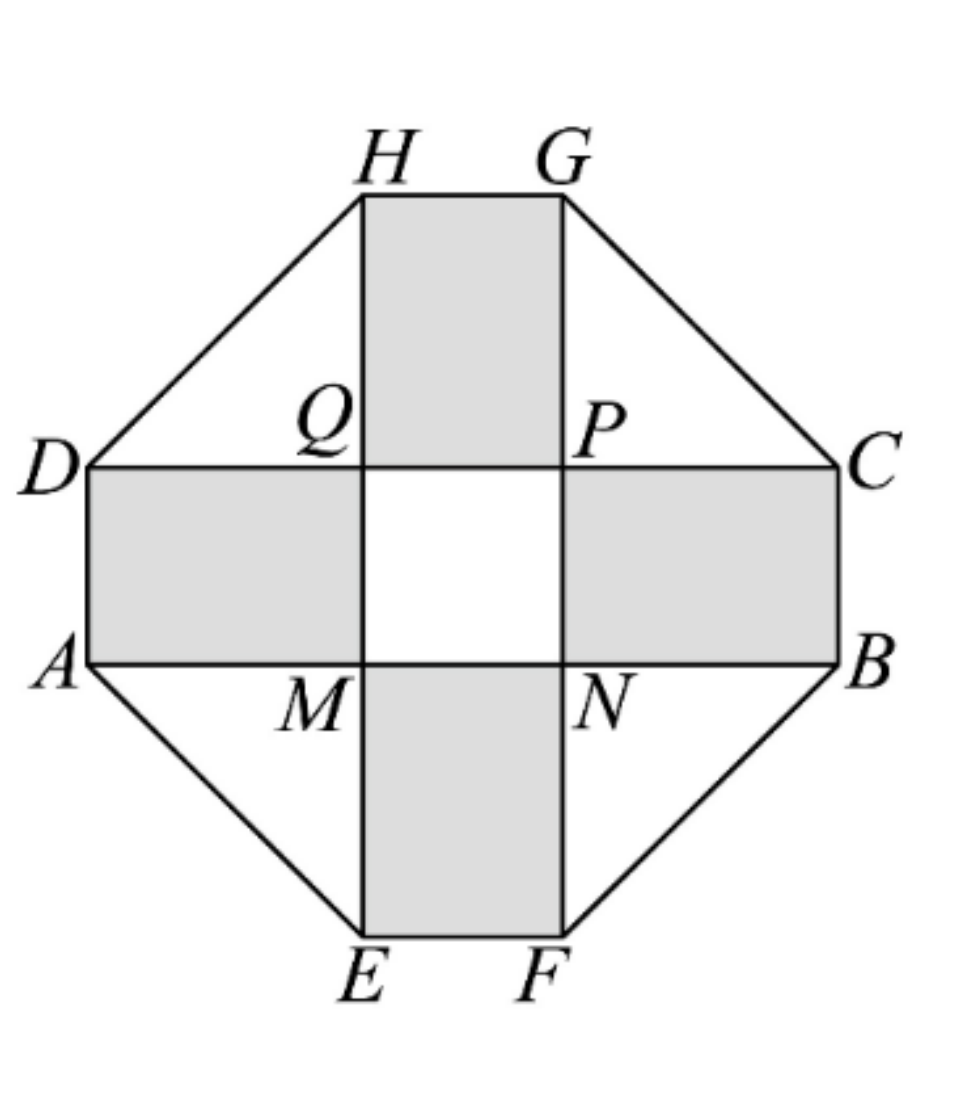
\includegraphics[width=0.34\textwidth]{figures/cross_octagon_h64.png}
\end{center}

\begin{enumerate}[label=(\arabic*)]
\item 设 $DQ$ 长为 $y\mathrm{m}$（$y>0$），用 $x$ 表示 $y$，并求出 $x$ 的取值范围；
\item 如何设计 $AD$ 可使总造价最低，并求出最低造价.
\item 若总造价 $W$ 不超过 69000 元，求 $AD$ 长 $x$ 的取值范围.
\end{enumerate}

\ifanswer
\solbegin
\stepm{(1)}{设 $DQ$ 长为 $y\mathrm{m}$，因为十字形区域面积为 $200\text{m}^2$，}
\step{所以 $4xy+x^2=200$，解得 $y=\dfrac{200-x^2}{4x}=\dfrac{50}{x}-\dfrac x4$；\dots\dots2 分}
\step{因为 $y>0$，所以 $x^2<200$，因为 $x>0$，所以 $0<x<10\sqrt2$.\dots\dots4 分}
\stepm{(2)}{四个矩形地砖面积 $S_{\text{四个矩形}}=4xy=200-x^2$，}
\step{造价 $W_{\text{四个矩形}}=105(200-x^2)$；}
\step{四个三角形草坪面积 $S_{\text{三角形}}=4\times\dfrac12y^2=2\left(\dfrac{50}{x}-\dfrac x4\right)^2=\dfrac{5000}{x^2}+\dfrac{x^2}8-50$，}
\step{造价 $W_{\text{三角形}}=40\left(\dfrac{5000}{x^2}+\dfrac{x^2}8-50\right)$；}
\step{正方形花坛面积 $S_{\text{正方形}}=x^2$，造价 $W_{\text{正方形}}=2100x^2$；}
\step{总造价 $W=W_{\text{四个矩形}}+W_{\text{三角形}}+W_{\text{正方形}}$}
\step{$=105(200-x^2)+40\left(\dfrac{5000}{x^2}+\dfrac{x^2}8-50\right)+2100x^2$，}
\step{化简得 $W=2000x^2+19000+\dfrac{200000}{x^2}$（$0<x<10\sqrt2$）.\dots\dots6 分}
\step{因为 $2000x^2+\dfrac{200000}{x^2}\geqslant40000$，}
\step{当且仅当 $x=\sqrt{10}$（在 $x$ 范围中）时取等号，此时 $W=59000$ 元.}
\step{综上，当 $AD$ 的长为 $\sqrt{10}$ 时，总造价最低，为 59000 元.\dots\dots8 分}
% 原卷 (3) 定义域印作 0<x<2√10，与 (1) 所得 0<x<10√2 不一致，照录（见文件头“原卷笔误”④）
\stepm{(3)}{由（2）得 $W=2000x^2+19000+\dfrac{200000}{x^2}$（$0<x<2\sqrt{10}$）.}
\step{总造价不超过 69000 元，即 $W=2000x^2+19000+\dfrac{200000}{x^2}\leqslant69000$，}
\step{化简得 $x^2+\dfrac{100}{x^2}\leqslant25$，\dots\dots10 分}
\step{即 $(x^2)^2-25x^2+100=(x^2-20)(x^2-5)\leqslant0$，即 $\sqrt5\leqslant x\leqslant2\sqrt5$，}
% 原卷末句“取值范围[√5,2√5]”脱“为”，照录（见文件头“原卷笔误”⑤）
\step{所以 $AD$ 长 $x$ 的取值范围$[\sqrt5,2\sqrt5]$.\dots\dots12 分}
\solend
\fi

\ansspace[10]

\item 设 $a,b,c$ 为实数，集合 $S=\{x\mid(x+a)(x^2+bx+c)=0,x\in\R\}$.

\begin{enumerate}[label=(\arabic*)]
\item 若 $a=1,b=3,c=2$，求集合 $S$；
\item 若 $S=\{-2\}$，求 $a,b,c$ 满足的条件；
\item 设 $T=\{x\mid(ax+1)(cx^2+bx+1)=0,x\in\R\}$，当 $ac\neq0$ 时，如果 $\dfrac12\in S$，$-2\in T$，且
集合 $S,T$ 均恰有两个元素，求三元数对 $(a,b,c)$.
\end{enumerate}

\ifanswer
\solbegin
\stepm{(1)}{若 $a=1,b=3,c=2$，}
\step{则方程 $(x+a)(x^2+bx+c)=0$ 为 $(x+1)(x^2+3x+2)=0$，}
\step{即 $(x+1)^2(x+2)=0$，解得 $x=-1$ 或 $x=-2$，所以 $S=\{-1,-2\}$；}
\stepm{(2)}{由题意得 $-a\in S$，因为 $S=\{-2\}$，所以 $-2$ 是方程 $x+a=0$ 的根，}
\step{即 $-2+a=0$，解得 $a=2$. 由 $S=\{-2\}$，集合 $S$ 有且仅有一个元素，}
\step{即方程 $(x+a)(x^2+bx+c)=0$ 有且仅有一个根，}
\stepm{①}{若 $-2$ 是方程 $x^2+bx+c=0$ 的根，}
\step{则 $\Delta=b^2-4c=0$，且 $-\dfrac b2=-2$，解得 $b=4,c=4$；}
\stepm{②}{若 $-2$ 不是方程 $x^2+bx+c=0$ 的根，则方程 $x^2+bx+c=0$ 无实数根，}
\step{则 $\Delta=b^2-4c<0$，}
\step{综上所述，$\begin{cases}a=2\\ b=4\\ c=4\end{cases}$ 或 $\begin{cases}a=2\\ b^2-4c<0\end{cases}$.}
\stepm{(3)}{$S=\{x\mid(x+a)(x^2+bx+c)=0,x\in\R\}$，}
\step{$T=\{x\mid(ax+1)(cx^2+bx+1)=0,x\in\R\}$，}
\step{由题意得 $a\neq0$ 且 $c\neq0$，则 $-a\in S,-\dfrac1a\in T$，}
\step{且方程 $x^2+bx+c=0$ 与 $cx^2+bx+1=0$ 有相同的判别式 $\Delta=b^2-4c$，}
\step{即两方程根的个数相同. 由集合 $S,T$ 均恰有两个元素，则 $\Delta=b^2-4c\geqslant0$.}
\step{$S=\{x\mid(x+a)(x^2+bx+c)=0,x\in\R\}$，}
\step{因为 $\dfrac12\in S$，所以 $\dfrac12$ 是方程 $x+a=0$ 或 $x^2+bx+c=0$ 的根.}
\step{$T=\{x\mid(ax+1)(cx^2+bx+1)=0,x\in\R\}$，}
\step{由 $-\dfrac1a\in T$，且 $-2\in T$，则 $-2$ 是方程 $ax+1=0$ 或 $cx^2+bx+1=0$ 的根.}
\stepm{①}{当 $a=-\dfrac12$ 时，$\dfrac12$ 是方程 $x+a=0$ 的根，$-a=\dfrac12\in S$，则 $-\dfrac1a=2\in T$，}
\step{又 $-2\in T$，则 $T=\{-2,2\}$，}
\step{由 $T=\left\{x\mid\left(-\dfrac12x+1\right)(cx^2+bx+1)=0,x\in\R\right\}$，}
% 原卷句末为句号，本稿原错作逗号
\step{则 $-2$ 是方程 $cx^2+bx+1=0$ 的根，则 $4c-2b+1=0$.}
\stepm{(i)}{若 $\Delta=b^2-4c=0$，联立 $\begin{cases}4c-2b+1=0\\ b^2-4c=0\end{cases}$ 解得 $b=1,c=\dfrac14$.}
\step{验证：当 $a=-\dfrac12,b=1,c=\dfrac14$ 时，}
\step{$S=\left\{x\mid\left(x-\dfrac12\right)\left(x^2+x+\dfrac14\right)=0,x\in\R\right\}=\left\{-\dfrac12,\dfrac12\right\}$，}
\step{$T=\left\{x\mid\left(-\dfrac12x+1\right)\left(\dfrac14x^2+x+1\right)=0,x\in\R\right\}=\{-2,2\}$，满足题意；}
\stepm{(ii)}{若 $\Delta=b^2-4c>0$，方程 $cx^2+bx+1=0$ 有两个不相等的实数根，}
\step{又 $T=\{-2,2\}$，则方程 $cx^2+bx+1=0$ 的两根必为 $-2$ 和 2.}
\step{由韦达定理得 $\begin{cases}-2+2=-\dfrac bc\\ -2\times2=\dfrac1c\end{cases}$，解得 $b=0,c=-\dfrac14$；}
\step{验证：当 $a=-\dfrac12,b=0,c=-\dfrac14$ 时，}
\step{$S=\left\{x\mid\left(x-\dfrac12\right)\left(x^2-\dfrac14\right)=0,x\in\R\right\}=\left\{-\dfrac12,\dfrac12\right\}$，}
\step{$T=\left\{x\mid\left(-\dfrac12x+1\right)\left(-\dfrac14x^2+1\right)=0,x\in\R\right\}=\{-2,2\}$，满足题意；}
\stepm{②}{当 $a=\dfrac12$ 时，$-\dfrac1a=-2$，即 $-2$ 是方程 $ax+1=0$ 的根，}
\step{则 $-a=-\dfrac12\in S$，又 $\dfrac12\in S$，则 $S=\left\{-\dfrac12,\dfrac12\right\}$，}
\step{$S=\{x\mid(x+a)(x^2+bx+c)=0,x\in\R\}$，}
\step{则 $\dfrac12$ 是方程 $x^2+bx+c=0$ 的根，则 $\dfrac14+\dfrac12b+c=0$，即 $4c+2b+1=0$；}
\stepm{(i)}{若 $\Delta=b^2-4c=0$，联立 $\begin{cases}4c+2b+1=0\\ b^2-4c=0\end{cases}$ 解得 $b=-1,c=\dfrac14$.}
\step{验证：当 $a=\dfrac12,b=-1,c=\dfrac14$ 时，}
\step{$S=\left\{x\mid\left(x+\dfrac12\right)\left(x^2-x+\dfrac14\right)=0,x\in\R\right\}=\left\{-\dfrac12,\dfrac12\right\}$，}
\step{$T=\left\{x\mid\left(\dfrac12x+1\right)\left(\dfrac14x^2-x+1\right)=0,x\in\R\right\}=\{-2,2\}$，满足题意；}
% 原卷作“有两不等的实数根”，本稿原脱“的”
\stepm{(ii)}{若 $\Delta=b^2-4c>0$，方程 $x^2+bx+c=0$ 有两不等的实数根，}
% 原卷句末为句号，本稿原错作逗号
\step{又 $S=\left\{-\dfrac12,\dfrac12\right\}$，则方程 $x^2+bx+c=0$ 的两根必为 $-\dfrac12$ 和 $\dfrac12$.}
\step{由韦达定理得 $\begin{cases}-\dfrac12+\dfrac12=-b\\ -\dfrac12\times\dfrac12=c\end{cases}$，解得 $b=0,c=-\dfrac14$；}
\step{验证：当 $a=\dfrac12,b=0,c=-\dfrac14$ 时，}
\step{$S=\left\{x\mid\left(x+\dfrac12\right)\left(x^2-\dfrac14\right)=0,x\in\R\right\}=\left\{-\dfrac12,\dfrac12\right\}$，}
\step{$T=\left\{x\mid\left(\dfrac12x+1\right)\left(-\dfrac14x^2+1\right)=0,x\in\R\right\}=\{-2,2\}$，满足题意；}
\stepm{③}{当 $a\neq-\dfrac12$ 且 $a\neq\dfrac12$ 时，则 $\dfrac12$ 不是方程 $x+a=0$ 的根，}
\step{$-2$ 也不是方程 $ax+1=0$ 的根.}
% 原卷此句单根而称“两实数根”，语病，照录（见文件头“原卷笔误”⑥）
\step{由 $\dfrac12\in S,-2\in T$，则 $\dfrac12$ 是方程 $x^2+bx+c=0$ 的两实数根，}
\step{且 $-2$ 是方程 $cx^2+bx+1=0$ 的根，则有 $\begin{cases}\dfrac14+\dfrac12b+c=0\\ 4c-2b+1=0\end{cases}$，}
\step{解得 $b=0,c=-\dfrac14$.}
\step{验证：当 $a\neq-\dfrac12$ 且 $a\neq\dfrac12,b=0,c=-\dfrac14$ 时，有 $-a\neq\dfrac12,-a\neq-\dfrac12$.}
\step{$S=\left\{x\mid(x+a)\left(x^2-\dfrac14\right)=0,x\in\R\right\}=\left\{-a,-\dfrac12,\dfrac12\right\}$ 有三个元素，}
\step{故不满足题意；}
\step{综上所述，满足题意的所有三元数对 $(a,b,c)$ 有}
\step{$\left(-\dfrac12,1,\dfrac14\right)$，$\left(-\dfrac12,0,-\dfrac14\right)$，$\left(\dfrac12,-1,\dfrac14\right)$，$\left(\dfrac12,0,-\dfrac14\right)$.}
\solend
\fi

\ansspace*[10]

\end{enumerate}

\end{document}
"
% 紧凑版：xelatex "\def\iscompact{1}% 高一64_格致中学_10月月考.tex
%   —— 高一上数学“2026-2027 年格致中学高一上 10 月月考”（讲评版）
% 试卷版：xelatex 高一64_格致中学_10月月考.tex
% 答案版：xelatex "\def\isanswer{1}\input{高一64_格致中学_10月月考.tex}"
% 紧凑版：xelatex "\def\iscompact{1}\input{高一64_格致中学_10月月考.tex}"
%
% 原始材料：微信公众号“魔都数学加油站”文章，作者破晓，连载“27学年高一64”；
% 原文标题“27学年高一64——2026-2027年上海市格致中学高一上10月月考”；
% 原文链接：https://mp.weixin.qq.com/s/0DfB77nTJf7NdVI_FYXxeA。
% 页面标注发布时间 2026-10-17 21:58（上海）。
% 本次转录只据 `原图/高一64_格致中学_10月月考/` 的 14 张 PNG 逐页读图。
% 正文为 14 张 PNG 页（`01..14.png`）：第 12、13、14 页 2560×3620，
% 第 01—11 页 4762×6735（**同一篇各页分辨率不同**），均按页序读取。
% 14 页全为试卷正文页（卷首标题在第 1 页页顶，卷末解答题第 18 题解析止于第 14 页），
% 无封面页、目录页、二维码或宣传页。粉色斜排“魔都数学加油站”为卷面水印，与公众号页脚一并未录入。
%
% 卷首标题：照卷面印作“2026--2027 年格致中学高一上 10 月月考”，年份区间按全稿惯例排 en dash。
% 原卷只有一行标题、无副标题。
%
% 篇幅与题号：原卷自第 3 题起编号（第 1、2 题不在本卷内）。填空题 3—10（8 题）、
% 选择题 11—14（4 题）、解答题 15—18（4 题），共 16 题。本稿沿用原节与原题号，
% 只改排为全稿统一的大节样式（原卷小节标题为“一、填空题”“二、选择题”“三、解答题”）。
%
% 讲评版：原卷每题下直接印【答案】或【解析】。**只印【答案】的 1 题**（第 5 题），
% 本稿只给 \ans{}；其余 15 题都印【解析】（按全稿口径这类题不另提 \ans{}——第 11、13、14 题
% 的结论写在解析末句（“故选 A”“故选 D”等），亦照录在解析内）。**另有 1 题答案印在题干括号内**——
% 第 12 题（“( B )”，该题无【答案】/【解析】段），本稿按 高一37 第 13 题成例把括号留空、
% 答案另提为 \ans{$B$}。
%
% 副标题：原卷未印副标题。本稿按“知识模块”口径标作“集合与常用逻辑用语、不等式”：
% 16 题中集合与常用逻辑用语 8 题（第 4、9、10、11、12、13、16、18 题），
% 不等式 8 题（含一元二次方程与韦达定理、基本不等式、二次不等式、恒成立、分式不等式：
% 第 3、5、6、7、8、14、15、17 题），两类均达三分之一，故并标。口径同 高一59、高一63。
%
% 与原卷的排版差异：
%   ① 原卷每题下直接印【答案】/【解析】，本稿按全稿惯例将答案与解析置于答案版，试卷版保持干净；
%   ② 原卷未印副标题，本稿按“知识模块”口径补出；
%   ③ 原卷填空横线约三四个字宽，本稿按全稿惯例统一排 \blankline[4.4em]；
%   ④ 原卷实数集排斜体 $R$（第 4、7、8、13、15、18 题）或粗体 $\mathbf{R}$（第 18 题题干与
%      解析共 6 处），整数集排斜体 $Z$（第 9、13 题）或粗体 $\mathbf{Z}$（第 9 题解析末两行），
%      有理数集排粗体 $\mathbf{Q}$（第 13 题选项 A），本稿按全稿惯例统一改用 $\R$、$\Z$、$\Q$
%      （记号归一，粗体／斜体不作区分）；空集记号原卷作 $\varnothing$，照录；
%   ⑤ 第 4 题的补集**原卷用上划线记号 $\bar B$**（题干 1 处、解析 4 处，共 5 处），
%      与全稿惯例的 $\complement_U B$ 不同，本稿照录原卷的 $\bar B$；
%   ⑥ 原卷用描述法时竖线排细竖“$|$”（如 $\{x\mid|x|\geqslant2024\}$ 一类），本稿按全稿惯例排 \mid；
%   ⑦ 第 15—18 题的子问原卷各自另起一行、以“（1）”“（2）”“（3）”标号，本稿按全稿惯例用
%      enumerate 的 (1)(2)(3)；解析中的子问标号一律用 \stepm{(1)}{…}；
%      第 18 题解析中分情形的①②③与分小目的 (i)(ii)，按全稿惯例作 \stepm{①}{…}、\stepm{(i)}{…}；
%   ⑧ 第 13 题解析的“A 选项：”“B 选项：”“C 选项：”“D 选项：”原卷排**加粗**（共 4 处），
%      同 高一63“法一：”成例，本稿排 \stepm{A 选项：}{…} 一类（加粗着色、不改黑色基调），
%      冒号照原卷排全角；
%   ⑨ 第 17 题解析带评分档，原卷在档与档之间排一串点线（“………2 分”），
%      本稿照录为“\dots\dots2 分”一类（同 高一54 成例），共 5 处；
%   ⑩ 选择题的作答括号原卷排半角“(　　)”（第 11、13、14 题括号内空白、第 12 题括号内印 B），
%      本稿按全稿惯例排 \mbox{（\quad）}；选项字母后的句点照原卷排“A.”“B.”；
%   ⑪ 每道解答题原卷未留作答空白，本稿按全稿惯例加 \ansspace（末题用 \ansspace*）；
%   ⑫ 第 17 题题干右侧的十字形八边形示意图，本稿按原卷截图裁出（`figures/cross_octagon_h64.png`，
%      原分辨率裁切，未放大、未用 TikZ 重绘），图内阴影与点名照原卷。
%
% 原卷笔误/存疑（均照录未改，正文对应处另有 % 注）：
%   ① 第 8 题解析末两步自相矛盾：上一步已化为 $\dfrac x{x-1}<0$，下一步却印作
%      “即 $x(x+1)<0$，解得 $-1<x<0$”并给出解集 $(-1,0)$——由 $\dfrac x{x-1}<0$ 应得
%      $x(x-1)<0$、解集 $(0,1)$；已 8 倍放大确认原卷确为 $x+1$ 与 $(-1,0)$，照录未改。
%   ② 第 13 题 D 选项解析“乘法满足结合率”的“率”应为“律”（同段 A、B 选项均作“结合律”）。
%   ③ 第 13 题条件①“任意 $a,b\in G$. 有 $a*b\in G$；”在 $G$ 后印句号（其余三条均以逗号
%      接下文），疑为逗号之误，照录。
%   ④ 第 17 题 (3) 解析把定义域印作 $0<x<2\sqrt{10}$，与 (1) 所得 $0<x<10\sqrt2$ 不一致
%      （疑为 $10\sqrt2$ 之误）；照录未改。
%   ⑤ 第 17 题 (3) 末句“所以 $AD$ 长 $x$ 的取值范围$[\sqrt5,2\sqrt5]$.”脱一个“为”。
%   ⑥ 第 18 题 (3) ③“则 $\dfrac12$ 是方程 $x^2+bx+c=0$ 的**两**实数根”——只有一个数却称
%      “两实数根”，语病；照录。
%
% 插图：第 17 题题干有 1 幅十字形八边形示意图（原卷第 09 页右侧），已按原卷截图排入；
% 其余 13 页无任何图形、无“如图”字样（第 17 题的“图中”均指此图）。
%
\documentclass[a4paper,11pt]{article}
\usepackage{common}

\begin{document}

\examtitlest[3]{2026--2027 年格致中学高一上 10 月月考}{集合与常用逻辑用语、不等式}

\bigsec{一、填空题}

\begin{enumerate}
\setcounter{enumi}{2}

\item 已知一元二次方程 $x^2-nx+5=0$ 的两个实根分别为 $x_1$、$x_2$，且 $\dfrac1{x_1}+\dfrac1{x_2}=1$，则实数 $n$ 的值为\blankline[4.4em].

\ifanswer
\solbegin
\step{$\dfrac1{x_1}+\dfrac1{x_2}=\dfrac{x_1+x_2}{x_1x_2}=\dfrac n5=1$，所以 $n=5$.}
\solend
\fi

\item 全集为 $U=\R$，$A=\{x\mid|x|\geqslant2\}$，$B=\{y\mid y=x^2+1,x\in\R\}$，则 $A\cup\bar B=$\blankline[4.4em].

\ifanswer
\solbegin
\step{由题意得集合 $A=\{x\mid x\geqslant2\text{ 或 }x\leqslant-2\}$，}
\step{因为 $x^2+1\geqslant1$，所以集合 $B=\{x\mid x\geqslant1\}$，所以 $\bar B=\{x\mid x<1\}$，}
\step{则 $A\cup\bar B=\{x\mid x\geqslant2\text{ 或 }x<1\}$.}
\solend
\fi

\item 若 $x>2$，则 $4x+\dfrac1{x-2}$ 的最小值为\blankline[4.4em].

\ifanswer
\ans{$12$}
\fi

\item 已知关于 $x$ 不等式组$\begin{cases}(3x-2)(2x+3)\leqslant0\\ x-a<0\end{cases}$\!没有实数解，则实数 $a$ 的取值范围为\blankline[4.4em].

\ifanswer
\solbegin
\step{由题意得 $\begin{cases}-\dfrac32\leqslant x\leqslant\dfrac23\\ x<a\end{cases}$ 无解，所以 $a\leqslant-\dfrac32$.}
\solend
\fi

\item 若不等式 $\dfrac{x^2-8x+20}{mx^2-mx-1}<0$ 对一切 $x\in\R$ 都成立，则实数 $m$ 的取值范围为\blankline[4.4em].

\ifanswer
\solbegin
\step{因为 $x^2-8x+20=(x-4)^2+4\geqslant4>0$，所以 $mx^2-mx-1<0$，}
\step{当 $m=0$ 时，$mx^2-mx-1=-1<0$，不等式成立；}
\step{设 $y=mx^2-mx-1$，当 $m\neq0$ 时函数 $y$ 为二次函数，$y$ 要恒小于 0，}
\step{抛物线开口向下且与 $x$ 轴没有交点，即 $m<0$ 且 $\Delta<0$，得 $-4<m\leqslant0$，}
\step{故实数 $m$ 的取值范围为 $(-4,0]$.}
\solend
\fi

\item 已知关于 $x$ 的不等式 $\dfrac{ax-1}{x+b}>0$ 的解集为 $\{x\mid-1<x<2\}$，其中 $a$、$b\in\R$，则关于 $x$ 的不等式 $\dfrac{bx+1}{ax+1}<1$ 的解集为\blankline[4.4em].

\ifanswer
\solbegin
\step{不等式 $\dfrac{ax-1}{x+b}>0$ 等价于 $(ax-1)(x+b)>0$，即 $ax^2+(ab-1)x-b>0$，}
\step{所以 $-1$ 和 2 为方程 $ax^2+(ab-1)x-b=0$ 的两根，且 $a<0$，}
\step{由韦达定理得 $\begin{cases}-1+2=-\dfrac{ab-1}a\\ -1\times2=-\dfrac ba\end{cases}$，解得 $\begin{cases}a=-1\\ b=-2\end{cases}$，}
\step{所以原不等式为 $\dfrac{-2x+1}{-x+1}<1\Rightarrow\dfrac{-2x+1}{-x+1}-1<0\Rightarrow\dfrac{-x}{-x+1}<0\Rightarrow\dfrac x{x-1}<0$，}
% 原卷下一步印作“即 x(x+1)<0，解得 -1<x<0”，与上一步 x/(x-1)<0 不等价，
% 照录未改（见文件头“原卷笔误”①）
\step{即 $x(x+1)<0$，解得 $-1<x<0$，即不等式 $\dfrac{bx+1}{ax+1}<1$ 的解集为 $(-1,0)$.}
\solend
\fi

\item 已知集合 $M=\{x\mid|x|\leqslant2024,x\in\Z\}$，集合 $P$ 是 $M$ 的三元子集，即 $P=\{a,b,c\}\subseteq M$，$P$~中元素 $a,b,c$ 满足 $\begin{cases}\dfrac1a+\dfrac1b=\dfrac2c\\ a+c=2b\end{cases}$，则符合要求的集合 $P$ 有\blankline[4.4em]个.

\ifanswer
\solbegin
\step{由 $a+c=2b$，则 $a=2b-c$，代入 $\dfrac1a+\dfrac1b=\dfrac2c$，即 $\dfrac1{2b-c}=\dfrac2c-\dfrac1b=\dfrac{2b-c}{bc}$，}
\step{整理得 $(2b-c)^2=bc$，展开得 $4b^2-5bc+c^2=0$，}
\step{解得 $b=\dfrac c4$ 或 $b=c$（由集合的互异性，舍去），代入 $a+c=2b$ 得 $a=-\dfrac c2$，}
\step{则 $P=\left\{-\dfrac c2,\dfrac c4,c\right\}\subseteq\{x\mid-2024\leqslant x\leqslant2024,x\in\Z\}$，所以 $c$ 为 4 的整数倍，}
\step{且不为 0，则共有 $\dfrac{2024}4\times2=1012$ 个.}
\solend
\fi

\item 已知正整数 $n\geqslant2$，对集合 $\{1,2,3,\cdots,n\}$ 及其每一个非空子集 $X$，记
$X=\{x_1,x_2,\cdots,x_k\}$，其中 $x_1>x_2>\cdots>x_k$，定义一个运算“交替和”
$S_X=x_1-x_2+x_3\cdots+(-1)^{k+1}x_k$. 例如：对于集合 $X=\{9,6,4,2,1\}$，
$S_X=9-6+4-2+1=6$. 则当 $n=7$ 时，集合 $\{1,2,3,\cdots,n\}$ 的所有子集的“交替和”的总
和为\blankline[4.4em].

\ifanswer
\solbegin
\step{由题意得集合 $\{7\}$ 的“交替和”为 7.}
\step{集合 $\{1,2,3,4,5,6,7\}$ 的所有 $2^7$ 个子集中，除去集合 $\{7\}$ 外，}
\step{还有 $2^7-2$ 个非空子集，这 $2^7-2$ 个非空子集中不含元素 7 的集合，}
\step{即 $\{1,2,3,4,5,6\}$ 的非空子集，共有 $2^6-1$ 个，设为 $A_i(i=1,2,\cdots,2^6-1)$；}
\step{则这 $2^7-2$ 个非空子集中含元素 7 的集合，也共有 $2^6-1$ 个，}
\step{这样的集合都可以看成相应地在每个不含 7 的集合中再加上元素 7 得到，}
\step{即 $A_i\cup\{7\}$.}
\step{对 $A_i(i=1,2,\cdots,2^6-1)$ 中的任意集合 $A$，记 $A=\{x_1,x_2,\cdots,x_k\}$，}
\step{则“交替和”$S_A=x_1-x_2+x_3\cdots+(-1)^{k+1}x_k$，其中 $x_1>x_2>\cdots>x_k$，}
\step{由 $7>x_1>x_2>\cdots>x_k$，}
\step{则集合 $A\cup\{7\}$ 的“交替和”为 $7-[x_1-x_2+x_3\cdots+(-1)^{k+1}x_k]$，}
\step{则集合 $A$ 与集合 $A\cup\{7\}$ 的“交替和”之和为 7，下面举例说明：}
\step{如集合 $\{6,5,4,3,2,1\}$ 与集合 $\{7,6,5,4,3,2,1\}$，}
\step{$\{6,5,4,3,2,1\}$ 的“交替和”为 $6-5+4-3+2-1=3$，}
% 原卷此句在页末折为两个印刷行（“……的“交替和”为”／“7-6+5-4+3-2+1=……”），
% 本稿原并作一条，现照原卷拆开（原卷原样两行 / 本稿原错处：并作一行）
\step{$\{7,6,5,4,3,2,1\}$ 的“交替和”为}
\step{$7-6+5-4+3-2+1=7-(6-5+4-3+2-1)=7-3$，}
\step{即集合 $\{6,5,4,3,2,1\}$ 与集合 $\{7,6,5,4,3,2,1\}$ 的“交替和”之和为 7.}
\step{综上，把这 $2^7-2$ 个非空子集两两结组后分别计算每一组中“交替和”之和，}
\step{且每组中“交替和”之和都为 7，共有 $2^6-1$ 组.}
\step{故集合 $\{1,2,3,4,5,6,7\}$ 所有“交替和”之和，}
\step{由各组之和再加集合 $\{7\}$ 的“交替和”7 即可，}
\step{综上所述，当 $n=7$ 时，集合 $\{1,2,3,\cdots,n\}$ 的所有子集的所有“交替和”之和}
\step{为 $7\times(2^6-1)+7=448$.}
\solend
\fi

\end{enumerate}

\bigsec{二、选择题}

\begin{enumerate}
\setcounter{enumi}{10}

\item 若 $a$、$b\in\R$，则“$a<b<0$”是“$a^2>b^2$”的\mbox{（\quad）}条件.

\keepwithprev
A. 充分非必要\qquad B. 必要非充分

C. 充要\qquad D. 既非充分也非必要

\ifanswer
\solbegin
\step{由 $a<b<0\Rightarrow-a>-b>0\Rightarrow(-a)^2>(-b)^2\Rightarrow a^2>b^2$，}
\step{因此由 $a<b<0$ 可以推出 $a^2>b^2$，}
\step{但是当 $a=1$，$b=0$ 时，显然 $a^2>b^2$ 成立，但是 $a<b<0$ 不成立，}
\step{因此由 $a^2>b^2$ 不一定能推出 $a<b<0$，}
\step{因此“$a<b<0$”是“$a^2>b^2$”的充分非必要条件. 故选 $A$.}
\solend
\fi

% 第 12 题答案“B”直接印在题干括号内“(  B  )”，且该题无【答案】/【解析】段；
% 按 高一37 第 13 题的成例括号留空、答案另提为 \ans{}（见文件头）
\item 用反证法证明结论“$a$、$b$、$c$ 至少有一个是正数”时，应假设\mbox{（\quad）}

\keepwithprev
A. $a$、$b$、$c$ 都是正数\qquad B. $a$、$b$、$c$ 都不是正数

C. $a$、$b$、$c$ 至多有一个正数\qquad D. $a$、$b$、$c$ 至多有两个正数

\ifanswer
\ans{$B$}
\fi

\item “群”的概念由数学家伽罗瓦在 19 世纪 30 年代开创，群论虽起源于对代数多项式方程
的研究，但在量子力学、晶体结构学等其他学科中也有十分广泛的应用.“群”的定义是：

设 $G$ 为某种元素组成的一个非空集合，若在 $G$ 内定义一个运算“*”，满足以下条件：

% 原卷条件①在 G 后印句号，疑为逗号之误，照录（见文件头“原卷笔误”③）
①任意 $a,b\in G$. 有 $a*b\in G$；

②如 $a,b,c\in G$，有 $(a*b)*c=a*(b*c)$；

③在 $G$ 中有一个元素 $e$，对任意 $a\in G$，都有 $a*e=e*a=a$，称 $e$ 为 $G$ 的单位元；

④任意 $a\in G$，在 $G$ 中存在唯一确定的 $b$，使 $a*b=b*a=e$，称 $b$ 为 $a$ 的逆元；

此时称 $(G,*)$ 为一个群.

例如实数集 $\R$ 和实数集上的加法运算“+”就构成一个群 $(\R,+)$，其单位元是 0，每一个数
的逆元是其相反数，那么下列说法中，错误的是\mbox{（\quad）}

\keepwithprev
A. $G=\Q$，则 $(G,+)$ 为一个群

B. $G=\{\sqrt2m+\sqrt3n\mid m,n\in\Z\}$，$(G,+)$ 为一个群

C. $G=\{-1,1\}$，则 $(G,\times)$ 为一个群

D. $G=\{x\mid x=2k+1,k\in\Z\}$，则 $(G,\times)$ 为一个群

\ifanswer
\solbegin
\stepm{A 选项：}{有理数的和还是有理数，求和满足结合律，}
\step{设 $a\in\Q$，单位元为 $e$，则 $a+e=a$，故 $e=0$，}
\step{所以每一个数的相反数为其逆元，故 $(G,+)$ 为一个群，选项 A 正确；}
\stepm{B 选项：}{$G=\{\sqrt2m+\sqrt3n\mid m,n\in\Z\}$ 中的任何两个数相加还是属于}
\step{$G=\{\sqrt2m+\sqrt3n\mid m,n\in\Z\}$，求和满足结合律，}
\step{设 $\sqrt2x+\sqrt3y\in G,x,y\in\Z$，单位元为 $e$，}
\step{则 $\sqrt2x+\sqrt3y+e=\sqrt2x+\sqrt3y$，所以 $e=0$，}
\step{每一个数的相反数为其逆元，$(G,+)$ 为一个群，选项 B 正确；}
\stepm{C 选项：}{$G=\{-1,1\}$ 中的两个元素相乘，其积可能为 1 或 $-1$，又 $1\in G,-1\in G$，}
\step{设 $a\in G$，单位元为 $e$，则 $a\times e=a$，故 $e=1,1$ 的逆元为 $1,-1$ 的逆元为 $-1$，}
\step{所以 $(G,\times)$ 为一个群，选项 C 正确；}
% 原卷“乘法满足结合率”的“率”应为“律”（同段 A、B 选项均作“结合律”），照录（见文件头“原卷笔误”②）
\stepm{D 选项：}{两个奇数相乘还是奇数，乘法满足结合率，}
\step{设 $a\in G$，单位元为 $e$，则 $a\times e=a$，故 $e=1$，}
\step{又 $3\in G$，故存在 $b\in G$，使得 $3b=1$，则 $b=\dfrac13$，矛盾，}
\step{故 $(G,\times)$ 不为一个群，选项 D 错误.}
\step{故选 $D$.}
\solend
\fi

\item 已知 $a$、$b$、$c\in\R$，若关于 $x$ 的不等式 $0\leqslant x+\dfrac ax+b\leqslant\dfrac cx-1$ 的解集为 $[x_1,x_2]\cup\{x_3\}$
（$x_3>x_2>x_1>0$），则\mbox{（\quad）}

\keepwithprev
A. 不存在有序数组 $(a,b,c)$，使得 $x_2-x_1=1$

B. 存在唯一有序数组 $(a,b,c)$，使得 $x_2-x_1=1$

C. 有且只有两组有序数组 $(a,b,c)$，使得 $x_2-x_1=1$

D. 存在无穷多组有序数组 $(a,b,c)$，使得 $x_2-x_1=1$

\ifanswer
\solbegin
\step{因为不等式 $0\leqslant x+\dfrac ax+b\leqslant\dfrac cx-1$ 的解集为 $[x_1,x_2]\cup\{x_3\}$（$x_3>x_2>x_1>0$），}
\step{所以 $0\leqslant x^2+bx+a\leqslant c-x$ 在 $[x_1,x_2]\cup\{x_3\}$ 上成立，}
\step{假设 $x_1=m$，$x_2=m+1$，$x_3=n$，}
\step{则 $c-n=0=n^2+bn+a$，由 $x_3$ 为一个独立的数得出，}
\step{所以 $n=c$，且 $m+1$ 与 $n$ 为方程 $x^2+bx+a=0$ 的两个根，}
\step{因为 $x_3>x_2>x_1>0$，所以 $-b=m+n+1=m+c+1$，$a=mn+n=mc+c$，}
\step{所以 $b=-m-c-1$，}
\step{且点 $(x_1,x_1^2+bx_1+a)$ 为 $y=x^2+bx+a$ 与 $y=c-x$ 的左交点，}
\step{所以 $m^2+bm+a=c-m$ 且 $b=-m-c-1$，$a=mc+c$，}
\step{故 $m^2+bm+a=m^2-m^2-mc-m+mc+c=c-m$，所以 $c-m=c-m$ 恒成立，}
\step{所以不论 $a$、$b$、$c$ 取何值，$x_2-x_1=1$ 恒成立，}
\step{即存在无穷多组有序数组 $(a,b,c)$，使得 $x_2-x_1=1$，}
\step{故选项 $A$、$B$、$C$ 错误，选项 $D$ 正确. 故选 $D$.}
\solend
\fi

\end{enumerate}

\bigsec{三、解答题}

\begin{enumerate}
\setcounter{enumi}{14}

\item 已知函数 $f(x)=(a-1)x^2-ax+1$，$a\in\R$.

\begin{enumerate}[label=(\arabic*)]
\item 若不等式 $f(x)<0$ 的解集为 $\left(\dfrac13,1\right)$，求实数 $a$ 的值；
\item 当 $a>1$ 时，解关于 $x$ 的不等式 $f(x)\geqslant0$.
\end{enumerate}

\ifanswer
\solbegin
\stepm{(1)}{因为不等式 $f(x)<0$ 的解集为 $\left(\dfrac13,1\right)$，}
\step{所以不等式对应的方程 $(a-1)x^2-ax+1=0$ 的两根分别为 $\dfrac13$、1，}
\step{由根与系数的关系得 $\begin{cases}1+\dfrac13=\dfrac a{a-1}\\ 1\times\dfrac13=\dfrac1{a-1}\end{cases}$，解得 $a=4$；}
\stepm{(2)}{不等式 $(a-1)x^2-ax+1\geqslant0$（$a>1$）可化为 $(x-1)[(a-1)x-1]\geqslant0$，}
\step{不等式对应方程的两根为 $x_1=1$，$x_2=\dfrac1{a-1}$，}
\step{①当 $\dfrac1{a-1}=1$，即 $a=2$ 时，不等式为 $(x-1)^2\geqslant0$，解集为 $\R$；}
\step{②当 $\dfrac1{a-1}>1$，即 $1<a<2$ 时，解不等式得 $x\leqslant1$ 或 $x\geqslant\dfrac1{a-1}$；}
\step{③当 $\dfrac1{a-1}<1$，即 $a>2$ 时，解不等式得 $x\leqslant\dfrac1{a-1}$ 或 $x\geqslant1$；}
\step{综上，$a=2$ 时，不等式的解集为 $\R$，}
\step{$1<a<2$ 时，不等式的解集为 $(-\infty,1]\cup\left[\dfrac1{a-1},+\infty\right)$，}
\step{$a>2$ 时，不等式的解集为 $\left(-\infty,\dfrac1{a-1}\right]\cup[1,+\infty)$.}
\solend
\fi

\ansspace[6]

\item 若集合 $A=\{x\mid x^2+5x-6=0\}$，$B=\{x\mid x^2+2(m+1)x+m^2-3=0\}$.

\begin{enumerate}[label=(\arabic*)]
\item 若 $m=0$，写出 $A\cup B$ 的子集个数；
\item 若 $A\cap B=B$，求实数 $m$ 的取值范围.
\end{enumerate}

\ifanswer
\solbegin
\stepm{(1)}{当 $m=0$ 时，$B=\{1,-3\}$，}
\step{因为 $A=\{x\mid x^2+5x-6=0\}=\{-6,1\}$，}
\step{所以 $A\cup B=\{-6,-3,1\}$，集合元素个数为 3 个，}
\step{故 $A\cup B$ 的子集个数为 $2^3=8$.}
\stepm{(2)}{因为 $A\cap B=B$，所以 $B\subseteq A$，}
\step{$\Delta=4(m+1)^2-4(m^2-3)=8m+16$，}
\step{当 $\Delta<0$，即 $m<-2$ 时，$B=\varnothing$，符合题意，}
\step{当 $\Delta=0$，即 $m=-2$ 时，$B=\{1\}$，符合题意，}
\step{当 $\Delta>0$，即 $m>-2$ 时，若 $B\subseteq A$，则 $B=\{-6,1\}$，}
\step{即 $\begin{cases}-2(m+1)=-5\\ m^2-3=-6\end{cases}$，方程组无解，}
\step{综上所述，$m$ 的取值范围为 $(-\infty,-2]$.}
\solend
\fi

\ansspace[6]

\item 2025 年上海奇迹花园国际艺术花展于 9 月 20 日正式启幕，本次花展首次实现沉浸 IP
展、花卉景观、跨界艺术、光影夜花园四展合一，为市民游客打造一个可游、可赏、可感
的秋季治愈系童话世界. 某公园受此启发打算设计一个八边形活动区域，该区域的主体造
型平面图是由两个相同的矩形 $ABCD$ 和 $EFGH$ 构成的十字形地域，十字形的面积为
$200\text{m}^2$. 计划在正方形 $MNPQ$ 上建一座花坛，造价为 2100 元$/\text{m}^2$；在四个相同的矩形
（图中阴影部分）上铺地砖，造价为 105 元$/\text{m}^2$；再在四个空角（图中四个三角
形）上铺草坪，造价为 40 元$/\text{m}^2$. 设 $AD$ 长为 $x\mathrm{m}$（$x>0$），总造价为 $W$ 元，求：

\begin{center}
% 插图取自原卷第 09 页右侧截图（原分辨率裁切，未用 TikZ 重绘），阴影与点名照原卷
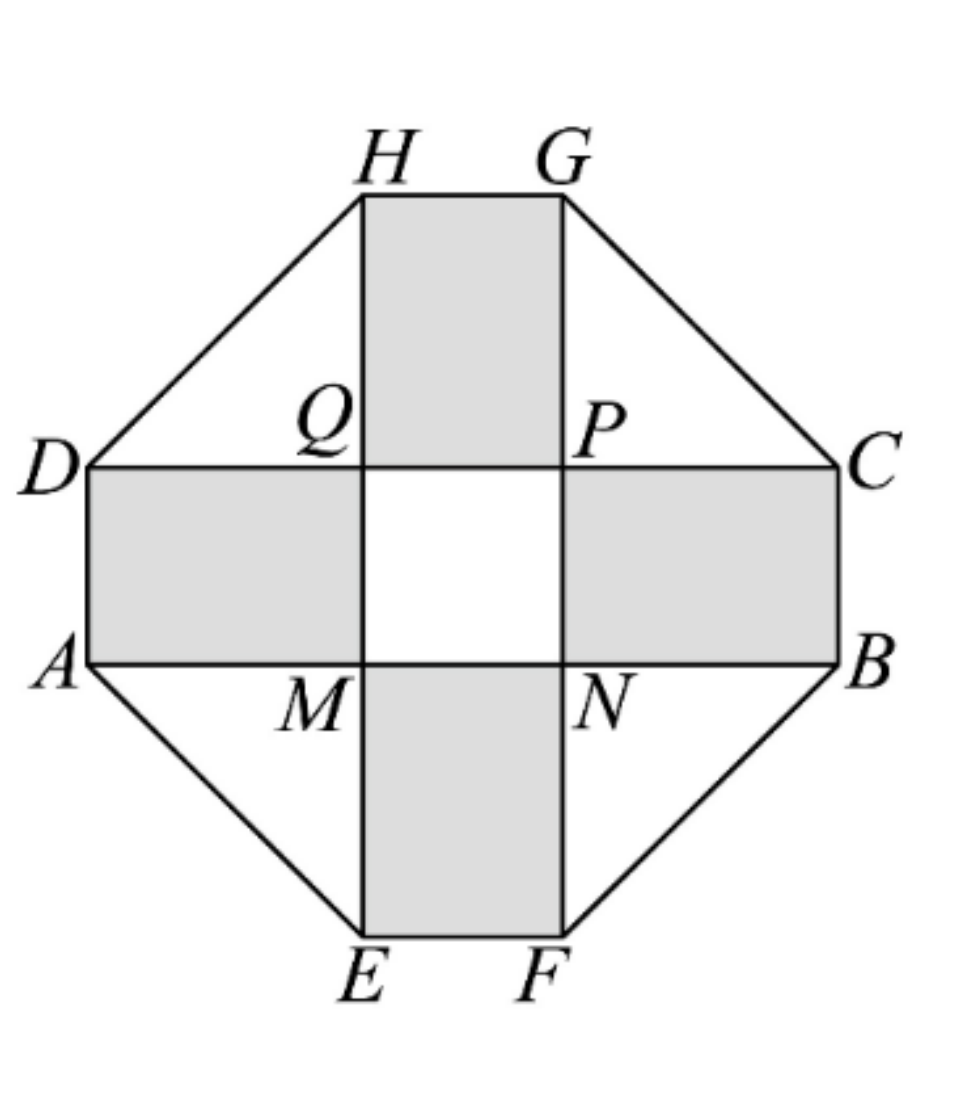
\includegraphics[width=0.34\textwidth]{figures/cross_octagon_h64.png}
\end{center}

\begin{enumerate}[label=(\arabic*)]
\item 设 $DQ$ 长为 $y\mathrm{m}$（$y>0$），用 $x$ 表示 $y$，并求出 $x$ 的取值范围；
\item 如何设计 $AD$ 可使总造价最低，并求出最低造价.
\item 若总造价 $W$ 不超过 69000 元，求 $AD$ 长 $x$ 的取值范围.
\end{enumerate}

\ifanswer
\solbegin
\stepm{(1)}{设 $DQ$ 长为 $y\mathrm{m}$，因为十字形区域面积为 $200\text{m}^2$，}
\step{所以 $4xy+x^2=200$，解得 $y=\dfrac{200-x^2}{4x}=\dfrac{50}{x}-\dfrac x4$；\dots\dots2 分}
\step{因为 $y>0$，所以 $x^2<200$，因为 $x>0$，所以 $0<x<10\sqrt2$.\dots\dots4 分}
\stepm{(2)}{四个矩形地砖面积 $S_{\text{四个矩形}}=4xy=200-x^2$，}
\step{造价 $W_{\text{四个矩形}}=105(200-x^2)$；}
\step{四个三角形草坪面积 $S_{\text{三角形}}=4\times\dfrac12y^2=2\left(\dfrac{50}{x}-\dfrac x4\right)^2=\dfrac{5000}{x^2}+\dfrac{x^2}8-50$，}
\step{造价 $W_{\text{三角形}}=40\left(\dfrac{5000}{x^2}+\dfrac{x^2}8-50\right)$；}
\step{正方形花坛面积 $S_{\text{正方形}}=x^2$，造价 $W_{\text{正方形}}=2100x^2$；}
\step{总造价 $W=W_{\text{四个矩形}}+W_{\text{三角形}}+W_{\text{正方形}}$}
\step{$=105(200-x^2)+40\left(\dfrac{5000}{x^2}+\dfrac{x^2}8-50\right)+2100x^2$，}
\step{化简得 $W=2000x^2+19000+\dfrac{200000}{x^2}$（$0<x<10\sqrt2$）.\dots\dots6 分}
\step{因为 $2000x^2+\dfrac{200000}{x^2}\geqslant40000$，}
\step{当且仅当 $x=\sqrt{10}$（在 $x$ 范围中）时取等号，此时 $W=59000$ 元.}
\step{综上，当 $AD$ 的长为 $\sqrt{10}$ 时，总造价最低，为 59000 元.\dots\dots8 分}
% 原卷 (3) 定义域印作 0<x<2√10，与 (1) 所得 0<x<10√2 不一致，照录（见文件头“原卷笔误”④）
\stepm{(3)}{由（2）得 $W=2000x^2+19000+\dfrac{200000}{x^2}$（$0<x<2\sqrt{10}$）.}
\step{总造价不超过 69000 元，即 $W=2000x^2+19000+\dfrac{200000}{x^2}\leqslant69000$，}
\step{化简得 $x^2+\dfrac{100}{x^2}\leqslant25$，\dots\dots10 分}
\step{即 $(x^2)^2-25x^2+100=(x^2-20)(x^2-5)\leqslant0$，即 $\sqrt5\leqslant x\leqslant2\sqrt5$，}
% 原卷末句“取值范围[√5,2√5]”脱“为”，照录（见文件头“原卷笔误”⑤）
\step{所以 $AD$ 长 $x$ 的取值范围$[\sqrt5,2\sqrt5]$.\dots\dots12 分}
\solend
\fi

\ansspace[10]

\item 设 $a,b,c$ 为实数，集合 $S=\{x\mid(x+a)(x^2+bx+c)=0,x\in\R\}$.

\begin{enumerate}[label=(\arabic*)]
\item 若 $a=1,b=3,c=2$，求集合 $S$；
\item 若 $S=\{-2\}$，求 $a,b,c$ 满足的条件；
\item 设 $T=\{x\mid(ax+1)(cx^2+bx+1)=0,x\in\R\}$，当 $ac\neq0$ 时，如果 $\dfrac12\in S$，$-2\in T$，且
集合 $S,T$ 均恰有两个元素，求三元数对 $(a,b,c)$.
\end{enumerate}

\ifanswer
\solbegin
\stepm{(1)}{若 $a=1,b=3,c=2$，}
\step{则方程 $(x+a)(x^2+bx+c)=0$ 为 $(x+1)(x^2+3x+2)=0$，}
\step{即 $(x+1)^2(x+2)=0$，解得 $x=-1$ 或 $x=-2$，所以 $S=\{-1,-2\}$；}
\stepm{(2)}{由题意得 $-a\in S$，因为 $S=\{-2\}$，所以 $-2$ 是方程 $x+a=0$ 的根，}
\step{即 $-2+a=0$，解得 $a=2$. 由 $S=\{-2\}$，集合 $S$ 有且仅有一个元素，}
\step{即方程 $(x+a)(x^2+bx+c)=0$ 有且仅有一个根，}
\stepm{①}{若 $-2$ 是方程 $x^2+bx+c=0$ 的根，}
\step{则 $\Delta=b^2-4c=0$，且 $-\dfrac b2=-2$，解得 $b=4,c=4$；}
\stepm{②}{若 $-2$ 不是方程 $x^2+bx+c=0$ 的根，则方程 $x^2+bx+c=0$ 无实数根，}
\step{则 $\Delta=b^2-4c<0$，}
\step{综上所述，$\begin{cases}a=2\\ b=4\\ c=4\end{cases}$ 或 $\begin{cases}a=2\\ b^2-4c<0\end{cases}$.}
\stepm{(3)}{$S=\{x\mid(x+a)(x^2+bx+c)=0,x\in\R\}$，}
\step{$T=\{x\mid(ax+1)(cx^2+bx+1)=0,x\in\R\}$，}
\step{由题意得 $a\neq0$ 且 $c\neq0$，则 $-a\in S,-\dfrac1a\in T$，}
\step{且方程 $x^2+bx+c=0$ 与 $cx^2+bx+1=0$ 有相同的判别式 $\Delta=b^2-4c$，}
\step{即两方程根的个数相同. 由集合 $S,T$ 均恰有两个元素，则 $\Delta=b^2-4c\geqslant0$.}
\step{$S=\{x\mid(x+a)(x^2+bx+c)=0,x\in\R\}$，}
\step{因为 $\dfrac12\in S$，所以 $\dfrac12$ 是方程 $x+a=0$ 或 $x^2+bx+c=0$ 的根.}
\step{$T=\{x\mid(ax+1)(cx^2+bx+1)=0,x\in\R\}$，}
\step{由 $-\dfrac1a\in T$，且 $-2\in T$，则 $-2$ 是方程 $ax+1=0$ 或 $cx^2+bx+1=0$ 的根.}
\stepm{①}{当 $a=-\dfrac12$ 时，$\dfrac12$ 是方程 $x+a=0$ 的根，$-a=\dfrac12\in S$，则 $-\dfrac1a=2\in T$，}
\step{又 $-2\in T$，则 $T=\{-2,2\}$，}
\step{由 $T=\left\{x\mid\left(-\dfrac12x+1\right)(cx^2+bx+1)=0,x\in\R\right\}$，}
% 原卷句末为句号，本稿原错作逗号
\step{则 $-2$ 是方程 $cx^2+bx+1=0$ 的根，则 $4c-2b+1=0$.}
\stepm{(i)}{若 $\Delta=b^2-4c=0$，联立 $\begin{cases}4c-2b+1=0\\ b^2-4c=0\end{cases}$ 解得 $b=1,c=\dfrac14$.}
\step{验证：当 $a=-\dfrac12,b=1,c=\dfrac14$ 时，}
\step{$S=\left\{x\mid\left(x-\dfrac12\right)\left(x^2+x+\dfrac14\right)=0,x\in\R\right\}=\left\{-\dfrac12,\dfrac12\right\}$，}
\step{$T=\left\{x\mid\left(-\dfrac12x+1\right)\left(\dfrac14x^2+x+1\right)=0,x\in\R\right\}=\{-2,2\}$，满足题意；}
\stepm{(ii)}{若 $\Delta=b^2-4c>0$，方程 $cx^2+bx+1=0$ 有两个不相等的实数根，}
\step{又 $T=\{-2,2\}$，则方程 $cx^2+bx+1=0$ 的两根必为 $-2$ 和 2.}
\step{由韦达定理得 $\begin{cases}-2+2=-\dfrac bc\\ -2\times2=\dfrac1c\end{cases}$，解得 $b=0,c=-\dfrac14$；}
\step{验证：当 $a=-\dfrac12,b=0,c=-\dfrac14$ 时，}
\step{$S=\left\{x\mid\left(x-\dfrac12\right)\left(x^2-\dfrac14\right)=0,x\in\R\right\}=\left\{-\dfrac12,\dfrac12\right\}$，}
\step{$T=\left\{x\mid\left(-\dfrac12x+1\right)\left(-\dfrac14x^2+1\right)=0,x\in\R\right\}=\{-2,2\}$，满足题意；}
\stepm{②}{当 $a=\dfrac12$ 时，$-\dfrac1a=-2$，即 $-2$ 是方程 $ax+1=0$ 的根，}
\step{则 $-a=-\dfrac12\in S$，又 $\dfrac12\in S$，则 $S=\left\{-\dfrac12,\dfrac12\right\}$，}
\step{$S=\{x\mid(x+a)(x^2+bx+c)=0,x\in\R\}$，}
\step{则 $\dfrac12$ 是方程 $x^2+bx+c=0$ 的根，则 $\dfrac14+\dfrac12b+c=0$，即 $4c+2b+1=0$；}
\stepm{(i)}{若 $\Delta=b^2-4c=0$，联立 $\begin{cases}4c+2b+1=0\\ b^2-4c=0\end{cases}$ 解得 $b=-1,c=\dfrac14$.}
\step{验证：当 $a=\dfrac12,b=-1,c=\dfrac14$ 时，}
\step{$S=\left\{x\mid\left(x+\dfrac12\right)\left(x^2-x+\dfrac14\right)=0,x\in\R\right\}=\left\{-\dfrac12,\dfrac12\right\}$，}
\step{$T=\left\{x\mid\left(\dfrac12x+1\right)\left(\dfrac14x^2-x+1\right)=0,x\in\R\right\}=\{-2,2\}$，满足题意；}
% 原卷作“有两不等的实数根”，本稿原脱“的”
\stepm{(ii)}{若 $\Delta=b^2-4c>0$，方程 $x^2+bx+c=0$ 有两不等的实数根，}
% 原卷句末为句号，本稿原错作逗号
\step{又 $S=\left\{-\dfrac12,\dfrac12\right\}$，则方程 $x^2+bx+c=0$ 的两根必为 $-\dfrac12$ 和 $\dfrac12$.}
\step{由韦达定理得 $\begin{cases}-\dfrac12+\dfrac12=-b\\ -\dfrac12\times\dfrac12=c\end{cases}$，解得 $b=0,c=-\dfrac14$；}
\step{验证：当 $a=\dfrac12,b=0,c=-\dfrac14$ 时，}
\step{$S=\left\{x\mid\left(x+\dfrac12\right)\left(x^2-\dfrac14\right)=0,x\in\R\right\}=\left\{-\dfrac12,\dfrac12\right\}$，}
\step{$T=\left\{x\mid\left(\dfrac12x+1\right)\left(-\dfrac14x^2+1\right)=0,x\in\R\right\}=\{-2,2\}$，满足题意；}
\stepm{③}{当 $a\neq-\dfrac12$ 且 $a\neq\dfrac12$ 时，则 $\dfrac12$ 不是方程 $x+a=0$ 的根，}
\step{$-2$ 也不是方程 $ax+1=0$ 的根.}
% 原卷此句单根而称“两实数根”，语病，照录（见文件头“原卷笔误”⑥）
\step{由 $\dfrac12\in S,-2\in T$，则 $\dfrac12$ 是方程 $x^2+bx+c=0$ 的两实数根，}
\step{且 $-2$ 是方程 $cx^2+bx+1=0$ 的根，则有 $\begin{cases}\dfrac14+\dfrac12b+c=0\\ 4c-2b+1=0\end{cases}$，}
\step{解得 $b=0,c=-\dfrac14$.}
\step{验证：当 $a\neq-\dfrac12$ 且 $a\neq\dfrac12,b=0,c=-\dfrac14$ 时，有 $-a\neq\dfrac12,-a\neq-\dfrac12$.}
\step{$S=\left\{x\mid(x+a)\left(x^2-\dfrac14\right)=0,x\in\R\right\}=\left\{-a,-\dfrac12,\dfrac12\right\}$ 有三个元素，}
\step{故不满足题意；}
\step{综上所述，满足题意的所有三元数对 $(a,b,c)$ 有}
\step{$\left(-\dfrac12,1,\dfrac14\right)$，$\left(-\dfrac12,0,-\dfrac14\right)$，$\left(\dfrac12,-1,\dfrac14\right)$，$\left(\dfrac12,0,-\dfrac14\right)$.}
\solend
\fi

\ansspace*[10]

\end{enumerate}

\end{document}
"
%
% 原始材料：微信公众号“魔都数学加油站”文章，作者破晓，连载“27学年高一64”；
% 原文标题“27学年高一64——2026-2027年上海市格致中学高一上10月月考”；
% 原文链接：https://mp.weixin.qq.com/s/0DfB77nTJf7NdVI_FYXxeA。
% 页面标注发布时间 2026-10-17 21:58（上海）。
% 本次转录只据 `原图/高一64_格致中学_10月月考/` 的 14 张 PNG 逐页读图。
% 正文为 14 张 PNG 页（`01..14.png`）：第 12、13、14 页 2560×3620，
% 第 01—11 页 4762×6735（**同一篇各页分辨率不同**），均按页序读取。
% 14 页全为试卷正文页（卷首标题在第 1 页页顶，卷末解答题第 18 题解析止于第 14 页），
% 无封面页、目录页、二维码或宣传页。粉色斜排“魔都数学加油站”为卷面水印，与公众号页脚一并未录入。
%
% 卷首标题：照卷面印作“2026--2027 年格致中学高一上 10 月月考”，年份区间按全稿惯例排 en dash。
% 原卷只有一行标题、无副标题。
%
% 篇幅与题号：原卷自第 3 题起编号（第 1、2 题不在本卷内）。填空题 3—10（8 题）、
% 选择题 11—14（4 题）、解答题 15—18（4 题），共 16 题。本稿沿用原节与原题号，
% 只改排为全稿统一的大节样式（原卷小节标题为“一、填空题”“二、选择题”“三、解答题”）。
%
% 讲评版：原卷每题下直接印【答案】或【解析】。**只印【答案】的 1 题**（第 5 题），
% 本稿只给 \ans{}；其余 15 题都印【解析】（按全稿口径这类题不另提 \ans{}——第 11、13、14 题
% 的结论写在解析末句（“故选 A”“故选 D”等），亦照录在解析内）。**另有 1 题答案印在题干括号内**——
% 第 12 题（“( B )”，该题无【答案】/【解析】段），本稿按 高一37 第 13 题成例把括号留空、
% 答案另提为 \ans{$B$}。
%
% 副标题：原卷未印副标题。本稿按“知识模块”口径标作“集合与常用逻辑用语、不等式”：
% 16 题中集合与常用逻辑用语 8 题（第 4、9、10、11、12、13、16、18 题），
% 不等式 8 题（含一元二次方程与韦达定理、基本不等式、二次不等式、恒成立、分式不等式：
% 第 3、5、6、7、8、14、15、17 题），两类均达三分之一，故并标。口径同 高一59、高一63。
%
% 与原卷的排版差异：
%   ① 原卷每题下直接印【答案】/【解析】，本稿按全稿惯例将答案与解析置于答案版，试卷版保持干净；
%   ② 原卷未印副标题，本稿按“知识模块”口径补出；
%   ③ 原卷填空横线约三四个字宽，本稿按全稿惯例统一排 \blankline[4.4em]；
%   ④ 原卷实数集排斜体 $R$（第 4、7、8、13、15、18 题）或粗体 $\mathbf{R}$（第 18 题题干与
%      解析共 6 处），整数集排斜体 $Z$（第 9、13 题）或粗体 $\mathbf{Z}$（第 9 题解析末两行），
%      有理数集排粗体 $\mathbf{Q}$（第 13 题选项 A），本稿按全稿惯例统一改用 $\R$、$\Z$、$\Q$
%      （记号归一，粗体／斜体不作区分）；空集记号原卷作 $\varnothing$，照录；
%   ⑤ 第 4 题的补集**原卷用上划线记号 $\bar B$**（题干 1 处、解析 4 处，共 5 处），
%      与全稿惯例的 $\complement_U B$ 不同，本稿照录原卷的 $\bar B$；
%   ⑥ 原卷用描述法时竖线排细竖“$|$”（如 $\{x\mid|x|\geqslant2024\}$ 一类），本稿按全稿惯例排 \mid；
%   ⑦ 第 15—18 题的子问原卷各自另起一行、以“（1）”“（2）”“（3）”标号，本稿按全稿惯例用
%      enumerate 的 (1)(2)(3)；解析中的子问标号一律用 \stepm{(1)}{…}；
%      第 18 题解析中分情形的①②③与分小目的 (i)(ii)，按全稿惯例作 \stepm{①}{…}、\stepm{(i)}{…}；
%   ⑧ 第 13 题解析的“A 选项：”“B 选项：”“C 选项：”“D 选项：”原卷排**加粗**（共 4 处），
%      同 高一63“法一：”成例，本稿排 \stepm{A 选项：}{…} 一类（加粗着色、不改黑色基调），
%      冒号照原卷排全角；
%   ⑨ 第 17 题解析带评分档，原卷在档与档之间排一串点线（“………2 分”），
%      本稿照录为“\dots\dots2 分”一类（同 高一54 成例），共 5 处；
%   ⑩ 选择题的作答括号原卷排半角“(　　)”（第 11、13、14 题括号内空白、第 12 题括号内印 B），
%      本稿按全稿惯例排 \mbox{（\quad）}；选项字母后的句点照原卷排“A.”“B.”；
%   ⑪ 每道解答题原卷未留作答空白，本稿按全稿惯例加 \ansspace（末题用 \ansspace*）；
%   ⑫ 第 17 题题干右侧的十字形八边形示意图，本稿按原卷截图裁出（`figures/cross_octagon_h64.png`，
%      原分辨率裁切，未放大、未用 TikZ 重绘），图内阴影与点名照原卷。
%
% 原卷笔误/存疑（均照录未改，正文对应处另有 % 注）：
%   ① 第 8 题解析末两步自相矛盾：上一步已化为 $\dfrac x{x-1}<0$，下一步却印作
%      “即 $x(x+1)<0$，解得 $-1<x<0$”并给出解集 $(-1,0)$——由 $\dfrac x{x-1}<0$ 应得
%      $x(x-1)<0$、解集 $(0,1)$；已 8 倍放大确认原卷确为 $x+1$ 与 $(-1,0)$，照录未改。
%   ② 第 13 题 D 选项解析“乘法满足结合率”的“率”应为“律”（同段 A、B 选项均作“结合律”）。
%   ③ 第 13 题条件①“任意 $a,b\in G$. 有 $a*b\in G$；”在 $G$ 后印句号（其余三条均以逗号
%      接下文），疑为逗号之误，照录。
%   ④ 第 17 题 (3) 解析把定义域印作 $0<x<2\sqrt{10}$，与 (1) 所得 $0<x<10\sqrt2$ 不一致
%      （疑为 $10\sqrt2$ 之误）；照录未改。
%   ⑤ 第 17 题 (3) 末句“所以 $AD$ 长 $x$ 的取值范围$[\sqrt5,2\sqrt5]$.”脱一个“为”。
%   ⑥ 第 18 题 (3) ③“则 $\dfrac12$ 是方程 $x^2+bx+c=0$ 的**两**实数根”——只有一个数却称
%      “两实数根”，语病；照录。
%
% 插图：第 17 题题干有 1 幅十字形八边形示意图（原卷第 09 页右侧），已按原卷截图排入；
% 其余 13 页无任何图形、无“如图”字样（第 17 题的“图中”均指此图）。
%
\documentclass[a4paper,11pt]{article}
\usepackage{common}

\begin{document}

\examtitlest[3]{2026--2027 年格致中学高一上 10 月月考}{集合与常用逻辑用语、不等式}

\bigsec{一、填空题}

\begin{enumerate}
\setcounter{enumi}{2}

\item 已知一元二次方程 $x^2-nx+5=0$ 的两个实根分别为 $x_1$、$x_2$，且 $\dfrac1{x_1}+\dfrac1{x_2}=1$，则实数 $n$ 的值为\blankline[4.4em].

\ifanswer
\solbegin
\step{$\dfrac1{x_1}+\dfrac1{x_2}=\dfrac{x_1+x_2}{x_1x_2}=\dfrac n5=1$，所以 $n=5$.}
\solend
\fi

\item 全集为 $U=\R$，$A=\{x\mid|x|\geqslant2\}$，$B=\{y\mid y=x^2+1,x\in\R\}$，则 $A\cup\bar B=$\blankline[4.4em].

\ifanswer
\solbegin
\step{由题意得集合 $A=\{x\mid x\geqslant2\text{ 或 }x\leqslant-2\}$，}
\step{因为 $x^2+1\geqslant1$，所以集合 $B=\{x\mid x\geqslant1\}$，所以 $\bar B=\{x\mid x<1\}$，}
\step{则 $A\cup\bar B=\{x\mid x\geqslant2\text{ 或 }x<1\}$.}
\solend
\fi

\item 若 $x>2$，则 $4x+\dfrac1{x-2}$ 的最小值为\blankline[4.4em].

\ifanswer
\ans{$12$}
\fi

\item 已知关于 $x$ 不等式组$\begin{cases}(3x-2)(2x+3)\leqslant0\\ x-a<0\end{cases}$\!没有实数解，则实数 $a$ 的取值范围为\blankline[4.4em].

\ifanswer
\solbegin
\step{由题意得 $\begin{cases}-\dfrac32\leqslant x\leqslant\dfrac23\\ x<a\end{cases}$ 无解，所以 $a\leqslant-\dfrac32$.}
\solend
\fi

\item 若不等式 $\dfrac{x^2-8x+20}{mx^2-mx-1}<0$ 对一切 $x\in\R$ 都成立，则实数 $m$ 的取值范围为\blankline[4.4em].

\ifanswer
\solbegin
\step{因为 $x^2-8x+20=(x-4)^2+4\geqslant4>0$，所以 $mx^2-mx-1<0$，}
\step{当 $m=0$ 时，$mx^2-mx-1=-1<0$，不等式成立；}
\step{设 $y=mx^2-mx-1$，当 $m\neq0$ 时函数 $y$ 为二次函数，$y$ 要恒小于 0，}
\step{抛物线开口向下且与 $x$ 轴没有交点，即 $m<0$ 且 $\Delta<0$，得 $-4<m\leqslant0$，}
\step{故实数 $m$ 的取值范围为 $(-4,0]$.}
\solend
\fi

\item 已知关于 $x$ 的不等式 $\dfrac{ax-1}{x+b}>0$ 的解集为 $\{x\mid-1<x<2\}$，其中 $a$、$b\in\R$，则关于 $x$ 的不等式 $\dfrac{bx+1}{ax+1}<1$ 的解集为\blankline[4.4em].

\ifanswer
\solbegin
\step{不等式 $\dfrac{ax-1}{x+b}>0$ 等价于 $(ax-1)(x+b)>0$，即 $ax^2+(ab-1)x-b>0$，}
\step{所以 $-1$ 和 2 为方程 $ax^2+(ab-1)x-b=0$ 的两根，且 $a<0$，}
\step{由韦达定理得 $\begin{cases}-1+2=-\dfrac{ab-1}a\\ -1\times2=-\dfrac ba\end{cases}$，解得 $\begin{cases}a=-1\\ b=-2\end{cases}$，}
\step{所以原不等式为 $\dfrac{-2x+1}{-x+1}<1\Rightarrow\dfrac{-2x+1}{-x+1}-1<0\Rightarrow\dfrac{-x}{-x+1}<0\Rightarrow\dfrac x{x-1}<0$，}
% 原卷下一步印作“即 x(x+1)<0，解得 -1<x<0”，与上一步 x/(x-1)<0 不等价，
% 照录未改（见文件头“原卷笔误”①）
\step{即 $x(x+1)<0$，解得 $-1<x<0$，即不等式 $\dfrac{bx+1}{ax+1}<1$ 的解集为 $(-1,0)$.}
\solend
\fi

\item 已知集合 $M=\{x\mid|x|\leqslant2024,x\in\Z\}$，集合 $P$ 是 $M$ 的三元子集，即 $P=\{a,b,c\}\subseteq M$，$P$~中元素 $a,b,c$ 满足 $\begin{cases}\dfrac1a+\dfrac1b=\dfrac2c\\ a+c=2b\end{cases}$，则符合要求的集合 $P$ 有\blankline[4.4em]个.

\ifanswer
\solbegin
\step{由 $a+c=2b$，则 $a=2b-c$，代入 $\dfrac1a+\dfrac1b=\dfrac2c$，即 $\dfrac1{2b-c}=\dfrac2c-\dfrac1b=\dfrac{2b-c}{bc}$，}
\step{整理得 $(2b-c)^2=bc$，展开得 $4b^2-5bc+c^2=0$，}
\step{解得 $b=\dfrac c4$ 或 $b=c$（由集合的互异性，舍去），代入 $a+c=2b$ 得 $a=-\dfrac c2$，}
\step{则 $P=\left\{-\dfrac c2,\dfrac c4,c\right\}\subseteq\{x\mid-2024\leqslant x\leqslant2024,x\in\Z\}$，所以 $c$ 为 4 的整数倍，}
\step{且不为 0，则共有 $\dfrac{2024}4\times2=1012$ 个.}
\solend
\fi

\item 已知正整数 $n\geqslant2$，对集合 $\{1,2,3,\cdots,n\}$ 及其每一个非空子集 $X$，记
$X=\{x_1,x_2,\cdots,x_k\}$，其中 $x_1>x_2>\cdots>x_k$，定义一个运算“交替和”
$S_X=x_1-x_2+x_3\cdots+(-1)^{k+1}x_k$. 例如：对于集合 $X=\{9,6,4,2,1\}$，
$S_X=9-6+4-2+1=6$. 则当 $n=7$ 时，集合 $\{1,2,3,\cdots,n\}$ 的所有子集的“交替和”的总
和为\blankline[4.4em].

\ifanswer
\solbegin
\step{由题意得集合 $\{7\}$ 的“交替和”为 7.}
\step{集合 $\{1,2,3,4,5,6,7\}$ 的所有 $2^7$ 个子集中，除去集合 $\{7\}$ 外，}
\step{还有 $2^7-2$ 个非空子集，这 $2^7-2$ 个非空子集中不含元素 7 的集合，}
\step{即 $\{1,2,3,4,5,6\}$ 的非空子集，共有 $2^6-1$ 个，设为 $A_i(i=1,2,\cdots,2^6-1)$；}
\step{则这 $2^7-2$ 个非空子集中含元素 7 的集合，也共有 $2^6-1$ 个，}
\step{这样的集合都可以看成相应地在每个不含 7 的集合中再加上元素 7 得到，}
\step{即 $A_i\cup\{7\}$.}
\step{对 $A_i(i=1,2,\cdots,2^6-1)$ 中的任意集合 $A$，记 $A=\{x_1,x_2,\cdots,x_k\}$，}
\step{则“交替和”$S_A=x_1-x_2+x_3\cdots+(-1)^{k+1}x_k$，其中 $x_1>x_2>\cdots>x_k$，}
\step{由 $7>x_1>x_2>\cdots>x_k$，}
\step{则集合 $A\cup\{7\}$ 的“交替和”为 $7-[x_1-x_2+x_3\cdots+(-1)^{k+1}x_k]$，}
\step{则集合 $A$ 与集合 $A\cup\{7\}$ 的“交替和”之和为 7，下面举例说明：}
\step{如集合 $\{6,5,4,3,2,1\}$ 与集合 $\{7,6,5,4,3,2,1\}$，}
\step{$\{6,5,4,3,2,1\}$ 的“交替和”为 $6-5+4-3+2-1=3$，}
% 原卷此句在页末折为两个印刷行（“……的“交替和”为”／“7-6+5-4+3-2+1=……”），
% 本稿原并作一条，现照原卷拆开（原卷原样两行 / 本稿原错处：并作一行）
\step{$\{7,6,5,4,3,2,1\}$ 的“交替和”为}
\step{$7-6+5-4+3-2+1=7-(6-5+4-3+2-1)=7-3$，}
\step{即集合 $\{6,5,4,3,2,1\}$ 与集合 $\{7,6,5,4,3,2,1\}$ 的“交替和”之和为 7.}
\step{综上，把这 $2^7-2$ 个非空子集两两结组后分别计算每一组中“交替和”之和，}
\step{且每组中“交替和”之和都为 7，共有 $2^6-1$ 组.}
\step{故集合 $\{1,2,3,4,5,6,7\}$ 所有“交替和”之和，}
\step{由各组之和再加集合 $\{7\}$ 的“交替和”7 即可，}
\step{综上所述，当 $n=7$ 时，集合 $\{1,2,3,\cdots,n\}$ 的所有子集的所有“交替和”之和}
\step{为 $7\times(2^6-1)+7=448$.}
\solend
\fi

\end{enumerate}

\bigsec{二、选择题}

\begin{enumerate}
\setcounter{enumi}{10}

\item 若 $a$、$b\in\R$，则“$a<b<0$”是“$a^2>b^2$”的\mbox{（\quad）}条件.

\keepwithprev
A. 充分非必要\qquad B. 必要非充分

C. 充要\qquad D. 既非充分也非必要

\ifanswer
\solbegin
\step{由 $a<b<0\Rightarrow-a>-b>0\Rightarrow(-a)^2>(-b)^2\Rightarrow a^2>b^2$，}
\step{因此由 $a<b<0$ 可以推出 $a^2>b^2$，}
\step{但是当 $a=1$，$b=0$ 时，显然 $a^2>b^2$ 成立，但是 $a<b<0$ 不成立，}
\step{因此由 $a^2>b^2$ 不一定能推出 $a<b<0$，}
\step{因此“$a<b<0$”是“$a^2>b^2$”的充分非必要条件. 故选 $A$.}
\solend
\fi

% 第 12 题答案“B”直接印在题干括号内“(  B  )”，且该题无【答案】/【解析】段；
% 按 高一37 第 13 题的成例括号留空、答案另提为 \ans{}（见文件头）
\item 用反证法证明结论“$a$、$b$、$c$ 至少有一个是正数”时，应假设\mbox{（\quad）}

\keepwithprev
A. $a$、$b$、$c$ 都是正数\qquad B. $a$、$b$、$c$ 都不是正数

C. $a$、$b$、$c$ 至多有一个正数\qquad D. $a$、$b$、$c$ 至多有两个正数

\ifanswer
\ans{$B$}
\fi

\item “群”的概念由数学家伽罗瓦在 19 世纪 30 年代开创，群论虽起源于对代数多项式方程
的研究，但在量子力学、晶体结构学等其他学科中也有十分广泛的应用.“群”的定义是：

设 $G$ 为某种元素组成的一个非空集合，若在 $G$ 内定义一个运算“*”，满足以下条件：

% 原卷条件①在 G 后印句号，疑为逗号之误，照录（见文件头“原卷笔误”③）
①任意 $a,b\in G$. 有 $a*b\in G$；

②如 $a,b,c\in G$，有 $(a*b)*c=a*(b*c)$；

③在 $G$ 中有一个元素 $e$，对任意 $a\in G$，都有 $a*e=e*a=a$，称 $e$ 为 $G$ 的单位元；

④任意 $a\in G$，在 $G$ 中存在唯一确定的 $b$，使 $a*b=b*a=e$，称 $b$ 为 $a$ 的逆元；

此时称 $(G,*)$ 为一个群.

例如实数集 $\R$ 和实数集上的加法运算“+”就构成一个群 $(\R,+)$，其单位元是 0，每一个数
的逆元是其相反数，那么下列说法中，错误的是\mbox{（\quad）}

\keepwithprev
A. $G=\Q$，则 $(G,+)$ 为一个群

B. $G=\{\sqrt2m+\sqrt3n\mid m,n\in\Z\}$，$(G,+)$ 为一个群

C. $G=\{-1,1\}$，则 $(G,\times)$ 为一个群

D. $G=\{x\mid x=2k+1,k\in\Z\}$，则 $(G,\times)$ 为一个群

\ifanswer
\solbegin
\stepm{A 选项：}{有理数的和还是有理数，求和满足结合律，}
\step{设 $a\in\Q$，单位元为 $e$，则 $a+e=a$，故 $e=0$，}
\step{所以每一个数的相反数为其逆元，故 $(G,+)$ 为一个群，选项 A 正确；}
\stepm{B 选项：}{$G=\{\sqrt2m+\sqrt3n\mid m,n\in\Z\}$ 中的任何两个数相加还是属于}
\step{$G=\{\sqrt2m+\sqrt3n\mid m,n\in\Z\}$，求和满足结合律，}
\step{设 $\sqrt2x+\sqrt3y\in G,x,y\in\Z$，单位元为 $e$，}
\step{则 $\sqrt2x+\sqrt3y+e=\sqrt2x+\sqrt3y$，所以 $e=0$，}
\step{每一个数的相反数为其逆元，$(G,+)$ 为一个群，选项 B 正确；}
\stepm{C 选项：}{$G=\{-1,1\}$ 中的两个元素相乘，其积可能为 1 或 $-1$，又 $1\in G,-1\in G$，}
\step{设 $a\in G$，单位元为 $e$，则 $a\times e=a$，故 $e=1,1$ 的逆元为 $1,-1$ 的逆元为 $-1$，}
\step{所以 $(G,\times)$ 为一个群，选项 C 正确；}
% 原卷“乘法满足结合率”的“率”应为“律”（同段 A、B 选项均作“结合律”），照录（见文件头“原卷笔误”②）
\stepm{D 选项：}{两个奇数相乘还是奇数，乘法满足结合率，}
\step{设 $a\in G$，单位元为 $e$，则 $a\times e=a$，故 $e=1$，}
\step{又 $3\in G$，故存在 $b\in G$，使得 $3b=1$，则 $b=\dfrac13$，矛盾，}
\step{故 $(G,\times)$ 不为一个群，选项 D 错误.}
\step{故选 $D$.}
\solend
\fi

\item 已知 $a$、$b$、$c\in\R$，若关于 $x$ 的不等式 $0\leqslant x+\dfrac ax+b\leqslant\dfrac cx-1$ 的解集为 $[x_1,x_2]\cup\{x_3\}$
（$x_3>x_2>x_1>0$），则\mbox{（\quad）}

\keepwithprev
A. 不存在有序数组 $(a,b,c)$，使得 $x_2-x_1=1$

B. 存在唯一有序数组 $(a,b,c)$，使得 $x_2-x_1=1$

C. 有且只有两组有序数组 $(a,b,c)$，使得 $x_2-x_1=1$

D. 存在无穷多组有序数组 $(a,b,c)$，使得 $x_2-x_1=1$

\ifanswer
\solbegin
\step{因为不等式 $0\leqslant x+\dfrac ax+b\leqslant\dfrac cx-1$ 的解集为 $[x_1,x_2]\cup\{x_3\}$（$x_3>x_2>x_1>0$），}
\step{所以 $0\leqslant x^2+bx+a\leqslant c-x$ 在 $[x_1,x_2]\cup\{x_3\}$ 上成立，}
\step{假设 $x_1=m$，$x_2=m+1$，$x_3=n$，}
\step{则 $c-n=0=n^2+bn+a$，由 $x_3$ 为一个独立的数得出，}
\step{所以 $n=c$，且 $m+1$ 与 $n$ 为方程 $x^2+bx+a=0$ 的两个根，}
\step{因为 $x_3>x_2>x_1>0$，所以 $-b=m+n+1=m+c+1$，$a=mn+n=mc+c$，}
\step{所以 $b=-m-c-1$，}
\step{且点 $(x_1,x_1^2+bx_1+a)$ 为 $y=x^2+bx+a$ 与 $y=c-x$ 的左交点，}
\step{所以 $m^2+bm+a=c-m$ 且 $b=-m-c-1$，$a=mc+c$，}
\step{故 $m^2+bm+a=m^2-m^2-mc-m+mc+c=c-m$，所以 $c-m=c-m$ 恒成立，}
\step{所以不论 $a$、$b$、$c$ 取何值，$x_2-x_1=1$ 恒成立，}
\step{即存在无穷多组有序数组 $(a,b,c)$，使得 $x_2-x_1=1$，}
\step{故选项 $A$、$B$、$C$ 错误，选项 $D$ 正确. 故选 $D$.}
\solend
\fi

\end{enumerate}

\bigsec{三、解答题}

\begin{enumerate}
\setcounter{enumi}{14}

\item 已知函数 $f(x)=(a-1)x^2-ax+1$，$a\in\R$.

\begin{enumerate}[label=(\arabic*)]
\item 若不等式 $f(x)<0$ 的解集为 $\left(\dfrac13,1\right)$，求实数 $a$ 的值；
\item 当 $a>1$ 时，解关于 $x$ 的不等式 $f(x)\geqslant0$.
\end{enumerate}

\ifanswer
\solbegin
\stepm{(1)}{因为不等式 $f(x)<0$ 的解集为 $\left(\dfrac13,1\right)$，}
\step{所以不等式对应的方程 $(a-1)x^2-ax+1=0$ 的两根分别为 $\dfrac13$、1，}
\step{由根与系数的关系得 $\begin{cases}1+\dfrac13=\dfrac a{a-1}\\ 1\times\dfrac13=\dfrac1{a-1}\end{cases}$，解得 $a=4$；}
\stepm{(2)}{不等式 $(a-1)x^2-ax+1\geqslant0$（$a>1$）可化为 $(x-1)[(a-1)x-1]\geqslant0$，}
\step{不等式对应方程的两根为 $x_1=1$，$x_2=\dfrac1{a-1}$，}
\step{①当 $\dfrac1{a-1}=1$，即 $a=2$ 时，不等式为 $(x-1)^2\geqslant0$，解集为 $\R$；}
\step{②当 $\dfrac1{a-1}>1$，即 $1<a<2$ 时，解不等式得 $x\leqslant1$ 或 $x\geqslant\dfrac1{a-1}$；}
\step{③当 $\dfrac1{a-1}<1$，即 $a>2$ 时，解不等式得 $x\leqslant\dfrac1{a-1}$ 或 $x\geqslant1$；}
\step{综上，$a=2$ 时，不等式的解集为 $\R$，}
\step{$1<a<2$ 时，不等式的解集为 $(-\infty,1]\cup\left[\dfrac1{a-1},+\infty\right)$，}
\step{$a>2$ 时，不等式的解集为 $\left(-\infty,\dfrac1{a-1}\right]\cup[1,+\infty)$.}
\solend
\fi

\ansspace[6]

\item 若集合 $A=\{x\mid x^2+5x-6=0\}$，$B=\{x\mid x^2+2(m+1)x+m^2-3=0\}$.

\begin{enumerate}[label=(\arabic*)]
\item 若 $m=0$，写出 $A\cup B$ 的子集个数；
\item 若 $A\cap B=B$，求实数 $m$ 的取值范围.
\end{enumerate}

\ifanswer
\solbegin
\stepm{(1)}{当 $m=0$ 时，$B=\{1,-3\}$，}
\step{因为 $A=\{x\mid x^2+5x-6=0\}=\{-6,1\}$，}
\step{所以 $A\cup B=\{-6,-3,1\}$，集合元素个数为 3 个，}
\step{故 $A\cup B$ 的子集个数为 $2^3=8$.}
\stepm{(2)}{因为 $A\cap B=B$，所以 $B\subseteq A$，}
\step{$\Delta=4(m+1)^2-4(m^2-3)=8m+16$，}
\step{当 $\Delta<0$，即 $m<-2$ 时，$B=\varnothing$，符合题意，}
\step{当 $\Delta=0$，即 $m=-2$ 时，$B=\{1\}$，符合题意，}
\step{当 $\Delta>0$，即 $m>-2$ 时，若 $B\subseteq A$，则 $B=\{-6,1\}$，}
\step{即 $\begin{cases}-2(m+1)=-5\\ m^2-3=-6\end{cases}$，方程组无解，}
\step{综上所述，$m$ 的取值范围为 $(-\infty,-2]$.}
\solend
\fi

\ansspace[6]

\item 2025 年上海奇迹花园国际艺术花展于 9 月 20 日正式启幕，本次花展首次实现沉浸 IP
展、花卉景观、跨界艺术、光影夜花园四展合一，为市民游客打造一个可游、可赏、可感
的秋季治愈系童话世界. 某公园受此启发打算设计一个八边形活动区域，该区域的主体造
型平面图是由两个相同的矩形 $ABCD$ 和 $EFGH$ 构成的十字形地域，十字形的面积为
$200\text{m}^2$. 计划在正方形 $MNPQ$ 上建一座花坛，造价为 2100 元$/\text{m}^2$；在四个相同的矩形
（图中阴影部分）上铺地砖，造价为 105 元$/\text{m}^2$；再在四个空角（图中四个三角
形）上铺草坪，造价为 40 元$/\text{m}^2$. 设 $AD$ 长为 $x\mathrm{m}$（$x>0$），总造价为 $W$ 元，求：

\begin{center}
% 插图取自原卷第 09 页右侧截图（原分辨率裁切，未用 TikZ 重绘），阴影与点名照原卷
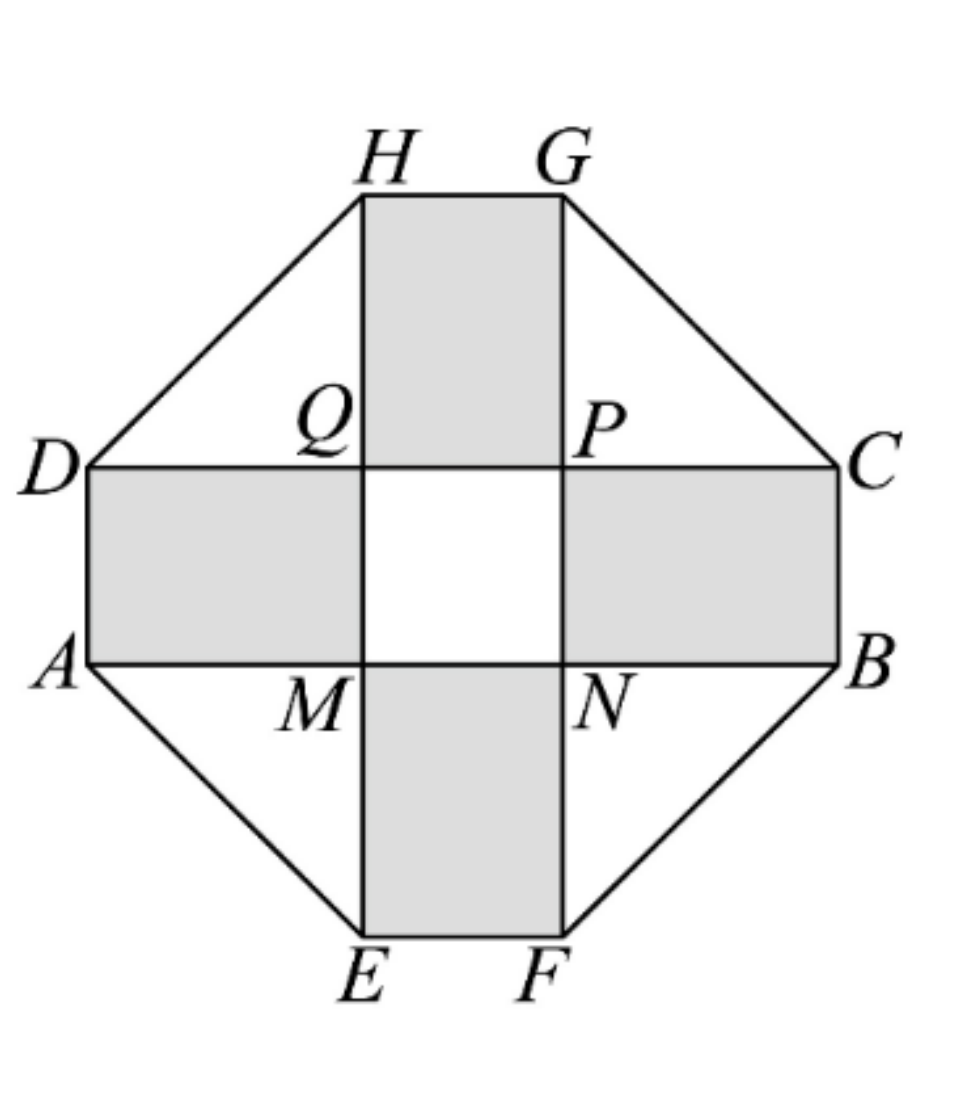
\includegraphics[width=0.34\textwidth]{figures/cross_octagon_h64.png}
\end{center}

\begin{enumerate}[label=(\arabic*)]
\item 设 $DQ$ 长为 $y\mathrm{m}$（$y>0$），用 $x$ 表示 $y$，并求出 $x$ 的取值范围；
\item 如何设计 $AD$ 可使总造价最低，并求出最低造价.
\item 若总造价 $W$ 不超过 69000 元，求 $AD$ 长 $x$ 的取值范围.
\end{enumerate}

\ifanswer
\solbegin
\stepm{(1)}{设 $DQ$ 长为 $y\mathrm{m}$，因为十字形区域面积为 $200\text{m}^2$，}
\step{所以 $4xy+x^2=200$，解得 $y=\dfrac{200-x^2}{4x}=\dfrac{50}{x}-\dfrac x4$；\dots\dots2 分}
\step{因为 $y>0$，所以 $x^2<200$，因为 $x>0$，所以 $0<x<10\sqrt2$.\dots\dots4 分}
\stepm{(2)}{四个矩形地砖面积 $S_{\text{四个矩形}}=4xy=200-x^2$，}
\step{造价 $W_{\text{四个矩形}}=105(200-x^2)$；}
\step{四个三角形草坪面积 $S_{\text{三角形}}=4\times\dfrac12y^2=2\left(\dfrac{50}{x}-\dfrac x4\right)^2=\dfrac{5000}{x^2}+\dfrac{x^2}8-50$，}
\step{造价 $W_{\text{三角形}}=40\left(\dfrac{5000}{x^2}+\dfrac{x^2}8-50\right)$；}
\step{正方形花坛面积 $S_{\text{正方形}}=x^2$，造价 $W_{\text{正方形}}=2100x^2$；}
\step{总造价 $W=W_{\text{四个矩形}}+W_{\text{三角形}}+W_{\text{正方形}}$}
\step{$=105(200-x^2)+40\left(\dfrac{5000}{x^2}+\dfrac{x^2}8-50\right)+2100x^2$，}
\step{化简得 $W=2000x^2+19000+\dfrac{200000}{x^2}$（$0<x<10\sqrt2$）.\dots\dots6 分}
\step{因为 $2000x^2+\dfrac{200000}{x^2}\geqslant40000$，}
\step{当且仅当 $x=\sqrt{10}$（在 $x$ 范围中）时取等号，此时 $W=59000$ 元.}
\step{综上，当 $AD$ 的长为 $\sqrt{10}$ 时，总造价最低，为 59000 元.\dots\dots8 分}
% 原卷 (3) 定义域印作 0<x<2√10，与 (1) 所得 0<x<10√2 不一致，照录（见文件头“原卷笔误”④）
\stepm{(3)}{由（2）得 $W=2000x^2+19000+\dfrac{200000}{x^2}$（$0<x<2\sqrt{10}$）.}
\step{总造价不超过 69000 元，即 $W=2000x^2+19000+\dfrac{200000}{x^2}\leqslant69000$，}
\step{化简得 $x^2+\dfrac{100}{x^2}\leqslant25$，\dots\dots10 分}
\step{即 $(x^2)^2-25x^2+100=(x^2-20)(x^2-5)\leqslant0$，即 $\sqrt5\leqslant x\leqslant2\sqrt5$，}
% 原卷末句“取值范围[√5,2√5]”脱“为”，照录（见文件头“原卷笔误”⑤）
\step{所以 $AD$ 长 $x$ 的取值范围$[\sqrt5,2\sqrt5]$.\dots\dots12 分}
\solend
\fi

\ansspace[10]

\item 设 $a,b,c$ 为实数，集合 $S=\{x\mid(x+a)(x^2+bx+c)=0,x\in\R\}$.

\begin{enumerate}[label=(\arabic*)]
\item 若 $a=1,b=3,c=2$，求集合 $S$；
\item 若 $S=\{-2\}$，求 $a,b,c$ 满足的条件；
\item 设 $T=\{x\mid(ax+1)(cx^2+bx+1)=0,x\in\R\}$，当 $ac\neq0$ 时，如果 $\dfrac12\in S$，$-2\in T$，且
集合 $S,T$ 均恰有两个元素，求三元数对 $(a,b,c)$.
\end{enumerate}

\ifanswer
\solbegin
\stepm{(1)}{若 $a=1,b=3,c=2$，}
\step{则方程 $(x+a)(x^2+bx+c)=0$ 为 $(x+1)(x^2+3x+2)=0$，}
\step{即 $(x+1)^2(x+2)=0$，解得 $x=-1$ 或 $x=-2$，所以 $S=\{-1,-2\}$；}
\stepm{(2)}{由题意得 $-a\in S$，因为 $S=\{-2\}$，所以 $-2$ 是方程 $x+a=0$ 的根，}
\step{即 $-2+a=0$，解得 $a=2$. 由 $S=\{-2\}$，集合 $S$ 有且仅有一个元素，}
\step{即方程 $(x+a)(x^2+bx+c)=0$ 有且仅有一个根，}
\stepm{①}{若 $-2$ 是方程 $x^2+bx+c=0$ 的根，}
\step{则 $\Delta=b^2-4c=0$，且 $-\dfrac b2=-2$，解得 $b=4,c=4$；}
\stepm{②}{若 $-2$ 不是方程 $x^2+bx+c=0$ 的根，则方程 $x^2+bx+c=0$ 无实数根，}
\step{则 $\Delta=b^2-4c<0$，}
\step{综上所述，$\begin{cases}a=2\\ b=4\\ c=4\end{cases}$ 或 $\begin{cases}a=2\\ b^2-4c<0\end{cases}$.}
\stepm{(3)}{$S=\{x\mid(x+a)(x^2+bx+c)=0,x\in\R\}$，}
\step{$T=\{x\mid(ax+1)(cx^2+bx+1)=0,x\in\R\}$，}
\step{由题意得 $a\neq0$ 且 $c\neq0$，则 $-a\in S,-\dfrac1a\in T$，}
\step{且方程 $x^2+bx+c=0$ 与 $cx^2+bx+1=0$ 有相同的判别式 $\Delta=b^2-4c$，}
\step{即两方程根的个数相同. 由集合 $S,T$ 均恰有两个元素，则 $\Delta=b^2-4c\geqslant0$.}
\step{$S=\{x\mid(x+a)(x^2+bx+c)=0,x\in\R\}$，}
\step{因为 $\dfrac12\in S$，所以 $\dfrac12$ 是方程 $x+a=0$ 或 $x^2+bx+c=0$ 的根.}
\step{$T=\{x\mid(ax+1)(cx^2+bx+1)=0,x\in\R\}$，}
\step{由 $-\dfrac1a\in T$，且 $-2\in T$，则 $-2$ 是方程 $ax+1=0$ 或 $cx^2+bx+1=0$ 的根.}
\stepm{①}{当 $a=-\dfrac12$ 时，$\dfrac12$ 是方程 $x+a=0$ 的根，$-a=\dfrac12\in S$，则 $-\dfrac1a=2\in T$，}
\step{又 $-2\in T$，则 $T=\{-2,2\}$，}
\step{由 $T=\left\{x\mid\left(-\dfrac12x+1\right)(cx^2+bx+1)=0,x\in\R\right\}$，}
% 原卷句末为句号，本稿原错作逗号
\step{则 $-2$ 是方程 $cx^2+bx+1=0$ 的根，则 $4c-2b+1=0$.}
\stepm{(i)}{若 $\Delta=b^2-4c=0$，联立 $\begin{cases}4c-2b+1=0\\ b^2-4c=0\end{cases}$ 解得 $b=1,c=\dfrac14$.}
\step{验证：当 $a=-\dfrac12,b=1,c=\dfrac14$ 时，}
\step{$S=\left\{x\mid\left(x-\dfrac12\right)\left(x^2+x+\dfrac14\right)=0,x\in\R\right\}=\left\{-\dfrac12,\dfrac12\right\}$，}
\step{$T=\left\{x\mid\left(-\dfrac12x+1\right)\left(\dfrac14x^2+x+1\right)=0,x\in\R\right\}=\{-2,2\}$，满足题意；}
\stepm{(ii)}{若 $\Delta=b^2-4c>0$，方程 $cx^2+bx+1=0$ 有两个不相等的实数根，}
\step{又 $T=\{-2,2\}$，则方程 $cx^2+bx+1=0$ 的两根必为 $-2$ 和 2.}
\step{由韦达定理得 $\begin{cases}-2+2=-\dfrac bc\\ -2\times2=\dfrac1c\end{cases}$，解得 $b=0,c=-\dfrac14$；}
\step{验证：当 $a=-\dfrac12,b=0,c=-\dfrac14$ 时，}
\step{$S=\left\{x\mid\left(x-\dfrac12\right)\left(x^2-\dfrac14\right)=0,x\in\R\right\}=\left\{-\dfrac12,\dfrac12\right\}$，}
\step{$T=\left\{x\mid\left(-\dfrac12x+1\right)\left(-\dfrac14x^2+1\right)=0,x\in\R\right\}=\{-2,2\}$，满足题意；}
\stepm{②}{当 $a=\dfrac12$ 时，$-\dfrac1a=-2$，即 $-2$ 是方程 $ax+1=0$ 的根，}
\step{则 $-a=-\dfrac12\in S$，又 $\dfrac12\in S$，则 $S=\left\{-\dfrac12,\dfrac12\right\}$，}
\step{$S=\{x\mid(x+a)(x^2+bx+c)=0,x\in\R\}$，}
\step{则 $\dfrac12$ 是方程 $x^2+bx+c=0$ 的根，则 $\dfrac14+\dfrac12b+c=0$，即 $4c+2b+1=0$；}
\stepm{(i)}{若 $\Delta=b^2-4c=0$，联立 $\begin{cases}4c+2b+1=0\\ b^2-4c=0\end{cases}$ 解得 $b=-1,c=\dfrac14$.}
\step{验证：当 $a=\dfrac12,b=-1,c=\dfrac14$ 时，}
\step{$S=\left\{x\mid\left(x+\dfrac12\right)\left(x^2-x+\dfrac14\right)=0,x\in\R\right\}=\left\{-\dfrac12,\dfrac12\right\}$，}
\step{$T=\left\{x\mid\left(\dfrac12x+1\right)\left(\dfrac14x^2-x+1\right)=0,x\in\R\right\}=\{-2,2\}$，满足题意；}
% 原卷作“有两不等的实数根”，本稿原脱“的”
\stepm{(ii)}{若 $\Delta=b^2-4c>0$，方程 $x^2+bx+c=0$ 有两不等的实数根，}
% 原卷句末为句号，本稿原错作逗号
\step{又 $S=\left\{-\dfrac12,\dfrac12\right\}$，则方程 $x^2+bx+c=0$ 的两根必为 $-\dfrac12$ 和 $\dfrac12$.}
\step{由韦达定理得 $\begin{cases}-\dfrac12+\dfrac12=-b\\ -\dfrac12\times\dfrac12=c\end{cases}$，解得 $b=0,c=-\dfrac14$；}
\step{验证：当 $a=\dfrac12,b=0,c=-\dfrac14$ 时，}
\step{$S=\left\{x\mid\left(x+\dfrac12\right)\left(x^2-\dfrac14\right)=0,x\in\R\right\}=\left\{-\dfrac12,\dfrac12\right\}$，}
\step{$T=\left\{x\mid\left(\dfrac12x+1\right)\left(-\dfrac14x^2+1\right)=0,x\in\R\right\}=\{-2,2\}$，满足题意；}
\stepm{③}{当 $a\neq-\dfrac12$ 且 $a\neq\dfrac12$ 时，则 $\dfrac12$ 不是方程 $x+a=0$ 的根，}
\step{$-2$ 也不是方程 $ax+1=0$ 的根.}
% 原卷此句单根而称“两实数根”，语病，照录（见文件头“原卷笔误”⑥）
\step{由 $\dfrac12\in S,-2\in T$，则 $\dfrac12$ 是方程 $x^2+bx+c=0$ 的两实数根，}
\step{且 $-2$ 是方程 $cx^2+bx+1=0$ 的根，则有 $\begin{cases}\dfrac14+\dfrac12b+c=0\\ 4c-2b+1=0\end{cases}$，}
\step{解得 $b=0,c=-\dfrac14$.}
\step{验证：当 $a\neq-\dfrac12$ 且 $a\neq\dfrac12,b=0,c=-\dfrac14$ 时，有 $-a\neq\dfrac12,-a\neq-\dfrac12$.}
\step{$S=\left\{x\mid(x+a)\left(x^2-\dfrac14\right)=0,x\in\R\right\}=\left\{-a,-\dfrac12,\dfrac12\right\}$ 有三个元素，}
\step{故不满足题意；}
\step{综上所述，满足题意的所有三元数对 $(a,b,c)$ 有}
\step{$\left(-\dfrac12,1,\dfrac14\right)$，$\left(-\dfrac12,0,-\dfrac14\right)$，$\left(\dfrac12,-1,\dfrac14\right)$，$\left(\dfrac12,0,-\dfrac14\right)$.}
\solend
\fi

\ansspace*[10]

\end{enumerate}

\end{document}
"
%
% 原始材料：微信公众号“魔都数学加油站”文章，作者破晓，连载“27学年高一64”；
% 原文标题“27学年高一64——2026-2027年上海市格致中学高一上10月月考”；
% 原文链接：https://mp.weixin.qq.com/s/0DfB77nTJf7NdVI_FYXxeA。
% 页面标注发布时间 2026-10-17 21:58（上海）。
% 本次转录只据 `原图/高一64_格致中学_10月月考/` 的 14 张 PNG 逐页读图。
% 正文为 14 张 PNG 页（`01..14.png`）：第 12、13、14 页 2560×3620，
% 第 01—11 页 4762×6735（**同一篇各页分辨率不同**），均按页序读取。
% 14 页全为试卷正文页（卷首标题在第 1 页页顶，卷末解答题第 18 题解析止于第 14 页），
% 无封面页、目录页、二维码或宣传页。粉色斜排“魔都数学加油站”为卷面水印，与公众号页脚一并未录入。
%
% 卷首标题：照卷面印作“2026--2027 年格致中学高一上 10 月月考”，年份区间按全稿惯例排 en dash。
% 原卷只有一行标题、无副标题。
%
% 篇幅与题号：原卷自第 3 题起编号（第 1、2 题不在本卷内）。填空题 3—10（8 题）、
% 选择题 11—14（4 题）、解答题 15—18（4 题），共 16 题。本稿沿用原节与原题号，
% 只改排为全稿统一的大节样式（原卷小节标题为“一、填空题”“二、选择题”“三、解答题”）。
%
% 讲评版：原卷每题下直接印【答案】或【解析】。**只印【答案】的 1 题**（第 5 题），
% 本稿只给 \ans{}；其余 15 题都印【解析】（按全稿口径这类题不另提 \ans{}——第 11、13、14 题
% 的结论写在解析末句（“故选 A”“故选 D”等），亦照录在解析内）。**另有 1 题答案印在题干括号内**——
% 第 12 题（“( B )”，该题无【答案】/【解析】段），本稿按 高一37 第 13 题成例把括号留空、
% 答案另提为 \ans{$B$}。
%
% 副标题：原卷未印副标题。本稿按“知识模块”口径标作“集合与常用逻辑用语、不等式”：
% 16 题中集合与常用逻辑用语 8 题（第 4、9、10、11、12、13、16、18 题），
% 不等式 8 题（含一元二次方程与韦达定理、基本不等式、二次不等式、恒成立、分式不等式：
% 第 3、5、6、7、8、14、15、17 题），两类均达三分之一，故并标。口径同 高一59、高一63。
%
% 与原卷的排版差异：
%   ① 原卷每题下直接印【答案】/【解析】，本稿按全稿惯例将答案与解析置于答案版，试卷版保持干净；
%   ② 原卷未印副标题，本稿按“知识模块”口径补出；
%   ③ 原卷填空横线约三四个字宽，本稿按全稿惯例统一排 \blankline[4.4em]；
%   ④ 原卷实数集排斜体 $R$（第 4、7、8、13、15、18 题）或粗体 $\mathbf{R}$（第 18 题题干与
%      解析共 6 处），整数集排斜体 $Z$（第 9、13 题）或粗体 $\mathbf{Z}$（第 9 题解析末两行），
%      有理数集排粗体 $\mathbf{Q}$（第 13 题选项 A），本稿按全稿惯例统一改用 $\R$、$\Z$、$\Q$
%      （记号归一，粗体／斜体不作区分）；空集记号原卷作 $\varnothing$，照录；
%   ⑤ 第 4 题的补集**原卷用上划线记号 $\bar B$**（题干 1 处、解析 4 处，共 5 处），
%      与全稿惯例的 $\complement_U B$ 不同，本稿照录原卷的 $\bar B$；
%   ⑥ 原卷用描述法时竖线排细竖“$|$”（如 $\{x\mid|x|\geqslant2024\}$ 一类），本稿按全稿惯例排 \mid；
%   ⑦ 第 15—18 题的子问原卷各自另起一行、以“（1）”“（2）”“（3）”标号，本稿按全稿惯例用
%      enumerate 的 (1)(2)(3)；解析中的子问标号一律用 \stepm{(1)}{…}；
%      第 18 题解析中分情形的①②③与分小目的 (i)(ii)，按全稿惯例作 \stepm{①}{…}、\stepm{(i)}{…}；
%   ⑧ 第 13 题解析的“A 选项：”“B 选项：”“C 选项：”“D 选项：”原卷排**加粗**（共 4 处），
%      同 高一63“法一：”成例，本稿排 \stepm{A 选项：}{…} 一类（加粗着色、不改黑色基调），
%      冒号照原卷排全角；
%   ⑨ 第 17 题解析带评分档，原卷在档与档之间排一串点线（“………2 分”），
%      本稿照录为“\dots\dots2 分”一类（同 高一54 成例），共 5 处；
%   ⑩ 选择题的作答括号原卷排半角“(　　)”（第 11、13、14 题括号内空白、第 12 题括号内印 B），
%      本稿按全稿惯例排 \mbox{（\quad）}；选项字母后的句点照原卷排“A.”“B.”；
%   ⑪ 每道解答题原卷未留作答空白，本稿按全稿惯例加 \ansspace（末题用 \ansspace*）；
%   ⑫ 第 17 题题干右侧的十字形八边形示意图，本稿按原卷截图裁出（`figures/cross_octagon_h64.png`，
%      原分辨率裁切，未放大、未用 TikZ 重绘），图内阴影与点名照原卷。
%
% 原卷笔误/存疑（均照录未改，正文对应处另有 % 注）：
%   ① 第 8 题解析末两步自相矛盾：上一步已化为 $\dfrac x{x-1}<0$，下一步却印作
%      “即 $x(x+1)<0$，解得 $-1<x<0$”并给出解集 $(-1,0)$——由 $\dfrac x{x-1}<0$ 应得
%      $x(x-1)<0$、解集 $(0,1)$；已 8 倍放大确认原卷确为 $x+1$ 与 $(-1,0)$，照录未改。
%   ② 第 13 题 D 选项解析“乘法满足结合率”的“率”应为“律”（同段 A、B 选项均作“结合律”）。
%   ③ 第 13 题条件①“任意 $a,b\in G$. 有 $a*b\in G$；”在 $G$ 后印句号（其余三条均以逗号
%      接下文），疑为逗号之误，照录。
%   ④ 第 17 题 (3) 解析把定义域印作 $0<x<2\sqrt{10}$，与 (1) 所得 $0<x<10\sqrt2$ 不一致
%      （疑为 $10\sqrt2$ 之误）；照录未改。
%   ⑤ 第 17 题 (3) 末句“所以 $AD$ 长 $x$ 的取值范围$[\sqrt5,2\sqrt5]$.”脱一个“为”。
%   ⑥ 第 18 题 (3) ③“则 $\dfrac12$ 是方程 $x^2+bx+c=0$ 的**两**实数根”——只有一个数却称
%      “两实数根”，语病；照录。
%
% 插图：第 17 题题干有 1 幅十字形八边形示意图（原卷第 09 页右侧），已按原卷截图排入；
% 其余 13 页无任何图形、无“如图”字样（第 17 题的“图中”均指此图）。
%
\documentclass[a4paper,11pt]{article}
\usepackage{common}

\begin{document}

\examtitlest[3]{2026--2027 年格致中学高一上 10 月月考}{集合与常用逻辑用语、不等式}

\bigsec{一、填空题}

\begin{enumerate}
\setcounter{enumi}{2}

\item 已知一元二次方程 $x^2-nx+5=0$ 的两个实根分别为 $x_1$、$x_2$，且 $\dfrac1{x_1}+\dfrac1{x_2}=1$，则实数 $n$ 的值为\blankline[4.4em].

\ifanswer
\solbegin
\step{$\dfrac1{x_1}+\dfrac1{x_2}=\dfrac{x_1+x_2}{x_1x_2}=\dfrac n5=1$，所以 $n=5$.}
\solend
\fi

\item 全集为 $U=\R$，$A=\{x\mid|x|\geqslant2\}$，$B=\{y\mid y=x^2+1,x\in\R\}$，则 $A\cup\bar B=$\blankline[4.4em].

\ifanswer
\solbegin
\step{由题意得集合 $A=\{x\mid x\geqslant2\text{ 或 }x\leqslant-2\}$，}
\step{因为 $x^2+1\geqslant1$，所以集合 $B=\{x\mid x\geqslant1\}$，所以 $\bar B=\{x\mid x<1\}$，}
\step{则 $A\cup\bar B=\{x\mid x\geqslant2\text{ 或 }x<1\}$.}
\solend
\fi

\item 若 $x>2$，则 $4x+\dfrac1{x-2}$ 的最小值为\blankline[4.4em].

\ifanswer
\ans{$12$}
\fi

\item 已知关于 $x$ 不等式组$\begin{cases}(3x-2)(2x+3)\leqslant0\\ x-a<0\end{cases}$\!没有实数解，则实数 $a$ 的取值范围为\blankline[4.4em].

\ifanswer
\solbegin
\step{由题意得 $\begin{cases}-\dfrac32\leqslant x\leqslant\dfrac23\\ x<a\end{cases}$ 无解，所以 $a\leqslant-\dfrac32$.}
\solend
\fi

\item 若不等式 $\dfrac{x^2-8x+20}{mx^2-mx-1}<0$ 对一切 $x\in\R$ 都成立，则实数 $m$ 的取值范围为\blankline[4.4em].

\ifanswer
\solbegin
\step{因为 $x^2-8x+20=(x-4)^2+4\geqslant4>0$，所以 $mx^2-mx-1<0$，}
\step{当 $m=0$ 时，$mx^2-mx-1=-1<0$，不等式成立；}
\step{设 $y=mx^2-mx-1$，当 $m\neq0$ 时函数 $y$ 为二次函数，$y$ 要恒小于 0，}
\step{抛物线开口向下且与 $x$ 轴没有交点，即 $m<0$ 且 $\Delta<0$，得 $-4<m\leqslant0$，}
\step{故实数 $m$ 的取值范围为 $(-4,0]$.}
\solend
\fi

\item 已知关于 $x$ 的不等式 $\dfrac{ax-1}{x+b}>0$ 的解集为 $\{x\mid-1<x<2\}$，其中 $a$、$b\in\R$，则关于 $x$ 的不等式 $\dfrac{bx+1}{ax+1}<1$ 的解集为\blankline[4.4em].

\ifanswer
\solbegin
\step{不等式 $\dfrac{ax-1}{x+b}>0$ 等价于 $(ax-1)(x+b)>0$，即 $ax^2+(ab-1)x-b>0$，}
\step{所以 $-1$ 和 2 为方程 $ax^2+(ab-1)x-b=0$ 的两根，且 $a<0$，}
\step{由韦达定理得 $\begin{cases}-1+2=-\dfrac{ab-1}a\\ -1\times2=-\dfrac ba\end{cases}$，解得 $\begin{cases}a=-1\\ b=-2\end{cases}$，}
\step{所以原不等式为 $\dfrac{-2x+1}{-x+1}<1\Rightarrow\dfrac{-2x+1}{-x+1}-1<0\Rightarrow\dfrac{-x}{-x+1}<0\Rightarrow\dfrac x{x-1}<0$，}
% 原卷下一步印作“即 x(x+1)<0，解得 -1<x<0”，与上一步 x/(x-1)<0 不等价，
% 照录未改（见文件头“原卷笔误”①）
\step{即 $x(x+1)<0$，解得 $-1<x<0$，即不等式 $\dfrac{bx+1}{ax+1}<1$ 的解集为 $(-1,0)$.}
\solend
\fi

\item 已知集合 $M=\{x\mid|x|\leqslant2024,x\in\Z\}$，集合 $P$ 是 $M$ 的三元子集，即 $P=\{a,b,c\}\subseteq M$，$P$~中元素 $a,b,c$ 满足 $\begin{cases}\dfrac1a+\dfrac1b=\dfrac2c\\ a+c=2b\end{cases}$，则符合要求的集合 $P$ 有\blankline[4.4em]个.

\ifanswer
\solbegin
\step{由 $a+c=2b$，则 $a=2b-c$，代入 $\dfrac1a+\dfrac1b=\dfrac2c$，即 $\dfrac1{2b-c}=\dfrac2c-\dfrac1b=\dfrac{2b-c}{bc}$，}
\step{整理得 $(2b-c)^2=bc$，展开得 $4b^2-5bc+c^2=0$，}
\step{解得 $b=\dfrac c4$ 或 $b=c$（由集合的互异性，舍去），代入 $a+c=2b$ 得 $a=-\dfrac c2$，}
\step{则 $P=\left\{-\dfrac c2,\dfrac c4,c\right\}\subseteq\{x\mid-2024\leqslant x\leqslant2024,x\in\Z\}$，所以 $c$ 为 4 的整数倍，}
\step{且不为 0，则共有 $\dfrac{2024}4\times2=1012$ 个.}
\solend
\fi

\item 已知正整数 $n\geqslant2$，对集合 $\{1,2,3,\cdots,n\}$ 及其每一个非空子集 $X$，记
$X=\{x_1,x_2,\cdots,x_k\}$，其中 $x_1>x_2>\cdots>x_k$，定义一个运算“交替和”
$S_X=x_1-x_2+x_3\cdots+(-1)^{k+1}x_k$. 例如：对于集合 $X=\{9,6,4,2,1\}$，
$S_X=9-6+4-2+1=6$. 则当 $n=7$ 时，集合 $\{1,2,3,\cdots,n\}$ 的所有子集的“交替和”的总
和为\blankline[4.4em].

\ifanswer
\solbegin
\step{由题意得集合 $\{7\}$ 的“交替和”为 7.}
\step{集合 $\{1,2,3,4,5,6,7\}$ 的所有 $2^7$ 个子集中，除去集合 $\{7\}$ 外，}
\step{还有 $2^7-2$ 个非空子集，这 $2^7-2$ 个非空子集中不含元素 7 的集合，}
\step{即 $\{1,2,3,4,5,6\}$ 的非空子集，共有 $2^6-1$ 个，设为 $A_i(i=1,2,\cdots,2^6-1)$；}
\step{则这 $2^7-2$ 个非空子集中含元素 7 的集合，也共有 $2^6-1$ 个，}
\step{这样的集合都可以看成相应地在每个不含 7 的集合中再加上元素 7 得到，}
\step{即 $A_i\cup\{7\}$.}
\step{对 $A_i(i=1,2,\cdots,2^6-1)$ 中的任意集合 $A$，记 $A=\{x_1,x_2,\cdots,x_k\}$，}
\step{则“交替和”$S_A=x_1-x_2+x_3\cdots+(-1)^{k+1}x_k$，其中 $x_1>x_2>\cdots>x_k$，}
\step{由 $7>x_1>x_2>\cdots>x_k$，}
\step{则集合 $A\cup\{7\}$ 的“交替和”为 $7-[x_1-x_2+x_3\cdots+(-1)^{k+1}x_k]$，}
\step{则集合 $A$ 与集合 $A\cup\{7\}$ 的“交替和”之和为 7，下面举例说明：}
\step{如集合 $\{6,5,4,3,2,1\}$ 与集合 $\{7,6,5,4,3,2,1\}$，}
\step{$\{6,5,4,3,2,1\}$ 的“交替和”为 $6-5+4-3+2-1=3$，}
% 原卷此句在页末折为两个印刷行（“……的“交替和”为”／“7-6+5-4+3-2+1=……”），
% 本稿原并作一条，现照原卷拆开（原卷原样两行 / 本稿原错处：并作一行）
\step{$\{7,6,5,4,3,2,1\}$ 的“交替和”为}
\step{$7-6+5-4+3-2+1=7-(6-5+4-3+2-1)=7-3$，}
\step{即集合 $\{6,5,4,3,2,1\}$ 与集合 $\{7,6,5,4,3,2,1\}$ 的“交替和”之和为 7.}
\step{综上，把这 $2^7-2$ 个非空子集两两结组后分别计算每一组中“交替和”之和，}
\step{且每组中“交替和”之和都为 7，共有 $2^6-1$ 组.}
\step{故集合 $\{1,2,3,4,5,6,7\}$ 所有“交替和”之和，}
\step{由各组之和再加集合 $\{7\}$ 的“交替和”7 即可，}
\step{综上所述，当 $n=7$ 时，集合 $\{1,2,3,\cdots,n\}$ 的所有子集的所有“交替和”之和}
\step{为 $7\times(2^6-1)+7=448$.}
\solend
\fi

\end{enumerate}

\bigsec{二、选择题}

\begin{enumerate}
\setcounter{enumi}{10}

\item 若 $a$、$b\in\R$，则“$a<b<0$”是“$a^2>b^2$”的\mbox{（\quad）}条件.

\keepwithprev
A. 充分非必要\qquad B. 必要非充分

C. 充要\qquad D. 既非充分也非必要

\ifanswer
\solbegin
\step{由 $a<b<0\Rightarrow-a>-b>0\Rightarrow(-a)^2>(-b)^2\Rightarrow a^2>b^2$，}
\step{因此由 $a<b<0$ 可以推出 $a^2>b^2$，}
\step{但是当 $a=1$，$b=0$ 时，显然 $a^2>b^2$ 成立，但是 $a<b<0$ 不成立，}
\step{因此由 $a^2>b^2$ 不一定能推出 $a<b<0$，}
\step{因此“$a<b<0$”是“$a^2>b^2$”的充分非必要条件. 故选 $A$.}
\solend
\fi

% 第 12 题答案“B”直接印在题干括号内“(  B  )”，且该题无【答案】/【解析】段；
% 按 高一37 第 13 题的成例括号留空、答案另提为 \ans{}（见文件头）
\item 用反证法证明结论“$a$、$b$、$c$ 至少有一个是正数”时，应假设\mbox{（\quad）}

\keepwithprev
A. $a$、$b$、$c$ 都是正数\qquad B. $a$、$b$、$c$ 都不是正数

C. $a$、$b$、$c$ 至多有一个正数\qquad D. $a$、$b$、$c$ 至多有两个正数

\ifanswer
\ans{$B$}
\fi

\item “群”的概念由数学家伽罗瓦在 19 世纪 30 年代开创，群论虽起源于对代数多项式方程
的研究，但在量子力学、晶体结构学等其他学科中也有十分广泛的应用.“群”的定义是：

设 $G$ 为某种元素组成的一个非空集合，若在 $G$ 内定义一个运算“*”，满足以下条件：

% 原卷条件①在 G 后印句号，疑为逗号之误，照录（见文件头“原卷笔误”③）
①任意 $a,b\in G$. 有 $a*b\in G$；

②如 $a,b,c\in G$，有 $(a*b)*c=a*(b*c)$；

③在 $G$ 中有一个元素 $e$，对任意 $a\in G$，都有 $a*e=e*a=a$，称 $e$ 为 $G$ 的单位元；

④任意 $a\in G$，在 $G$ 中存在唯一确定的 $b$，使 $a*b=b*a=e$，称 $b$ 为 $a$ 的逆元；

此时称 $(G,*)$ 为一个群.

例如实数集 $\R$ 和实数集上的加法运算“+”就构成一个群 $(\R,+)$，其单位元是 0，每一个数
的逆元是其相反数，那么下列说法中，错误的是\mbox{（\quad）}

\keepwithprev
A. $G=\Q$，则 $(G,+)$ 为一个群

B. $G=\{\sqrt2m+\sqrt3n\mid m,n\in\Z\}$，$(G,+)$ 为一个群

C. $G=\{-1,1\}$，则 $(G,\times)$ 为一个群

D. $G=\{x\mid x=2k+1,k\in\Z\}$，则 $(G,\times)$ 为一个群

\ifanswer
\solbegin
\stepm{A 选项：}{有理数的和还是有理数，求和满足结合律，}
\step{设 $a\in\Q$，单位元为 $e$，则 $a+e=a$，故 $e=0$，}
\step{所以每一个数的相反数为其逆元，故 $(G,+)$ 为一个群，选项 A 正确；}
\stepm{B 选项：}{$G=\{\sqrt2m+\sqrt3n\mid m,n\in\Z\}$ 中的任何两个数相加还是属于}
\step{$G=\{\sqrt2m+\sqrt3n\mid m,n\in\Z\}$，求和满足结合律，}
\step{设 $\sqrt2x+\sqrt3y\in G,x,y\in\Z$，单位元为 $e$，}
\step{则 $\sqrt2x+\sqrt3y+e=\sqrt2x+\sqrt3y$，所以 $e=0$，}
\step{每一个数的相反数为其逆元，$(G,+)$ 为一个群，选项 B 正确；}
\stepm{C 选项：}{$G=\{-1,1\}$ 中的两个元素相乘，其积可能为 1 或 $-1$，又 $1\in G,-1\in G$，}
\step{设 $a\in G$，单位元为 $e$，则 $a\times e=a$，故 $e=1,1$ 的逆元为 $1,-1$ 的逆元为 $-1$，}
\step{所以 $(G,\times)$ 为一个群，选项 C 正确；}
% 原卷“乘法满足结合率”的“率”应为“律”（同段 A、B 选项均作“结合律”），照录（见文件头“原卷笔误”②）
\stepm{D 选项：}{两个奇数相乘还是奇数，乘法满足结合率，}
\step{设 $a\in G$，单位元为 $e$，则 $a\times e=a$，故 $e=1$，}
\step{又 $3\in G$，故存在 $b\in G$，使得 $3b=1$，则 $b=\dfrac13$，矛盾，}
\step{故 $(G,\times)$ 不为一个群，选项 D 错误.}
\step{故选 $D$.}
\solend
\fi

\item 已知 $a$、$b$、$c\in\R$，若关于 $x$ 的不等式 $0\leqslant x+\dfrac ax+b\leqslant\dfrac cx-1$ 的解集为 $[x_1,x_2]\cup\{x_3\}$
（$x_3>x_2>x_1>0$），则\mbox{（\quad）}

\keepwithprev
A. 不存在有序数组 $(a,b,c)$，使得 $x_2-x_1=1$

B. 存在唯一有序数组 $(a,b,c)$，使得 $x_2-x_1=1$

C. 有且只有两组有序数组 $(a,b,c)$，使得 $x_2-x_1=1$

D. 存在无穷多组有序数组 $(a,b,c)$，使得 $x_2-x_1=1$

\ifanswer
\solbegin
\step{因为不等式 $0\leqslant x+\dfrac ax+b\leqslant\dfrac cx-1$ 的解集为 $[x_1,x_2]\cup\{x_3\}$（$x_3>x_2>x_1>0$），}
\step{所以 $0\leqslant x^2+bx+a\leqslant c-x$ 在 $[x_1,x_2]\cup\{x_3\}$ 上成立，}
\step{假设 $x_1=m$，$x_2=m+1$，$x_3=n$，}
\step{则 $c-n=0=n^2+bn+a$，由 $x_3$ 为一个独立的数得出，}
\step{所以 $n=c$，且 $m+1$ 与 $n$ 为方程 $x^2+bx+a=0$ 的两个根，}
\step{因为 $x_3>x_2>x_1>0$，所以 $-b=m+n+1=m+c+1$，$a=mn+n=mc+c$，}
\step{所以 $b=-m-c-1$，}
\step{且点 $(x_1,x_1^2+bx_1+a)$ 为 $y=x^2+bx+a$ 与 $y=c-x$ 的左交点，}
\step{所以 $m^2+bm+a=c-m$ 且 $b=-m-c-1$，$a=mc+c$，}
\step{故 $m^2+bm+a=m^2-m^2-mc-m+mc+c=c-m$，所以 $c-m=c-m$ 恒成立，}
\step{所以不论 $a$、$b$、$c$ 取何值，$x_2-x_1=1$ 恒成立，}
\step{即存在无穷多组有序数组 $(a,b,c)$，使得 $x_2-x_1=1$，}
\step{故选项 $A$、$B$、$C$ 错误，选项 $D$ 正确. 故选 $D$.}
\solend
\fi

\end{enumerate}

\bigsec{三、解答题}

\begin{enumerate}
\setcounter{enumi}{14}

\item 已知函数 $f(x)=(a-1)x^2-ax+1$，$a\in\R$.

\begin{enumerate}[label=(\arabic*)]
\item 若不等式 $f(x)<0$ 的解集为 $\left(\dfrac13,1\right)$，求实数 $a$ 的值；
\item 当 $a>1$ 时，解关于 $x$ 的不等式 $f(x)\geqslant0$.
\end{enumerate}

\ifanswer
\solbegin
\stepm{(1)}{因为不等式 $f(x)<0$ 的解集为 $\left(\dfrac13,1\right)$，}
\step{所以不等式对应的方程 $(a-1)x^2-ax+1=0$ 的两根分别为 $\dfrac13$、1，}
\step{由根与系数的关系得 $\begin{cases}1+\dfrac13=\dfrac a{a-1}\\ 1\times\dfrac13=\dfrac1{a-1}\end{cases}$，解得 $a=4$；}
\stepm{(2)}{不等式 $(a-1)x^2-ax+1\geqslant0$（$a>1$）可化为 $(x-1)[(a-1)x-1]\geqslant0$，}
\step{不等式对应方程的两根为 $x_1=1$，$x_2=\dfrac1{a-1}$，}
\step{①当 $\dfrac1{a-1}=1$，即 $a=2$ 时，不等式为 $(x-1)^2\geqslant0$，解集为 $\R$；}
\step{②当 $\dfrac1{a-1}>1$，即 $1<a<2$ 时，解不等式得 $x\leqslant1$ 或 $x\geqslant\dfrac1{a-1}$；}
\step{③当 $\dfrac1{a-1}<1$，即 $a>2$ 时，解不等式得 $x\leqslant\dfrac1{a-1}$ 或 $x\geqslant1$；}
\step{综上，$a=2$ 时，不等式的解集为 $\R$，}
\step{$1<a<2$ 时，不等式的解集为 $(-\infty,1]\cup\left[\dfrac1{a-1},+\infty\right)$，}
\step{$a>2$ 时，不等式的解集为 $\left(-\infty,\dfrac1{a-1}\right]\cup[1,+\infty)$.}
\solend
\fi

\ansspace[6]

\item 若集合 $A=\{x\mid x^2+5x-6=0\}$，$B=\{x\mid x^2+2(m+1)x+m^2-3=0\}$.

\begin{enumerate}[label=(\arabic*)]
\item 若 $m=0$，写出 $A\cup B$ 的子集个数；
\item 若 $A\cap B=B$，求实数 $m$ 的取值范围.
\end{enumerate}

\ifanswer
\solbegin
\stepm{(1)}{当 $m=0$ 时，$B=\{1,-3\}$，}
\step{因为 $A=\{x\mid x^2+5x-6=0\}=\{-6,1\}$，}
\step{所以 $A\cup B=\{-6,-3,1\}$，集合元素个数为 3 个，}
\step{故 $A\cup B$ 的子集个数为 $2^3=8$.}
\stepm{(2)}{因为 $A\cap B=B$，所以 $B\subseteq A$，}
\step{$\Delta=4(m+1)^2-4(m^2-3)=8m+16$，}
\step{当 $\Delta<0$，即 $m<-2$ 时，$B=\varnothing$，符合题意，}
\step{当 $\Delta=0$，即 $m=-2$ 时，$B=\{1\}$，符合题意，}
\step{当 $\Delta>0$，即 $m>-2$ 时，若 $B\subseteq A$，则 $B=\{-6,1\}$，}
\step{即 $\begin{cases}-2(m+1)=-5\\ m^2-3=-6\end{cases}$，方程组无解，}
\step{综上所述，$m$ 的取值范围为 $(-\infty,-2]$.}
\solend
\fi

\ansspace[6]

\item 2025 年上海奇迹花园国际艺术花展于 9 月 20 日正式启幕，本次花展首次实现沉浸 IP
展、花卉景观、跨界艺术、光影夜花园四展合一，为市民游客打造一个可游、可赏、可感
的秋季治愈系童话世界. 某公园受此启发打算设计一个八边形活动区域，该区域的主体造
型平面图是由两个相同的矩形 $ABCD$ 和 $EFGH$ 构成的十字形地域，十字形的面积为
$200\text{m}^2$. 计划在正方形 $MNPQ$ 上建一座花坛，造价为 2100 元$/\text{m}^2$；在四个相同的矩形
（图中阴影部分）上铺地砖，造价为 105 元$/\text{m}^2$；再在四个空角（图中四个三角
形）上铺草坪，造价为 40 元$/\text{m}^2$. 设 $AD$ 长为 $x\mathrm{m}$（$x>0$），总造价为 $W$ 元，求：

\begin{center}
% 插图取自原卷第 09 页右侧截图（原分辨率裁切，未用 TikZ 重绘），阴影与点名照原卷
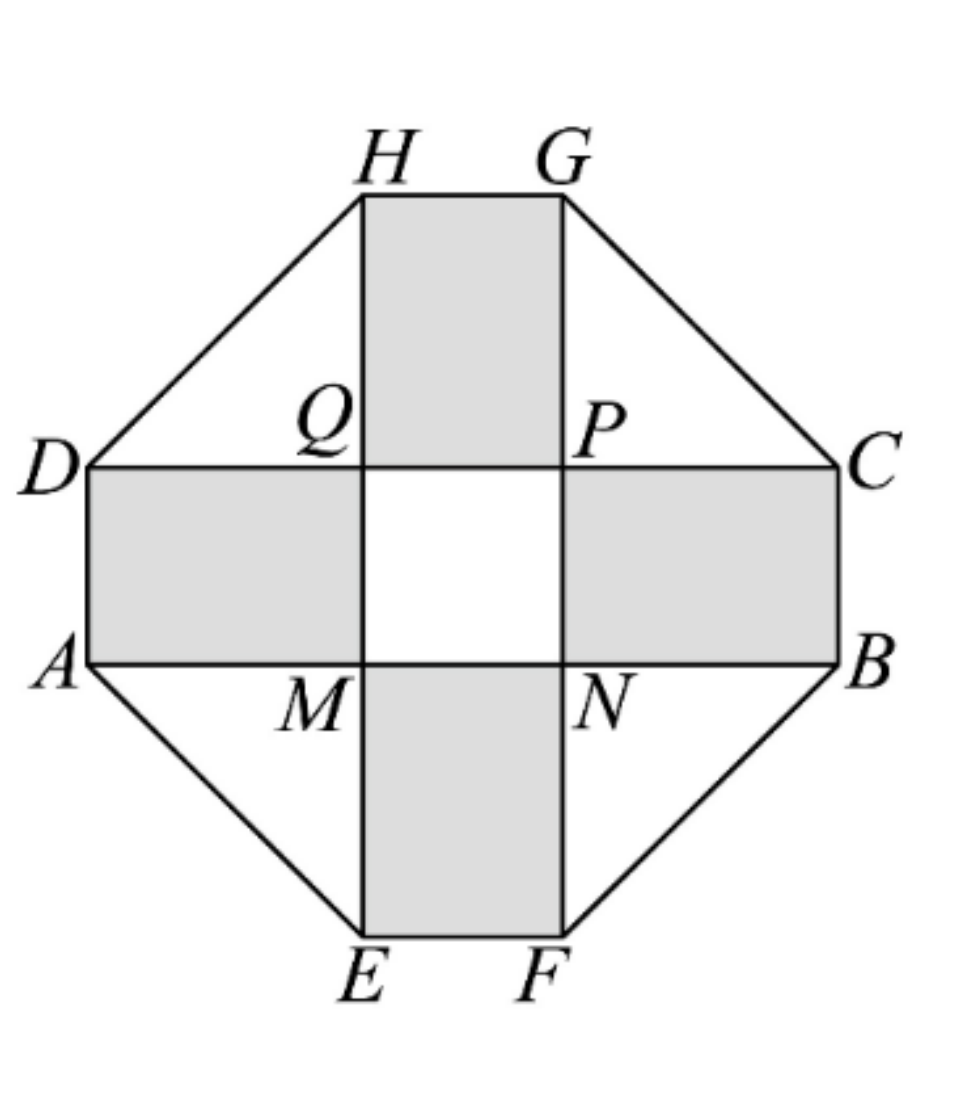
\includegraphics[width=0.34\textwidth]{figures/cross_octagon_h64.png}
\end{center}

\begin{enumerate}[label=(\arabic*)]
\item 设 $DQ$ 长为 $y\mathrm{m}$（$y>0$），用 $x$ 表示 $y$，并求出 $x$ 的取值范围；
\item 如何设计 $AD$ 可使总造价最低，并求出最低造价.
\item 若总造价 $W$ 不超过 69000 元，求 $AD$ 长 $x$ 的取值范围.
\end{enumerate}

\ifanswer
\solbegin
\stepm{(1)}{设 $DQ$ 长为 $y\mathrm{m}$，因为十字形区域面积为 $200\text{m}^2$，}
\step{所以 $4xy+x^2=200$，解得 $y=\dfrac{200-x^2}{4x}=\dfrac{50}{x}-\dfrac x4$；\dots\dots2 分}
\step{因为 $y>0$，所以 $x^2<200$，因为 $x>0$，所以 $0<x<10\sqrt2$.\dots\dots4 分}
\stepm{(2)}{四个矩形地砖面积 $S_{\text{四个矩形}}=4xy=200-x^2$，}
\step{造价 $W_{\text{四个矩形}}=105(200-x^2)$；}
\step{四个三角形草坪面积 $S_{\text{三角形}}=4\times\dfrac12y^2=2\left(\dfrac{50}{x}-\dfrac x4\right)^2=\dfrac{5000}{x^2}+\dfrac{x^2}8-50$，}
\step{造价 $W_{\text{三角形}}=40\left(\dfrac{5000}{x^2}+\dfrac{x^2}8-50\right)$；}
\step{正方形花坛面积 $S_{\text{正方形}}=x^2$，造价 $W_{\text{正方形}}=2100x^2$；}
\step{总造价 $W=W_{\text{四个矩形}}+W_{\text{三角形}}+W_{\text{正方形}}$}
\step{$=105(200-x^2)+40\left(\dfrac{5000}{x^2}+\dfrac{x^2}8-50\right)+2100x^2$，}
\step{化简得 $W=2000x^2+19000+\dfrac{200000}{x^2}$（$0<x<10\sqrt2$）.\dots\dots6 分}
\step{因为 $2000x^2+\dfrac{200000}{x^2}\geqslant40000$，}
\step{当且仅当 $x=\sqrt{10}$（在 $x$ 范围中）时取等号，此时 $W=59000$ 元.}
\step{综上，当 $AD$ 的长为 $\sqrt{10}$ 时，总造价最低，为 59000 元.\dots\dots8 分}
% 原卷 (3) 定义域印作 0<x<2√10，与 (1) 所得 0<x<10√2 不一致，照录（见文件头“原卷笔误”④）
\stepm{(3)}{由（2）得 $W=2000x^2+19000+\dfrac{200000}{x^2}$（$0<x<2\sqrt{10}$）.}
\step{总造价不超过 69000 元，即 $W=2000x^2+19000+\dfrac{200000}{x^2}\leqslant69000$，}
\step{化简得 $x^2+\dfrac{100}{x^2}\leqslant25$，\dots\dots10 分}
\step{即 $(x^2)^2-25x^2+100=(x^2-20)(x^2-5)\leqslant0$，即 $\sqrt5\leqslant x\leqslant2\sqrt5$，}
% 原卷末句“取值范围[√5,2√5]”脱“为”，照录（见文件头“原卷笔误”⑤）
\step{所以 $AD$ 长 $x$ 的取值范围$[\sqrt5,2\sqrt5]$.\dots\dots12 分}
\solend
\fi

\ansspace[10]

\item 设 $a,b,c$ 为实数，集合 $S=\{x\mid(x+a)(x^2+bx+c)=0,x\in\R\}$.

\begin{enumerate}[label=(\arabic*)]
\item 若 $a=1,b=3,c=2$，求集合 $S$；
\item 若 $S=\{-2\}$，求 $a,b,c$ 满足的条件；
\item 设 $T=\{x\mid(ax+1)(cx^2+bx+1)=0,x\in\R\}$，当 $ac\neq0$ 时，如果 $\dfrac12\in S$，$-2\in T$，且
集合 $S,T$ 均恰有两个元素，求三元数对 $(a,b,c)$.
\end{enumerate}

\ifanswer
\solbegin
\stepm{(1)}{若 $a=1,b=3,c=2$，}
\step{则方程 $(x+a)(x^2+bx+c)=0$ 为 $(x+1)(x^2+3x+2)=0$，}
\step{即 $(x+1)^2(x+2)=0$，解得 $x=-1$ 或 $x=-2$，所以 $S=\{-1,-2\}$；}
\stepm{(2)}{由题意得 $-a\in S$，因为 $S=\{-2\}$，所以 $-2$ 是方程 $x+a=0$ 的根，}
\step{即 $-2+a=0$，解得 $a=2$. 由 $S=\{-2\}$，集合 $S$ 有且仅有一个元素，}
\step{即方程 $(x+a)(x^2+bx+c)=0$ 有且仅有一个根，}
\stepm{①}{若 $-2$ 是方程 $x^2+bx+c=0$ 的根，}
\step{则 $\Delta=b^2-4c=0$，且 $-\dfrac b2=-2$，解得 $b=4,c=4$；}
\stepm{②}{若 $-2$ 不是方程 $x^2+bx+c=0$ 的根，则方程 $x^2+bx+c=0$ 无实数根，}
\step{则 $\Delta=b^2-4c<0$，}
\step{综上所述，$\begin{cases}a=2\\ b=4\\ c=4\end{cases}$ 或 $\begin{cases}a=2\\ b^2-4c<0\end{cases}$.}
\stepm{(3)}{$S=\{x\mid(x+a)(x^2+bx+c)=0,x\in\R\}$，}
\step{$T=\{x\mid(ax+1)(cx^2+bx+1)=0,x\in\R\}$，}
\step{由题意得 $a\neq0$ 且 $c\neq0$，则 $-a\in S,-\dfrac1a\in T$，}
\step{且方程 $x^2+bx+c=0$ 与 $cx^2+bx+1=0$ 有相同的判别式 $\Delta=b^2-4c$，}
\step{即两方程根的个数相同. 由集合 $S,T$ 均恰有两个元素，则 $\Delta=b^2-4c\geqslant0$.}
\step{$S=\{x\mid(x+a)(x^2+bx+c)=0,x\in\R\}$，}
\step{因为 $\dfrac12\in S$，所以 $\dfrac12$ 是方程 $x+a=0$ 或 $x^2+bx+c=0$ 的根.}
\step{$T=\{x\mid(ax+1)(cx^2+bx+1)=0,x\in\R\}$，}
\step{由 $-\dfrac1a\in T$，且 $-2\in T$，则 $-2$ 是方程 $ax+1=0$ 或 $cx^2+bx+1=0$ 的根.}
\stepm{①}{当 $a=-\dfrac12$ 时，$\dfrac12$ 是方程 $x+a=0$ 的根，$-a=\dfrac12\in S$，则 $-\dfrac1a=2\in T$，}
\step{又 $-2\in T$，则 $T=\{-2,2\}$，}
\step{由 $T=\left\{x\mid\left(-\dfrac12x+1\right)(cx^2+bx+1)=0,x\in\R\right\}$，}
% 原卷句末为句号，本稿原错作逗号
\step{则 $-2$ 是方程 $cx^2+bx+1=0$ 的根，则 $4c-2b+1=0$.}
\stepm{(i)}{若 $\Delta=b^2-4c=0$，联立 $\begin{cases}4c-2b+1=0\\ b^2-4c=0\end{cases}$ 解得 $b=1,c=\dfrac14$.}
\step{验证：当 $a=-\dfrac12,b=1,c=\dfrac14$ 时，}
\step{$S=\left\{x\mid\left(x-\dfrac12\right)\left(x^2+x+\dfrac14\right)=0,x\in\R\right\}=\left\{-\dfrac12,\dfrac12\right\}$，}
\step{$T=\left\{x\mid\left(-\dfrac12x+1\right)\left(\dfrac14x^2+x+1\right)=0,x\in\R\right\}=\{-2,2\}$，满足题意；}
\stepm{(ii)}{若 $\Delta=b^2-4c>0$，方程 $cx^2+bx+1=0$ 有两个不相等的实数根，}
\step{又 $T=\{-2,2\}$，则方程 $cx^2+bx+1=0$ 的两根必为 $-2$ 和 2.}
\step{由韦达定理得 $\begin{cases}-2+2=-\dfrac bc\\ -2\times2=\dfrac1c\end{cases}$，解得 $b=0,c=-\dfrac14$；}
\step{验证：当 $a=-\dfrac12,b=0,c=-\dfrac14$ 时，}
\step{$S=\left\{x\mid\left(x-\dfrac12\right)\left(x^2-\dfrac14\right)=0,x\in\R\right\}=\left\{-\dfrac12,\dfrac12\right\}$，}
\step{$T=\left\{x\mid\left(-\dfrac12x+1\right)\left(-\dfrac14x^2+1\right)=0,x\in\R\right\}=\{-2,2\}$，满足题意；}
\stepm{②}{当 $a=\dfrac12$ 时，$-\dfrac1a=-2$，即 $-2$ 是方程 $ax+1=0$ 的根，}
\step{则 $-a=-\dfrac12\in S$，又 $\dfrac12\in S$，则 $S=\left\{-\dfrac12,\dfrac12\right\}$，}
\step{$S=\{x\mid(x+a)(x^2+bx+c)=0,x\in\R\}$，}
\step{则 $\dfrac12$ 是方程 $x^2+bx+c=0$ 的根，则 $\dfrac14+\dfrac12b+c=0$，即 $4c+2b+1=0$；}
\stepm{(i)}{若 $\Delta=b^2-4c=0$，联立 $\begin{cases}4c+2b+1=0\\ b^2-4c=0\end{cases}$ 解得 $b=-1,c=\dfrac14$.}
\step{验证：当 $a=\dfrac12,b=-1,c=\dfrac14$ 时，}
\step{$S=\left\{x\mid\left(x+\dfrac12\right)\left(x^2-x+\dfrac14\right)=0,x\in\R\right\}=\left\{-\dfrac12,\dfrac12\right\}$，}
\step{$T=\left\{x\mid\left(\dfrac12x+1\right)\left(\dfrac14x^2-x+1\right)=0,x\in\R\right\}=\{-2,2\}$，满足题意；}
% 原卷作“有两不等的实数根”，本稿原脱“的”
\stepm{(ii)}{若 $\Delta=b^2-4c>0$，方程 $x^2+bx+c=0$ 有两不等的实数根，}
% 原卷句末为句号，本稿原错作逗号
\step{又 $S=\left\{-\dfrac12,\dfrac12\right\}$，则方程 $x^2+bx+c=0$ 的两根必为 $-\dfrac12$ 和 $\dfrac12$.}
\step{由韦达定理得 $\begin{cases}-\dfrac12+\dfrac12=-b\\ -\dfrac12\times\dfrac12=c\end{cases}$，解得 $b=0,c=-\dfrac14$；}
\step{验证：当 $a=\dfrac12,b=0,c=-\dfrac14$ 时，}
\step{$S=\left\{x\mid\left(x+\dfrac12\right)\left(x^2-\dfrac14\right)=0,x\in\R\right\}=\left\{-\dfrac12,\dfrac12\right\}$，}
\step{$T=\left\{x\mid\left(\dfrac12x+1\right)\left(-\dfrac14x^2+1\right)=0,x\in\R\right\}=\{-2,2\}$，满足题意；}
\stepm{③}{当 $a\neq-\dfrac12$ 且 $a\neq\dfrac12$ 时，则 $\dfrac12$ 不是方程 $x+a=0$ 的根，}
\step{$-2$ 也不是方程 $ax+1=0$ 的根.}
% 原卷此句单根而称“两实数根”，语病，照录（见文件头“原卷笔误”⑥）
\step{由 $\dfrac12\in S,-2\in T$，则 $\dfrac12$ 是方程 $x^2+bx+c=0$ 的两实数根，}
\step{且 $-2$ 是方程 $cx^2+bx+1=0$ 的根，则有 $\begin{cases}\dfrac14+\dfrac12b+c=0\\ 4c-2b+1=0\end{cases}$，}
\step{解得 $b=0,c=-\dfrac14$.}
\step{验证：当 $a\neq-\dfrac12$ 且 $a\neq\dfrac12,b=0,c=-\dfrac14$ 时，有 $-a\neq\dfrac12,-a\neq-\dfrac12$.}
\step{$S=\left\{x\mid(x+a)\left(x^2-\dfrac14\right)=0,x\in\R\right\}=\left\{-a,-\dfrac12,\dfrac12\right\}$ 有三个元素，}
\step{故不满足题意；}
\step{综上所述，满足题意的所有三元数对 $(a,b,c)$ 有}
\step{$\left(-\dfrac12,1,\dfrac14\right)$，$\left(-\dfrac12,0,-\dfrac14\right)$，$\left(\dfrac12,-1,\dfrac14\right)$，$\left(\dfrac12,0,-\dfrac14\right)$.}
\solend
\fi

\ansspace*[10]

\end{enumerate}

\end{document}
"
%
% 原始材料：微信公众号“魔都数学加油站”文章，作者破晓，连载“27学年高一64”；
% 原文标题“27学年高一64——2026-2027年上海市格致中学高一上10月月考”；
% 原文链接：https://mp.weixin.qq.com/s/0DfB77nTJf7NdVI_FYXxeA。
% 页面标注发布时间 2026-10-17 21:58（上海）。
% 本次转录只据 `原图/高一64_格致中学_10月月考/` 的 14 张 PNG 逐页读图。
% 正文为 14 张 PNG 页（`01..14.png`）：第 12、13、14 页 2560×3620，
% 第 01—11 页 4762×6735（**同一篇各页分辨率不同**），均按页序读取。
% 14 页全为试卷正文页（卷首标题在第 1 页页顶，卷末解答题第 18 题解析止于第 14 页），
% 无封面页、目录页、二维码或宣传页。粉色斜排“魔都数学加油站”为卷面水印，与公众号页脚一并未录入。
%
% 卷首标题：照卷面印作“2026--2027 年格致中学高一上 10 月月考”，年份区间按全稿惯例排 en dash。
% 原卷只有一行标题、无副标题。
%
% 篇幅与题号：原卷自第 3 题起编号（第 1、2 题不在本卷内）。填空题 3—10（8 题）、
% 选择题 11—14（4 题）、解答题 15—18（4 题），共 16 题。本稿沿用原节与原题号，
% 只改排为全稿统一的大节样式（原卷小节标题为“一、填空题”“二、选择题”“三、解答题”）。
%
% 讲评版：原卷每题下直接印【答案】或【解析】。**只印【答案】的 1 题**（第 5 题），
% 本稿只给 \ans{}；其余 15 题都印【解析】（按全稿口径这类题不另提 \ans{}——第 11、13、14 题
% 的结论写在解析末句（“故选 A”“故选 D”等），亦照录在解析内）。**另有 1 题答案印在题干括号内**——
% 第 12 题（“( B )”，该题无【答案】/【解析】段），本稿按 高一37 第 13 题成例把括号留空、
% 答案另提为 \ans{$B$}。
%
% 副标题：原卷未印副标题。本稿按“知识模块”口径标作“集合与常用逻辑用语、不等式”：
% 16 题中集合与常用逻辑用语 8 题（第 4、9、10、11、12、13、16、18 题），
% 不等式 8 题（含一元二次方程与韦达定理、基本不等式、二次不等式、恒成立、分式不等式：
% 第 3、5、6、7、8、14、15、17 题），两类均达三分之一，故并标。口径同 高一59、高一63。
%
% 与原卷的排版差异：
%   ① 原卷每题下直接印【答案】/【解析】，本稿按全稿惯例将答案与解析置于答案版，试卷版保持干净；
%   ② 原卷未印副标题，本稿按“知识模块”口径补出；
%   ③ 原卷填空横线约三四个字宽，本稿按全稿惯例统一排 \blankline[4.4em]；
%   ④ 原卷实数集排斜体 $R$（第 4、7、8、13、15、18 题）或粗体 $\mathbf{R}$（第 18 题题干与
%      解析共 6 处），整数集排斜体 $Z$（第 9、13 题）或粗体 $\mathbf{Z}$（第 9 题解析末两行），
%      有理数集排粗体 $\mathbf{Q}$（第 13 题选项 A），本稿按全稿惯例统一改用 $\R$、$\Z$、$\Q$
%      （记号归一，粗体／斜体不作区分）；空集记号原卷作 $\varnothing$，照录；
%   ⑤ 第 4 题的补集**原卷用上划线记号 $\bar B$**（题干 1 处、解析 4 处，共 5 处），
%      与全稿惯例的 $\complement_U B$ 不同，本稿照录原卷的 $\bar B$；
%   ⑥ 原卷用描述法时竖线排细竖“$|$”（如 $\{x\mid|x|\geqslant2024\}$ 一类），本稿按全稿惯例排 \mid；
%   ⑦ 第 15—18 题的子问原卷各自另起一行、以“（1）”“（2）”“（3）”标号，本稿按全稿惯例用
%      enumerate 的 (1)(2)(3)；解析中的子问标号一律用 \stepm{(1)}{…}；
%      第 18 题解析中分情形的①②③与分小目的 (i)(ii)，按全稿惯例作 \stepm{①}{…}、\stepm{(i)}{…}；
%   ⑧ 第 13 题解析的“A 选项：”“B 选项：”“C 选项：”“D 选项：”原卷排**加粗**（共 4 处），
%      同 高一63“法一：”成例，本稿排 \stepm{A 选项：}{…} 一类（加粗着色、不改黑色基调），
%      冒号照原卷排全角；
%   ⑨ 第 17 题解析带评分档，原卷在档与档之间排一串点线（“………2 分”），
%      本稿照录为“\dots\dots2 分”一类（同 高一54 成例），共 5 处；
%   ⑩ 选择题的作答括号原卷排半角“(　　)”（第 11、13、14 题括号内空白、第 12 题括号内印 B），
%      本稿按全稿惯例排 \mbox{（\quad）}；选项字母后的句点照原卷排“A.”“B.”；
%   ⑪ 每道解答题原卷未留作答空白，本稿按全稿惯例加 \ansspace（末题用 \ansspace*）；
%   ⑫ 第 17 题题干右侧的十字形八边形示意图，本稿按原卷截图裁出（`figures/cross_octagon_h64.png`，
%      原分辨率裁切，未放大、未用 TikZ 重绘），图内阴影与点名照原卷。
%
% 原卷笔误/存疑（均照录未改，正文对应处另有 % 注）：
%   ① 第 8 题解析末两步自相矛盾：上一步已化为 $\dfrac x{x-1}<0$，下一步却印作
%      “即 $x(x+1)<0$，解得 $-1<x<0$”并给出解集 $(-1,0)$——由 $\dfrac x{x-1}<0$ 应得
%      $x(x-1)<0$、解集 $(0,1)$；已 8 倍放大确认原卷确为 $x+1$ 与 $(-1,0)$，照录未改。
%   ② 第 13 题 D 选项解析“乘法满足结合率”的“率”应为“律”（同段 A、B 选项均作“结合律”）。
%   ③ 第 13 题条件①“任意 $a,b\in G$. 有 $a*b\in G$；”在 $G$ 后印句号（其余三条均以逗号
%      接下文），疑为逗号之误，照录。
%   ④ 第 17 题 (3) 解析把定义域印作 $0<x<2\sqrt{10}$，与 (1) 所得 $0<x<10\sqrt2$ 不一致
%      （疑为 $10\sqrt2$ 之误）；照录未改。
%   ⑤ 第 17 题 (3) 末句“所以 $AD$ 长 $x$ 的取值范围$[\sqrt5,2\sqrt5]$.”脱一个“为”。
%   ⑥ 第 18 题 (3) ③“则 $\dfrac12$ 是方程 $x^2+bx+c=0$ 的**两**实数根”——只有一个数却称
%      “两实数根”，语病；照录。
%
% 插图：第 17 题题干有 1 幅十字形八边形示意图（原卷第 09 页右侧），已按原卷截图排入；
% 其余 13 页无任何图形、无“如图”字样（第 17 题的“图中”均指此图）。
%
\documentclass[a4paper,11pt]{article}
\usepackage{common}

\begin{document}

\examtitlest[3]{2026--2027 年格致中学高一上 10 月月考}{集合与常用逻辑用语、不等式}

\bigsec{一、填空题}

\begin{enumerate}
\setcounter{enumi}{2}

\item 已知一元二次方程 $x^2-nx+5=0$ 的两个实根分别为 $x_1$、$x_2$，且 $\dfrac1{x_1}+\dfrac1{x_2}=1$，则实数 $n$ 的值为\blankline[4.4em].

\ifanswer
\solbegin
\step{$\dfrac1{x_1}+\dfrac1{x_2}=\dfrac{x_1+x_2}{x_1x_2}=\dfrac n5=1$，所以 $n=5$.}
\solend
\fi

\item 全集为 $U=\R$，$A=\{x\mid|x|\geqslant2\}$，$B=\{y\mid y=x^2+1,x\in\R\}$，则 $A\cup\bar B=$\blankline[4.4em].

\ifanswer
\solbegin
\step{由题意得集合 $A=\{x\mid x\geqslant2\text{ 或 }x\leqslant-2\}$，}
\step{因为 $x^2+1\geqslant1$，所以集合 $B=\{x\mid x\geqslant1\}$，所以 $\bar B=\{x\mid x<1\}$，}
\step{则 $A\cup\bar B=\{x\mid x\geqslant2\text{ 或 }x<1\}$.}
\solend
\fi

\item 若 $x>2$，则 $4x+\dfrac1{x-2}$ 的最小值为\blankline[4.4em].

\ifanswer
\ans{$12$}
\fi

\item 已知关于 $x$ 不等式组$\begin{cases}(3x-2)(2x+3)\leqslant0\\ x-a<0\end{cases}$\!没有实数解，则实数 $a$ 的取值范围为\blankline[4.4em].

\ifanswer
\solbegin
\step{由题意得 $\begin{cases}-\dfrac32\leqslant x\leqslant\dfrac23\\ x<a\end{cases}$ 无解，所以 $a\leqslant-\dfrac32$.}
\solend
\fi

\item 若不等式 $\dfrac{x^2-8x+20}{mx^2-mx-1}<0$ 对一切 $x\in\R$ 都成立，则实数 $m$ 的取值范围为\blankline[4.4em].

\ifanswer
\solbegin
\step{因为 $x^2-8x+20=(x-4)^2+4\geqslant4>0$，所以 $mx^2-mx-1<0$，}
\step{当 $m=0$ 时，$mx^2-mx-1=-1<0$，不等式成立；}
\step{设 $y=mx^2-mx-1$，当 $m\neq0$ 时函数 $y$ 为二次函数，$y$ 要恒小于 0，}
\step{抛物线开口向下且与 $x$ 轴没有交点，即 $m<0$ 且 $\Delta<0$，得 $-4<m\leqslant0$，}
\step{故实数 $m$ 的取值范围为 $(-4,0]$.}
\solend
\fi

\item 已知关于 $x$ 的不等式 $\dfrac{ax-1}{x+b}>0$ 的解集为 $\{x\mid-1<x<2\}$，其中 $a$、$b\in\R$，则关于 $x$ 的不等式 $\dfrac{bx+1}{ax+1}<1$ 的解集为\blankline[4.4em].

\ifanswer
\solbegin
\step{不等式 $\dfrac{ax-1}{x+b}>0$ 等价于 $(ax-1)(x+b)>0$，即 $ax^2+(ab-1)x-b>0$，}
\step{所以 $-1$ 和 2 为方程 $ax^2+(ab-1)x-b=0$ 的两根，且 $a<0$，}
\step{由韦达定理得 $\begin{cases}-1+2=-\dfrac{ab-1}a\\ -1\times2=-\dfrac ba\end{cases}$，解得 $\begin{cases}a=-1\\ b=-2\end{cases}$，}
\step{所以原不等式为 $\dfrac{-2x+1}{-x+1}<1\Rightarrow\dfrac{-2x+1}{-x+1}-1<0\Rightarrow\dfrac{-x}{-x+1}<0\Rightarrow\dfrac x{x-1}<0$，}
% 原卷下一步印作“即 x(x+1)<0，解得 -1<x<0”，与上一步 x/(x-1)<0 不等价，
% 照录未改（见文件头“原卷笔误”①）
\step{即 $x(x+1)<0$，解得 $-1<x<0$，即不等式 $\dfrac{bx+1}{ax+1}<1$ 的解集为 $(-1,0)$.}
\solend
\fi

\item 已知集合 $M=\{x\mid|x|\leqslant2024,x\in\Z\}$，集合 $P$ 是 $M$ 的三元子集，即 $P=\{a,b,c\}\subseteq M$，$P$~中元素 $a,b,c$ 满足 $\begin{cases}\dfrac1a+\dfrac1b=\dfrac2c\\ a+c=2b\end{cases}$，则符合要求的集合 $P$ 有\blankline[4.4em]个.

\ifanswer
\solbegin
\step{由 $a+c=2b$，则 $a=2b-c$，代入 $\dfrac1a+\dfrac1b=\dfrac2c$，即 $\dfrac1{2b-c}=\dfrac2c-\dfrac1b=\dfrac{2b-c}{bc}$，}
\step{整理得 $(2b-c)^2=bc$，展开得 $4b^2-5bc+c^2=0$，}
\step{解得 $b=\dfrac c4$ 或 $b=c$（由集合的互异性，舍去），代入 $a+c=2b$ 得 $a=-\dfrac c2$，}
\step{则 $P=\left\{-\dfrac c2,\dfrac c4,c\right\}\subseteq\{x\mid-2024\leqslant x\leqslant2024,x\in\Z\}$，所以 $c$ 为 4 的整数倍，}
\step{且不为 0，则共有 $\dfrac{2024}4\times2=1012$ 个.}
\solend
\fi

\item 已知正整数 $n\geqslant2$，对集合 $\{1,2,3,\cdots,n\}$ 及其每一个非空子集 $X$，记
$X=\{x_1,x_2,\cdots,x_k\}$，其中 $x_1>x_2>\cdots>x_k$，定义一个运算“交替和”
$S_X=x_1-x_2+x_3\cdots+(-1)^{k+1}x_k$. 例如：对于集合 $X=\{9,6,4,2,1\}$，
$S_X=9-6+4-2+1=6$. 则当 $n=7$ 时，集合 $\{1,2,3,\cdots,n\}$ 的所有子集的“交替和”的总
和为\blankline[4.4em].

\ifanswer
\solbegin
\step{由题意得集合 $\{7\}$ 的“交替和”为 7.}
\step{集合 $\{1,2,3,4,5,6,7\}$ 的所有 $2^7$ 个子集中，除去集合 $\{7\}$ 外，}
\step{还有 $2^7-2$ 个非空子集，这 $2^7-2$ 个非空子集中不含元素 7 的集合，}
\step{即 $\{1,2,3,4,5,6\}$ 的非空子集，共有 $2^6-1$ 个，设为 $A_i(i=1,2,\cdots,2^6-1)$；}
\step{则这 $2^7-2$ 个非空子集中含元素 7 的集合，也共有 $2^6-1$ 个，}
\step{这样的集合都可以看成相应地在每个不含 7 的集合中再加上元素 7 得到，}
\step{即 $A_i\cup\{7\}$.}
\step{对 $A_i(i=1,2,\cdots,2^6-1)$ 中的任意集合 $A$，记 $A=\{x_1,x_2,\cdots,x_k\}$，}
\step{则“交替和”$S_A=x_1-x_2+x_3\cdots+(-1)^{k+1}x_k$，其中 $x_1>x_2>\cdots>x_k$，}
\step{由 $7>x_1>x_2>\cdots>x_k$，}
\step{则集合 $A\cup\{7\}$ 的“交替和”为 $7-[x_1-x_2+x_3\cdots+(-1)^{k+1}x_k]$，}
\step{则集合 $A$ 与集合 $A\cup\{7\}$ 的“交替和”之和为 7，下面举例说明：}
\step{如集合 $\{6,5,4,3,2,1\}$ 与集合 $\{7,6,5,4,3,2,1\}$，}
\step{$\{6,5,4,3,2,1\}$ 的“交替和”为 $6-5+4-3+2-1=3$，}
% 原卷此句在页末折为两个印刷行（“……的“交替和”为”／“7-6+5-4+3-2+1=……”），
% 本稿原并作一条，现照原卷拆开（原卷原样两行 / 本稿原错处：并作一行）
\step{$\{7,6,5,4,3,2,1\}$ 的“交替和”为}
\step{$7-6+5-4+3-2+1=7-(6-5+4-3+2-1)=7-3$，}
\step{即集合 $\{6,5,4,3,2,1\}$ 与集合 $\{7,6,5,4,3,2,1\}$ 的“交替和”之和为 7.}
\step{综上，把这 $2^7-2$ 个非空子集两两结组后分别计算每一组中“交替和”之和，}
\step{且每组中“交替和”之和都为 7，共有 $2^6-1$ 组.}
\step{故集合 $\{1,2,3,4,5,6,7\}$ 所有“交替和”之和，}
\step{由各组之和再加集合 $\{7\}$ 的“交替和”7 即可，}
\step{综上所述，当 $n=7$ 时，集合 $\{1,2,3,\cdots,n\}$ 的所有子集的所有“交替和”之和}
\step{为 $7\times(2^6-1)+7=448$.}
\solend
\fi

\end{enumerate}

\bigsec{二、选择题}

\begin{enumerate}
\setcounter{enumi}{10}

\item 若 $a$、$b\in\R$，则“$a<b<0$”是“$a^2>b^2$”的\mbox{（\quad）}条件.

\keepwithprev
A. 充分非必要\qquad B. 必要非充分

C. 充要\qquad D. 既非充分也非必要

\ifanswer
\solbegin
\step{由 $a<b<0\Rightarrow-a>-b>0\Rightarrow(-a)^2>(-b)^2\Rightarrow a^2>b^2$，}
\step{因此由 $a<b<0$ 可以推出 $a^2>b^2$，}
\step{但是当 $a=1$，$b=0$ 时，显然 $a^2>b^2$ 成立，但是 $a<b<0$ 不成立，}
\step{因此由 $a^2>b^2$ 不一定能推出 $a<b<0$，}
\step{因此“$a<b<0$”是“$a^2>b^2$”的充分非必要条件. 故选 $A$.}
\solend
\fi

% 第 12 题答案“B”直接印在题干括号内“(  B  )”，且该题无【答案】/【解析】段；
% 按 高一37 第 13 题的成例括号留空、答案另提为 \ans{}（见文件头）
\item 用反证法证明结论“$a$、$b$、$c$ 至少有一个是正数”时，应假设\mbox{（\quad）}

\keepwithprev
A. $a$、$b$、$c$ 都是正数\qquad B. $a$、$b$、$c$ 都不是正数

C. $a$、$b$、$c$ 至多有一个正数\qquad D. $a$、$b$、$c$ 至多有两个正数

\ifanswer
\ans{$B$}
\fi

\item “群”的概念由数学家伽罗瓦在 19 世纪 30 年代开创，群论虽起源于对代数多项式方程
的研究，但在量子力学、晶体结构学等其他学科中也有十分广泛的应用.“群”的定义是：

设 $G$ 为某种元素组成的一个非空集合，若在 $G$ 内定义一个运算“*”，满足以下条件：

% 原卷条件①在 G 后印句号，疑为逗号之误，照录（见文件头“原卷笔误”③）
①任意 $a,b\in G$. 有 $a*b\in G$；

②如 $a,b,c\in G$，有 $(a*b)*c=a*(b*c)$；

③在 $G$ 中有一个元素 $e$，对任意 $a\in G$，都有 $a*e=e*a=a$，称 $e$ 为 $G$ 的单位元；

④任意 $a\in G$，在 $G$ 中存在唯一确定的 $b$，使 $a*b=b*a=e$，称 $b$ 为 $a$ 的逆元；

此时称 $(G,*)$ 为一个群.

例如实数集 $\R$ 和实数集上的加法运算“+”就构成一个群 $(\R,+)$，其单位元是 0，每一个数
的逆元是其相反数，那么下列说法中，错误的是\mbox{（\quad）}

\keepwithprev
A. $G=\Q$，则 $(G,+)$ 为一个群

B. $G=\{\sqrt2m+\sqrt3n\mid m,n\in\Z\}$，$(G,+)$ 为一个群

C. $G=\{-1,1\}$，则 $(G,\times)$ 为一个群

D. $G=\{x\mid x=2k+1,k\in\Z\}$，则 $(G,\times)$ 为一个群

\ifanswer
\solbegin
\stepm{A 选项：}{有理数的和还是有理数，求和满足结合律，}
\step{设 $a\in\Q$，单位元为 $e$，则 $a+e=a$，故 $e=0$，}
\step{所以每一个数的相反数为其逆元，故 $(G,+)$ 为一个群，选项 A 正确；}
\stepm{B 选项：}{$G=\{\sqrt2m+\sqrt3n\mid m,n\in\Z\}$ 中的任何两个数相加还是属于}
\step{$G=\{\sqrt2m+\sqrt3n\mid m,n\in\Z\}$，求和满足结合律，}
\step{设 $\sqrt2x+\sqrt3y\in G,x,y\in\Z$，单位元为 $e$，}
\step{则 $\sqrt2x+\sqrt3y+e=\sqrt2x+\sqrt3y$，所以 $e=0$，}
\step{每一个数的相反数为其逆元，$(G,+)$ 为一个群，选项 B 正确；}
\stepm{C 选项：}{$G=\{-1,1\}$ 中的两个元素相乘，其积可能为 1 或 $-1$，又 $1\in G,-1\in G$，}
\step{设 $a\in G$，单位元为 $e$，则 $a\times e=a$，故 $e=1,1$ 的逆元为 $1,-1$ 的逆元为 $-1$，}
\step{所以 $(G,\times)$ 为一个群，选项 C 正确；}
% 原卷“乘法满足结合率”的“率”应为“律”（同段 A、B 选项均作“结合律”），照录（见文件头“原卷笔误”②）
\stepm{D 选项：}{两个奇数相乘还是奇数，乘法满足结合率，}
\step{设 $a\in G$，单位元为 $e$，则 $a\times e=a$，故 $e=1$，}
\step{又 $3\in G$，故存在 $b\in G$，使得 $3b=1$，则 $b=\dfrac13$，矛盾，}
\step{故 $(G,\times)$ 不为一个群，选项 D 错误.}
\step{故选 $D$.}
\solend
\fi

\item 已知 $a$、$b$、$c\in\R$，若关于 $x$ 的不等式 $0\leqslant x+\dfrac ax+b\leqslant\dfrac cx-1$ 的解集为 $[x_1,x_2]\cup\{x_3\}$
（$x_3>x_2>x_1>0$），则\mbox{（\quad）}

\keepwithprev
A. 不存在有序数组 $(a,b,c)$，使得 $x_2-x_1=1$

B. 存在唯一有序数组 $(a,b,c)$，使得 $x_2-x_1=1$

C. 有且只有两组有序数组 $(a,b,c)$，使得 $x_2-x_1=1$

D. 存在无穷多组有序数组 $(a,b,c)$，使得 $x_2-x_1=1$

\ifanswer
\solbegin
\step{因为不等式 $0\leqslant x+\dfrac ax+b\leqslant\dfrac cx-1$ 的解集为 $[x_1,x_2]\cup\{x_3\}$（$x_3>x_2>x_1>0$），}
\step{所以 $0\leqslant x^2+bx+a\leqslant c-x$ 在 $[x_1,x_2]\cup\{x_3\}$ 上成立，}
\step{假设 $x_1=m$，$x_2=m+1$，$x_3=n$，}
\step{则 $c-n=0=n^2+bn+a$，由 $x_3$ 为一个独立的数得出，}
\step{所以 $n=c$，且 $m+1$ 与 $n$ 为方程 $x^2+bx+a=0$ 的两个根，}
\step{因为 $x_3>x_2>x_1>0$，所以 $-b=m+n+1=m+c+1$，$a=mn+n=mc+c$，}
\step{所以 $b=-m-c-1$，}
\step{且点 $(x_1,x_1^2+bx_1+a)$ 为 $y=x^2+bx+a$ 与 $y=c-x$ 的左交点，}
\step{所以 $m^2+bm+a=c-m$ 且 $b=-m-c-1$，$a=mc+c$，}
\step{故 $m^2+bm+a=m^2-m^2-mc-m+mc+c=c-m$，所以 $c-m=c-m$ 恒成立，}
\step{所以不论 $a$、$b$、$c$ 取何值，$x_2-x_1=1$ 恒成立，}
\step{即存在无穷多组有序数组 $(a,b,c)$，使得 $x_2-x_1=1$，}
\step{故选项 $A$、$B$、$C$ 错误，选项 $D$ 正确. 故选 $D$.}
\solend
\fi

\end{enumerate}

\bigsec{三、解答题}

\begin{enumerate}
\setcounter{enumi}{14}

\item 已知函数 $f(x)=(a-1)x^2-ax+1$，$a\in\R$.

\begin{enumerate}[label=(\arabic*)]
\item 若不等式 $f(x)<0$ 的解集为 $\left(\dfrac13,1\right)$，求实数 $a$ 的值；
\item 当 $a>1$ 时，解关于 $x$ 的不等式 $f(x)\geqslant0$.
\end{enumerate}

\ifanswer
\solbegin
\stepm{(1)}{因为不等式 $f(x)<0$ 的解集为 $\left(\dfrac13,1\right)$，}
\step{所以不等式对应的方程 $(a-1)x^2-ax+1=0$ 的两根分别为 $\dfrac13$、1，}
\step{由根与系数的关系得 $\begin{cases}1+\dfrac13=\dfrac a{a-1}\\ 1\times\dfrac13=\dfrac1{a-1}\end{cases}$，解得 $a=4$；}
\stepm{(2)}{不等式 $(a-1)x^2-ax+1\geqslant0$（$a>1$）可化为 $(x-1)[(a-1)x-1]\geqslant0$，}
\step{不等式对应方程的两根为 $x_1=1$，$x_2=\dfrac1{a-1}$，}
\step{①当 $\dfrac1{a-1}=1$，即 $a=2$ 时，不等式为 $(x-1)^2\geqslant0$，解集为 $\R$；}
\step{②当 $\dfrac1{a-1}>1$，即 $1<a<2$ 时，解不等式得 $x\leqslant1$ 或 $x\geqslant\dfrac1{a-1}$；}
\step{③当 $\dfrac1{a-1}<1$，即 $a>2$ 时，解不等式得 $x\leqslant\dfrac1{a-1}$ 或 $x\geqslant1$；}
\step{综上，$a=2$ 时，不等式的解集为 $\R$，}
\step{$1<a<2$ 时，不等式的解集为 $(-\infty,1]\cup\left[\dfrac1{a-1},+\infty\right)$，}
\step{$a>2$ 时，不等式的解集为 $\left(-\infty,\dfrac1{a-1}\right]\cup[1,+\infty)$.}
\solend
\fi

\ansspace[6]

\item 若集合 $A=\{x\mid x^2+5x-6=0\}$，$B=\{x\mid x^2+2(m+1)x+m^2-3=0\}$.

\begin{enumerate}[label=(\arabic*)]
\item 若 $m=0$，写出 $A\cup B$ 的子集个数；
\item 若 $A\cap B=B$，求实数 $m$ 的取值范围.
\end{enumerate}

\ifanswer
\solbegin
\stepm{(1)}{当 $m=0$ 时，$B=\{1,-3\}$，}
\step{因为 $A=\{x\mid x^2+5x-6=0\}=\{-6,1\}$，}
\step{所以 $A\cup B=\{-6,-3,1\}$，集合元素个数为 3 个，}
\step{故 $A\cup B$ 的子集个数为 $2^3=8$.}
\stepm{(2)}{因为 $A\cap B=B$，所以 $B\subseteq A$，}
\step{$\Delta=4(m+1)^2-4(m^2-3)=8m+16$，}
\step{当 $\Delta<0$，即 $m<-2$ 时，$B=\varnothing$，符合题意，}
\step{当 $\Delta=0$，即 $m=-2$ 时，$B=\{1\}$，符合题意，}
\step{当 $\Delta>0$，即 $m>-2$ 时，若 $B\subseteq A$，则 $B=\{-6,1\}$，}
\step{即 $\begin{cases}-2(m+1)=-5\\ m^2-3=-6\end{cases}$，方程组无解，}
\step{综上所述，$m$ 的取值范围为 $(-\infty,-2]$.}
\solend
\fi

\ansspace[6]

\item 2025 年上海奇迹花园国际艺术花展于 9 月 20 日正式启幕，本次花展首次实现沉浸 IP
展、花卉景观、跨界艺术、光影夜花园四展合一，为市民游客打造一个可游、可赏、可感
的秋季治愈系童话世界. 某公园受此启发打算设计一个八边形活动区域，该区域的主体造
型平面图是由两个相同的矩形 $ABCD$ 和 $EFGH$ 构成的十字形地域，十字形的面积为
$200\text{m}^2$. 计划在正方形 $MNPQ$ 上建一座花坛，造价为 2100 元$/\text{m}^2$；在四个相同的矩形
（图中阴影部分）上铺地砖，造价为 105 元$/\text{m}^2$；再在四个空角（图中四个三角
形）上铺草坪，造价为 40 元$/\text{m}^2$. 设 $AD$ 长为 $x\mathrm{m}$（$x>0$），总造价为 $W$ 元，求：

\begin{center}
% 插图取自原卷第 09 页右侧截图（原分辨率裁切，未用 TikZ 重绘），阴影与点名照原卷
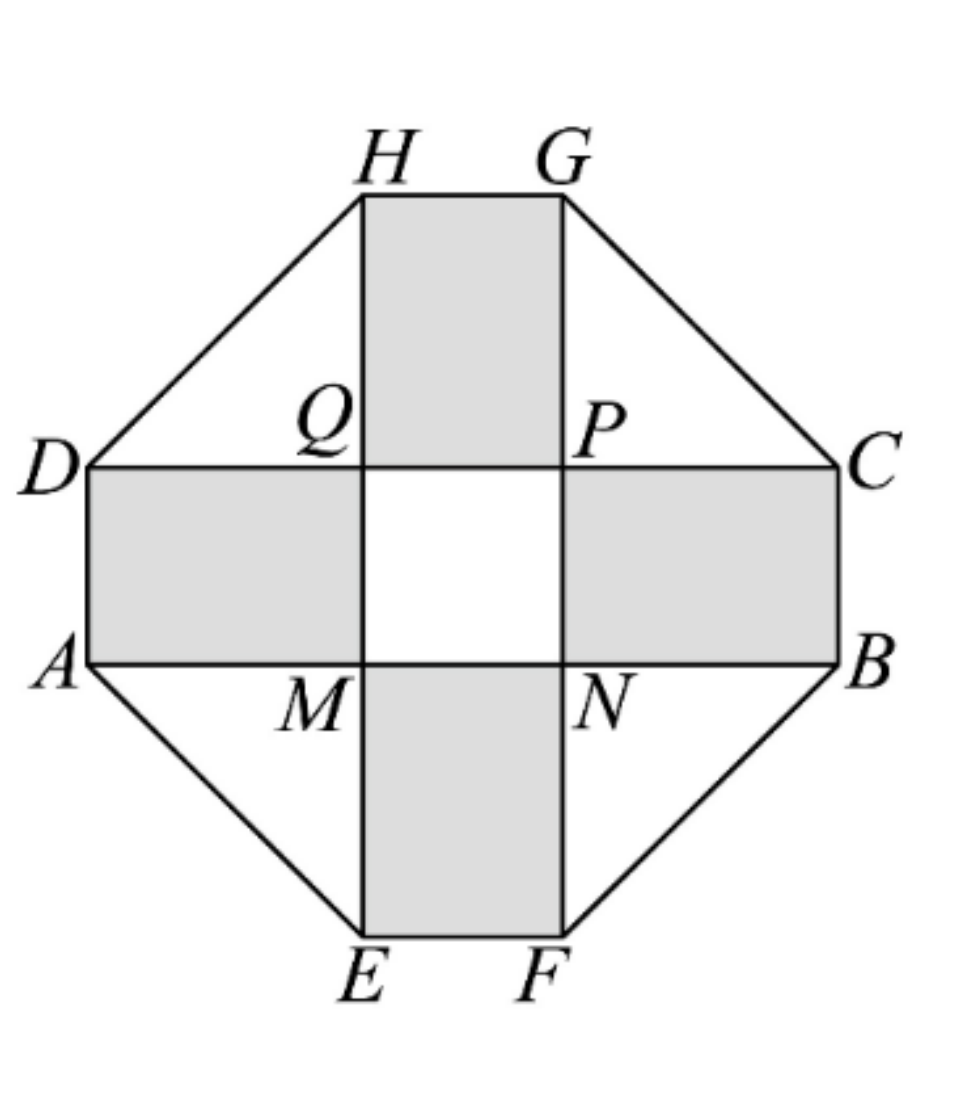
\includegraphics[width=0.34\textwidth]{figures/cross_octagon_h64.png}
\end{center}

\begin{enumerate}[label=(\arabic*)]
\item 设 $DQ$ 长为 $y\mathrm{m}$（$y>0$），用 $x$ 表示 $y$，并求出 $x$ 的取值范围；
\item 如何设计 $AD$ 可使总造价最低，并求出最低造价.
\item 若总造价 $W$ 不超过 69000 元，求 $AD$ 长 $x$ 的取值范围.
\end{enumerate}

\ifanswer
\solbegin
\stepm{(1)}{设 $DQ$ 长为 $y\mathrm{m}$，因为十字形区域面积为 $200\text{m}^2$，}
\step{所以 $4xy+x^2=200$，解得 $y=\dfrac{200-x^2}{4x}=\dfrac{50}{x}-\dfrac x4$；\dots\dots2 分}
\step{因为 $y>0$，所以 $x^2<200$，因为 $x>0$，所以 $0<x<10\sqrt2$.\dots\dots4 分}
\stepm{(2)}{四个矩形地砖面积 $S_{\text{四个矩形}}=4xy=200-x^2$，}
\step{造价 $W_{\text{四个矩形}}=105(200-x^2)$；}
\step{四个三角形草坪面积 $S_{\text{三角形}}=4\times\dfrac12y^2=2\left(\dfrac{50}{x}-\dfrac x4\right)^2=\dfrac{5000}{x^2}+\dfrac{x^2}8-50$，}
\step{造价 $W_{\text{三角形}}=40\left(\dfrac{5000}{x^2}+\dfrac{x^2}8-50\right)$；}
\step{正方形花坛面积 $S_{\text{正方形}}=x^2$，造价 $W_{\text{正方形}}=2100x^2$；}
\step{总造价 $W=W_{\text{四个矩形}}+W_{\text{三角形}}+W_{\text{正方形}}$}
\step{$=105(200-x^2)+40\left(\dfrac{5000}{x^2}+\dfrac{x^2}8-50\right)+2100x^2$，}
\step{化简得 $W=2000x^2+19000+\dfrac{200000}{x^2}$（$0<x<10\sqrt2$）.\dots\dots6 分}
\step{因为 $2000x^2+\dfrac{200000}{x^2}\geqslant40000$，}
\step{当且仅当 $x=\sqrt{10}$（在 $x$ 范围中）时取等号，此时 $W=59000$ 元.}
\step{综上，当 $AD$ 的长为 $\sqrt{10}$ 时，总造价最低，为 59000 元.\dots\dots8 分}
% 原卷 (3) 定义域印作 0<x<2√10，与 (1) 所得 0<x<10√2 不一致，照录（见文件头“原卷笔误”④）
\stepm{(3)}{由（2）得 $W=2000x^2+19000+\dfrac{200000}{x^2}$（$0<x<2\sqrt{10}$）.}
\step{总造价不超过 69000 元，即 $W=2000x^2+19000+\dfrac{200000}{x^2}\leqslant69000$，}
\step{化简得 $x^2+\dfrac{100}{x^2}\leqslant25$，\dots\dots10 分}
\step{即 $(x^2)^2-25x^2+100=(x^2-20)(x^2-5)\leqslant0$，即 $\sqrt5\leqslant x\leqslant2\sqrt5$，}
% 原卷末句“取值范围[√5,2√5]”脱“为”，照录（见文件头“原卷笔误”⑤）
\step{所以 $AD$ 长 $x$ 的取值范围$[\sqrt5,2\sqrt5]$.\dots\dots12 分}
\solend
\fi

\ansspace[10]

\item 设 $a,b,c$ 为实数，集合 $S=\{x\mid(x+a)(x^2+bx+c)=0,x\in\R\}$.

\begin{enumerate}[label=(\arabic*)]
\item 若 $a=1,b=3,c=2$，求集合 $S$；
\item 若 $S=\{-2\}$，求 $a,b,c$ 满足的条件；
\item 设 $T=\{x\mid(ax+1)(cx^2+bx+1)=0,x\in\R\}$，当 $ac\neq0$ 时，如果 $\dfrac12\in S$，$-2\in T$，且
集合 $S,T$ 均恰有两个元素，求三元数对 $(a,b,c)$.
\end{enumerate}

\ifanswer
\solbegin
\stepm{(1)}{若 $a=1,b=3,c=2$，}
\step{则方程 $(x+a)(x^2+bx+c)=0$ 为 $(x+1)(x^2+3x+2)=0$，}
\step{即 $(x+1)^2(x+2)=0$，解得 $x=-1$ 或 $x=-2$，所以 $S=\{-1,-2\}$；}
\stepm{(2)}{由题意得 $-a\in S$，因为 $S=\{-2\}$，所以 $-2$ 是方程 $x+a=0$ 的根，}
\step{即 $-2+a=0$，解得 $a=2$. 由 $S=\{-2\}$，集合 $S$ 有且仅有一个元素，}
\step{即方程 $(x+a)(x^2+bx+c)=0$ 有且仅有一个根，}
\stepm{①}{若 $-2$ 是方程 $x^2+bx+c=0$ 的根，}
\step{则 $\Delta=b^2-4c=0$，且 $-\dfrac b2=-2$，解得 $b=4,c=4$；}
\stepm{②}{若 $-2$ 不是方程 $x^2+bx+c=0$ 的根，则方程 $x^2+bx+c=0$ 无实数根，}
\step{则 $\Delta=b^2-4c<0$，}
\step{综上所述，$\begin{cases}a=2\\ b=4\\ c=4\end{cases}$ 或 $\begin{cases}a=2\\ b^2-4c<0\end{cases}$.}
\stepm{(3)}{$S=\{x\mid(x+a)(x^2+bx+c)=0,x\in\R\}$，}
\step{$T=\{x\mid(ax+1)(cx^2+bx+1)=0,x\in\R\}$，}
\step{由题意得 $a\neq0$ 且 $c\neq0$，则 $-a\in S,-\dfrac1a\in T$，}
\step{且方程 $x^2+bx+c=0$ 与 $cx^2+bx+1=0$ 有相同的判别式 $\Delta=b^2-4c$，}
\step{即两方程根的个数相同. 由集合 $S,T$ 均恰有两个元素，则 $\Delta=b^2-4c\geqslant0$.}
\step{$S=\{x\mid(x+a)(x^2+bx+c)=0,x\in\R\}$，}
\step{因为 $\dfrac12\in S$，所以 $\dfrac12$ 是方程 $x+a=0$ 或 $x^2+bx+c=0$ 的根.}
\step{$T=\{x\mid(ax+1)(cx^2+bx+1)=0,x\in\R\}$，}
\step{由 $-\dfrac1a\in T$，且 $-2\in T$，则 $-2$ 是方程 $ax+1=0$ 或 $cx^2+bx+1=0$ 的根.}
\stepm{①}{当 $a=-\dfrac12$ 时，$\dfrac12$ 是方程 $x+a=0$ 的根，$-a=\dfrac12\in S$，则 $-\dfrac1a=2\in T$，}
\step{又 $-2\in T$，则 $T=\{-2,2\}$，}
\step{由 $T=\left\{x\mid\left(-\dfrac12x+1\right)(cx^2+bx+1)=0,x\in\R\right\}$，}
% 原卷句末为句号，本稿原错作逗号
\step{则 $-2$ 是方程 $cx^2+bx+1=0$ 的根，则 $4c-2b+1=0$.}
\stepm{(i)}{若 $\Delta=b^2-4c=0$，联立 $\begin{cases}4c-2b+1=0\\ b^2-4c=0\end{cases}$ 解得 $b=1,c=\dfrac14$.}
\step{验证：当 $a=-\dfrac12,b=1,c=\dfrac14$ 时，}
\step{$S=\left\{x\mid\left(x-\dfrac12\right)\left(x^2+x+\dfrac14\right)=0,x\in\R\right\}=\left\{-\dfrac12,\dfrac12\right\}$，}
\step{$T=\left\{x\mid\left(-\dfrac12x+1\right)\left(\dfrac14x^2+x+1\right)=0,x\in\R\right\}=\{-2,2\}$，满足题意；}
\stepm{(ii)}{若 $\Delta=b^2-4c>0$，方程 $cx^2+bx+1=0$ 有两个不相等的实数根，}
\step{又 $T=\{-2,2\}$，则方程 $cx^2+bx+1=0$ 的两根必为 $-2$ 和 2.}
\step{由韦达定理得 $\begin{cases}-2+2=-\dfrac bc\\ -2\times2=\dfrac1c\end{cases}$，解得 $b=0,c=-\dfrac14$；}
\step{验证：当 $a=-\dfrac12,b=0,c=-\dfrac14$ 时，}
\step{$S=\left\{x\mid\left(x-\dfrac12\right)\left(x^2-\dfrac14\right)=0,x\in\R\right\}=\left\{-\dfrac12,\dfrac12\right\}$，}
\step{$T=\left\{x\mid\left(-\dfrac12x+1\right)\left(-\dfrac14x^2+1\right)=0,x\in\R\right\}=\{-2,2\}$，满足题意；}
\stepm{②}{当 $a=\dfrac12$ 时，$-\dfrac1a=-2$，即 $-2$ 是方程 $ax+1=0$ 的根，}
\step{则 $-a=-\dfrac12\in S$，又 $\dfrac12\in S$，则 $S=\left\{-\dfrac12,\dfrac12\right\}$，}
\step{$S=\{x\mid(x+a)(x^2+bx+c)=0,x\in\R\}$，}
\step{则 $\dfrac12$ 是方程 $x^2+bx+c=0$ 的根，则 $\dfrac14+\dfrac12b+c=0$，即 $4c+2b+1=0$；}
\stepm{(i)}{若 $\Delta=b^2-4c=0$，联立 $\begin{cases}4c+2b+1=0\\ b^2-4c=0\end{cases}$ 解得 $b=-1,c=\dfrac14$.}
\step{验证：当 $a=\dfrac12,b=-1,c=\dfrac14$ 时，}
\step{$S=\left\{x\mid\left(x+\dfrac12\right)\left(x^2-x+\dfrac14\right)=0,x\in\R\right\}=\left\{-\dfrac12,\dfrac12\right\}$，}
\step{$T=\left\{x\mid\left(\dfrac12x+1\right)\left(\dfrac14x^2-x+1\right)=0,x\in\R\right\}=\{-2,2\}$，满足题意；}
% 原卷作“有两不等的实数根”，本稿原脱“的”
\stepm{(ii)}{若 $\Delta=b^2-4c>0$，方程 $x^2+bx+c=0$ 有两不等的实数根，}
% 原卷句末为句号，本稿原错作逗号
\step{又 $S=\left\{-\dfrac12,\dfrac12\right\}$，则方程 $x^2+bx+c=0$ 的两根必为 $-\dfrac12$ 和 $\dfrac12$.}
\step{由韦达定理得 $\begin{cases}-\dfrac12+\dfrac12=-b\\ -\dfrac12\times\dfrac12=c\end{cases}$，解得 $b=0,c=-\dfrac14$；}
\step{验证：当 $a=\dfrac12,b=0,c=-\dfrac14$ 时，}
\step{$S=\left\{x\mid\left(x+\dfrac12\right)\left(x^2-\dfrac14\right)=0,x\in\R\right\}=\left\{-\dfrac12,\dfrac12\right\}$，}
\step{$T=\left\{x\mid\left(\dfrac12x+1\right)\left(-\dfrac14x^2+1\right)=0,x\in\R\right\}=\{-2,2\}$，满足题意；}
\stepm{③}{当 $a\neq-\dfrac12$ 且 $a\neq\dfrac12$ 时，则 $\dfrac12$ 不是方程 $x+a=0$ 的根，}
\step{$-2$ 也不是方程 $ax+1=0$ 的根.}
% 原卷此句单根而称“两实数根”，语病，照录（见文件头“原卷笔误”⑥）
\step{由 $\dfrac12\in S,-2\in T$，则 $\dfrac12$ 是方程 $x^2+bx+c=0$ 的两实数根，}
\step{且 $-2$ 是方程 $cx^2+bx+1=0$ 的根，则有 $\begin{cases}\dfrac14+\dfrac12b+c=0\\ 4c-2b+1=0\end{cases}$，}
\step{解得 $b=0,c=-\dfrac14$.}
\step{验证：当 $a\neq-\dfrac12$ 且 $a\neq\dfrac12,b=0,c=-\dfrac14$ 时，有 $-a\neq\dfrac12,-a\neq-\dfrac12$.}
\step{$S=\left\{x\mid(x+a)\left(x^2-\dfrac14\right)=0,x\in\R\right\}=\left\{-a,-\dfrac12,\dfrac12\right\}$ 有三个元素，}
\step{故不满足题意；}
\step{综上所述，满足题意的所有三元数对 $(a,b,c)$ 有}
\step{$\left(-\dfrac12,1,\dfrac14\right)$，$\left(-\dfrac12,0,-\dfrac14\right)$，$\left(\dfrac12,-1,\dfrac14\right)$，$\left(\dfrac12,0,-\dfrac14\right)$.}
\solend
\fi

\ansspace*[10]

\end{enumerate}

\end{document}
